\documentclass[letterpaper,10pt,conference]{ieeeconf}
\IEEEoverridecommandlockouts

\usepackage{graphicx,amsmath,amssymb,booktabs,multirow,cite,url,array,xcolor,colortbl,tabularx}
\usepackage[protrusion=false]{microtype}
\usepackage{flushend,flafter}
\usepackage{caption}
\captionsetup[table]{position=bottom,justification=raggedright,singlelinecheck=false,font=small}
\captionsetup[figure]{font=small}
\setlength{\textfloatsep}{8pt plus 2pt minus 2pt}\setlength{\floatsep}{6pt plus 2pt minus 2pt}\setlength{\dbltextfloatsep}{8pt plus 2pt minus 2pt}\setlength{\abovecaptionskip}{3pt}
\usepackage[hidelinks]{hyperref}
\usepackage{tikz}
\usetikzlibrary{arrows.meta,positioning,calc}

\newcommand{\sensor}{\ifdefined\MeshTacAuthorVersion GelSlim~5.0\else sensor~A\fi}
\newcommand{\sensorB}{GelSlim~4.0}
\newcommand{\tableformat}{\small\setlength{\tabcolsep}{3.0pt}\renewcommand{\arraystretch}{1.02}}
\newcommand{\metrichead}[2]{\shortstack[c]{\strut#1\\\strut#2\,$\downarrow$}}
\newcommand{\Kreal}{K}
\newcommand{\todo}[1]{\textcolor{red}{[#1]}}
\renewcommand{\topfraction}{0.95}\renewcommand{\dbltopfraction}{0.95}\renewcommand{\bottomfraction}{0.6}
\renewcommand{\textfraction}{0.03}\renewcommand{\floatpagefraction}{0.75}\renewcommand{\dblfloatpagefraction}{0.75}
\setcounter{topnumber}{4}\setcounter{bottomnumber}{2}\setcounter{totalnumber}{6}\setcounter{dbltopnumber}{3}
% ---- loo ----
\newcommand{\tabloo}{%
Real only (9 objects) & 0.0665 & 0.356 & 0.582 & 30.4 & 64.7 & 4.05 \\
Blender & 0.0657 & 0.346 & 0.592 & 30.3 & 6.8 & \textbf{1.30} \\
Blender (domain rand.) & 0.0635 & 0.342 & 0.601 & 30.4 & 8.9 & 1.56 \\
Blender, bg-norm. & 0.0672 & 0.348 & 0.589 & 30.3 & 5.3 & 1.33 \\
Blender, 1 rotation / object & 0.0645 & 0.354 & 0.585 & 30.4 & 10.3 & 1.61 \\
Blender, 2 rotations / object & 0.0670 & 0.345 & 0.590 & 30.8 & 7.5 & 1.73 \\
GAN-LOO & 0.0631 & 0.331 & 0.618 & 29.9 & 5.7 & 1.45 \\
\quad w/o held-out meshes (control) & 0.0647 & 0.340 & 0.604 & 30.0 & 50.6 & 4.56 \\
Bg-cond.\ GAN-LOO & \textbf{0.0581} & \textbf{0.323} & \textbf{0.633} & \textbf{29.1} & 4.8 & 1.55 \\
GAN-LOO, rotate-then-render & 0.0625 & 0.345 & 0.606 & 29.6 & \textbf{4.4} & 1.37 \\
Multi-sensor GAN-LOO & 0.0695 & 0.358 & 0.579 & 30.9 & 8.6 & 1.62 \\
Blender $\oplus$ GAN-LOO & 0.0661 & 0.349 & 0.601 & 30.7 & 5.6 & 1.40 \\
Refiner (0 labels) & 0.0673 & 0.349 & 0.590 & 30.5 & 7.5 & 1.88 \\
Refiner on domain rand.\ (0 labels, no calib.) & 0.0691 & 0.353 & 0.583 & 30.8 & 7.2 & 1.85 \\
\textit{GAN-full (full real set)} & \textit{0.0467} & \textit{0.277} & \textit{0.676} & \textit{25.8} & \textit{4.6} & \textit{1.41} \\
}

% ---- kshot ----
\newcommand{\tabkshot}{%
0 & Blender only & \textbf{0.0793} & \textbf{0.408} & \textbf{0.572} & \textbf{48.6} & \textbf{8.4} & \textbf{1.82} \\ % pilot150_B_k0_blender (150 ep)
   & \textit{GAN-full (full real set) only} & \textit{0.0459} & \textit{0.274} & \textit{0.705} & \textit{44.6} & \textit{7.0} & \textit{1.62} \\ % pilot150_B_k0_ganfull (150 ep)
\midrule
10 & Real only & 0.0642 & 0.330 & 0.625 & 29.8 & 9.6 & 1.69 \\ % pilot150_B_k10_realonly (150 ep)
  & Blender & 0.0636 & 0.367 & 0.602 & 30.8 & 5.2 & 1.30 \\ % pilot150_B_k10_blender (150 ep)
  & GAN-10 & 0.0624 & 0.354 & 0.597 & 30.6 & 5.9 & 1.44 \\ % pilot150_B_k10_gank (150 ep)
  & Teacher-label self-training & 0.0574 & 0.341 & 0.592 & 28.3 & 6.5 & 1.66 \\ % pilot150_B_k10_semipm_pseudo (150 ep)
  & MeshTac, L1 search & 0.0545 & 0.320 & 0.639 & 27.3 & 4.6 & 1.30 \\ % pilot150_B_k10_rcp (150 ep)
  & MeshTac (ours) & \textbf{0.0521} & 0.293 & 0.660 & \textbf{26.5} & 4.7 & 1.13 \\ % pilot150_B_k10_rf (150 ep)
  & \quad + learned synth. & 0.0559 & \textbf{0.288} & \textbf{0.682} & 27.2 & 4.0 & 1.15 \\ % pilot150_B_k10_al2 (150 ep)
  & \quad synthetic frames for the aligner only & 0.0571 & 0.293 & 0.678 & 27.3 & \textbf{3.2} & \textbf{1.01} \\ % pilot150_B_k10_al0 (150 ep)
   & \textit{GAN-full (full real set)} & \textit{0.0484} & \textit{0.281} & \textit{0.693} & \textit{28.5} & \textit{6.1} & \textit{1.50} \\ % pilot_B_k10_ganfull (50 ep)
\midrule
25 & Real only & 0.0558 & 0.312 & 0.664 & 28.2 & 5.6 & 1.21 \\ % pilot150_B_k25_realonly (150 ep)
  & Blender & 0.0549 & 0.329 & 0.656 & 27.5 & 4.7 & 1.10 \\ % pilot150_B_k25_blender (150 ep)
  & GAN-25 & 0.0544 & 0.321 & 0.626 & 28.3 & 5.1 & 1.20 \\ % pilot150_B_k25_gank (150 ep)
  & Blender $\oplus$ GAN-25 & 0.0554 & 0.324 & 0.667 & 27.4 & 4.8 & 1.14 \\ % pilot150_B_k25_mix (150 ep)
  & Refiner-25 (0 labels) & 0.0551 & 0.297 & 0.672 & 27.1 & 5.5 & 1.30 \\ % pilot150_B_k25_ref (150 ep)
  & Refiner-U (0 labels, all unlabeled) & 0.0566 & 0.309 & 0.666 & 27.8 & 5.6 & 1.31 \\ % pilot150_B_k25_refufull (150 ep)
  & Self-trained GAN-25 (renderer only) & 0.0538 & 0.326 & 0.641 & 28.0 & 4.8 & 1.14 \\ % pilot150_B_k25_pseudo (150 ep)
  & Teacher-label self-training, model only & 0.0517 & 0.300 & 0.611 & 26.5 & 8.2 & 1.55 \\ % pilot150_B_k25_semipm (150 ep)
  & \quad center window only (no stitching) & 0.0518 & 0.328 & 0.643 & 26.7 & 8.4 & 1.55 \\ % pilot150_B_k25_semipm_c1 (150 ep)
  & Teacher-label self-training & 0.0508 & 0.307 & 0.628 & 26.5 & 6.1 & 1.54 \\ % pilot150_B_k25_semipm_pseudo (150 ep)
  & \quad round 2 & 0.0500 & 0.310 & 0.642 & 26.0 & 6.2 & 1.54 \\ % pilot150_B_k25_semipm_pseudo_r2 (150 ep)
  & MeshTac, L1 search & 0.0482 & 0.291 & 0.655 & 25.5 & 4.5 & 1.16 \\ % pilot150_B_k25_rcp (150 ep)
  & MeshTac (ours) & \textbf{0.0433} & \textbf{0.245} & 0.726 & \textbf{23.3} & 2.8 & 0.91 \\ % pilot150_B_k25_rf (150 ep)
  & \quad + learned synth. & 0.0450 & 0.249 & \textbf{0.727} & 24.0 & 3.7 & 1.00 \\ % pilot150_B_k25_al2 (150 ep)
  & \quad synthetic frames for the aligner only & 0.0456 & 0.259 & 0.715 & 24.7 & \textbf{2.7} & \textbf{0.85} \\ % pilot150_B_k25_al0 (150 ep)
   & \textit{GAN-full (full real set)} & \textit{0.0417} & \textit{0.262} & \textit{0.724} & \textit{25.5} & \textit{4.9} & \textit{1.14} \\ % pilot150_B_k25_ganfull (150 ep)
\midrule
50 & Real only & 0.0482 & 0.283 & 0.690 & 25.5 & 4.3 & 0.91 \\ % pilot150_B_k50_realonly (150 ep)
  & Blender & 0.0478 & 0.270 & 0.701 & 25.2 & 4.5 & 1.02 \\ % pilot150_B_k50_blender (150 ep)
  & GAN-50 & 0.0434 & 0.260 & 0.716 & 24.3 & 4.7 & 1.10 \\ % pilot150_B_k50_gank (150 ep)
  & Teacher-label self-training & 0.0381 & 0.255 & 0.706 & 22.7 & 5.5 & 1.36 \\ % pilot150_B_k50_semipm_pseudo (150 ep)
  & MeshTac, L1 search & 0.0384 & 0.247 & 0.714 & 22.7 & 4.1 & 1.03 \\ % pilot150_B_k50_rcp (150 ep)
  & MeshTac (ours) & \textbf{0.0291} & \textbf{0.197} & 0.761 & \textbf{19.8} & \textbf{2.7} & \textbf{0.74} \\ % pilot150_B_k50_rf (150 ep)
  & \quad + learned synth. & 0.0307 & 0.206 & \textbf{0.769} & 20.4 & 3.7 & 0.95 \\ % pilot150_B_k50_al2 (150 ep)
  & \quad synthetic frames for the aligner only & 0.0332 & 0.215 & 0.764 & 21.1 & 3.0 & 0.77 \\ % pilot150_B_k50_al0 (150 ep)
   & \textit{GAN-full (full real set)} & \textit{0.0363} & \textit{0.239} & \textit{0.747} & \textit{22.7} & \textit{4.7} & \textit{1.07} \\ % pilot150_B_k50_ganfull (150 ep)
\midrule
100 & Real only & 0.0369 & 0.235 & 0.744 & 22.1 & 3.2 & 0.72 \\ % pilot150_B_k100_realonly (150 ep)
  & Blender & 0.0350 & 0.232 & 0.727 & 22.0 & 4.0 & 1.04 \\ % pilot150_B_k100_blender (150 ep)
  & GAN-100 & 0.0311 & 0.210 & 0.773 & 20.8 & 4.5 & 1.03 \\ % pilot150_B_k100_gank (150 ep)
  & Blender $\oplus$ GAN-100 & 0.0329 & 0.213 & 0.760 & 20.5 & 4.2 & 0.99 \\ % pilot150_B_k100_mix (150 ep)
  & Refiner-100 (0 labels) & 0.0340 & 0.224 & 0.761 & 21.1 & 4.9 & 1.20 \\ % pilot150_B_k100_ref (150 ep)
  & Refiner-U (0 labels, all unlabeled) & 0.0329 & 0.228 & 0.747 & 21.1 & 4.9 & 1.16 \\ % pilot150_B_k100_refufull (150 ep)
  & Self-trained GAN-100 (renderer only) & 0.0308 & 0.207 & 0.774 & 20.6 & 4.4 & 1.01 \\ % pilot150_B_k100_pseudo (150 ep)
  & Teacher-label self-training, model only & 0.0290 & 0.221 & 0.744 & 19.8 & 4.5 & 1.09 \\ % pilot150_B_k100_semipm (150 ep)
  & Teacher-label self-training & 0.0285 & 0.211 & 0.750 & 19.7 & 4.9 & 1.16 \\ % pilot150_B_k100_semipm_pseudo (150 ep)
  & \quad round 2 & 0.0295 & 0.217 & 0.736 & 20.2 & 4.9 & 1.15 \\ % pilot150_B_k100_semipm_pseudo_r2 (150 ep)
  & MeshTac, L1 search & 0.0276 & 0.203 & 0.771 & 19.4 & 4.1 & 0.97 \\ % pilot150_B_k100_rcp (150 ep)
  & MeshTac (ours) & \textbf{0.0227} & \textbf{0.166} & \textbf{0.818} & \textbf{16.9} & \textbf{2.5} & \textbf{0.70} \\ % pilot150_B_k100_rf (150 ep)
  & \quad + learned synth. & 0.0232 & 0.168 & 0.803 & 17.1 & 3.7 & 0.91 \\ % pilot150_B_k100_al2 (150 ep)
  & \quad synthetic frames for the aligner only & 0.0237 & 0.168 & 0.809 & 17.1 & 2.7 & 0.71 \\ % pilot150_B_k100_al0 (150 ep)
   & \textit{GAN-full (full real set)} & \textit{0.0274} & \textit{0.205} & \textit{0.777} & \textit{19.9} & \textit{4.4} & \textit{1.01} \\ % pilot150_B_k100_ganfull (150 ep)
}

% ---- seeds ----
\newcommand{\tabseeds}{%
25 & Real only & 0.0551 $\pm$ 0.0010 & 0.314 $\pm$ 0.010 & 0.665 $\pm$ 0.004 & 5.5 $\pm$ 0.0 \\
25 & GAN-25 & 0.0536 $\pm$ 0.0013 & 0.314 $\pm$ 0.008 & 0.655 $\pm$ 0.032 & 6.0 $\pm$ 0.1 \\
25 & Teacher-label self-training & 0.0507 $\pm$ 0.0001 & 0.310 $\pm$ 0.004 & 0.624 $\pm$ 0.002 & 7.2 $\pm$ 0.1 \\
25 & MeshTac, L1 search & 0.0482 $\pm$ 0.0004 & 0.289 $\pm$ 0.004 & 0.648 $\pm$ 0.010 & 5.5 $\pm$ 0.1 \\
25 & MeshTac & 0.0433 $\pm$ 0.0004 & 0.247 $\pm$ 0.000 & 0.722 $\pm$ 0.000 & 4.0 $\pm$ 0.0 \\
25 & \quad + learned synth. & 0.0447 $\pm$ 0.0009 & 0.246 $\pm$ 0.002 & 0.729 $\pm$ 0.002 & 4.9 $\pm$ 0.1 \\
100 & Real only & 0.0366 $\pm$ 0.0008 & 0.234 $\pm$ 0.006 & 0.750 $\pm$ 0.004 & 3.9 $\pm$ 0.0 \\
100 & GAN-100 & 0.0299 $\pm$ 0.0004 & 0.201 $\pm$ 0.002 & 0.779 $\pm$ 0.001 & 5.5 $\pm$ 0.0 \\
100 & Teacher-label self-training & 0.0280 $\pm$ 0.0001 & 0.209 $\pm$ 0.002 & 0.743 $\pm$ 0.007 & 6.1 $\pm$ 0.0 \\
100 & MeshTac, L1 search & 0.0275 $\pm$ 0.0002 & 0.201 $\pm$ 0.003 & 0.767 $\pm$ 0.005 & 5.0 $\pm$ 0.1 \\
100 & MeshTac & 0.0222 $\pm$ 0.0004 & 0.163 $\pm$ 0.002 & 0.821 $\pm$ 0.002 & 3.8 $\pm$ 0.0 \\
100 & \quad + learned synth. & 0.0229 $\pm$ 0.0003 & 0.164 $\pm$ 0.000 & 0.818 $\pm$ 0.000 & 4.8 $\pm$ 0.0 \\
}

% ---- rcabl ----
\newcommand{\tabrcabl}{%
teacher & -- & 0.56 & 0.32 & -- & 0.0507 & 0.310 & 0.624 & 7.2 \\
teacher & teacher & 0.56 & 0.32 & 4.9 & 0.0508 & 0.310 & 0.622 & 5.9 \\
\midrule
mesh & teacher pose & 0.47 & 0.40 & 6.0 & 0.0641 & 0.384 & 0.497 & 5.7 \\
mesh$^{1/2}$ & L1$^{1/2}$ & 0.63 & 0.30 & 1.4 & 0.0485 & 0.286 & 0.639 & 6.3 \\
mesh & L1 & 0.64 & 0.30 & 2.5 & 0.0489 & 0.292 & 0.657 & 5.4 \\
mesh$^{1/2}$ & L1 & 0.63 & 0.30 & 2.5 & 0.0482 & 0.289 & 0.648 & 5.5 \\
\midrule
mesh & aligner$^{\ddagger}$ & 0.71 & 0.24 & 1.1 & 0.0447 & 0.248 & 0.730 & 5.0 \\
mesh & aligner$^{\dagger}$ & 0.71 & 0.24 & 1.1 & 0.0447 & 0.246 & 0.729 & 4.9 \\
mesh & aligner, no renderer & 0.72 & 0.23 & 1.1 & 0.0433 & 0.247 & 0.722 & 4.0 \\
}

% ---- cross ----
\newcommand{\tabcross}{%
Real only (9 objects, session 1) & 0.315 & 0.675 & 25.4 & 12.6 & 7.7 \\
Blender & 0.294 & 0.701 & 24.9 & 9.5 & 5.1 \\
Blender (domain rand.) & 0.294 & 0.691 & 25.5 & 10.3 & 5.5 \\
Blender, bg-norm. & 0.291 & 0.698 & 24.9 & 9.1 & \textbf{4.5} \\
GAN-LOO & 0.272 & 0.723 & 24.1 & 10.8 & 5.2 \\
Bg-cond.\ GAN-LOO & 0.270 & 0.727 & 24.2 & 10.4 & 4.7 \\
Blender $\oplus$ GAN-LOO & 0.275 & 0.724 & 24.0 & 10.2 & 5.0 \\
Refiner (0 labels) & 0.290 & 0.714 & 24.6 & 11.6 & 5.1 \\
\textit{GAN-full (full real set)} & \textit{0.259} & \textit{0.748} & \textit{22.9} & \textit{9.9} & \textit{4.8} \\
\midrule
Blender only ($\Kreal=0$) & 0.425 & 0.561 & 50.7 & 11.7 & 6.0 \\
$\Kreal=25$ real only & 0.368 & 0.598 & 30.7 & 16.2 & 5.7 \\
$\Kreal=25$ + Blender & 0.382 & 0.615 & 30.1 & 9.7 & 5.0 \\
$\Kreal=25$ + GAN-25 & 0.342 & 0.589 & 28.7 & 10.2 & 5.0 \\
$\Kreal=25$ + refiner-25 (0 labels) & 0.338 & 0.635 & 29.5 & 12.1 & 5.4 \\
$\Kreal=25$ + self-trained GAN-25 & 0.363 & 0.606 & 29.1 & 11.6 & 5.2 \\
$\Kreal=25$ + teacher-label self-training & 0.335 & 0.598 & 27.5 & 12.0 & 4.7 \\
$\Kreal=25$ + MeshTac, L1 search & 0.322 & 0.621 & 27.4 & 10.1 & 4.6 \\
$\Kreal=25$ + MeshTac & 0.306 & 0.654 & 27.3 & 10.9 & 6.0 \\
$\Kreal=25$ + MeshTac + learned synth. & 0.310 & 0.660 & 27.2 & \textbf{9.0} & 4.6 \\
$\Kreal=100$ real only & 0.351 & 0.657 & 27.5 & 12.9 & 7.3 \\
$\Kreal=100$ + Blender & 0.299 & 0.647 & 25.3 & 9.8 & 4.7 \\
$\Kreal=100$ + GAN-100 & 0.295 & 0.713 & 25.6 & 11.1 & 5.1 \\
$\Kreal=100$ + refiner-100 (0 labels) & 0.330 & 0.688 & 26.2 & 11.6 & 4.8 \\
$\Kreal=100$ + self-trained GAN-100 & 0.310 & 0.715 & 26.1 & 10.7 & 5.0 \\
$\Kreal=100$ + teacher-label self-training & 0.300 & 0.707 & 24.2 & 10.9 & 4.9 \\
$\Kreal=100$ + MeshTac, L1 search & 0.293 & 0.718 & 23.5 & 10.5 & 4.6 \\
$\Kreal=100$ + MeshTac & 0.288 & 0.707 & 24.6 & 10.1 & 6.0 \\
$\Kreal=100$ + MeshTac + learned synth. & \textbf{0.252} & \textbf{0.743} & \textbf{22.8} & 10.2 & 5.0 \\
}

% ---- kshotmain ----
\newcommand{\tabkshotmain}{%
10 & Real only & 0.0642 & 0.330 & 0.625 & 29.8 & 9.6 & 1.69 \\
  & PBR & 0.0636 & 0.367 & 0.602 & 30.8 & 5.2 & 1.30 \\
  & Learned renderer & 0.0624 & 0.354 & 0.597 & 30.6 & 5.9 & 1.44 \\
  & Self-training & 0.0574 & 0.341 & 0.592 & 28.3 & 6.5 & 1.66 \\
  & MeshTac (ours) & 0.0559 & \textbf{0.288} & \textbf{0.682} & 27.2 & \textbf{4.0} & 1.15 \\
  & \quad no renderer & \textbf{0.0521} & 0.293 & 0.660 & \textbf{26.5} & 4.7 & \textbf{1.13} \\
   & \textit{Learned renderer (full)} & \textit{0.0484} & \textit{0.281} & \textit{0.693} & \textit{28.5} & \textit{6.1} & \textit{1.50} \\
\midrule
25 & Real only & 0.0558 & 0.312 & 0.664 & 28.2 & 5.6 & 1.21 \\
  & PBR & 0.0549 & 0.329 & 0.656 & 27.5 & 4.7 & 1.10 \\
  & Learned renderer & 0.0544 & 0.321 & 0.626 & 28.3 & 5.1 & 1.20 \\
  & Self-training & 0.0508 & 0.307 & 0.628 & 26.5 & 6.1 & 1.54 \\
  & MeshTac (ours) & 0.0450 & 0.249 & \textbf{0.727} & 24.0 & 3.7 & 1.00 \\
  & \quad no renderer & \textbf{0.0433} & \textbf{0.245} & 0.726 & \textbf{23.3} & \textbf{2.8} & \textbf{0.91} \\
   & \textit{Learned renderer (full)} & \textit{0.0417} & \textit{0.262} & \textit{0.724} & \textit{25.5} & \textit{4.9} & \textit{1.14} \\
\midrule
50 & Real only & 0.0482 & 0.283 & 0.690 & 25.5 & 4.3 & 0.91 \\
  & PBR & 0.0478 & 0.270 & 0.701 & 25.2 & 4.5 & 1.02 \\
  & Learned renderer & 0.0434 & 0.260 & 0.716 & 24.3 & 4.7 & 1.10 \\
  & Self-training & 0.0381 & 0.255 & 0.706 & 22.7 & 5.5 & 1.36 \\
  & MeshTac (ours) & 0.0307 & 0.206 & \textbf{0.769} & 20.4 & 3.7 & 0.95 \\
  & \quad no renderer & \textbf{0.0291} & \textbf{0.197} & 0.761 & \textbf{19.8} & \textbf{2.7} & \textbf{0.74} \\
   & \textit{Learned renderer (full)} & \textit{0.0363} & \textit{0.239} & \textit{0.747} & \textit{22.7} & \textit{4.7} & \textit{1.07} \\
\midrule
100 & Real only & 0.0369 & 0.235 & 0.744 & 22.1 & 3.2 & 0.72 \\
  & PBR & 0.0350 & 0.232 & 0.727 & 22.0 & 4.0 & 1.04 \\
  & Learned renderer & 0.0311 & 0.210 & 0.773 & 20.8 & 4.5 & 1.03 \\
  & Self-training & 0.0285 & 0.211 & 0.750 & 19.7 & 4.9 & 1.16 \\
  & MeshTac (ours) & 0.0232 & 0.168 & 0.803 & 17.1 & 3.7 & 0.91 \\
  & \quad no renderer & \textbf{0.0227} & \textbf{0.166} & \textbf{0.818} & \textbf{16.9} & \textbf{2.5} & \textbf{0.70} \\
   & \textit{Learned renderer (full)} & \textit{0.0274} & \textit{0.205} & \textit{0.777} & \textit{19.9} & \textit{4.4} & \textit{1.01} \\
}

% ---- crossmain ----
\newcommand{\tabcrossmain}{%
$\dagger$ & Real only & 0.315 & 0.675 & 25.4 & 12.6 \\
  & PBR & 0.294 & 0.701 & 24.9 & 9.5 \\
  & Learned renderer & 0.270 & 0.727 & 24.2 & 10.4 \\
   & \textit{Learned renderer (full)} & \textit{0.259} & \textit{0.748} & \textit{22.9} & \textit{9.9} \\
\midrule
25 & Real only & 0.368 & 0.598 & 30.7 & 16.2 \\
  & Learned renderer & 0.342 & 0.589 & 28.7 & 10.2 \\
  & Self-training & 0.335 & 0.598 & 27.5 & 12.0 \\
  & MeshTac (ours) & 0.310 & 0.660 & 27.2 & \textbf{9.0} \\
  & \quad no renderer & 0.306 & 0.654 & 27.3 & 10.9 \\
\midrule
100 & Real only & 0.351 & 0.657 & 27.5 & 12.9 \\
  & Learned renderer & 0.295 & 0.713 & 25.6 & 11.1 \\
  & Self-training & 0.300 & 0.707 & 24.2 & 10.9 \\
  & MeshTac (ours) & \textbf{0.252} & \textbf{0.743} & \textbf{22.8} & 10.2 \\
  & \quad no renderer & 0.288 & 0.707 & 24.6 & 10.1 \\
}

% ---- loomain ----
\newcommand{\tabloomain}{%
Real only (9 objects) & 0.0665 & 0.356 & 0.582 & 64.7 \\
PBR & 0.0657 & 0.346 & 0.592 & 6.8 \\
Learned renderer & 0.0631 & 0.331 & 0.618 & 5.7 \\
\quad w/o held-out meshes & 0.0647 & 0.340 & 0.604 & 50.6 \\
\quad + background & \textbf{0.0581} & \textbf{0.323} & \textbf{0.633} & \textbf{4.8} \\
\textit{Learned renderer (full)} & \textit{0.0467} & \textit{0.277} & \textit{0.676} & \textit{4.6} \\
}

% ---- rcablmain ----
\newcommand{\tabrcablmain}{%
\multicolumn{8}{@{}l}{\emph{Teacher predictions as labels (self-training)}} \\
\quad depth & 0.56 & 0.32 & -- & 0.0507 & 0.310 & 0.624 & 7.2 \\
\quad depth + pose & 0.56 & 0.32 & 4.9 & 0.0508 & 0.310 & 0.622 & 5.9 \\
\multicolumn{8}{@{}l}{\emph{Mesh projected at a fitted pose}} \\
\quad pose by the teacher (no alignment) & 0.47 & 0.40 & 6.0 & 0.0641 & 0.384 & 0.497 & 5.7 \\
\quad pose by L1 render-and-compare$^{1/2}$ & 0.63 & 0.30 & 2.5 & 0.0482 & 0.289 & 0.648 & 5.5 \\
\quad pose by learned aligner (MeshTac) & 0.72 & 0.23 & 1.1 & 0.0433 & 0.247 & 0.722 & 4.0 \\
\quad\quad + learned synth.$^{\ddagger}$ & 0.71 & 0.24 & 1.1 & 0.0447 & 0.246 & 0.729 & 4.9 \\
}

% ---- rcabl2 ----
\newcommand{\tabrcablii}{%
Teacher & -- & 0.56 & 0.32 & -- & -- & 0.63 & 0.30 & 11.1 & 1.7 \\
Teacher & Teacher & 0.56 & 0.32 & 4.9 & 1.0 & 0.63 & 0.30 & 6.2 & 1.2 \\
Mesh & Teacher & 0.47 & 0.40 & 6.0 & 1.1 & 0.51 & 0.36 & 6.0 & 1.2 \\
Mesh & L1 search & 0.63 & 0.30 & 2.5 & 0.80 & 0.66 & 0.29 & 5.4 & 1.2 \\
\rowcolor{gray!12} Mesh & Aligner (ours) & \textbf{0.72} & \textbf{0.23} & \textbf{1.1} & \textbf{0.67} & \textbf{0.74} & \textbf{0.23} & \textbf{4.2} & \textbf{1.0} \\
}

% ---- poseref ----
\newcommand{\tabposeref}{%
\multicolumn{9}{@{}l}{\emph{Rotation error (deg)}} \\
10 & 9.9 & 2.5 & 4.3 & 2.2 & 20.4 & 12.6 & 15.0 & 9.3 \\
25 & 5.7 & 1.1 & 3.2 & 0.8 & 16.2 & 6.9 & 10.9 & 5.3 \\
50 & 4.2 & 0.6 & 3.1 & 0.9 & 13.0 & 6.6 & 11.5 & 7.2 \\
100 & 3.3 & 0.4 & 2.9 & 0.4 & 12.6 & 5.5 & 10.1 & 4.2 \\
\midrule
\multicolumn{9}{@{}l}{\emph{Translation error (mm)}} \\
10 & 1.59 & 0.84 & 0.98 & 0.78 & 2.22 & 1.70 & 2.01 & 1.59 \\
25 & 1.09 & 0.65 & 0.88 & 0.63 & 2.00 & 1.33 & 1.68 & 1.24 \\
50 & 0.73 & 0.40 & 0.66 & 0.44 & 1.95 & 1.41 & 1.69 & 1.30 \\
100 & 0.63 & 0.28 & 0.62 & 0.28 & 1.86 & 1.31 & 1.73 & 1.21 \\
}

% ---- sensorb ----
\newcommand{\tabsensorb}{%
0 & Sensor-A model, real only & 0.1486 & 0.513 & 0.280 & 25.7 & 11.6 \\
  & Sensor-A model, Blender only & 0.1175 & 0.413 & 0.370 & 34.3 & 11.6 \\
\midrule
10 & Real only & 0.0248 & 0.165 & 0.803 & 20.5 & 11.1 \\
  & Blender (sensor-A calib.) & 0.0266 & 0.168 & 0.803 & 20.0 & 11.5 \\
  & GAN-10 (sensor B) & 0.0237 & 0.155 & 0.809 & 19.0 & 11.3 \\
\midrule
25 & Real only & 0.0152 & 0.139 & 0.824 & 17.2 & 10.9 \\
  & Blender (sensor-A calib.) & 0.0147 & 0.125 & 0.846 & 16.5 & 11.2 \\
  & Blender (domain rand.) & 0.0146 & 0.126 & 0.830 & 16.3 & 10.9 \\
  & GAN-25 (sensor B) & 0.0107 & 0.100 & 0.846 & 14.6 & 10.4 \\
  & Teacher-label self-training, model only & 0.0098 & 0.100 & 0.841 & 14.8 & 11.6 \\
  & Teacher-label self-training & 0.0102 & 0.098 & 0.840 & 14.6 & 11.8 \\
\midrule
50 & Real only & 0.0063 & 0.081 & 0.860 & 13.2 & 9.9 \\
  & Blender (sensor-A calib.) & 0.0058 & 0.077 & 0.858 & 12.8 & 9.7 \\
  & GAN-50 (sensor B) & 0.0045 & 0.068 & 0.866 & 12.1 & 10.1 \\
\midrule
100 & Real only & \textbf{0.0032} & 0.058 & 0.861 & \textbf{11.0} & \textbf{7.5} \\
  & Blender (sensor-A calib.) & 0.0033 & \textbf{0.057} & 0.868 & 11.0 & 9.3 \\
  & Blender (domain rand.) & 0.0036 & 0.062 & 0.866 & 11.4 & 10.6 \\
  & GAN-100 (sensor B) & 0.0034 & 0.060 & \textbf{0.870} & 11.2 & 10.1 \\
}

% ---- variants ----
\newcommand{\tabvariants}{%
Real only & -- & 0.312 & -- & 0.356 & 64.7 \\
GAN-$\Kreal$ / GAN-LOO & 0.108 & 0.321 & 0.068 & 0.331 & 5.7 \\
\quad Blender-pretrained & 0.111 & 0.335 & 0.084 & 0.356 & 8.5 \\
\quad difference image & 0.108 & 0.339 & 0.066 & 0.346 & 6.3 \\
\quad background-conditioned & \textbf{0.101} & 0.330 & \textbf{0.062} & \textbf{0.323} & \textbf{4.8} \\
\quad physics-conditioned & 0.114 & -- & -- & -- & -- \\
\quad physics residual & 0.119 & -- & -- & -- & -- \\
\quad physics + background & 0.104 & -- & -- & -- & -- \\
\quad self-trained (+ pseudo pairs) & 0.102 & 0.326 & -- & -- & -- \\
Refiner, unpaired (0 labels) & 0.159 & 0.297 & 0.159 & 0.349 & 7.5 \\
\quad + self-regularization & -- & -- & 0.156 & 0.360 & 7.4 \\
\quad on domain-rand.\ render & -- & -- & 0.159 & 0.353 & 7.2 \\
Blender (calibrated) & -- & 0.329 & 0.179 & 0.346 & 6.8 \\
Blender (domain rand.) & -- & 0.320 & -- & 0.342 & 8.9 \\
Blender, bg-norm. & -- & 0.338 & -- & 0.348 & 5.3 \\
Real only, mask head + grad.\ loss & -- & 0.309 & -- & -- & -- \\
GAN-$\Kreal$, mask head + grad.\ loss & -- & 0.302 & -- & -- & -- \\
Blender pretrain $\to$ real fine-tune & -- & \textbf{0.294} & -- & -- & -- \\
\quad + L2-SP & -- & 0.307 & -- & -- & -- \\
}

% ---- sbmapl ----
\newcommand{\tabsbmapl}{%
10 & Real only & 0.0314 & 0.180 & 0.780 & 22.5 & 11.4 \\
  & Learned renderer & 0.0290 & 0.173 & 0.801 & 21.7 & 12.0 \\
  & Self-training & 0.0301 & 0.202 & 0.773 & 22.5 & 13.2 \\
  & MeshTac (ours) & \textbf{0.0170} & \textbf{0.121} & \textbf{0.856} & \textbf{19.7} & \textbf{8.7} \\
\midrule
25 & Real only & 0.0182 & 0.127 & 0.847 & 19.6 & 8.6 \\
  & Learned renderer & 0.0148 & 0.111 & 0.877 & 18.3 & 10.6 \\
  & Self-training & 0.0175 & 0.135 & 0.846 & 19.7 & 13.0 \\
  & MeshTac (ours) & 0.0076 & 0.081 & \textbf{0.911} & 16.3 & \textbf{8.3} \\
  & \quad + learned synth. & \textbf{0.0075} & \textbf{0.078} & 0.904 & \textbf{16.2} & 9.5 \\
\midrule
50 & Real only & 0.0088 & 0.083 & 0.899 & 16.9 & \textbf{7.3} \\
  & Learned renderer & 0.0070 & 0.075 & 0.910 & 16.0 & 9.7 \\
  & Self-training & 0.0081 & 0.084 & 0.901 & 16.4 & 12.4 \\
  & MeshTac (ours) & \textbf{0.0041} & \textbf{0.061} & \textbf{0.933} & \textbf{14.8} & 8.2 \\
\midrule
100 & Real only & 0.0051 & 0.066 & 0.932 & 15.1 & \textbf{8.0} \\
  & Learned renderer & 0.0052 & 0.063 & 0.928 & 15.0 & 9.8 \\
  & Self-training & 0.0047 & 0.070 & 0.933 & 14.9 & 11.5 \\
  & MeshTac (ours) & \textbf{0.0034} & \textbf{0.056} & \textbf{0.944} & \textbf{14.4} & 8.1 \\
}

% ---- sbseeds ----
\newcommand{\tabsbseeds}{%
10 & Real only & 0.0317\,\scalebox{0.8}{$\pm$0.0003} & 0.181\,\scalebox{0.8}{$\pm$0.006} & 0.780\,\scalebox{0.8}{$\pm$0.001} & 13.5\,\scalebox{0.8}{$\pm$0.4} \\
10 & MeshTac & 0.0169\,\scalebox{0.8}{$\pm$0.0001} & 0.121\,\scalebox{0.8}{$\pm$0.0003} & 0.855\,\scalebox{0.8}{$\pm$0.0002} & 10.1\,\scalebox{0.8}{$\pm$0.5} \\
25 & Real only & 0.0179\,\scalebox{0.8}{$\pm$0.0004} & 0.127\,\scalebox{0.8}{$\pm$0.001} & 0.849\,\scalebox{0.8}{$\pm$0.002} & 12.3\,\scalebox{0.8}{$\pm$0.8} \\
25 & MeshTac & 0.0076\,\scalebox{0.8}{$\pm$0.0001} & 0.082\,\scalebox{0.8}{$\pm$0.002} & 0.912\,\scalebox{0.8}{$\pm$0.001} & 9.0\,\scalebox{0.8}{$\pm$0.1} \\
50 & Real only & 0.0089\,\scalebox{0.8}{$\pm$0.0001} & 0.084\,\scalebox{0.8}{$\pm$0.002} & 0.900\,\scalebox{0.8}{$\pm$0.001} & 9.2\,\scalebox{0.8}{$\pm$0.5} \\
50 & MeshTac & 0.0041\,\scalebox{0.8}{$\pm$0.0001} & 0.063\,\scalebox{0.8}{$\pm$0.002} & 0.933\,\scalebox{0.8}{$\pm$0.001} & 9.8\,\scalebox{0.8}{$\pm$0.05} \\
100 & Real only & 0.0050\,\scalebox{0.8}{$\pm$0.0001} & 0.067\,\scalebox{0.8}{$\pm$0.002} & 0.933\,\scalebox{0.8}{$\pm$0.0001} & 9.3\,\scalebox{0.8}{$\pm$0.7} \\
100 & MeshTac & 0.0033\,\scalebox{0.8}{$\pm$0.00002} & 0.054\,\scalebox{0.8}{$\pm$0.002} & 0.944\,\scalebox{0.8}{$\pm$0.0003} & 9.4\,\scalebox{0.8}{$\pm$0.4} \\
}

% ---- selection ----
\newcommand{\tabselection}{%
Real only, selection 0 & 0.0558 & 0.303 & 0.666 \\
Real only, selection 1 & 0.0578 & 0.314 & 0.655 \\
Real only, selection 2 & 0.0585 & 0.324 & 0.650 \\
MeshTac, selection 0 & 0.0435 & 0.247 & 0.722 \\
MeshTac, selection 1 & 0.0426 & 0.252 & 0.724 \\
MeshTac, selection 2 & 0.0425 & 0.244 & 0.718 \\
}

% ---- kshotshort ----
\newcommand{\tabkshotshort}{%
10 & Real only & 0.0573 & 0.313 & 0.645 & 28.8 & 9.9 & 1.59 \\
  & Learned renderer ($K$) & 0.0559 & 0.331 & 0.608 & 30.0 & 5.9 & 1.28 \\
  & Self-training & 0.0525 & 0.332 & 0.601 & 27.8 & 13.2 & 1.90 \\
  & MeshTac (ours) & \textbf{0.0470} & \textbf{0.265} & \textbf{0.696} & \textbf{25.2} & 4.3 & \textbf{0.98} \\
  & \quad + learned synth. & 0.0484 & 0.279 & 0.684 & 27.5 & \textbf{4.2} & 1.04 \\
   & \textit{Learned renderer (full)} & \textit{0.0444} & \textit{0.272} & \textit{0.701} & \textit{26.9} & \textit{6.5} & \textit{1.32} \\
\midrule
25 & Real only & 0.0489 & 0.291 & 0.676 & 27.4 & 5.7 & 1.09 \\
  & Learned renderer ($K$) & 0.0481 & 0.298 & 0.617 & 28.4 & 5.3 & 1.04 \\
  & Self-training & 0.0462 & 0.301 & 0.641 & 25.9 & 8.6 & 1.51 \\
  & MeshTac (ours) & \textbf{0.0383} & \textbf{0.233} & \textbf{0.737} & \textbf{23.1} & \textbf{3.2} & \textbf{0.88} \\
  & \quad + learned synth. & 0.0394 & 0.240 & 0.726 & 23.9 & 4.0 & 0.96 \\
   & \textit{Learned renderer (full)} & \textit{0.0407} & \textit{0.253} & \textit{0.721} & \textit{25.1} & \textit{5.1} & \textit{1.00} \\
\midrule
50 & Real only & 0.0429 & 0.285 & 0.700 & 25.0 & 4.2 & 0.73 \\
  & Learned renderer ($K$) & 0.0411 & 0.263 & 0.708 & 24.7 & 4.9 & 0.94 \\
  & Self-training & 0.0349 & 0.253 & 0.713 & 22.3 & 6.6 & 1.17 \\
  & MeshTac (ours) & 0.0301 & \textbf{0.197} & \textbf{0.779} & \textbf{19.9} & \textbf{3.1} & \textbf{0.66} \\
  & \quad + learned synth. & \textbf{0.0289} & 0.199 & 0.774 & 20.2 & 4.0 & 0.86 \\
   & \textit{Learned renderer (full)} & \textit{0.0341} & \textit{0.229} & \textit{0.750} & \textit{22.5} & \textit{4.9} & \textit{0.94} \\
\midrule
100 & Real only & 0.0323 & 0.228 & 0.753 & 21.3 & 3.3 & 0.63 \\
  & Learned renderer ($K$) & 0.0282 & 0.202 & 0.779 & 19.7 & 4.7 & 0.90 \\
  & Self-training & 0.0261 & 0.206 & 0.751 & 19.2 & 4.9 & 0.96 \\
  & MeshTac (ours) & 0.0206 & 0.163 & \textbf{0.818} & 16.6 & \textbf{2.9} & \textbf{0.62} \\
  & \quad + learned synth. & \textbf{0.0205} & \textbf{0.158} & 0.816 & \textbf{16.5} & 4.0 & 0.83 \\
   & \textit{Learned renderer (full)} & \textit{0.0260} & \textit{0.193} & \textit{0.789} & \textit{19.3} & \textit{4.6} & \textit{0.90} \\
}

% ---- kshotT ----
\newcommand{\tabkshotT}{%
10 & Real only & 0.0573 & 0.313 & 0.645 & 28.8 & 9.9 & 1.59 \\
  & PBR & 0.0581 & 0.357 & 0.614 & 30.2 & 5.3 & 1.09 \\
  & Learned renderer ($K$) & 0.0559 & 0.331 & 0.608 & 30.0 & 5.9 & 1.28 \\
  & Self-training & 0.0525 & 0.332 & 0.601 & 27.8 & 13.2 & 1.90 \\
  & MeshTac (ours) & \textbf{0.0470} & \textbf{0.265} & \textbf{0.696} & \textbf{25.2} & 4.3 & \textbf{0.98} \\
  & \quad + learned synth. & 0.0484 & 0.279 & 0.684 & 27.5 & \textbf{4.2} & 1.04 \\
   & \textit{Learned renderer (full)} & \textit{0.0444} & \textit{0.272} & \textit{0.701} & \textit{26.9} & \textit{6.5} & \textit{1.32} \\
\midrule
25 & Real only & 0.0489 & 0.291 & 0.676 & 27.4 & 5.7 & 1.09 \\
  & PBR & 0.0513 & 0.297 & 0.673 & 26.5 & 4.9 & 0.96 \\
  & Learned renderer ($K$) & 0.0481 & 0.298 & 0.617 & 28.4 & 5.3 & 1.04 \\
  & Self-training & 0.0462 & 0.301 & 0.641 & 25.9 & 8.6 & 1.51 \\
  & MeshTac (ours) & \textbf{0.0383} & \textbf{0.233} & \textbf{0.737} & \textbf{23.1} & \textbf{3.2} & \textbf{0.88} \\
  & \quad + learned synth. & 0.0394 & 0.240 & 0.726 & 23.9 & 4.0 & 0.96 \\
   & \textit{Learned renderer (full)} & \textit{0.0407} & \textit{0.253} & \textit{0.721} & \textit{25.1} & \textit{5.1} & \textit{1.00} \\
\midrule
50 & Real only & 0.0429 & 0.285 & 0.700 & 25.0 & 4.2 & 0.73 \\
  & PBR & 0.0440 & 0.266 & 0.694 & 24.9 & 4.6 & 0.87 \\
  & Learned renderer ($K$) & 0.0411 & 0.263 & 0.708 & 24.7 & 4.9 & 0.94 \\
  & Self-training & 0.0349 & 0.253 & 0.713 & 22.3 & 6.6 & 1.17 \\
  & MeshTac (ours) & 0.0301 & \textbf{0.197} & \textbf{0.779} & \textbf{19.9} & \textbf{3.1} & \textbf{0.66} \\
  & \quad + learned synth. & \textbf{0.0289} & 0.199 & 0.774 & 20.2 & 4.0 & 0.86 \\
   & \textit{Learned renderer (full)} & \textit{0.0341} & \textit{0.229} & \textit{0.750} & \textit{22.5} & \textit{4.9} & \textit{0.94} \\
\midrule
100 & Real only & 0.0323 & 0.228 & 0.753 & 21.3 & 3.3 & 0.63 \\
  & PBR & 0.0297 & 0.208 & 0.767 & 20.4 & 4.3 & 0.84 \\
  & Learned renderer ($K$) & 0.0282 & 0.202 & 0.779 & 19.7 & 4.7 & 0.90 \\
  & Self-training & 0.0261 & 0.206 & 0.751 & 19.2 & 4.9 & 0.96 \\
  & MeshTac (ours) & 0.0206 & 0.163 & \textbf{0.818} & 16.6 & \textbf{2.9} & \textbf{0.62} \\
  & \quad + learned synth. & \textbf{0.0205} & \textbf{0.158} & 0.816 & \textbf{16.5} & 4.0 & 0.83 \\
   & \textit{Learned renderer (full)} & \textit{0.0260} & \textit{0.193} & \textit{0.789} & \textit{19.3} & \textit{4.6} & \textit{0.90} \\
}

% ---- sbshort ----
\newcommand{\tabsbshort}{%
10 & Real only & 0.0314 & 0.180 & 0.780 & 11.4 \\
  & MeshTac (ours) & \textbf{0.0170} & \textbf{0.121} & \textbf{0.856} & \textbf{8.7} \\
\midrule
25 & Real only & 0.0182 & 0.127 & 0.847 & 8.6 \\
  & MeshTac (ours) & \textbf{0.0076} & \textbf{0.081} & \textbf{0.911} & \textbf{8.3} \\
\midrule
50 & Real only & 0.0088 & 0.083 & 0.899 & \textbf{7.3} \\
  & MeshTac (ours) & \textbf{0.0041} & \textbf{0.061} & \textbf{0.933} & 8.2 \\
\midrule
100 & Real only & 0.0051 & 0.066 & 0.932 & \textbf{8.0} \\
  & MeshTac (ours) & \textbf{0.0034} & \textbf{0.056} & \textbf{0.944} & 8.1 \\
}

% ---- crossshort ----
\newcommand{\tabcrossshort}{%
$\dagger$ & Real only & 0.315 & 0.675 & 12.6 \\
  & Learned renderer & 0.270 & 0.727 & 10.4 \\
\midrule
25 & Real only & 0.368 & 0.598 & 16.2 \\
  & Self-training & 0.335 & 0.598 & 12.0 \\
  & MeshTac (ours) & 0.310 & 0.660 & \textbf{9.0} \\
\midrule
100 & Real only & 0.351 & 0.657 & 12.9 \\
  & Self-training & 0.300 & 0.707 & 10.9 \\
  & MeshTac (ours) & \textbf{0.252} & \textbf{0.743} & 10.2 \\
}

% ---- crossshortb ----
\newcommand{\tabcrossshortb}{%
$\dagger$ & Real only & 0.315 & 0.675 \\
\midrule
25 & Real only & 0.368 & 0.598 \\
  & Self-training & 0.335 & 0.598 \\
  & MeshTac & 0.306 & 0.654 \\
  & \quad + learned synth. & 0.310 & 0.660 \\
\midrule
100 & Real only & 0.351 & 0.657 \\
  & Self-training & 0.300 & 0.707 \\
  & MeshTac & 0.288 & 0.707 \\
  & \quad + learned synth. & \textbf{0.252} & \textbf{0.743} \\
}

% ---- crossT ----
\newcommand{\tabcrossT}{%
Real only & 0.359 & 0.612 & 2.00 & 0.362 & 0.652 & 1.86 \\
Self-training & 0.348 & 0.599 & 2.14 & 0.327 & 0.676 & 2.05 \\
MeshTac (ours) & \textbf{0.306} & \textbf{0.656} & \textbf{1.68} & 0.291 & 0.706 & \textbf{1.73} \\
\quad + learned synth. & 0.317 & 0.655 & 1.68 & \textbf{0.248} & \textbf{0.743} & 1.86 \\
}

% ---- sbT ----
\newcommand{\tabsbT}{%
Contact MAE, real only & 0.180 & 0.127 & 0.083 & 0.066 \\
Contact MAE, MeshTac (ours) & \textbf{0.121} & \textbf{0.081} & \textbf{0.061} & \textbf{0.056} \\
IoU, real only & 0.780 & 0.847 & 0.899 & 0.932 \\
IoU, MeshTac (ours) & \textbf{0.856} & \textbf{0.911} & \textbf{0.933} & \textbf{0.944} \\
}

% ---- sbshortb ----
\newcommand{\tabsbshortb}{%
10 & Real only & 0.181\,\scalebox{0.78}{$\pm$.006} & 0.780\,\scalebox{0.78}{$\pm$.001} \\
  & MeshTac & \textbf{0.121\,\scalebox{0.78}{$\pm$.0003}} & \textbf{0.855\,\scalebox{0.78}{$\pm$.0002}} \\
\midrule
25 & Real only & 0.127\,\scalebox{0.78}{$\pm$.001} & 0.849\,\scalebox{0.78}{$\pm$.002} \\
  & MeshTac & \textbf{0.082\,\scalebox{0.78}{$\pm$.002}} & \textbf{0.912\,\scalebox{0.78}{$\pm$.001}} \\
\midrule
50 & Real only & 0.084\,\scalebox{0.78}{$\pm$.002} & 0.900\,\scalebox{0.78}{$\pm$.001} \\
  & MeshTac & \textbf{0.063\,\scalebox{0.78}{$\pm$.002}} & \textbf{0.933\,\scalebox{0.78}{$\pm$.001}} \\
\midrule
100 & Real only & 0.067\,\scalebox{0.78}{$\pm$.002} & 0.933\,\scalebox{0.78}{$\pm$.0001} \\
  & MeshTac & \textbf{0.054\,\scalebox{0.78}{$\pm$.002}} & \textbf{0.944\,\scalebox{0.78}{$\pm$.0003}} \\
}

% ---- kshotfew ----
\newcommand{\tabkshotfew}{%
0 & Blender only & \textbf{0.0793} & \textbf{0.408} & \textbf{0.572} & \textbf{48.6} & \textbf{8.4} & \textbf{1.82} \\ % pilot150_B_k0_blender (150 ep)
   & \textit{GAN-full (full real set) only} & \textit{0.0459} & \textit{0.274} & \textit{0.705} & \textit{44.6} & \textit{7.0} & \textit{1.62} \\ % pilot150_B_k0_ganfull (150 ep)
\midrule
10 & Real only & 0.0642 & 0.330 & 0.625 & 29.8 & 9.6 & 1.69 \\ % pilot150_B_k10_realonly (150 ep)
  & Blender & 0.0636 & 0.367 & 0.602 & 30.8 & 5.2 & 1.30 \\ % pilot150_B_k10_blender (150 ep)
  & GAN-10 & 0.0624 & 0.354 & 0.597 & 30.6 & 5.9 & 1.44 \\ % pilot150_B_k10_gank (150 ep)
  & Teacher-label self-training & 0.0574 & 0.341 & 0.592 & 28.3 & 6.5 & 1.66 \\ % pilot150_B_k10_semipm_pseudo (150 ep)
  & MeshTac, L1 search & 0.0545 & 0.320 & 0.639 & 27.3 & 4.6 & 1.30 \\ % pilot150_B_k10_rcp (150 ep)
  & MeshTac (ours) & \textbf{0.0521} & 0.293 & 0.660 & \textbf{26.5} & 4.7 & 1.13 \\ % pilot150_B_k10_rf (150 ep)
  & \quad + learned synth. & 0.0559 & \textbf{0.288} & \textbf{0.682} & 27.2 & 4.0 & 1.15 \\ % pilot150_B_k10_al2 (150 ep)
  & \quad synthetic frames for the aligner only & 0.0571 & 0.293 & 0.678 & 27.3 & \textbf{3.2} & \textbf{1.01} \\ % pilot150_B_k10_al0 (150 ep)
   & \textit{GAN-full (full real set)} & \textit{0.0484} & \textit{0.281} & \textit{0.693} & \textit{28.5} & \textit{6.1} & \textit{1.50} \\ % pilot_B_k10_ganfull (50 ep)
\midrule
25 & Real only & 0.0558 & 0.312 & 0.664 & 28.2 & 5.6 & 1.21 \\ % pilot150_B_k25_realonly (150 ep)
  & Blender & 0.0549 & 0.329 & 0.656 & 27.5 & 4.7 & 1.10 \\ % pilot150_B_k25_blender (150 ep)
  & GAN-25 & 0.0544 & 0.321 & 0.626 & 28.3 & 5.1 & 1.20 \\ % pilot150_B_k25_gank (150 ep)
  & Blender $\oplus$ GAN-25 & 0.0554 & 0.324 & 0.667 & 27.4 & 4.8 & 1.14 \\ % pilot150_B_k25_mix (150 ep)
  & Refiner-25 (0 labels) & 0.0551 & 0.297 & 0.672 & 27.1 & 5.5 & 1.30 \\ % pilot150_B_k25_ref (150 ep)
  & Refiner-U (0 labels, all unlabeled) & 0.0566 & 0.309 & 0.666 & 27.8 & 5.6 & 1.31 \\ % pilot150_B_k25_refufull (150 ep)
  & Self-trained GAN-25 (renderer only) & 0.0538 & 0.326 & 0.641 & 28.0 & 4.8 & 1.14 \\ % pilot150_B_k25_pseudo (150 ep)
  & Teacher-label self-training, model only & 0.0517 & 0.300 & 0.611 & 26.5 & 8.2 & 1.55 \\ % pilot150_B_k25_semipm (150 ep)
  & \quad center window only (no stitching) & 0.0518 & 0.328 & 0.643 & 26.7 & 8.4 & 1.55 \\ % pilot150_B_k25_semipm_c1 (150 ep)
  & Teacher-label self-training & 0.0508 & 0.307 & 0.628 & 26.5 & 6.1 & 1.54 \\ % pilot150_B_k25_semipm_pseudo (150 ep)
  & \quad round 2 & 0.0500 & 0.310 & 0.642 & 26.0 & 6.2 & 1.54 \\ % pilot150_B_k25_semipm_pseudo_r2 (150 ep)
  & MeshTac, L1 search & 0.0482 & 0.291 & 0.655 & 25.5 & 4.5 & 1.16 \\ % pilot150_B_k25_rcp (150 ep)
  & MeshTac (ours) & \textbf{0.0433} & \textbf{0.245} & 0.726 & \textbf{23.3} & 2.8 & 0.91 \\ % pilot150_B_k25_rf (150 ep)
  & \quad + learned synth. & 0.0450 & 0.249 & \textbf{0.727} & 24.0 & 3.7 & 1.00 \\ % pilot150_B_k25_al2 (150 ep)
  & \quad synthetic frames for the aligner only & 0.0456 & 0.259 & 0.715 & 24.7 & \textbf{2.7} & \textbf{0.85} \\ % pilot150_B_k25_al0 (150 ep)
   & \textit{GAN-full (full real set)} & \textit{0.0417} & \textit{0.262} & \textit{0.724} & \textit{25.5} & \textit{4.9} & \textit{1.14} \\ % pilot150_B_k25_ganfull (150 ep)
}

% ---- kshotmore ----
\newcommand{\tabkshotmore}{%
50 & Real only & 0.0482 & 0.283 & 0.690 & 25.5 & 4.3 & 0.91 \\ % pilot150_B_k50_realonly (150 ep)
  & Blender & 0.0478 & 0.270 & 0.701 & 25.2 & 4.5 & 1.02 \\ % pilot150_B_k50_blender (150 ep)
  & GAN-50 & 0.0434 & 0.260 & 0.716 & 24.3 & 4.7 & 1.10 \\ % pilot150_B_k50_gank (150 ep)
  & Teacher-label self-training & 0.0381 & 0.255 & 0.706 & 22.7 & 5.5 & 1.36 \\ % pilot150_B_k50_semipm_pseudo (150 ep)
  & MeshTac, L1 search & 0.0384 & 0.247 & 0.714 & 22.7 & 4.1 & 1.03 \\ % pilot150_B_k50_rcp (150 ep)
  & MeshTac (ours) & \textbf{0.0291} & \textbf{0.197} & 0.761 & \textbf{19.8} & \textbf{2.7} & \textbf{0.74} \\ % pilot150_B_k50_rf (150 ep)
  & \quad + learned synth. & 0.0307 & 0.206 & \textbf{0.769} & 20.4 & 3.7 & 0.95 \\ % pilot150_B_k50_al2 (150 ep)
  & \quad synthetic frames for the aligner only & 0.0332 & 0.215 & 0.764 & 21.1 & 3.0 & 0.77 \\ % pilot150_B_k50_al0 (150 ep)
   & \textit{GAN-full (full real set)} & \textit{0.0363} & \textit{0.239} & \textit{0.747} & \textit{22.7} & \textit{4.7} & \textit{1.07} \\ % pilot150_B_k50_ganfull (150 ep)
\midrule
100 & Real only & 0.0369 & 0.235 & 0.744 & 22.1 & 3.2 & 0.72 \\ % pilot150_B_k100_realonly (150 ep)
  & Blender & 0.0350 & 0.232 & 0.727 & 22.0 & 4.0 & 1.04 \\ % pilot150_B_k100_blender (150 ep)
  & GAN-100 & 0.0311 & 0.210 & 0.773 & 20.8 & 4.5 & 1.03 \\ % pilot150_B_k100_gank (150 ep)
  & Blender $\oplus$ GAN-100 & 0.0329 & 0.213 & 0.760 & 20.5 & 4.2 & 0.99 \\ % pilot150_B_k100_mix (150 ep)
  & Refiner-100 (0 labels) & 0.0340 & 0.224 & 0.761 & 21.1 & 4.9 & 1.20 \\ % pilot150_B_k100_ref (150 ep)
  & Refiner-U (0 labels, all unlabeled) & 0.0329 & 0.228 & 0.747 & 21.1 & 4.9 & 1.16 \\ % pilot150_B_k100_refufull (150 ep)
  & Self-trained GAN-100 (renderer only) & 0.0308 & 0.207 & 0.774 & 20.6 & 4.4 & 1.01 \\ % pilot150_B_k100_pseudo (150 ep)
  & Teacher-label self-training, model only & 0.0290 & 0.221 & 0.744 & 19.8 & 4.5 & 1.09 \\ % pilot150_B_k100_semipm (150 ep)
  & Teacher-label self-training & 0.0285 & 0.211 & 0.750 & 19.7 & 4.9 & 1.16 \\ % pilot150_B_k100_semipm_pseudo (150 ep)
  & \quad round 2 & 0.0295 & 0.217 & 0.736 & 20.2 & 4.9 & 1.15 \\ % pilot150_B_k100_semipm_pseudo_r2 (150 ep)
  & MeshTac, L1 search & 0.0276 & 0.203 & 0.771 & 19.4 & 4.1 & 0.97 \\ % pilot150_B_k100_rcp (150 ep)
  & MeshTac (ours) & \textbf{0.0227} & \textbf{0.166} & \textbf{0.818} & \textbf{16.9} & \textbf{2.5} & \textbf{0.70} \\ % pilot150_B_k100_rf (150 ep)
  & \quad + learned synth. & 0.0232 & 0.168 & 0.803 & 17.1 & 3.7 & 0.91 \\ % pilot150_B_k100_al2 (150 ep)
  & \quad synthetic frames for the aligner only & 0.0237 & 0.168 & 0.809 & 17.1 & 2.7 & 0.71 \\ % pilot150_B_k100_al0 (150 ep)
   & \textit{GAN-full (full real set)} & \textit{0.0274} & \textit{0.205} & \textit{0.777} & \textit{19.9} & \textit{4.4} & \textit{1.01} \\ % pilot150_B_k100_ganfull (150 ep)
}



\title{\LARGE\bf MeshTac: Mesh-Aligned Pseudo-Labeling for Label-Efficient\\
Tactile Geometry and Pose Estimation\\{\large Extended Version}}

% Anonymous by default for RoboSoft double-anonymous review.
% Compile with \def\MeshTacAuthorVersion{1}\documentclass[letterpaper,10pt,conference]{ieeeconf}
\IEEEoverridecommandlockouts

\usepackage{fix-cm}
\usepackage{graphicx,amsmath,amssymb,booktabs,multirow,cite,url,array,xcolor,colortbl,tabularx}
\usepackage[protrusion=false]{microtype}
\usepackage{flushend,flafter}
\setlength{\textfloatsep}{8pt plus 2pt minus 2pt}\setlength{\floatsep}{6pt plus 2pt minus 2pt}\setlength{\dbltextfloatsep}{8pt plus 2pt minus 2pt}\setlength{\abovecaptionskip}{3pt}
\usepackage[hidelinks]{hyperref}
\usepackage{tikz}
\usetikzlibrary{arrows.meta,positioning,calc}

\newcommand{\sensor}{marker-free GelSlim~4.0}
\newcommand{\sensorB}{dot-marker GelSlim~4.0}
\newcommand{\tableformat}{\small\setlength{\tabcolsep}{3.0pt}\renewcommand{\arraystretch}{0.97}}
\newcommand{\metrichead}[2]{\shortstack[c]{\strut#1\\\strut#2\,$\downarrow$}}
\newcommand{\Kreal}{K}
% Shared mathematical notation for the paper and pipeline.
% Do not load a separate math font in the figure: ieeeconf retains CM math.
\newcommand{\Teacher}{f^{t}}
\newcommand{\Student}{f^{s}}
\newcommand{\Tactile}{\mathcal{I}}
\newcommand{\Mesh}{\mathcal{M}}
\newcommand{\Aligner}{\mathcal{A}}
\newcommand{\Targets}{\mathcal{G}}

% Shared table styling. The pastel ranking colors match the supplied example.
% A color denotes a rank, not a method. Full-set references are never ranked.
\definecolor{TableFirst}{RGB}{192,226,202}
\definecolor{TableSecond}{RGB}{255,245,179}
\definecolor{TableThird}{RGB}{255,217,179}
\definecolor{TableReference}{RGB}{240,241,242}
\definecolor{TableReferenceText}{RGB}{72,78,84}
\newcommand{\rankfirst}[1]{\cellcolor{TableFirst}\textbf{#1}}
\newcommand{\ranksecond}[1]{\cellcolor{TableSecond}#1}
\newcommand{\rankthird}[1]{\cellcolor{TableThird}#1}
\newcommand{\refvalue}[1]{\textcolor{TableReferenceText}{\textit{#1}}}
\DeclareRobustCommand{\ranklegend}{%
  {\setlength{\fboxsep}{1.3pt}%
   \colorbox{TableFirst}{\textcolor{black}{\textbf{first}}},
   \colorbox{TableSecond}{\textcolor{black}{second}}, and
   \colorbox{TableThird}{\textcolor{black}{third}}}}

% Sentence-case table captions with normal paragraph justification.
% Caption text starts at the table's left edge and wraps naturally.
% This affects only table captions; figure captions retain ieeeconf formatting.
% Each \caption remains above its table, and float placement remains [t].
\makeatletter
\let\AlignTacOriginalMakeCaption\@makecaption
\long\def\@makecaption#1#2{%
  \ifx\@captype\@IEEEtablestring
    \begingroup
      \normalfont\small\upshape
      \parindent\z@
      \leftskip\z@
      \rightskip\z@
      \parfillskip\z@ plus 1fil
      % Table captions use natural line breaking, without final-phrase boxing.
      % The paragraph-ending control elsewhere in the paper is unchanged.
      \let\FinalLine\@firstofone
      \noindent#1:\enspace#2\par
    \endgroup
    \vskip6pt
  \else
    \AlignTacOriginalMakeCaption{#1}{#2}%
  \fi
}
\makeatother

% ---- loo ----
\newcommand{\tabloo}{%
Real only (9 objects) & 0.0665 & 0.356 & 0.582 & 30.4 & 64.7 & 4.05 \\
Blender & 0.0657 & 0.346 & 0.592 & 30.3 & 6.8 & \textbf{1.30} \\
Blender (domain rand.) & 0.0635 & 0.342 & 0.601 & 30.4 & 8.9 & 1.56 \\
Blender, bg-norm. & 0.0672 & 0.348 & 0.589 & 30.3 & 5.3 & 1.33 \\
Blender, 1 rotation / object & 0.0645 & 0.354 & 0.585 & 30.4 & 10.3 & 1.61 \\
Blender, 2 rotations / object & 0.0670 & 0.345 & 0.590 & 30.8 & 7.5 & 1.73 \\
GAN-LOO & 0.0631 & 0.331 & 0.618 & 29.9 & 5.7 & 1.45 \\
\quad w/o held-out meshes (control) & 0.0647 & 0.340 & 0.604 & 30.0 & 50.6 & 4.56 \\
Bg-cond.\ GAN-LOO & \textbf{0.0581} & \textbf{0.323} & \textbf{0.633} & \textbf{29.1} & 4.8 & 1.55 \\
GAN-LOO, rotate-then-render & 0.0625 & 0.345 & 0.606 & 29.6 & \textbf{4.4} & 1.37 \\
Multi-sensor GAN-LOO & 0.0695 & 0.358 & 0.579 & 30.9 & 8.6 & 1.62 \\
Blender $\oplus$ GAN-LOO & 0.0661 & 0.349 & 0.601 & 30.7 & 5.6 & 1.40 \\
Refiner (0 labels) & 0.0673 & 0.349 & 0.590 & 30.5 & 7.5 & 1.88 \\
Refiner on domain rand.\ (0 labels, no calib.) & 0.0691 & 0.353 & 0.583 & 30.8 & 7.2 & 1.85 \\
\textit{GAN-full (full real set)} & \textit{0.0467} & \textit{0.277} & \textit{0.676} & \textit{25.8} & \textit{4.6} & \textit{1.41} \\
}

% ---- kshot ----
\newcommand{\tabkshot}{%
0 & Blender only & \textbf{0.0793} & \textbf{0.408} & \textbf{0.572} & \textbf{48.6} & \textbf{8.4} & \textbf{1.82} \\ % pilot150_B_k0_blender (150 ep)
   & \textit{GAN-full (full real set) only} & \textit{0.0459} & \textit{0.274} & \textit{0.705} & \textit{44.6} & \textit{7.0} & \textit{1.62} \\ % pilot150_B_k0_ganfull (150 ep)
\midrule
10 & Real only & 0.0642 & 0.330 & 0.625 & 29.8 & 9.6 & 1.69 \\ % pilot150_B_k10_realonly (150 ep)
  & Blender & 0.0636 & 0.367 & 0.602 & 30.8 & 5.2 & 1.30 \\ % pilot150_B_k10_blender (150 ep)
  & GAN-10 & 0.0624 & 0.354 & 0.597 & 30.6 & 5.9 & 1.44 \\ % pilot150_B_k10_gank (150 ep)
  & Teacher-label self-training & 0.0574 & 0.341 & 0.592 & 28.3 & 6.5 & 1.66 \\ % pilot150_B_k10_semipm_pseudo (150 ep)
  & MeshTac, L1 search & 0.0545 & 0.320 & 0.639 & 27.3 & 4.6 & 1.30 \\ % pilot150_B_k10_rcp (150 ep)
  & MeshTac (ours) & \textbf{0.0521} & 0.293 & 0.660 & \textbf{26.5} & 4.7 & 1.13 \\ % pilot150_B_k10_rf (150 ep)
  & \quad + learned synth. & 0.0559 & \textbf{0.288} & \textbf{0.682} & 27.2 & 4.0 & 1.15 \\ % pilot150_B_k10_al2 (150 ep)
  & \quad synthetic frames for the aligner only & 0.0571 & 0.293 & 0.678 & 27.3 & \textbf{3.2} & \textbf{1.01} \\ % pilot150_B_k10_al0 (150 ep)
   & \textit{GAN-full (full real set)} & \textit{0.0484} & \textit{0.281} & \textit{0.693} & \textit{28.5} & \textit{6.1} & \textit{1.50} \\ % pilot_B_k10_ganfull (50 ep)
\midrule
25 & Real only & 0.0558 & 0.312 & 0.664 & 28.2 & 5.6 & 1.21 \\ % pilot150_B_k25_realonly (150 ep)
  & Blender & 0.0549 & 0.329 & 0.656 & 27.5 & 4.7 & 1.10 \\ % pilot150_B_k25_blender (150 ep)
  & GAN-25 & 0.0544 & 0.321 & 0.626 & 28.3 & 5.1 & 1.20 \\ % pilot150_B_k25_gank (150 ep)
  & Blender $\oplus$ GAN-25 & 0.0554 & 0.324 & 0.667 & 27.4 & 4.8 & 1.14 \\ % pilot150_B_k25_mix (150 ep)
  & Refiner-25 (0 labels) & 0.0551 & 0.297 & 0.672 & 27.1 & 5.5 & 1.30 \\ % pilot150_B_k25_ref (150 ep)
  & Refiner-U (0 labels, all unlabeled) & 0.0566 & 0.309 & 0.666 & 27.8 & 5.6 & 1.31 \\ % pilot150_B_k25_refufull (150 ep)
  & Self-trained GAN-25 (renderer only) & 0.0538 & 0.326 & 0.641 & 28.0 & 4.8 & 1.14 \\ % pilot150_B_k25_pseudo (150 ep)
  & Teacher-label self-training, model only & 0.0517 & 0.300 & 0.611 & 26.5 & 8.2 & 1.55 \\ % pilot150_B_k25_semipm (150 ep)
  & \quad center window only (no stitching) & 0.0518 & 0.328 & 0.643 & 26.7 & 8.4 & 1.55 \\ % pilot150_B_k25_semipm_c1 (150 ep)
  & Teacher-label self-training & 0.0508 & 0.307 & 0.628 & 26.5 & 6.1 & 1.54 \\ % pilot150_B_k25_semipm_pseudo (150 ep)
  & \quad round 2 & 0.0500 & 0.310 & 0.642 & 26.0 & 6.2 & 1.54 \\ % pilot150_B_k25_semipm_pseudo_r2 (150 ep)
  & MeshTac, L1 search & 0.0482 & 0.291 & 0.655 & 25.5 & 4.5 & 1.16 \\ % pilot150_B_k25_rcp (150 ep)
  & MeshTac (ours) & \textbf{0.0433} & \textbf{0.245} & 0.726 & \textbf{23.3} & 2.8 & 0.91 \\ % pilot150_B_k25_rf (150 ep)
  & \quad + learned synth. & 0.0450 & 0.249 & \textbf{0.727} & 24.0 & 3.7 & 1.00 \\ % pilot150_B_k25_al2 (150 ep)
  & \quad synthetic frames for the aligner only & 0.0456 & 0.259 & 0.715 & 24.7 & \textbf{2.7} & \textbf{0.85} \\ % pilot150_B_k25_al0 (150 ep)
   & \textit{GAN-full (full real set)} & \textit{0.0417} & \textit{0.262} & \textit{0.724} & \textit{25.5} & \textit{4.9} & \textit{1.14} \\ % pilot150_B_k25_ganfull (150 ep)
\midrule
50 & Real only & 0.0482 & 0.283 & 0.690 & 25.5 & 4.3 & 0.91 \\ % pilot150_B_k50_realonly (150 ep)
  & Blender & 0.0478 & 0.270 & 0.701 & 25.2 & 4.5 & 1.02 \\ % pilot150_B_k50_blender (150 ep)
  & GAN-50 & 0.0434 & 0.260 & 0.716 & 24.3 & 4.7 & 1.10 \\ % pilot150_B_k50_gank (150 ep)
  & Teacher-label self-training & 0.0381 & 0.255 & 0.706 & 22.7 & 5.5 & 1.36 \\ % pilot150_B_k50_semipm_pseudo (150 ep)
  & MeshTac, L1 search & 0.0384 & 0.247 & 0.714 & 22.7 & 4.1 & 1.03 \\ % pilot150_B_k50_rcp (150 ep)
  & MeshTac (ours) & \textbf{0.0291} & \textbf{0.197} & 0.761 & \textbf{19.8} & \textbf{2.7} & \textbf{0.74} \\ % pilot150_B_k50_rf (150 ep)
  & \quad + learned synth. & 0.0307 & 0.206 & \textbf{0.769} & 20.4 & 3.7 & 0.95 \\ % pilot150_B_k50_al2 (150 ep)
  & \quad synthetic frames for the aligner only & 0.0332 & 0.215 & 0.764 & 21.1 & 3.0 & 0.77 \\ % pilot150_B_k50_al0 (150 ep)
   & \textit{GAN-full (full real set)} & \textit{0.0363} & \textit{0.239} & \textit{0.747} & \textit{22.7} & \textit{4.7} & \textit{1.07} \\ % pilot150_B_k50_ganfull (150 ep)
\midrule
100 & Real only & 0.0369 & 0.235 & 0.744 & 22.1 & 3.2 & 0.72 \\ % pilot150_B_k100_realonly (150 ep)
  & Blender & 0.0350 & 0.232 & 0.727 & 22.0 & 4.0 & 1.04 \\ % pilot150_B_k100_blender (150 ep)
  & GAN-100 & 0.0311 & 0.210 & 0.773 & 20.8 & 4.5 & 1.03 \\ % pilot150_B_k100_gank (150 ep)
  & Blender $\oplus$ GAN-100 & 0.0329 & 0.213 & 0.760 & 20.5 & 4.2 & 0.99 \\ % pilot150_B_k100_mix (150 ep)
  & Refiner-100 (0 labels) & 0.0340 & 0.224 & 0.761 & 21.1 & 4.9 & 1.20 \\ % pilot150_B_k100_ref (150 ep)
  & Refiner-U (0 labels, all unlabeled) & 0.0329 & 0.228 & 0.747 & 21.1 & 4.9 & 1.16 \\ % pilot150_B_k100_refufull (150 ep)
  & Self-trained GAN-100 (renderer only) & 0.0308 & 0.207 & 0.774 & 20.6 & 4.4 & 1.01 \\ % pilot150_B_k100_pseudo (150 ep)
  & Teacher-label self-training, model only & 0.0290 & 0.221 & 0.744 & 19.8 & 4.5 & 1.09 \\ % pilot150_B_k100_semipm (150 ep)
  & Teacher-label self-training & 0.0285 & 0.211 & 0.750 & 19.7 & 4.9 & 1.16 \\ % pilot150_B_k100_semipm_pseudo (150 ep)
  & \quad round 2 & 0.0295 & 0.217 & 0.736 & 20.2 & 4.9 & 1.15 \\ % pilot150_B_k100_semipm_pseudo_r2 (150 ep)
  & MeshTac, L1 search & 0.0276 & 0.203 & 0.771 & 19.4 & 4.1 & 0.97 \\ % pilot150_B_k100_rcp (150 ep)
  & MeshTac (ours) & \textbf{0.0227} & \textbf{0.166} & \textbf{0.818} & \textbf{16.9} & \textbf{2.5} & \textbf{0.70} \\ % pilot150_B_k100_rf (150 ep)
  & \quad + learned synth. & 0.0232 & 0.168 & 0.803 & 17.1 & 3.7 & 0.91 \\ % pilot150_B_k100_al2 (150 ep)
  & \quad synthetic frames for the aligner only & 0.0237 & 0.168 & 0.809 & 17.1 & 2.7 & 0.71 \\ % pilot150_B_k100_al0 (150 ep)
   & \textit{GAN-full (full real set)} & \textit{0.0274} & \textit{0.205} & \textit{0.777} & \textit{19.9} & \textit{4.4} & \textit{1.01} \\ % pilot150_B_k100_ganfull (150 ep)
}

% ---- seeds ----
\newcommand{\tabseeds}{%
25 & Real only & 0.0551 $\pm$ 0.0010 & 0.314 $\pm$ 0.010 & 0.665 $\pm$ 0.004 & 5.5 $\pm$ 0.0 \\
25 & GAN-25 & 0.0536 $\pm$ 0.0013 & 0.314 $\pm$ 0.008 & 0.655 $\pm$ 0.032 & 6.0 $\pm$ 0.1 \\
25 & Teacher-label self-training & 0.0507 $\pm$ 0.0001 & 0.310 $\pm$ 0.004 & 0.624 $\pm$ 0.002 & 7.2 $\pm$ 0.1 \\
25 & MeshTac, L1 search & 0.0482 $\pm$ 0.0004 & 0.289 $\pm$ 0.004 & 0.648 $\pm$ 0.010 & 5.5 $\pm$ 0.1 \\
25 & MeshTac & 0.0433 $\pm$ 0.0004 & 0.247 $\pm$ 0.000 & 0.722 $\pm$ 0.000 & 4.0 $\pm$ 0.0 \\
25 & \quad + learned synth. & 0.0447 $\pm$ 0.0009 & 0.246 $\pm$ 0.002 & 0.729 $\pm$ 0.002 & 4.9 $\pm$ 0.1 \\
100 & Real only & 0.0366 $\pm$ 0.0008 & 0.234 $\pm$ 0.006 & 0.750 $\pm$ 0.004 & 3.9 $\pm$ 0.0 \\
100 & GAN-100 & 0.0299 $\pm$ 0.0004 & 0.201 $\pm$ 0.002 & 0.779 $\pm$ 0.001 & 5.5 $\pm$ 0.0 \\
100 & Teacher-label self-training & 0.0280 $\pm$ 0.0001 & 0.209 $\pm$ 0.002 & 0.743 $\pm$ 0.007 & 6.1 $\pm$ 0.0 \\
100 & MeshTac, L1 search & 0.0275 $\pm$ 0.0002 & 0.201 $\pm$ 0.003 & 0.767 $\pm$ 0.005 & 5.0 $\pm$ 0.1 \\
100 & MeshTac & 0.0222 $\pm$ 0.0004 & 0.163 $\pm$ 0.002 & 0.821 $\pm$ 0.002 & 3.8 $\pm$ 0.0 \\
100 & \quad + learned synth. & 0.0229 $\pm$ 0.0003 & 0.164 $\pm$ 0.000 & 0.818 $\pm$ 0.000 & 4.8 $\pm$ 0.0 \\
}

% ---- rcabl ----
\newcommand{\tabrcabl}{%
teacher & -- & 0.56 & 0.32 & -- & 0.0507 & 0.310 & 0.624 & 7.2 \\
teacher & teacher & 0.56 & 0.32 & 4.9 & 0.0508 & 0.310 & 0.622 & 5.9 \\
\midrule
mesh & teacher pose & 0.47 & 0.40 & 6.0 & 0.0641 & 0.384 & 0.497 & 5.7 \\
mesh$^{1/2}$ & L1$^{1/2}$ & 0.63 & 0.30 & 1.4 & 0.0485 & 0.286 & 0.639 & 6.3 \\
mesh & L1 & 0.64 & 0.30 & 2.5 & 0.0489 & 0.292 & 0.657 & 5.4 \\
mesh$^{1/2}$ & L1 & 0.63 & 0.30 & 2.5 & 0.0482 & 0.289 & 0.648 & 5.5 \\
\midrule
mesh & aligner$^{\ddagger}$ & 0.71 & 0.24 & 1.1 & 0.0447 & 0.248 & 0.730 & 5.0 \\
mesh & aligner$^{\dagger}$ & 0.71 & 0.24 & 1.1 & 0.0447 & 0.246 & 0.729 & 4.9 \\
mesh & aligner, no renderer & 0.72 & 0.23 & 1.1 & 0.0433 & 0.247 & 0.722 & 4.0 \\
}

% ---- cross ----
\newcommand{\tabcross}{%
Real only (9 objects, session 1) & 0.315 & 0.675 & 25.4 & 12.6 & 7.7 \\
Blender & 0.294 & 0.701 & 24.9 & 9.5 & 5.1 \\
Blender (domain rand.) & 0.294 & 0.691 & 25.5 & 10.3 & 5.5 \\
Blender, bg-norm. & 0.291 & 0.698 & 24.9 & 9.1 & \textbf{4.5} \\
GAN-LOO & 0.272 & 0.723 & 24.1 & 10.8 & 5.2 \\
Bg-cond.\ GAN-LOO & 0.270 & 0.727 & 24.2 & 10.4 & 4.7 \\
Blender $\oplus$ GAN-LOO & 0.275 & 0.724 & 24.0 & 10.2 & 5.0 \\
Refiner (0 labels) & 0.290 & 0.714 & 24.6 & 11.6 & 5.1 \\
\textit{GAN-full (full real set)} & \textit{0.259} & \textit{0.748} & \textit{22.9} & \textit{9.9} & \textit{4.8} \\
\midrule
Blender only ($\Kreal=0$) & 0.425 & 0.561 & 50.7 & 11.7 & 6.0 \\
$\Kreal=25$ real only & 0.368 & 0.598 & 30.7 & 16.2 & 5.7 \\
$\Kreal=25$ + Blender & 0.382 & 0.615 & 30.1 & 9.7 & 5.0 \\
$\Kreal=25$ + GAN-25 & 0.342 & 0.589 & 28.7 & 10.2 & 5.0 \\
$\Kreal=25$ + refiner-25 (0 labels) & 0.338 & 0.635 & 29.5 & 12.1 & 5.4 \\
$\Kreal=25$ + self-trained GAN-25 & 0.363 & 0.606 & 29.1 & 11.6 & 5.2 \\
$\Kreal=25$ + teacher-label self-training & 0.335 & 0.598 & 27.5 & 12.0 & 4.7 \\
$\Kreal=25$ + MeshTac, L1 search & 0.322 & 0.621 & 27.4 & 10.1 & 4.6 \\
$\Kreal=25$ + MeshTac & 0.306 & 0.654 & 27.3 & 10.9 & 6.0 \\
$\Kreal=25$ + MeshTac + learned synth. & 0.310 & 0.660 & 27.2 & \textbf{9.0} & 4.6 \\
$\Kreal=100$ real only & 0.351 & 0.657 & 27.5 & 12.9 & 7.3 \\
$\Kreal=100$ + Blender & 0.299 & 0.647 & 25.3 & 9.8 & 4.7 \\
$\Kreal=100$ + GAN-100 & 0.295 & 0.713 & 25.6 & 11.1 & 5.1 \\
$\Kreal=100$ + refiner-100 (0 labels) & 0.330 & 0.688 & 26.2 & 11.6 & 4.8 \\
$\Kreal=100$ + self-trained GAN-100 & 0.310 & 0.715 & 26.1 & 10.7 & 5.0 \\
$\Kreal=100$ + teacher-label self-training & 0.300 & 0.707 & 24.2 & 10.9 & 4.9 \\
$\Kreal=100$ + MeshTac, L1 search & 0.293 & 0.718 & 23.5 & 10.5 & 4.6 \\
$\Kreal=100$ + MeshTac & 0.288 & 0.707 & 24.6 & 10.1 & 6.0 \\
$\Kreal=100$ + MeshTac + learned synth. & \textbf{0.252} & \textbf{0.743} & \textbf{22.8} & 10.2 & 5.0 \\
}

% ---- kshotmain ----
\newcommand{\tabkshotmain}{%
10 & Real only & 0.0642 & 0.330 & 0.625 & 29.8 & 9.6 & 1.69 \\
  & PBR & 0.0636 & 0.367 & 0.602 & 30.8 & 5.2 & 1.30 \\
  & Learned renderer & 0.0624 & 0.354 & 0.597 & 30.6 & 5.9 & 1.44 \\
  & Self-training & 0.0574 & 0.341 & 0.592 & 28.3 & 6.5 & 1.66 \\
  & MeshTac (ours) & 0.0559 & \textbf{0.288} & \textbf{0.682} & 27.2 & \textbf{4.0} & 1.15 \\
  & \quad no renderer & \textbf{0.0521} & 0.293 & 0.660 & \textbf{26.5} & 4.7 & \textbf{1.13} \\
   & \textit{Learned renderer (full)} & \textit{0.0484} & \textit{0.281} & \textit{0.693} & \textit{28.5} & \textit{6.1} & \textit{1.50} \\
\midrule
25 & Real only & 0.0558 & 0.312 & 0.664 & 28.2 & 5.6 & 1.21 \\
  & PBR & 0.0549 & 0.329 & 0.656 & 27.5 & 4.7 & 1.10 \\
  & Learned renderer & 0.0544 & 0.321 & 0.626 & 28.3 & 5.1 & 1.20 \\
  & Self-training & 0.0508 & 0.307 & 0.628 & 26.5 & 6.1 & 1.54 \\
  & MeshTac (ours) & 0.0450 & 0.249 & \textbf{0.727} & 24.0 & 3.7 & 1.00 \\
  & \quad no renderer & \textbf{0.0433} & \textbf{0.245} & 0.726 & \textbf{23.3} & \textbf{2.8} & \textbf{0.91} \\
   & \textit{Learned renderer (full)} & \textit{0.0417} & \textit{0.262} & \textit{0.724} & \textit{25.5} & \textit{4.9} & \textit{1.14} \\
\midrule
50 & Real only & 0.0482 & 0.283 & 0.690 & 25.5 & 4.3 & 0.91 \\
  & PBR & 0.0478 & 0.270 & 0.701 & 25.2 & 4.5 & 1.02 \\
  & Learned renderer & 0.0434 & 0.260 & 0.716 & 24.3 & 4.7 & 1.10 \\
  & Self-training & 0.0381 & 0.255 & 0.706 & 22.7 & 5.5 & 1.36 \\
  & MeshTac (ours) & 0.0307 & 0.206 & \textbf{0.769} & 20.4 & 3.7 & 0.95 \\
  & \quad no renderer & \textbf{0.0291} & \textbf{0.197} & 0.761 & \textbf{19.8} & \textbf{2.7} & \textbf{0.74} \\
   & \textit{Learned renderer (full)} & \textit{0.0363} & \textit{0.239} & \textit{0.747} & \textit{22.7} & \textit{4.7} & \textit{1.07} \\
\midrule
100 & Real only & 0.0369 & 0.235 & 0.744 & 22.1 & 3.2 & 0.72 \\
  & PBR & 0.0350 & 0.232 & 0.727 & 22.0 & 4.0 & 1.04 \\
  & Learned renderer & 0.0311 & 0.210 & 0.773 & 20.8 & 4.5 & 1.03 \\
  & Self-training & 0.0285 & 0.211 & 0.750 & 19.7 & 4.9 & 1.16 \\
  & MeshTac (ours) & 0.0232 & 0.168 & 0.803 & 17.1 & 3.7 & 0.91 \\
  & \quad no renderer & \textbf{0.0227} & \textbf{0.166} & \textbf{0.818} & \textbf{16.9} & \textbf{2.5} & \textbf{0.70} \\
   & \textit{Learned renderer (full)} & \textit{0.0274} & \textit{0.205} & \textit{0.777} & \textit{19.9} & \textit{4.4} & \textit{1.01} \\
}

% ---- crossmain ----
\newcommand{\tabcrossmain}{%
$\dagger$ & Real only & 0.315 & 0.675 & 25.4 & 12.6 \\
  & PBR & 0.294 & 0.701 & 24.9 & 9.5 \\
  & Learned renderer & 0.270 & 0.727 & 24.2 & 10.4 \\
   & \textit{Learned renderer (full)} & \textit{0.259} & \textit{0.748} & \textit{22.9} & \textit{9.9} \\
\midrule
25 & Real only & 0.368 & 0.598 & 30.7 & 16.2 \\
  & Learned renderer & 0.342 & 0.589 & 28.7 & 10.2 \\
  & Self-training & 0.335 & 0.598 & 27.5 & 12.0 \\
  & MeshTac (ours) & 0.310 & 0.660 & 27.2 & \textbf{9.0} \\
  & \quad no renderer & 0.306 & 0.654 & 27.3 & 10.9 \\
\midrule
100 & Real only & 0.351 & 0.657 & 27.5 & 12.9 \\
  & Learned renderer & 0.295 & 0.713 & 25.6 & 11.1 \\
  & Self-training & 0.300 & 0.707 & 24.2 & 10.9 \\
  & MeshTac (ours) & \textbf{0.252} & \textbf{0.743} & \textbf{22.8} & 10.2 \\
  & \quad no renderer & 0.288 & 0.707 & 24.6 & 10.1 \\
}

% ---- loomain ----
\newcommand{\tabloomain}{%
Real only (9 objects) & 0.0665 & 0.356 & 0.582 & 64.7 \\
PBR & 0.0657 & 0.346 & 0.592 & 6.8 \\
Learned renderer & 0.0631 & 0.331 & 0.618 & 5.7 \\
\quad w/o held-out meshes & 0.0647 & 0.340 & 0.604 & 50.6 \\
\quad + background & \textbf{0.0581} & \textbf{0.323} & \textbf{0.633} & \textbf{4.8} \\
\textit{Learned renderer (full)} & \textit{0.0467} & \textit{0.277} & \textit{0.676} & \textit{4.6} \\
}

% ---- rcablmain ----
\newcommand{\tabrcablmain}{%
\multicolumn{8}{@{}l}{\emph{Teacher predictions as labels (self-training)}} \\
\quad depth & 0.56 & 0.32 & -- & 0.0507 & 0.310 & 0.624 & 7.2 \\
\quad depth + pose & 0.56 & 0.32 & 4.9 & 0.0508 & 0.310 & 0.622 & 5.9 \\
\multicolumn{8}{@{}l}{\emph{Mesh projected at a fitted pose}} \\
\quad pose by the teacher (no alignment) & 0.47 & 0.40 & 6.0 & 0.0641 & 0.384 & 0.497 & 5.7 \\
\quad pose by L1 render-and-compare$^{1/2}$ & 0.63 & 0.30 & 2.5 & 0.0482 & 0.289 & 0.648 & 5.5 \\
\quad pose by learned aligner (MeshTac) & 0.72 & 0.23 & 1.1 & 0.0433 & 0.247 & 0.722 & 4.0 \\
\quad\quad + learned synth.$^{\ddagger}$ & 0.71 & 0.24 & 1.1 & 0.0447 & 0.246 & 0.729 & 4.9 \\
}

% ---- rcabl2 ----
\newcommand{\tabrcablii}{%
Teacher & -- & 0.56 & 0.32 & -- & -- & 0.63 & 0.30 & 11.1 & 1.7 \\
Teacher & Teacher & 0.56 & 0.32 & 4.9 & 1.0 & 0.63 & 0.30 & 6.2 & 1.2 \\
Mesh & Teacher & 0.47 & 0.40 & 6.0 & 1.1 & 0.51 & 0.36 & 6.0 & 1.2 \\
Mesh & L1 search & 0.63 & 0.30 & 2.5 & 0.80 & 0.66 & 0.29 & 5.4 & 1.2 \\
\rowcolor{gray!12} Mesh & Aligner (ours) & \textbf{0.72} & \textbf{0.23} & \textbf{1.1} & \textbf{0.67} & \textbf{0.74} & \textbf{0.23} & \textbf{4.2} & \textbf{1.0} \\
}

% ---- poseref ----
\newcommand{\tabposeref}{%
\multicolumn{9}{@{}l}{\emph{Rotation error (deg)}} \\
10 & 9.9 & 2.5 & 4.3 & 2.2 & 20.4 & 12.6 & 15.0 & 9.3 \\
25 & 5.7 & 1.1 & 3.2 & 0.8 & 16.2 & 6.9 & 10.9 & 5.3 \\
50 & 4.2 & 0.6 & 3.1 & 0.9 & 13.0 & 6.6 & 11.5 & 7.2 \\
100 & 3.3 & 0.4 & 2.9 & 0.4 & 12.6 & 5.5 & 10.1 & 4.2 \\
\midrule
\multicolumn{9}{@{}l}{\emph{Translation error (mm)}} \\
10 & 1.59 & 0.84 & 0.98 & 0.78 & 2.22 & 1.70 & 2.01 & 1.59 \\
25 & 1.09 & 0.65 & 0.88 & 0.63 & 2.00 & 1.33 & 1.68 & 1.24 \\
50 & 0.73 & 0.40 & 0.66 & 0.44 & 1.95 & 1.41 & 1.69 & 1.30 \\
100 & 0.63 & 0.28 & 0.62 & 0.28 & 1.86 & 1.31 & 1.73 & 1.21 \\
}

% ---- sensorb ----
\newcommand{\tabsensorb}{%
0 & Sensor-A model, real only & 0.1486 & 0.513 & 0.280 & 25.7 & 11.6 \\
  & Sensor-A model, Blender only & 0.1175 & 0.413 & 0.370 & 34.3 & 11.6 \\
\midrule
10 & Real only & 0.0248 & 0.165 & 0.803 & 20.5 & 11.1 \\
  & Blender (sensor-A calib.) & 0.0266 & 0.168 & 0.803 & 20.0 & 11.5 \\
  & GAN-10 (sensor B) & 0.0237 & 0.155 & 0.809 & 19.0 & 11.3 \\
\midrule
25 & Real only & 0.0152 & 0.139 & 0.824 & 17.2 & 10.9 \\
  & Blender (sensor-A calib.) & 0.0147 & 0.125 & 0.846 & 16.5 & 11.2 \\
  & Blender (domain rand.) & 0.0146 & 0.126 & 0.830 & 16.3 & 10.9 \\
  & GAN-25 (sensor B) & 0.0107 & 0.100 & 0.846 & 14.6 & 10.4 \\
  & Teacher-label self-training, model only & 0.0098 & 0.100 & 0.841 & 14.8 & 11.6 \\
  & Teacher-label self-training & 0.0102 & 0.098 & 0.840 & 14.6 & 11.8 \\
\midrule
50 & Real only & 0.0063 & 0.081 & 0.860 & 13.2 & 9.9 \\
  & Blender (sensor-A calib.) & 0.0058 & 0.077 & 0.858 & 12.8 & 9.7 \\
  & GAN-50 (sensor B) & 0.0045 & 0.068 & 0.866 & 12.1 & 10.1 \\
\midrule
100 & Real only & \textbf{0.0032} & 0.058 & 0.861 & \textbf{11.0} & \textbf{7.5} \\
  & Blender (sensor-A calib.) & 0.0033 & \textbf{0.057} & 0.868 & 11.0 & 9.3 \\
  & Blender (domain rand.) & 0.0036 & 0.062 & 0.866 & 11.4 & 10.6 \\
  & GAN-100 (sensor B) & 0.0034 & 0.060 & \textbf{0.870} & 11.2 & 10.1 \\
}

% ---- variants ----
\newcommand{\tabvariants}{%
Real only & -- & 0.312 & -- & 0.356 & 64.7 \\
GAN-$\Kreal$ / GAN-LOO & 0.108 & 0.321 & 0.068 & 0.331 & 5.7 \\
\quad Blender-pretrained & 0.111 & 0.335 & 0.084 & 0.356 & 8.5 \\
\quad difference image & 0.108 & 0.339 & 0.066 & 0.346 & 6.3 \\
\quad background-conditioned & \textbf{0.101} & 0.330 & \textbf{0.062} & \textbf{0.323} & \textbf{4.8} \\
\quad physics-conditioned & 0.114 & -- & -- & -- & -- \\
\quad physics residual & 0.119 & -- & -- & -- & -- \\
\quad physics + background & 0.104 & -- & -- & -- & -- \\
\quad self-trained (+ pseudo pairs) & 0.102 & 0.326 & -- & -- & -- \\
Refiner, unpaired (0 labels) & 0.159 & 0.297 & 0.159 & 0.349 & 7.5 \\
\quad + self-regularization & -- & -- & 0.156 & 0.360 & 7.4 \\
\quad on domain-rand.\ render & -- & -- & 0.159 & 0.353 & 7.2 \\
Blender (calibrated) & -- & 0.329 & 0.179 & 0.346 & 6.8 \\
Blender (domain rand.) & -- & 0.320 & -- & 0.342 & 8.9 \\
Blender, bg-norm. & -- & 0.338 & -- & 0.348 & 5.3 \\
Real only, mask head + grad.\ loss & -- & 0.309 & -- & -- & -- \\
GAN-$\Kreal$, mask head + grad.\ loss & -- & 0.302 & -- & -- & -- \\
Blender pretrain $\to$ real fine-tune & -- & \textbf{0.294} & -- & -- & -- \\
\quad + L2-SP & -- & 0.307 & -- & -- & -- \\
}

% ---- sbmapl ----
\newcommand{\tabsbmapl}{%
10 & Real only & 0.0314 & 0.180 & 0.780 & 22.5 & 11.4 \\
  & Learned renderer & 0.0290 & 0.173 & 0.801 & 21.7 & 12.0 \\
  & Self-training & 0.0301 & 0.202 & 0.773 & 22.5 & 13.2 \\
  & MeshTac (ours) & \textbf{0.0170} & \textbf{0.121} & \textbf{0.856} & \textbf{19.7} & \textbf{8.7} \\
\midrule
25 & Real only & 0.0182 & 0.127 & 0.847 & 19.6 & 8.6 \\
  & Learned renderer & 0.0148 & 0.111 & 0.877 & 18.3 & 10.6 \\
  & Self-training & 0.0175 & 0.135 & 0.846 & 19.7 & 13.0 \\
  & MeshTac (ours) & 0.0076 & 0.081 & \textbf{0.911} & 16.3 & \textbf{8.3} \\
  & \quad + learned synth. & \textbf{0.0075} & \textbf{0.078} & 0.904 & \textbf{16.2} & 9.5 \\
\midrule
50 & Real only & 0.0088 & 0.083 & 0.899 & 16.9 & \textbf{7.3} \\
  & Learned renderer & 0.0070 & 0.075 & 0.910 & 16.0 & 9.7 \\
  & Self-training & 0.0081 & 0.084 & 0.901 & 16.4 & 12.4 \\
  & MeshTac (ours) & \textbf{0.0041} & \textbf{0.061} & \textbf{0.933} & \textbf{14.8} & 8.2 \\
\midrule
100 & Real only & 0.0051 & 0.066 & 0.932 & 15.1 & \textbf{8.0} \\
  & Learned renderer & 0.0052 & 0.063 & 0.928 & 15.0 & 9.8 \\
  & Self-training & 0.0047 & 0.070 & 0.933 & 14.9 & 11.5 \\
  & MeshTac (ours) & \textbf{0.0034} & \textbf{0.056} & \textbf{0.944} & \textbf{14.4} & 8.1 \\
}

% ---- sbseeds ----
\newcommand{\tabsbseeds}{%
10 & Real only & 0.0317\,\scalebox{0.8}{$\pm$0.0003} & 0.181\,\scalebox{0.8}{$\pm$0.006} & 0.780\,\scalebox{0.8}{$\pm$0.001} & 13.5\,\scalebox{0.8}{$\pm$0.4} \\
10 & MeshTac & 0.0169\,\scalebox{0.8}{$\pm$0.0001} & 0.121\,\scalebox{0.8}{$\pm$0.0003} & 0.855\,\scalebox{0.8}{$\pm$0.0002} & 10.1\,\scalebox{0.8}{$\pm$0.5} \\
25 & Real only & 0.0179\,\scalebox{0.8}{$\pm$0.0004} & 0.127\,\scalebox{0.8}{$\pm$0.001} & 0.849\,\scalebox{0.8}{$\pm$0.002} & 12.3\,\scalebox{0.8}{$\pm$0.8} \\
25 & MeshTac & 0.0076\,\scalebox{0.8}{$\pm$0.0001} & 0.082\,\scalebox{0.8}{$\pm$0.002} & 0.912\,\scalebox{0.8}{$\pm$0.001} & 9.0\,\scalebox{0.8}{$\pm$0.1} \\
50 & Real only & 0.0089\,\scalebox{0.8}{$\pm$0.0001} & 0.084\,\scalebox{0.8}{$\pm$0.002} & 0.900\,\scalebox{0.8}{$\pm$0.001} & 9.2\,\scalebox{0.8}{$\pm$0.5} \\
50 & MeshTac & 0.0041\,\scalebox{0.8}{$\pm$0.0001} & 0.063\,\scalebox{0.8}{$\pm$0.002} & 0.933\,\scalebox{0.8}{$\pm$0.001} & 9.8\,\scalebox{0.8}{$\pm$0.05} \\
100 & Real only & 0.0050\,\scalebox{0.8}{$\pm$0.0001} & 0.067\,\scalebox{0.8}{$\pm$0.002} & 0.933\,\scalebox{0.8}{$\pm$0.0001} & 9.3\,\scalebox{0.8}{$\pm$0.7} \\
100 & MeshTac & 0.0033\,\scalebox{0.8}{$\pm$0.00002} & 0.054\,\scalebox{0.8}{$\pm$0.002} & 0.944\,\scalebox{0.8}{$\pm$0.0003} & 9.4\,\scalebox{0.8}{$\pm$0.4} \\
}

% ---- selection ----
\newcommand{\tabselection}{%
Real only, selection 0 & 0.0558 & 0.303 & 0.666 \\
Real only, selection 1 & 0.0578 & 0.314 & 0.655 \\
Real only, selection 2 & 0.0585 & 0.324 & 0.650 \\
MeshTac, selection 0 & 0.0435 & 0.247 & 0.722 \\
MeshTac, selection 1 & 0.0426 & 0.252 & 0.724 \\
MeshTac, selection 2 & 0.0425 & 0.244 & 0.718 \\
}

% ---- kshotshort ----
\newcommand{\tabkshotshort}{%
10 & Real only & 0.0573 & 0.313 & 0.645 & 28.8 & 9.9 & 1.59 \\
  & Learned renderer ($K$) & 0.0559 & 0.331 & 0.608 & 30.0 & 5.9 & 1.28 \\
  & Self-training & 0.0525 & 0.332 & 0.601 & 27.8 & 13.2 & 1.90 \\
  & MeshTac (ours) & \textbf{0.0470} & \textbf{0.265} & \textbf{0.696} & \textbf{25.2} & 4.3 & \textbf{0.98} \\
  & \quad + learned synth. & 0.0484 & 0.279 & 0.684 & 27.5 & \textbf{4.2} & 1.04 \\
   & \textit{Learned renderer (full)} & \textit{0.0444} & \textit{0.272} & \textit{0.701} & \textit{26.9} & \textit{6.5} & \textit{1.32} \\
\midrule
25 & Real only & 0.0489 & 0.291 & 0.676 & 27.4 & 5.7 & 1.09 \\
  & Learned renderer ($K$) & 0.0481 & 0.298 & 0.617 & 28.4 & 5.3 & 1.04 \\
  & Self-training & 0.0462 & 0.301 & 0.641 & 25.9 & 8.6 & 1.51 \\
  & MeshTac (ours) & \textbf{0.0383} & \textbf{0.233} & \textbf{0.737} & \textbf{23.1} & \textbf{3.2} & \textbf{0.88} \\
  & \quad + learned synth. & 0.0394 & 0.240 & 0.726 & 23.9 & 4.0 & 0.96 \\
   & \textit{Learned renderer (full)} & \textit{0.0407} & \textit{0.253} & \textit{0.721} & \textit{25.1} & \textit{5.1} & \textit{1.00} \\
\midrule
50 & Real only & 0.0429 & 0.285 & 0.700 & 25.0 & 4.2 & 0.73 \\
  & Learned renderer ($K$) & 0.0411 & 0.263 & 0.708 & 24.7 & 4.9 & 0.94 \\
  & Self-training & 0.0349 & 0.253 & 0.713 & 22.3 & 6.6 & 1.17 \\
  & MeshTac (ours) & 0.0301 & \textbf{0.197} & \textbf{0.779} & \textbf{19.9} & \textbf{3.1} & \textbf{0.66} \\
  & \quad + learned synth. & \textbf{0.0289} & 0.199 & 0.774 & 20.2 & 4.0 & 0.86 \\
   & \textit{Learned renderer (full)} & \textit{0.0341} & \textit{0.229} & \textit{0.750} & \textit{22.5} & \textit{4.9} & \textit{0.94} \\
\midrule
100 & Real only & 0.0323 & 0.228 & 0.753 & 21.3 & 3.3 & 0.63 \\
  & Learned renderer ($K$) & 0.0282 & 0.202 & 0.779 & 19.7 & 4.7 & 0.90 \\
  & Self-training & 0.0261 & 0.206 & 0.751 & 19.2 & 4.9 & 0.96 \\
  & MeshTac (ours) & 0.0206 & 0.163 & \textbf{0.818} & 16.6 & \textbf{2.9} & \textbf{0.62} \\
  & \quad + learned synth. & \textbf{0.0205} & \textbf{0.158} & 0.816 & \textbf{16.5} & 4.0 & 0.83 \\
   & \textit{Learned renderer (full)} & \textit{0.0260} & \textit{0.193} & \textit{0.789} & \textit{19.3} & \textit{4.6} & \textit{0.90} \\
}

% ---- kshotT ----
\newcommand{\tabkshotT}{%
10 & Real only & 0.0573 & 0.313 & 0.645 & 28.8 & 9.9 & 1.59 \\
  & PBR & 0.0581 & 0.357 & 0.614 & 30.2 & 5.3 & 1.09 \\
  & Learned renderer ($K$) & 0.0559 & 0.331 & 0.608 & 30.0 & 5.9 & 1.28 \\
  & Self-training & 0.0525 & 0.332 & 0.601 & 27.8 & 13.2 & 1.90 \\
  & MeshTac (ours) & \textbf{0.0470} & \textbf{0.265} & \textbf{0.696} & \textbf{25.2} & 4.3 & \textbf{0.98} \\
  & \quad + learned synth. & 0.0484 & 0.279 & 0.684 & 27.5 & \textbf{4.2} & 1.04 \\
   & \textit{Learned renderer (full)} & \textit{0.0444} & \textit{0.272} & \textit{0.701} & \textit{26.9} & \textit{6.5} & \textit{1.32} \\
\midrule
25 & Real only & 0.0489 & 0.291 & 0.676 & 27.4 & 5.7 & 1.09 \\
  & PBR & 0.0513 & 0.297 & 0.673 & 26.5 & 4.9 & 0.96 \\
  & Learned renderer ($K$) & 0.0481 & 0.298 & 0.617 & 28.4 & 5.3 & 1.04 \\
  & Self-training & 0.0462 & 0.301 & 0.641 & 25.9 & 8.6 & 1.51 \\
  & MeshTac (ours) & \textbf{0.0383} & \textbf{0.233} & \textbf{0.737} & \textbf{23.1} & \textbf{3.2} & \textbf{0.88} \\
  & \quad + learned synth. & 0.0394 & 0.240 & 0.726 & 23.9 & 4.0 & 0.96 \\
   & \textit{Learned renderer (full)} & \textit{0.0407} & \textit{0.253} & \textit{0.721} & \textit{25.1} & \textit{5.1} & \textit{1.00} \\
\midrule
50 & Real only & 0.0429 & 0.285 & 0.700 & 25.0 & 4.2 & 0.73 \\
  & PBR & 0.0440 & 0.266 & 0.694 & 24.9 & 4.6 & 0.87 \\
  & Learned renderer ($K$) & 0.0411 & 0.263 & 0.708 & 24.7 & 4.9 & 0.94 \\
  & Self-training & 0.0349 & 0.253 & 0.713 & 22.3 & 6.6 & 1.17 \\
  & MeshTac (ours) & 0.0301 & \textbf{0.197} & \textbf{0.779} & \textbf{19.9} & \textbf{3.1} & \textbf{0.66} \\
  & \quad + learned synth. & \textbf{0.0289} & 0.199 & 0.774 & 20.2 & 4.0 & 0.86 \\
   & \textit{Learned renderer (full)} & \textit{0.0341} & \textit{0.229} & \textit{0.750} & \textit{22.5} & \textit{4.9} & \textit{0.94} \\
\midrule
100 & Real only & 0.0323 & 0.228 & 0.753 & 21.3 & 3.3 & 0.63 \\
  & PBR & 0.0297 & 0.208 & 0.767 & 20.4 & 4.3 & 0.84 \\
  & Learned renderer ($K$) & 0.0282 & 0.202 & 0.779 & 19.7 & 4.7 & 0.90 \\
  & Self-training & 0.0261 & 0.206 & 0.751 & 19.2 & 4.9 & 0.96 \\
  & MeshTac (ours) & 0.0206 & 0.163 & \textbf{0.818} & 16.6 & \textbf{2.9} & \textbf{0.62} \\
  & \quad + learned synth. & \textbf{0.0205} & \textbf{0.158} & 0.816 & \textbf{16.5} & 4.0 & 0.83 \\
   & \textit{Learned renderer (full)} & \textit{0.0260} & \textit{0.193} & \textit{0.789} & \textit{19.3} & \textit{4.6} & \textit{0.90} \\
}

% ---- sbshort ----
\newcommand{\tabsbshort}{%
10 & Real only & 0.0314 & 0.180 & 0.780 & 11.4 \\
  & MeshTac (ours) & \textbf{0.0170} & \textbf{0.121} & \textbf{0.856} & \textbf{8.7} \\
\midrule
25 & Real only & 0.0182 & 0.127 & 0.847 & 8.6 \\
  & MeshTac (ours) & \textbf{0.0076} & \textbf{0.081} & \textbf{0.911} & \textbf{8.3} \\
\midrule
50 & Real only & 0.0088 & 0.083 & 0.899 & \textbf{7.3} \\
  & MeshTac (ours) & \textbf{0.0041} & \textbf{0.061} & \textbf{0.933} & 8.2 \\
\midrule
100 & Real only & 0.0051 & 0.066 & 0.932 & \textbf{8.0} \\
  & MeshTac (ours) & \textbf{0.0034} & \textbf{0.056} & \textbf{0.944} & 8.1 \\
}

% ---- crossshort ----
\newcommand{\tabcrossshort}{%
$\dagger$ & Real only & 0.315 & 0.675 & 12.6 \\
  & Learned renderer & 0.270 & 0.727 & 10.4 \\
\midrule
25 & Real only & 0.368 & 0.598 & 16.2 \\
  & Self-training & 0.335 & 0.598 & 12.0 \\
  & MeshTac (ours) & 0.310 & 0.660 & \textbf{9.0} \\
\midrule
100 & Real only & 0.351 & 0.657 & 12.9 \\
  & Self-training & 0.300 & 0.707 & 10.9 \\
  & MeshTac (ours) & \textbf{0.252} & \textbf{0.743} & 10.2 \\
}

% ---- crossshortb ----
\newcommand{\tabcrossshortb}{%
$\dagger$ & Real only & 0.315 & 0.675 \\
\midrule
25 & Real only & 0.368 & 0.598 \\
  & Self-training & 0.335 & 0.598 \\
  & MeshTac & 0.306 & 0.654 \\
  & \quad + learned synth. & 0.310 & 0.660 \\
\midrule
100 & Real only & 0.351 & 0.657 \\
  & Self-training & 0.300 & 0.707 \\
  & MeshTac & 0.288 & 0.707 \\
  & \quad + learned synth. & \textbf{0.252} & \textbf{0.743} \\
}

% ---- crossT ----
\newcommand{\tabcrossT}{%
Real only & 0.359 & 0.612 & 2.00 & 0.362 & 0.652 & 1.86 \\
Self-training & 0.348 & 0.599 & 2.14 & 0.327 & 0.676 & 2.05 \\
MeshTac (ours) & \textbf{0.306} & \textbf{0.656} & \textbf{1.68} & 0.291 & 0.706 & \textbf{1.73} \\
\quad + learned synth. & 0.317 & 0.655 & 1.68 & \textbf{0.248} & \textbf{0.743} & 1.86 \\
}

% ---- sbT ----
\newcommand{\tabsbT}{%
Contact MAE, real only & 0.180 & 0.127 & 0.083 & 0.066 \\
Contact MAE, MeshTac (ours) & \textbf{0.121} & \textbf{0.081} & \textbf{0.061} & \textbf{0.056} \\
IoU, real only & 0.780 & 0.847 & 0.899 & 0.932 \\
IoU, MeshTac (ours) & \textbf{0.856} & \textbf{0.911} & \textbf{0.933} & \textbf{0.944} \\
}

% ---- sbshortb ----
\newcommand{\tabsbshortb}{%
10 & Real only & 0.181\,\scalebox{0.78}{$\pm$.006} & 0.780\,\scalebox{0.78}{$\pm$.001} \\
  & MeshTac & \textbf{0.121\,\scalebox{0.78}{$\pm$.0003}} & \textbf{0.855\,\scalebox{0.78}{$\pm$.0002}} \\
\midrule
25 & Real only & 0.127\,\scalebox{0.78}{$\pm$.001} & 0.849\,\scalebox{0.78}{$\pm$.002} \\
  & MeshTac & \textbf{0.082\,\scalebox{0.78}{$\pm$.002}} & \textbf{0.912\,\scalebox{0.78}{$\pm$.001}} \\
\midrule
50 & Real only & 0.084\,\scalebox{0.78}{$\pm$.002} & 0.900\,\scalebox{0.78}{$\pm$.001} \\
  & MeshTac & \textbf{0.063\,\scalebox{0.78}{$\pm$.002}} & \textbf{0.933\,\scalebox{0.78}{$\pm$.001}} \\
\midrule
100 & Real only & 0.067\,\scalebox{0.78}{$\pm$.002} & 0.933\,\scalebox{0.78}{$\pm$.0001} \\
  & MeshTac & \textbf{0.054\,\scalebox{0.78}{$\pm$.002}} & \textbf{0.944\,\scalebox{0.78}{$\pm$.0003}} \\
}

% ---- kshotfew ----
\newcommand{\tabkshotfew}{%
0 & Blender only & \textbf{0.0793} & \textbf{0.408} & \textbf{0.572} & \textbf{48.6} & \textbf{8.4} & \textbf{1.82} \\ % pilot150_B_k0_blender (150 ep)
   & \textit{GAN-full (full real set) only} & \textit{0.0459} & \textit{0.274} & \textit{0.705} & \textit{44.6} & \textit{7.0} & \textit{1.62} \\ % pilot150_B_k0_ganfull (150 ep)
\midrule
10 & Real only & 0.0642 & 0.330 & 0.625 & 29.8 & 9.6 & 1.69 \\ % pilot150_B_k10_realonly (150 ep)
  & Blender & 0.0636 & 0.367 & 0.602 & 30.8 & 5.2 & 1.30 \\ % pilot150_B_k10_blender (150 ep)
  & GAN-10 & 0.0624 & 0.354 & 0.597 & 30.6 & 5.9 & 1.44 \\ % pilot150_B_k10_gank (150 ep)
  & Teacher-label self-training & 0.0574 & 0.341 & 0.592 & 28.3 & 6.5 & 1.66 \\ % pilot150_B_k10_semipm_pseudo (150 ep)
  & MeshTac, L1 search & 0.0545 & 0.320 & 0.639 & 27.3 & 4.6 & 1.30 \\ % pilot150_B_k10_rcp (150 ep)
  & MeshTac (ours) & \textbf{0.0521} & 0.293 & 0.660 & \textbf{26.5} & 4.7 & 1.13 \\ % pilot150_B_k10_rf (150 ep)
  & \quad + learned synth. & 0.0559 & \textbf{0.288} & \textbf{0.682} & 27.2 & 4.0 & 1.15 \\ % pilot150_B_k10_al2 (150 ep)
  & \quad synthetic frames for the aligner only & 0.0571 & 0.293 & 0.678 & 27.3 & \textbf{3.2} & \textbf{1.01} \\ % pilot150_B_k10_al0 (150 ep)
   & \textit{GAN-full (full real set)} & \textit{0.0484} & \textit{0.281} & \textit{0.693} & \textit{28.5} & \textit{6.1} & \textit{1.50} \\ % pilot_B_k10_ganfull (50 ep)
\midrule
25 & Real only & 0.0558 & 0.312 & 0.664 & 28.2 & 5.6 & 1.21 \\ % pilot150_B_k25_realonly (150 ep)
  & Blender & 0.0549 & 0.329 & 0.656 & 27.5 & 4.7 & 1.10 \\ % pilot150_B_k25_blender (150 ep)
  & GAN-25 & 0.0544 & 0.321 & 0.626 & 28.3 & 5.1 & 1.20 \\ % pilot150_B_k25_gank (150 ep)
  & Blender $\oplus$ GAN-25 & 0.0554 & 0.324 & 0.667 & 27.4 & 4.8 & 1.14 \\ % pilot150_B_k25_mix (150 ep)
  & Refiner-25 (0 labels) & 0.0551 & 0.297 & 0.672 & 27.1 & 5.5 & 1.30 \\ % pilot150_B_k25_ref (150 ep)
  & Refiner-U (0 labels, all unlabeled) & 0.0566 & 0.309 & 0.666 & 27.8 & 5.6 & 1.31 \\ % pilot150_B_k25_refufull (150 ep)
  & Self-trained GAN-25 (renderer only) & 0.0538 & 0.326 & 0.641 & 28.0 & 4.8 & 1.14 \\ % pilot150_B_k25_pseudo (150 ep)
  & Teacher-label self-training, model only & 0.0517 & 0.300 & 0.611 & 26.5 & 8.2 & 1.55 \\ % pilot150_B_k25_semipm (150 ep)
  & \quad center window only (no stitching) & 0.0518 & 0.328 & 0.643 & 26.7 & 8.4 & 1.55 \\ % pilot150_B_k25_semipm_c1 (150 ep)
  & Teacher-label self-training & 0.0508 & 0.307 & 0.628 & 26.5 & 6.1 & 1.54 \\ % pilot150_B_k25_semipm_pseudo (150 ep)
  & \quad round 2 & 0.0500 & 0.310 & 0.642 & 26.0 & 6.2 & 1.54 \\ % pilot150_B_k25_semipm_pseudo_r2 (150 ep)
  & MeshTac, L1 search & 0.0482 & 0.291 & 0.655 & 25.5 & 4.5 & 1.16 \\ % pilot150_B_k25_rcp (150 ep)
  & MeshTac (ours) & \textbf{0.0433} & \textbf{0.245} & 0.726 & \textbf{23.3} & 2.8 & 0.91 \\ % pilot150_B_k25_rf (150 ep)
  & \quad + learned synth. & 0.0450 & 0.249 & \textbf{0.727} & 24.0 & 3.7 & 1.00 \\ % pilot150_B_k25_al2 (150 ep)
  & \quad synthetic frames for the aligner only & 0.0456 & 0.259 & 0.715 & 24.7 & \textbf{2.7} & \textbf{0.85} \\ % pilot150_B_k25_al0 (150 ep)
   & \textit{GAN-full (full real set)} & \textit{0.0417} & \textit{0.262} & \textit{0.724} & \textit{25.5} & \textit{4.9} & \textit{1.14} \\ % pilot150_B_k25_ganfull (150 ep)
}

% ---- kshotmore ----
\newcommand{\tabkshotmore}{%
50 & Real only & 0.0482 & 0.283 & 0.690 & 25.5 & 4.3 & 0.91 \\ % pilot150_B_k50_realonly (150 ep)
  & Blender & 0.0478 & 0.270 & 0.701 & 25.2 & 4.5 & 1.02 \\ % pilot150_B_k50_blender (150 ep)
  & GAN-50 & 0.0434 & 0.260 & 0.716 & 24.3 & 4.7 & 1.10 \\ % pilot150_B_k50_gank (150 ep)
  & Teacher-label self-training & 0.0381 & 0.255 & 0.706 & 22.7 & 5.5 & 1.36 \\ % pilot150_B_k50_semipm_pseudo (150 ep)
  & MeshTac, L1 search & 0.0384 & 0.247 & 0.714 & 22.7 & 4.1 & 1.03 \\ % pilot150_B_k50_rcp (150 ep)
  & MeshTac (ours) & \textbf{0.0291} & \textbf{0.197} & 0.761 & \textbf{19.8} & \textbf{2.7} & \textbf{0.74} \\ % pilot150_B_k50_rf (150 ep)
  & \quad + learned synth. & 0.0307 & 0.206 & \textbf{0.769} & 20.4 & 3.7 & 0.95 \\ % pilot150_B_k50_al2 (150 ep)
  & \quad synthetic frames for the aligner only & 0.0332 & 0.215 & 0.764 & 21.1 & 3.0 & 0.77 \\ % pilot150_B_k50_al0 (150 ep)
   & \textit{GAN-full (full real set)} & \textit{0.0363} & \textit{0.239} & \textit{0.747} & \textit{22.7} & \textit{4.7} & \textit{1.07} \\ % pilot150_B_k50_ganfull (150 ep)
\midrule
100 & Real only & 0.0369 & 0.235 & 0.744 & 22.1 & 3.2 & 0.72 \\ % pilot150_B_k100_realonly (150 ep)
  & Blender & 0.0350 & 0.232 & 0.727 & 22.0 & 4.0 & 1.04 \\ % pilot150_B_k100_blender (150 ep)
  & GAN-100 & 0.0311 & 0.210 & 0.773 & 20.8 & 4.5 & 1.03 \\ % pilot150_B_k100_gank (150 ep)
  & Blender $\oplus$ GAN-100 & 0.0329 & 0.213 & 0.760 & 20.5 & 4.2 & 0.99 \\ % pilot150_B_k100_mix (150 ep)
  & Refiner-100 (0 labels) & 0.0340 & 0.224 & 0.761 & 21.1 & 4.9 & 1.20 \\ % pilot150_B_k100_ref (150 ep)
  & Refiner-U (0 labels, all unlabeled) & 0.0329 & 0.228 & 0.747 & 21.1 & 4.9 & 1.16 \\ % pilot150_B_k100_refufull (150 ep)
  & Self-trained GAN-100 (renderer only) & 0.0308 & 0.207 & 0.774 & 20.6 & 4.4 & 1.01 \\ % pilot150_B_k100_pseudo (150 ep)
  & Teacher-label self-training, model only & 0.0290 & 0.221 & 0.744 & 19.8 & 4.5 & 1.09 \\ % pilot150_B_k100_semipm (150 ep)
  & Teacher-label self-training & 0.0285 & 0.211 & 0.750 & 19.7 & 4.9 & 1.16 \\ % pilot150_B_k100_semipm_pseudo (150 ep)
  & \quad round 2 & 0.0295 & 0.217 & 0.736 & 20.2 & 4.9 & 1.15 \\ % pilot150_B_k100_semipm_pseudo_r2 (150 ep)
  & MeshTac, L1 search & 0.0276 & 0.203 & 0.771 & 19.4 & 4.1 & 0.97 \\ % pilot150_B_k100_rcp (150 ep)
  & MeshTac (ours) & \textbf{0.0227} & \textbf{0.166} & \textbf{0.818} & \textbf{16.9} & \textbf{2.5} & \textbf{0.70} \\ % pilot150_B_k100_rf (150 ep)
  & \quad + learned synth. & 0.0232 & 0.168 & 0.803 & 17.1 & 3.7 & 0.91 \\ % pilot150_B_k100_al2 (150 ep)
  & \quad synthetic frames for the aligner only & 0.0237 & 0.168 & 0.809 & 17.1 & 2.7 & 0.71 \\ % pilot150_B_k100_al0 (150 ep)
   & \textit{GAN-full (full real set)} & \textit{0.0274} & \textit{0.205} & \textit{0.777} & \textit{19.9} & \textit{4.4} & \textit{1.01} \\ % pilot150_B_k100_ganfull (150 ep)
}



\title{\LARGE\bf AlignTac: Aligning Real Tactile Images
with\\ Simulated Geometry for Label-Efficient Contact Learning}

% Anonymous by default for RoboSoft double-anonymous review.
% Compile with \def\AlignTacAuthorVersion{1}\documentclass[letterpaper,10pt,conference]{ieeeconf}
\IEEEoverridecommandlockouts

\usepackage{fix-cm}
\usepackage{graphicx,amsmath,amssymb,booktabs,multirow,cite,url,array,xcolor,colortbl,tabularx}
\usepackage[protrusion=false]{microtype}
\usepackage{flushend,flafter}
\setlength{\textfloatsep}{8pt plus 2pt minus 2pt}\setlength{\floatsep}{6pt plus 2pt minus 2pt}\setlength{\dbltextfloatsep}{8pt plus 2pt minus 2pt}\setlength{\abovecaptionskip}{3pt}
\usepackage[hidelinks]{hyperref}
\usepackage{tikz}
\usetikzlibrary{arrows.meta,positioning,calc}

\newcommand{\sensor}{marker-free GelSlim~4.0}
\newcommand{\sensorB}{dot-marker GelSlim~4.0}
\newcommand{\tableformat}{\small\setlength{\tabcolsep}{3.0pt}\renewcommand{\arraystretch}{0.97}}
\newcommand{\metrichead}[2]{\shortstack[c]{\strut#1\\\strut#2\,$\downarrow$}}
\newcommand{\Kreal}{K}
% Shared mathematical notation for the paper and pipeline.
% Do not load a separate math font in the figure: ieeeconf retains CM math.
\newcommand{\Teacher}{f^{t}}
\newcommand{\Student}{f^{s}}
\newcommand{\Tactile}{\mathcal{I}}
\newcommand{\Mesh}{\mathcal{M}}
\newcommand{\Aligner}{\mathcal{A}}
\newcommand{\Targets}{\mathcal{G}}

% Shared table styling. The pastel ranking colors match the supplied example.
% A color denotes a rank, not a method. Full-set references are never ranked.
\definecolor{TableFirst}{RGB}{192,226,202}
\definecolor{TableSecond}{RGB}{255,245,179}
\definecolor{TableThird}{RGB}{255,217,179}
\definecolor{TableReference}{RGB}{240,241,242}
\definecolor{TableReferenceText}{RGB}{72,78,84}
\newcommand{\rankfirst}[1]{\cellcolor{TableFirst}\textbf{#1}}
\newcommand{\ranksecond}[1]{\cellcolor{TableSecond}#1}
\newcommand{\rankthird}[1]{\cellcolor{TableThird}#1}
\newcommand{\refvalue}[1]{\textcolor{TableReferenceText}{\textit{#1}}}
\DeclareRobustCommand{\ranklegend}{%
  {\setlength{\fboxsep}{1.3pt}%
   \colorbox{TableFirst}{\textcolor{black}{\textbf{first}}},
   \colorbox{TableSecond}{\textcolor{black}{second}}, and
   \colorbox{TableThird}{\textcolor{black}{third}}}}

% Sentence-case table captions with normal paragraph justification.
% Caption text starts at the table's left edge and wraps naturally.
% This affects only table captions; figure captions retain ieeeconf formatting.
% Each \caption remains above its table, and float placement remains [t].
\makeatletter
\let\AlignTacOriginalMakeCaption\@makecaption
\long\def\@makecaption#1#2{%
  \ifx\@captype\@IEEEtablestring
    \begingroup
      \normalfont\small\upshape
      \parindent\z@
      \leftskip\z@
      \rightskip\z@
      \parfillskip\z@ plus 1fil
      % Table captions use natural line breaking, without final-phrase boxing.
      % The paragraph-ending control elsewhere in the paper is unchanged.
      \let\FinalLine\@firstofone
      \noindent#1:\enspace#2\par
    \endgroup
    \vskip6pt
  \else
    \AlignTacOriginalMakeCaption{#1}{#2}%
  \fi
}
\makeatother

% ---- loo ----
\newcommand{\tabloo}{%
Real only (9 objects) & 0.0665 & 0.356 & 0.582 & 30.4 & 64.7 & 4.05 \\
Blender & 0.0657 & 0.346 & 0.592 & 30.3 & 6.8 & \textbf{1.30} \\
Blender (domain rand.) & 0.0635 & 0.342 & 0.601 & 30.4 & 8.9 & 1.56 \\
Blender, bg-norm. & 0.0672 & 0.348 & 0.589 & 30.3 & 5.3 & 1.33 \\
Blender, 1 rotation / object & 0.0645 & 0.354 & 0.585 & 30.4 & 10.3 & 1.61 \\
Blender, 2 rotations / object & 0.0670 & 0.345 & 0.590 & 30.8 & 7.5 & 1.73 \\
GAN-LOO & 0.0631 & 0.331 & 0.618 & 29.9 & 5.7 & 1.45 \\
\quad w/o held-out meshes (control) & 0.0647 & 0.340 & 0.604 & 30.0 & 50.6 & 4.56 \\
Bg-cond.\ GAN-LOO & \textbf{0.0581} & \textbf{0.323} & \textbf{0.633} & \textbf{29.1} & 4.8 & 1.55 \\
GAN-LOO, rotate-then-render & 0.0625 & 0.345 & 0.606 & 29.6 & \textbf{4.4} & 1.37 \\
Multi-sensor GAN-LOO & 0.0695 & 0.358 & 0.579 & 30.9 & 8.6 & 1.62 \\
Blender $\oplus$ GAN-LOO & 0.0661 & 0.349 & 0.601 & 30.7 & 5.6 & 1.40 \\
Refiner (0 labels) & 0.0673 & 0.349 & 0.590 & 30.5 & 7.5 & 1.88 \\
Refiner on domain rand.\ (0 labels, no calib.) & 0.0691 & 0.353 & 0.583 & 30.8 & 7.2 & 1.85 \\
\textit{GAN-full (full real set)} & \textit{0.0467} & \textit{0.277} & \textit{0.676} & \textit{25.8} & \textit{4.6} & \textit{1.41} \\
}

% ---- kshot ----
\newcommand{\tabkshot}{%
0 & Blender only & \textbf{0.0793} & \textbf{0.408} & \textbf{0.572} & \textbf{48.6} & \textbf{8.4} & \textbf{1.82} \\ % pilot150_B_k0_blender (150 ep)
   & \textit{GAN-full (full real set) only} & \textit{0.0459} & \textit{0.274} & \textit{0.705} & \textit{44.6} & \textit{7.0} & \textit{1.62} \\ % pilot150_B_k0_ganfull (150 ep)
\midrule
10 & Real only & 0.0642 & 0.330 & 0.625 & 29.8 & 9.6 & 1.69 \\ % pilot150_B_k10_realonly (150 ep)
  & Blender & 0.0636 & 0.367 & 0.602 & 30.8 & 5.2 & 1.30 \\ % pilot150_B_k10_blender (150 ep)
  & GAN-10 & 0.0624 & 0.354 & 0.597 & 30.6 & 5.9 & 1.44 \\ % pilot150_B_k10_gank (150 ep)
  & Teacher-label self-training & 0.0574 & 0.341 & 0.592 & 28.3 & 6.5 & 1.66 \\ % pilot150_B_k10_semipm_pseudo (150 ep)
  & MeshTac, L1 search & 0.0545 & 0.320 & 0.639 & 27.3 & 4.6 & 1.30 \\ % pilot150_B_k10_rcp (150 ep)
  & MeshTac (ours) & \textbf{0.0521} & 0.293 & 0.660 & \textbf{26.5} & 4.7 & 1.13 \\ % pilot150_B_k10_rf (150 ep)
  & \quad + learned synth. & 0.0559 & \textbf{0.288} & \textbf{0.682} & 27.2 & 4.0 & 1.15 \\ % pilot150_B_k10_al2 (150 ep)
  & \quad synthetic frames for the aligner only & 0.0571 & 0.293 & 0.678 & 27.3 & \textbf{3.2} & \textbf{1.01} \\ % pilot150_B_k10_al0 (150 ep)
   & \textit{GAN-full (full real set)} & \textit{0.0484} & \textit{0.281} & \textit{0.693} & \textit{28.5} & \textit{6.1} & \textit{1.50} \\ % pilot_B_k10_ganfull (50 ep)
\midrule
25 & Real only & 0.0558 & 0.312 & 0.664 & 28.2 & 5.6 & 1.21 \\ % pilot150_B_k25_realonly (150 ep)
  & Blender & 0.0549 & 0.329 & 0.656 & 27.5 & 4.7 & 1.10 \\ % pilot150_B_k25_blender (150 ep)
  & GAN-25 & 0.0544 & 0.321 & 0.626 & 28.3 & 5.1 & 1.20 \\ % pilot150_B_k25_gank (150 ep)
  & Blender $\oplus$ GAN-25 & 0.0554 & 0.324 & 0.667 & 27.4 & 4.8 & 1.14 \\ % pilot150_B_k25_mix (150 ep)
  & Refiner-25 (0 labels) & 0.0551 & 0.297 & 0.672 & 27.1 & 5.5 & 1.30 \\ % pilot150_B_k25_ref (150 ep)
  & Refiner-U (0 labels, all unlabeled) & 0.0566 & 0.309 & 0.666 & 27.8 & 5.6 & 1.31 \\ % pilot150_B_k25_refufull (150 ep)
  & Self-trained GAN-25 (renderer only) & 0.0538 & 0.326 & 0.641 & 28.0 & 4.8 & 1.14 \\ % pilot150_B_k25_pseudo (150 ep)
  & Teacher-label self-training, model only & 0.0517 & 0.300 & 0.611 & 26.5 & 8.2 & 1.55 \\ % pilot150_B_k25_semipm (150 ep)
  & \quad center window only (no stitching) & 0.0518 & 0.328 & 0.643 & 26.7 & 8.4 & 1.55 \\ % pilot150_B_k25_semipm_c1 (150 ep)
  & Teacher-label self-training & 0.0508 & 0.307 & 0.628 & 26.5 & 6.1 & 1.54 \\ % pilot150_B_k25_semipm_pseudo (150 ep)
  & \quad round 2 & 0.0500 & 0.310 & 0.642 & 26.0 & 6.2 & 1.54 \\ % pilot150_B_k25_semipm_pseudo_r2 (150 ep)
  & MeshTac, L1 search & 0.0482 & 0.291 & 0.655 & 25.5 & 4.5 & 1.16 \\ % pilot150_B_k25_rcp (150 ep)
  & MeshTac (ours) & \textbf{0.0433} & \textbf{0.245} & 0.726 & \textbf{23.3} & 2.8 & 0.91 \\ % pilot150_B_k25_rf (150 ep)
  & \quad + learned synth. & 0.0450 & 0.249 & \textbf{0.727} & 24.0 & 3.7 & 1.00 \\ % pilot150_B_k25_al2 (150 ep)
  & \quad synthetic frames for the aligner only & 0.0456 & 0.259 & 0.715 & 24.7 & \textbf{2.7} & \textbf{0.85} \\ % pilot150_B_k25_al0 (150 ep)
   & \textit{GAN-full (full real set)} & \textit{0.0417} & \textit{0.262} & \textit{0.724} & \textit{25.5} & \textit{4.9} & \textit{1.14} \\ % pilot150_B_k25_ganfull (150 ep)
\midrule
50 & Real only & 0.0482 & 0.283 & 0.690 & 25.5 & 4.3 & 0.91 \\ % pilot150_B_k50_realonly (150 ep)
  & Blender & 0.0478 & 0.270 & 0.701 & 25.2 & 4.5 & 1.02 \\ % pilot150_B_k50_blender (150 ep)
  & GAN-50 & 0.0434 & 0.260 & 0.716 & 24.3 & 4.7 & 1.10 \\ % pilot150_B_k50_gank (150 ep)
  & Teacher-label self-training & 0.0381 & 0.255 & 0.706 & 22.7 & 5.5 & 1.36 \\ % pilot150_B_k50_semipm_pseudo (150 ep)
  & MeshTac, L1 search & 0.0384 & 0.247 & 0.714 & 22.7 & 4.1 & 1.03 \\ % pilot150_B_k50_rcp (150 ep)
  & MeshTac (ours) & \textbf{0.0291} & \textbf{0.197} & 0.761 & \textbf{19.8} & \textbf{2.7} & \textbf{0.74} \\ % pilot150_B_k50_rf (150 ep)
  & \quad + learned synth. & 0.0307 & 0.206 & \textbf{0.769} & 20.4 & 3.7 & 0.95 \\ % pilot150_B_k50_al2 (150 ep)
  & \quad synthetic frames for the aligner only & 0.0332 & 0.215 & 0.764 & 21.1 & 3.0 & 0.77 \\ % pilot150_B_k50_al0 (150 ep)
   & \textit{GAN-full (full real set)} & \textit{0.0363} & \textit{0.239} & \textit{0.747} & \textit{22.7} & \textit{4.7} & \textit{1.07} \\ % pilot150_B_k50_ganfull (150 ep)
\midrule
100 & Real only & 0.0369 & 0.235 & 0.744 & 22.1 & 3.2 & 0.72 \\ % pilot150_B_k100_realonly (150 ep)
  & Blender & 0.0350 & 0.232 & 0.727 & 22.0 & 4.0 & 1.04 \\ % pilot150_B_k100_blender (150 ep)
  & GAN-100 & 0.0311 & 0.210 & 0.773 & 20.8 & 4.5 & 1.03 \\ % pilot150_B_k100_gank (150 ep)
  & Blender $\oplus$ GAN-100 & 0.0329 & 0.213 & 0.760 & 20.5 & 4.2 & 0.99 \\ % pilot150_B_k100_mix (150 ep)
  & Refiner-100 (0 labels) & 0.0340 & 0.224 & 0.761 & 21.1 & 4.9 & 1.20 \\ % pilot150_B_k100_ref (150 ep)
  & Refiner-U (0 labels, all unlabeled) & 0.0329 & 0.228 & 0.747 & 21.1 & 4.9 & 1.16 \\ % pilot150_B_k100_refufull (150 ep)
  & Self-trained GAN-100 (renderer only) & 0.0308 & 0.207 & 0.774 & 20.6 & 4.4 & 1.01 \\ % pilot150_B_k100_pseudo (150 ep)
  & Teacher-label self-training, model only & 0.0290 & 0.221 & 0.744 & 19.8 & 4.5 & 1.09 \\ % pilot150_B_k100_semipm (150 ep)
  & Teacher-label self-training & 0.0285 & 0.211 & 0.750 & 19.7 & 4.9 & 1.16 \\ % pilot150_B_k100_semipm_pseudo (150 ep)
  & \quad round 2 & 0.0295 & 0.217 & 0.736 & 20.2 & 4.9 & 1.15 \\ % pilot150_B_k100_semipm_pseudo_r2 (150 ep)
  & MeshTac, L1 search & 0.0276 & 0.203 & 0.771 & 19.4 & 4.1 & 0.97 \\ % pilot150_B_k100_rcp (150 ep)
  & MeshTac (ours) & \textbf{0.0227} & \textbf{0.166} & \textbf{0.818} & \textbf{16.9} & \textbf{2.5} & \textbf{0.70} \\ % pilot150_B_k100_rf (150 ep)
  & \quad + learned synth. & 0.0232 & 0.168 & 0.803 & 17.1 & 3.7 & 0.91 \\ % pilot150_B_k100_al2 (150 ep)
  & \quad synthetic frames for the aligner only & 0.0237 & 0.168 & 0.809 & 17.1 & 2.7 & 0.71 \\ % pilot150_B_k100_al0 (150 ep)
   & \textit{GAN-full (full real set)} & \textit{0.0274} & \textit{0.205} & \textit{0.777} & \textit{19.9} & \textit{4.4} & \textit{1.01} \\ % pilot150_B_k100_ganfull (150 ep)
}

% ---- seeds ----
\newcommand{\tabseeds}{%
25 & Real only & 0.0551 $\pm$ 0.0010 & 0.314 $\pm$ 0.010 & 0.665 $\pm$ 0.004 & 5.5 $\pm$ 0.0 \\
25 & GAN-25 & 0.0536 $\pm$ 0.0013 & 0.314 $\pm$ 0.008 & 0.655 $\pm$ 0.032 & 6.0 $\pm$ 0.1 \\
25 & Teacher-label self-training & 0.0507 $\pm$ 0.0001 & 0.310 $\pm$ 0.004 & 0.624 $\pm$ 0.002 & 7.2 $\pm$ 0.1 \\
25 & MeshTac, L1 search & 0.0482 $\pm$ 0.0004 & 0.289 $\pm$ 0.004 & 0.648 $\pm$ 0.010 & 5.5 $\pm$ 0.1 \\
25 & MeshTac & 0.0433 $\pm$ 0.0004 & 0.247 $\pm$ 0.000 & 0.722 $\pm$ 0.000 & 4.0 $\pm$ 0.0 \\
25 & \quad + learned synth. & 0.0447 $\pm$ 0.0009 & 0.246 $\pm$ 0.002 & 0.729 $\pm$ 0.002 & 4.9 $\pm$ 0.1 \\
100 & Real only & 0.0366 $\pm$ 0.0008 & 0.234 $\pm$ 0.006 & 0.750 $\pm$ 0.004 & 3.9 $\pm$ 0.0 \\
100 & GAN-100 & 0.0299 $\pm$ 0.0004 & 0.201 $\pm$ 0.002 & 0.779 $\pm$ 0.001 & 5.5 $\pm$ 0.0 \\
100 & Teacher-label self-training & 0.0280 $\pm$ 0.0001 & 0.209 $\pm$ 0.002 & 0.743 $\pm$ 0.007 & 6.1 $\pm$ 0.0 \\
100 & MeshTac, L1 search & 0.0275 $\pm$ 0.0002 & 0.201 $\pm$ 0.003 & 0.767 $\pm$ 0.005 & 5.0 $\pm$ 0.1 \\
100 & MeshTac & 0.0222 $\pm$ 0.0004 & 0.163 $\pm$ 0.002 & 0.821 $\pm$ 0.002 & 3.8 $\pm$ 0.0 \\
100 & \quad + learned synth. & 0.0229 $\pm$ 0.0003 & 0.164 $\pm$ 0.000 & 0.818 $\pm$ 0.000 & 4.8 $\pm$ 0.0 \\
}

% ---- rcabl ----
\newcommand{\tabrcabl}{%
teacher & -- & 0.56 & 0.32 & -- & 0.0507 & 0.310 & 0.624 & 7.2 \\
teacher & teacher & 0.56 & 0.32 & 4.9 & 0.0508 & 0.310 & 0.622 & 5.9 \\
\midrule
mesh & teacher pose & 0.47 & 0.40 & 6.0 & 0.0641 & 0.384 & 0.497 & 5.7 \\
mesh$^{1/2}$ & L1$^{1/2}$ & 0.63 & 0.30 & 1.4 & 0.0485 & 0.286 & 0.639 & 6.3 \\
mesh & L1 & 0.64 & 0.30 & 2.5 & 0.0489 & 0.292 & 0.657 & 5.4 \\
mesh$^{1/2}$ & L1 & 0.63 & 0.30 & 2.5 & 0.0482 & 0.289 & 0.648 & 5.5 \\
\midrule
mesh & aligner$^{\ddagger}$ & 0.71 & 0.24 & 1.1 & 0.0447 & 0.248 & 0.730 & 5.0 \\
mesh & aligner$^{\dagger}$ & 0.71 & 0.24 & 1.1 & 0.0447 & 0.246 & 0.729 & 4.9 \\
mesh & aligner, no renderer & 0.72 & 0.23 & 1.1 & 0.0433 & 0.247 & 0.722 & 4.0 \\
}

% ---- cross ----
\newcommand{\tabcross}{%
Real only (9 objects, session 1) & 0.315 & 0.675 & 25.4 & 12.6 & 7.7 \\
Blender & 0.294 & 0.701 & 24.9 & 9.5 & 5.1 \\
Blender (domain rand.) & 0.294 & 0.691 & 25.5 & 10.3 & 5.5 \\
Blender, bg-norm. & 0.291 & 0.698 & 24.9 & 9.1 & \textbf{4.5} \\
GAN-LOO & 0.272 & 0.723 & 24.1 & 10.8 & 5.2 \\
Bg-cond.\ GAN-LOO & 0.270 & 0.727 & 24.2 & 10.4 & 4.7 \\
Blender $\oplus$ GAN-LOO & 0.275 & 0.724 & 24.0 & 10.2 & 5.0 \\
Refiner (0 labels) & 0.290 & 0.714 & 24.6 & 11.6 & 5.1 \\
\textit{GAN-full (full real set)} & \textit{0.259} & \textit{0.748} & \textit{22.9} & \textit{9.9} & \textit{4.8} \\
\midrule
Blender only ($\Kreal=0$) & 0.425 & 0.561 & 50.7 & 11.7 & 6.0 \\
$\Kreal=25$ real only & 0.368 & 0.598 & 30.7 & 16.2 & 5.7 \\
$\Kreal=25$ + Blender & 0.382 & 0.615 & 30.1 & 9.7 & 5.0 \\
$\Kreal=25$ + GAN-25 & 0.342 & 0.589 & 28.7 & 10.2 & 5.0 \\
$\Kreal=25$ + refiner-25 (0 labels) & 0.338 & 0.635 & 29.5 & 12.1 & 5.4 \\
$\Kreal=25$ + self-trained GAN-25 & 0.363 & 0.606 & 29.1 & 11.6 & 5.2 \\
$\Kreal=25$ + teacher-label self-training & 0.335 & 0.598 & 27.5 & 12.0 & 4.7 \\
$\Kreal=25$ + MeshTac, L1 search & 0.322 & 0.621 & 27.4 & 10.1 & 4.6 \\
$\Kreal=25$ + MeshTac & 0.306 & 0.654 & 27.3 & 10.9 & 6.0 \\
$\Kreal=25$ + MeshTac + learned synth. & 0.310 & 0.660 & 27.2 & \textbf{9.0} & 4.6 \\
$\Kreal=100$ real only & 0.351 & 0.657 & 27.5 & 12.9 & 7.3 \\
$\Kreal=100$ + Blender & 0.299 & 0.647 & 25.3 & 9.8 & 4.7 \\
$\Kreal=100$ + GAN-100 & 0.295 & 0.713 & 25.6 & 11.1 & 5.1 \\
$\Kreal=100$ + refiner-100 (0 labels) & 0.330 & 0.688 & 26.2 & 11.6 & 4.8 \\
$\Kreal=100$ + self-trained GAN-100 & 0.310 & 0.715 & 26.1 & 10.7 & 5.0 \\
$\Kreal=100$ + teacher-label self-training & 0.300 & 0.707 & 24.2 & 10.9 & 4.9 \\
$\Kreal=100$ + MeshTac, L1 search & 0.293 & 0.718 & 23.5 & 10.5 & 4.6 \\
$\Kreal=100$ + MeshTac & 0.288 & 0.707 & 24.6 & 10.1 & 6.0 \\
$\Kreal=100$ + MeshTac + learned synth. & \textbf{0.252} & \textbf{0.743} & \textbf{22.8} & 10.2 & 5.0 \\
}

% ---- kshotmain ----
\newcommand{\tabkshotmain}{%
10 & Real only & 0.0642 & 0.330 & 0.625 & 29.8 & 9.6 & 1.69 \\
  & PBR & 0.0636 & 0.367 & 0.602 & 30.8 & 5.2 & 1.30 \\
  & Learned renderer & 0.0624 & 0.354 & 0.597 & 30.6 & 5.9 & 1.44 \\
  & Self-training & 0.0574 & 0.341 & 0.592 & 28.3 & 6.5 & 1.66 \\
  & MeshTac (ours) & 0.0559 & \textbf{0.288} & \textbf{0.682} & 27.2 & \textbf{4.0} & 1.15 \\
  & \quad no renderer & \textbf{0.0521} & 0.293 & 0.660 & \textbf{26.5} & 4.7 & \textbf{1.13} \\
   & \textit{Learned renderer (full)} & \textit{0.0484} & \textit{0.281} & \textit{0.693} & \textit{28.5} & \textit{6.1} & \textit{1.50} \\
\midrule
25 & Real only & 0.0558 & 0.312 & 0.664 & 28.2 & 5.6 & 1.21 \\
  & PBR & 0.0549 & 0.329 & 0.656 & 27.5 & 4.7 & 1.10 \\
  & Learned renderer & 0.0544 & 0.321 & 0.626 & 28.3 & 5.1 & 1.20 \\
  & Self-training & 0.0508 & 0.307 & 0.628 & 26.5 & 6.1 & 1.54 \\
  & MeshTac (ours) & 0.0450 & 0.249 & \textbf{0.727} & 24.0 & 3.7 & 1.00 \\
  & \quad no renderer & \textbf{0.0433} & \textbf{0.245} & 0.726 & \textbf{23.3} & \textbf{2.8} & \textbf{0.91} \\
   & \textit{Learned renderer (full)} & \textit{0.0417} & \textit{0.262} & \textit{0.724} & \textit{25.5} & \textit{4.9} & \textit{1.14} \\
\midrule
50 & Real only & 0.0482 & 0.283 & 0.690 & 25.5 & 4.3 & 0.91 \\
  & PBR & 0.0478 & 0.270 & 0.701 & 25.2 & 4.5 & 1.02 \\
  & Learned renderer & 0.0434 & 0.260 & 0.716 & 24.3 & 4.7 & 1.10 \\
  & Self-training & 0.0381 & 0.255 & 0.706 & 22.7 & 5.5 & 1.36 \\
  & MeshTac (ours) & 0.0307 & 0.206 & \textbf{0.769} & 20.4 & 3.7 & 0.95 \\
  & \quad no renderer & \textbf{0.0291} & \textbf{0.197} & 0.761 & \textbf{19.8} & \textbf{2.7} & \textbf{0.74} \\
   & \textit{Learned renderer (full)} & \textit{0.0363} & \textit{0.239} & \textit{0.747} & \textit{22.7} & \textit{4.7} & \textit{1.07} \\
\midrule
100 & Real only & 0.0369 & 0.235 & 0.744 & 22.1 & 3.2 & 0.72 \\
  & PBR & 0.0350 & 0.232 & 0.727 & 22.0 & 4.0 & 1.04 \\
  & Learned renderer & 0.0311 & 0.210 & 0.773 & 20.8 & 4.5 & 1.03 \\
  & Self-training & 0.0285 & 0.211 & 0.750 & 19.7 & 4.9 & 1.16 \\
  & MeshTac (ours) & 0.0232 & 0.168 & 0.803 & 17.1 & 3.7 & 0.91 \\
  & \quad no renderer & \textbf{0.0227} & \textbf{0.166} & \textbf{0.818} & \textbf{16.9} & \textbf{2.5} & \textbf{0.70} \\
   & \textit{Learned renderer (full)} & \textit{0.0274} & \textit{0.205} & \textit{0.777} & \textit{19.9} & \textit{4.4} & \textit{1.01} \\
}

% ---- crossmain ----
\newcommand{\tabcrossmain}{%
$\dagger$ & Real only & 0.315 & 0.675 & 25.4 & 12.6 \\
  & PBR & 0.294 & 0.701 & 24.9 & 9.5 \\
  & Learned renderer & 0.270 & 0.727 & 24.2 & 10.4 \\
   & \textit{Learned renderer (full)} & \textit{0.259} & \textit{0.748} & \textit{22.9} & \textit{9.9} \\
\midrule
25 & Real only & 0.368 & 0.598 & 30.7 & 16.2 \\
  & Learned renderer & 0.342 & 0.589 & 28.7 & 10.2 \\
  & Self-training & 0.335 & 0.598 & 27.5 & 12.0 \\
  & MeshTac (ours) & 0.310 & 0.660 & 27.2 & \textbf{9.0} \\
  & \quad no renderer & 0.306 & 0.654 & 27.3 & 10.9 \\
\midrule
100 & Real only & 0.351 & 0.657 & 27.5 & 12.9 \\
  & Learned renderer & 0.295 & 0.713 & 25.6 & 11.1 \\
  & Self-training & 0.300 & 0.707 & 24.2 & 10.9 \\
  & MeshTac (ours) & \textbf{0.252} & \textbf{0.743} & \textbf{22.8} & 10.2 \\
  & \quad no renderer & 0.288 & 0.707 & 24.6 & 10.1 \\
}

% ---- loomain ----
\newcommand{\tabloomain}{%
Real only (9 objects) & 0.0665 & 0.356 & 0.582 & 64.7 \\
PBR & 0.0657 & 0.346 & 0.592 & 6.8 \\
Learned renderer & 0.0631 & 0.331 & 0.618 & 5.7 \\
\quad w/o held-out meshes & 0.0647 & 0.340 & 0.604 & 50.6 \\
\quad + background & \textbf{0.0581} & \textbf{0.323} & \textbf{0.633} & \textbf{4.8} \\
\textit{Learned renderer (full)} & \textit{0.0467} & \textit{0.277} & \textit{0.676} & \textit{4.6} \\
}

% ---- rcablmain ----
\newcommand{\tabrcablmain}{%
\multicolumn{8}{@{}l}{\emph{Teacher predictions as labels (self-training)}} \\
\quad depth & 0.56 & 0.32 & -- & 0.0507 & 0.310 & 0.624 & 7.2 \\
\quad depth + pose & 0.56 & 0.32 & 4.9 & 0.0508 & 0.310 & 0.622 & 5.9 \\
\multicolumn{8}{@{}l}{\emph{Mesh projected at a fitted pose}} \\
\quad pose by the teacher (no alignment) & 0.47 & 0.40 & 6.0 & 0.0641 & 0.384 & 0.497 & 5.7 \\
\quad pose by L1 render-and-compare$^{1/2}$ & 0.63 & 0.30 & 2.5 & 0.0482 & 0.289 & 0.648 & 5.5 \\
\quad pose by learned aligner (MeshTac) & 0.72 & 0.23 & 1.1 & 0.0433 & 0.247 & 0.722 & 4.0 \\
\quad\quad + learned synth.$^{\ddagger}$ & 0.71 & 0.24 & 1.1 & 0.0447 & 0.246 & 0.729 & 4.9 \\
}

% ---- rcabl2 ----
\newcommand{\tabrcablii}{%
Teacher & -- & 0.56 & 0.32 & -- & -- & 0.63 & 0.30 & 11.1 & 1.7 \\
Teacher & Teacher & 0.56 & 0.32 & 4.9 & 1.0 & 0.63 & 0.30 & 6.2 & 1.2 \\
Mesh & Teacher & 0.47 & 0.40 & 6.0 & 1.1 & 0.51 & 0.36 & 6.0 & 1.2 \\
Mesh & L1 search & 0.63 & 0.30 & 2.5 & 0.80 & 0.66 & 0.29 & 5.4 & 1.2 \\
\rowcolor{gray!12} Mesh & Aligner (ours) & \textbf{0.72} & \textbf{0.23} & \textbf{1.1} & \textbf{0.67} & \textbf{0.74} & \textbf{0.23} & \textbf{4.2} & \textbf{1.0} \\
}

% ---- poseref ----
\newcommand{\tabposeref}{%
\multicolumn{9}{@{}l}{\emph{Rotation error (deg)}} \\
10 & 9.9 & 2.5 & 4.3 & 2.2 & 20.4 & 12.6 & 15.0 & 9.3 \\
25 & 5.7 & 1.1 & 3.2 & 0.8 & 16.2 & 6.9 & 10.9 & 5.3 \\
50 & 4.2 & 0.6 & 3.1 & 0.9 & 13.0 & 6.6 & 11.5 & 7.2 \\
100 & 3.3 & 0.4 & 2.9 & 0.4 & 12.6 & 5.5 & 10.1 & 4.2 \\
\midrule
\multicolumn{9}{@{}l}{\emph{Translation error (mm)}} \\
10 & 1.59 & 0.84 & 0.98 & 0.78 & 2.22 & 1.70 & 2.01 & 1.59 \\
25 & 1.09 & 0.65 & 0.88 & 0.63 & 2.00 & 1.33 & 1.68 & 1.24 \\
50 & 0.73 & 0.40 & 0.66 & 0.44 & 1.95 & 1.41 & 1.69 & 1.30 \\
100 & 0.63 & 0.28 & 0.62 & 0.28 & 1.86 & 1.31 & 1.73 & 1.21 \\
}

% ---- sensorb ----
\newcommand{\tabsensorb}{%
0 & Sensor-A model, real only & 0.1486 & 0.513 & 0.280 & 25.7 & 11.6 \\
  & Sensor-A model, Blender only & 0.1175 & 0.413 & 0.370 & 34.3 & 11.6 \\
\midrule
10 & Real only & 0.0248 & 0.165 & 0.803 & 20.5 & 11.1 \\
  & Blender (sensor-A calib.) & 0.0266 & 0.168 & 0.803 & 20.0 & 11.5 \\
  & GAN-10 (sensor B) & 0.0237 & 0.155 & 0.809 & 19.0 & 11.3 \\
\midrule
25 & Real only & 0.0152 & 0.139 & 0.824 & 17.2 & 10.9 \\
  & Blender (sensor-A calib.) & 0.0147 & 0.125 & 0.846 & 16.5 & 11.2 \\
  & Blender (domain rand.) & 0.0146 & 0.126 & 0.830 & 16.3 & 10.9 \\
  & GAN-25 (sensor B) & 0.0107 & 0.100 & 0.846 & 14.6 & 10.4 \\
  & Teacher-label self-training, model only & 0.0098 & 0.100 & 0.841 & 14.8 & 11.6 \\
  & Teacher-label self-training & 0.0102 & 0.098 & 0.840 & 14.6 & 11.8 \\
\midrule
50 & Real only & 0.0063 & 0.081 & 0.860 & 13.2 & 9.9 \\
  & Blender (sensor-A calib.) & 0.0058 & 0.077 & 0.858 & 12.8 & 9.7 \\
  & GAN-50 (sensor B) & 0.0045 & 0.068 & 0.866 & 12.1 & 10.1 \\
\midrule
100 & Real only & \textbf{0.0032} & 0.058 & 0.861 & \textbf{11.0} & \textbf{7.5} \\
  & Blender (sensor-A calib.) & 0.0033 & \textbf{0.057} & 0.868 & 11.0 & 9.3 \\
  & Blender (domain rand.) & 0.0036 & 0.062 & 0.866 & 11.4 & 10.6 \\
  & GAN-100 (sensor B) & 0.0034 & 0.060 & \textbf{0.870} & 11.2 & 10.1 \\
}

% ---- variants ----
\newcommand{\tabvariants}{%
Real only & -- & 0.312 & -- & 0.356 & 64.7 \\
GAN-$\Kreal$ / GAN-LOO & 0.108 & 0.321 & 0.068 & 0.331 & 5.7 \\
\quad Blender-pretrained & 0.111 & 0.335 & 0.084 & 0.356 & 8.5 \\
\quad difference image & 0.108 & 0.339 & 0.066 & 0.346 & 6.3 \\
\quad background-conditioned & \textbf{0.101} & 0.330 & \textbf{0.062} & \textbf{0.323} & \textbf{4.8} \\
\quad physics-conditioned & 0.114 & -- & -- & -- & -- \\
\quad physics residual & 0.119 & -- & -- & -- & -- \\
\quad physics + background & 0.104 & -- & -- & -- & -- \\
\quad self-trained (+ pseudo pairs) & 0.102 & 0.326 & -- & -- & -- \\
Refiner, unpaired (0 labels) & 0.159 & 0.297 & 0.159 & 0.349 & 7.5 \\
\quad + self-regularization & -- & -- & 0.156 & 0.360 & 7.4 \\
\quad on domain-rand.\ render & -- & -- & 0.159 & 0.353 & 7.2 \\
Blender (calibrated) & -- & 0.329 & 0.179 & 0.346 & 6.8 \\
Blender (domain rand.) & -- & 0.320 & -- & 0.342 & 8.9 \\
Blender, bg-norm. & -- & 0.338 & -- & 0.348 & 5.3 \\
Real only, mask head + grad.\ loss & -- & 0.309 & -- & -- & -- \\
GAN-$\Kreal$, mask head + grad.\ loss & -- & 0.302 & -- & -- & -- \\
Blender pretrain $\to$ real fine-tune & -- & \textbf{0.294} & -- & -- & -- \\
\quad + L2-SP & -- & 0.307 & -- & -- & -- \\
}

% ---- sbmapl ----
\newcommand{\tabsbmapl}{%
10 & Real only & 0.0314 & 0.180 & 0.780 & 22.5 & 11.4 \\
  & Learned renderer & 0.0290 & 0.173 & 0.801 & 21.7 & 12.0 \\
  & Self-training & 0.0301 & 0.202 & 0.773 & 22.5 & 13.2 \\
  & MeshTac (ours) & \textbf{0.0170} & \textbf{0.121} & \textbf{0.856} & \textbf{19.7} & \textbf{8.7} \\
\midrule
25 & Real only & 0.0182 & 0.127 & 0.847 & 19.6 & 8.6 \\
  & Learned renderer & 0.0148 & 0.111 & 0.877 & 18.3 & 10.6 \\
  & Self-training & 0.0175 & 0.135 & 0.846 & 19.7 & 13.0 \\
  & MeshTac (ours) & 0.0076 & 0.081 & \textbf{0.911} & 16.3 & \textbf{8.3} \\
  & \quad + learned synth. & \textbf{0.0075} & \textbf{0.078} & 0.904 & \textbf{16.2} & 9.5 \\
\midrule
50 & Real only & 0.0088 & 0.083 & 0.899 & 16.9 & \textbf{7.3} \\
  & Learned renderer & 0.0070 & 0.075 & 0.910 & 16.0 & 9.7 \\
  & Self-training & 0.0081 & 0.084 & 0.901 & 16.4 & 12.4 \\
  & MeshTac (ours) & \textbf{0.0041} & \textbf{0.061} & \textbf{0.933} & \textbf{14.8} & 8.2 \\
\midrule
100 & Real only & 0.0051 & 0.066 & 0.932 & 15.1 & \textbf{8.0} \\
  & Learned renderer & 0.0052 & 0.063 & 0.928 & 15.0 & 9.8 \\
  & Self-training & 0.0047 & 0.070 & 0.933 & 14.9 & 11.5 \\
  & MeshTac (ours) & \textbf{0.0034} & \textbf{0.056} & \textbf{0.944} & \textbf{14.4} & 8.1 \\
}

% ---- sbseeds ----
\newcommand{\tabsbseeds}{%
10 & Real only & 0.0317\,\scalebox{0.8}{$\pm$0.0003} & 0.181\,\scalebox{0.8}{$\pm$0.006} & 0.780\,\scalebox{0.8}{$\pm$0.001} & 13.5\,\scalebox{0.8}{$\pm$0.4} \\
10 & MeshTac & 0.0169\,\scalebox{0.8}{$\pm$0.0001} & 0.121\,\scalebox{0.8}{$\pm$0.0003} & 0.855\,\scalebox{0.8}{$\pm$0.0002} & 10.1\,\scalebox{0.8}{$\pm$0.5} \\
25 & Real only & 0.0179\,\scalebox{0.8}{$\pm$0.0004} & 0.127\,\scalebox{0.8}{$\pm$0.001} & 0.849\,\scalebox{0.8}{$\pm$0.002} & 12.3\,\scalebox{0.8}{$\pm$0.8} \\
25 & MeshTac & 0.0076\,\scalebox{0.8}{$\pm$0.0001} & 0.082\,\scalebox{0.8}{$\pm$0.002} & 0.912\,\scalebox{0.8}{$\pm$0.001} & 9.0\,\scalebox{0.8}{$\pm$0.1} \\
50 & Real only & 0.0089\,\scalebox{0.8}{$\pm$0.0001} & 0.084\,\scalebox{0.8}{$\pm$0.002} & 0.900\,\scalebox{0.8}{$\pm$0.001} & 9.2\,\scalebox{0.8}{$\pm$0.5} \\
50 & MeshTac & 0.0041\,\scalebox{0.8}{$\pm$0.0001} & 0.063\,\scalebox{0.8}{$\pm$0.002} & 0.933\,\scalebox{0.8}{$\pm$0.001} & 9.8\,\scalebox{0.8}{$\pm$0.05} \\
100 & Real only & 0.0050\,\scalebox{0.8}{$\pm$0.0001} & 0.067\,\scalebox{0.8}{$\pm$0.002} & 0.933\,\scalebox{0.8}{$\pm$0.0001} & 9.3\,\scalebox{0.8}{$\pm$0.7} \\
100 & MeshTac & 0.0033\,\scalebox{0.8}{$\pm$0.00002} & 0.054\,\scalebox{0.8}{$\pm$0.002} & 0.944\,\scalebox{0.8}{$\pm$0.0003} & 9.4\,\scalebox{0.8}{$\pm$0.4} \\
}

% ---- selection ----
\newcommand{\tabselection}{%
Real only, selection 0 & 0.0558 & 0.303 & 0.666 \\
Real only, selection 1 & 0.0578 & 0.314 & 0.655 \\
Real only, selection 2 & 0.0585 & 0.324 & 0.650 \\
MeshTac, selection 0 & 0.0435 & 0.247 & 0.722 \\
MeshTac, selection 1 & 0.0426 & 0.252 & 0.724 \\
MeshTac, selection 2 & 0.0425 & 0.244 & 0.718 \\
}

% ---- kshotshort ----
\newcommand{\tabkshotshort}{%
10 & Real only & 0.0573 & 0.313 & 0.645 & 28.8 & 9.9 & 1.59 \\
  & Learned renderer ($K$) & 0.0559 & 0.331 & 0.608 & 30.0 & 5.9 & 1.28 \\
  & Self-training & 0.0525 & 0.332 & 0.601 & 27.8 & 13.2 & 1.90 \\
  & MeshTac (ours) & \textbf{0.0470} & \textbf{0.265} & \textbf{0.696} & \textbf{25.2} & 4.3 & \textbf{0.98} \\
  & \quad + learned synth. & 0.0484 & 0.279 & 0.684 & 27.5 & \textbf{4.2} & 1.04 \\
   & \textit{Learned renderer (full)} & \textit{0.0444} & \textit{0.272} & \textit{0.701} & \textit{26.9} & \textit{6.5} & \textit{1.32} \\
\midrule
25 & Real only & 0.0489 & 0.291 & 0.676 & 27.4 & 5.7 & 1.09 \\
  & Learned renderer ($K$) & 0.0481 & 0.298 & 0.617 & 28.4 & 5.3 & 1.04 \\
  & Self-training & 0.0462 & 0.301 & 0.641 & 25.9 & 8.6 & 1.51 \\
  & MeshTac (ours) & \textbf{0.0383} & \textbf{0.233} & \textbf{0.737} & \textbf{23.1} & \textbf{3.2} & \textbf{0.88} \\
  & \quad + learned synth. & 0.0394 & 0.240 & 0.726 & 23.9 & 4.0 & 0.96 \\
   & \textit{Learned renderer (full)} & \textit{0.0407} & \textit{0.253} & \textit{0.721} & \textit{25.1} & \textit{5.1} & \textit{1.00} \\
\midrule
50 & Real only & 0.0429 & 0.285 & 0.700 & 25.0 & 4.2 & 0.73 \\
  & Learned renderer ($K$) & 0.0411 & 0.263 & 0.708 & 24.7 & 4.9 & 0.94 \\
  & Self-training & 0.0349 & 0.253 & 0.713 & 22.3 & 6.6 & 1.17 \\
  & MeshTac (ours) & 0.0301 & \textbf{0.197} & \textbf{0.779} & \textbf{19.9} & \textbf{3.1} & \textbf{0.66} \\
  & \quad + learned synth. & \textbf{0.0289} & 0.199 & 0.774 & 20.2 & 4.0 & 0.86 \\
   & \textit{Learned renderer (full)} & \textit{0.0341} & \textit{0.229} & \textit{0.750} & \textit{22.5} & \textit{4.9} & \textit{0.94} \\
\midrule
100 & Real only & 0.0323 & 0.228 & 0.753 & 21.3 & 3.3 & 0.63 \\
  & Learned renderer ($K$) & 0.0282 & 0.202 & 0.779 & 19.7 & 4.7 & 0.90 \\
  & Self-training & 0.0261 & 0.206 & 0.751 & 19.2 & 4.9 & 0.96 \\
  & MeshTac (ours) & 0.0206 & 0.163 & \textbf{0.818} & 16.6 & \textbf{2.9} & \textbf{0.62} \\
  & \quad + learned synth. & \textbf{0.0205} & \textbf{0.158} & 0.816 & \textbf{16.5} & 4.0 & 0.83 \\
   & \textit{Learned renderer (full)} & \textit{0.0260} & \textit{0.193} & \textit{0.789} & \textit{19.3} & \textit{4.6} & \textit{0.90} \\
}

% ---- kshotT ----
\newcommand{\tabkshotT}{%
10 & Real only & 0.0573 & 0.313 & 0.645 & 28.8 & 9.9 & 1.59 \\
  & PBR & 0.0581 & 0.357 & 0.614 & 30.2 & 5.3 & 1.09 \\
  & Learned renderer ($K$) & 0.0559 & 0.331 & 0.608 & 30.0 & 5.9 & 1.28 \\
  & Self-training & 0.0525 & 0.332 & 0.601 & 27.8 & 13.2 & 1.90 \\
  & MeshTac (ours) & \textbf{0.0470} & \textbf{0.265} & \textbf{0.696} & \textbf{25.2} & 4.3 & \textbf{0.98} \\
  & \quad + learned synth. & 0.0484 & 0.279 & 0.684 & 27.5 & \textbf{4.2} & 1.04 \\
   & \textit{Learned renderer (full)} & \textit{0.0444} & \textit{0.272} & \textit{0.701} & \textit{26.9} & \textit{6.5} & \textit{1.32} \\
\midrule
25 & Real only & 0.0489 & 0.291 & 0.676 & 27.4 & 5.7 & 1.09 \\
  & PBR & 0.0513 & 0.297 & 0.673 & 26.5 & 4.9 & 0.96 \\
  & Learned renderer ($K$) & 0.0481 & 0.298 & 0.617 & 28.4 & 5.3 & 1.04 \\
  & Self-training & 0.0462 & 0.301 & 0.641 & 25.9 & 8.6 & 1.51 \\
  & MeshTac (ours) & \textbf{0.0383} & \textbf{0.233} & \textbf{0.737} & \textbf{23.1} & \textbf{3.2} & \textbf{0.88} \\
  & \quad + learned synth. & 0.0394 & 0.240 & 0.726 & 23.9 & 4.0 & 0.96 \\
   & \textit{Learned renderer (full)} & \textit{0.0407} & \textit{0.253} & \textit{0.721} & \textit{25.1} & \textit{5.1} & \textit{1.00} \\
\midrule
50 & Real only & 0.0429 & 0.285 & 0.700 & 25.0 & 4.2 & 0.73 \\
  & PBR & 0.0440 & 0.266 & 0.694 & 24.9 & 4.6 & 0.87 \\
  & Learned renderer ($K$) & 0.0411 & 0.263 & 0.708 & 24.7 & 4.9 & 0.94 \\
  & Self-training & 0.0349 & 0.253 & 0.713 & 22.3 & 6.6 & 1.17 \\
  & MeshTac (ours) & 0.0301 & \textbf{0.197} & \textbf{0.779} & \textbf{19.9} & \textbf{3.1} & \textbf{0.66} \\
  & \quad + learned synth. & \textbf{0.0289} & 0.199 & 0.774 & 20.2 & 4.0 & 0.86 \\
   & \textit{Learned renderer (full)} & \textit{0.0341} & \textit{0.229} & \textit{0.750} & \textit{22.5} & \textit{4.9} & \textit{0.94} \\
\midrule
100 & Real only & 0.0323 & 0.228 & 0.753 & 21.3 & 3.3 & 0.63 \\
  & PBR & 0.0297 & 0.208 & 0.767 & 20.4 & 4.3 & 0.84 \\
  & Learned renderer ($K$) & 0.0282 & 0.202 & 0.779 & 19.7 & 4.7 & 0.90 \\
  & Self-training & 0.0261 & 0.206 & 0.751 & 19.2 & 4.9 & 0.96 \\
  & MeshTac (ours) & 0.0206 & 0.163 & \textbf{0.818} & 16.6 & \textbf{2.9} & \textbf{0.62} \\
  & \quad + learned synth. & \textbf{0.0205} & \textbf{0.158} & 0.816 & \textbf{16.5} & 4.0 & 0.83 \\
   & \textit{Learned renderer (full)} & \textit{0.0260} & \textit{0.193} & \textit{0.789} & \textit{19.3} & \textit{4.6} & \textit{0.90} \\
}

% ---- sbshort ----
\newcommand{\tabsbshort}{%
10 & Real only & 0.0314 & 0.180 & 0.780 & 11.4 \\
  & MeshTac (ours) & \textbf{0.0170} & \textbf{0.121} & \textbf{0.856} & \textbf{8.7} \\
\midrule
25 & Real only & 0.0182 & 0.127 & 0.847 & 8.6 \\
  & MeshTac (ours) & \textbf{0.0076} & \textbf{0.081} & \textbf{0.911} & \textbf{8.3} \\
\midrule
50 & Real only & 0.0088 & 0.083 & 0.899 & \textbf{7.3} \\
  & MeshTac (ours) & \textbf{0.0041} & \textbf{0.061} & \textbf{0.933} & 8.2 \\
\midrule
100 & Real only & 0.0051 & 0.066 & 0.932 & \textbf{8.0} \\
  & MeshTac (ours) & \textbf{0.0034} & \textbf{0.056} & \textbf{0.944} & 8.1 \\
}

% ---- crossshort ----
\newcommand{\tabcrossshort}{%
$\dagger$ & Real only & 0.315 & 0.675 & 12.6 \\
  & Learned renderer & 0.270 & 0.727 & 10.4 \\
\midrule
25 & Real only & 0.368 & 0.598 & 16.2 \\
  & Self-training & 0.335 & 0.598 & 12.0 \\
  & MeshTac (ours) & 0.310 & 0.660 & \textbf{9.0} \\
\midrule
100 & Real only & 0.351 & 0.657 & 12.9 \\
  & Self-training & 0.300 & 0.707 & 10.9 \\
  & MeshTac (ours) & \textbf{0.252} & \textbf{0.743} & 10.2 \\
}

% ---- crossshortb ----
\newcommand{\tabcrossshortb}{%
$\dagger$ & Real only & 0.315 & 0.675 \\
\midrule
25 & Real only & 0.368 & 0.598 \\
  & Self-training & 0.335 & 0.598 \\
  & MeshTac & 0.306 & 0.654 \\
  & \quad + learned synth. & 0.310 & 0.660 \\
\midrule
100 & Real only & 0.351 & 0.657 \\
  & Self-training & 0.300 & 0.707 \\
  & MeshTac & 0.288 & 0.707 \\
  & \quad + learned synth. & \textbf{0.252} & \textbf{0.743} \\
}

% ---- crossT ----
\newcommand{\tabcrossT}{%
Real only & 0.359 & 0.612 & 2.00 & 0.362 & 0.652 & 1.86 \\
Self-training & 0.348 & 0.599 & 2.14 & 0.327 & 0.676 & 2.05 \\
MeshTac (ours) & \textbf{0.306} & \textbf{0.656} & \textbf{1.68} & 0.291 & 0.706 & \textbf{1.73} \\
\quad + learned synth. & 0.317 & 0.655 & 1.68 & \textbf{0.248} & \textbf{0.743} & 1.86 \\
}

% ---- sbT ----
\newcommand{\tabsbT}{%
Contact MAE, real only & 0.180 & 0.127 & 0.083 & 0.066 \\
Contact MAE, MeshTac (ours) & \textbf{0.121} & \textbf{0.081} & \textbf{0.061} & \textbf{0.056} \\
IoU, real only & 0.780 & 0.847 & 0.899 & 0.932 \\
IoU, MeshTac (ours) & \textbf{0.856} & \textbf{0.911} & \textbf{0.933} & \textbf{0.944} \\
}

% ---- sbshortb ----
\newcommand{\tabsbshortb}{%
10 & Real only & 0.181\,\scalebox{0.78}{$\pm$.006} & 0.780\,\scalebox{0.78}{$\pm$.001} \\
  & MeshTac & \textbf{0.121\,\scalebox{0.78}{$\pm$.0003}} & \textbf{0.855\,\scalebox{0.78}{$\pm$.0002}} \\
\midrule
25 & Real only & 0.127\,\scalebox{0.78}{$\pm$.001} & 0.849\,\scalebox{0.78}{$\pm$.002} \\
  & MeshTac & \textbf{0.082\,\scalebox{0.78}{$\pm$.002}} & \textbf{0.912\,\scalebox{0.78}{$\pm$.001}} \\
\midrule
50 & Real only & 0.084\,\scalebox{0.78}{$\pm$.002} & 0.900\,\scalebox{0.78}{$\pm$.001} \\
  & MeshTac & \textbf{0.063\,\scalebox{0.78}{$\pm$.002}} & \textbf{0.933\,\scalebox{0.78}{$\pm$.001}} \\
\midrule
100 & Real only & 0.067\,\scalebox{0.78}{$\pm$.002} & 0.933\,\scalebox{0.78}{$\pm$.0001} \\
  & MeshTac & \textbf{0.054\,\scalebox{0.78}{$\pm$.002}} & \textbf{0.944\,\scalebox{0.78}{$\pm$.0003}} \\
}

% ---- kshotfew ----
\newcommand{\tabkshotfew}{%
0 & Blender only & \textbf{0.0793} & \textbf{0.408} & \textbf{0.572} & \textbf{48.6} & \textbf{8.4} & \textbf{1.82} \\ % pilot150_B_k0_blender (150 ep)
   & \textit{GAN-full (full real set) only} & \textit{0.0459} & \textit{0.274} & \textit{0.705} & \textit{44.6} & \textit{7.0} & \textit{1.62} \\ % pilot150_B_k0_ganfull (150 ep)
\midrule
10 & Real only & 0.0642 & 0.330 & 0.625 & 29.8 & 9.6 & 1.69 \\ % pilot150_B_k10_realonly (150 ep)
  & Blender & 0.0636 & 0.367 & 0.602 & 30.8 & 5.2 & 1.30 \\ % pilot150_B_k10_blender (150 ep)
  & GAN-10 & 0.0624 & 0.354 & 0.597 & 30.6 & 5.9 & 1.44 \\ % pilot150_B_k10_gank (150 ep)
  & Teacher-label self-training & 0.0574 & 0.341 & 0.592 & 28.3 & 6.5 & 1.66 \\ % pilot150_B_k10_semipm_pseudo (150 ep)
  & MeshTac, L1 search & 0.0545 & 0.320 & 0.639 & 27.3 & 4.6 & 1.30 \\ % pilot150_B_k10_rcp (150 ep)
  & MeshTac (ours) & \textbf{0.0521} & 0.293 & 0.660 & \textbf{26.5} & 4.7 & 1.13 \\ % pilot150_B_k10_rf (150 ep)
  & \quad + learned synth. & 0.0559 & \textbf{0.288} & \textbf{0.682} & 27.2 & 4.0 & 1.15 \\ % pilot150_B_k10_al2 (150 ep)
  & \quad synthetic frames for the aligner only & 0.0571 & 0.293 & 0.678 & 27.3 & \textbf{3.2} & \textbf{1.01} \\ % pilot150_B_k10_al0 (150 ep)
   & \textit{GAN-full (full real set)} & \textit{0.0484} & \textit{0.281} & \textit{0.693} & \textit{28.5} & \textit{6.1} & \textit{1.50} \\ % pilot_B_k10_ganfull (50 ep)
\midrule
25 & Real only & 0.0558 & 0.312 & 0.664 & 28.2 & 5.6 & 1.21 \\ % pilot150_B_k25_realonly (150 ep)
  & Blender & 0.0549 & 0.329 & 0.656 & 27.5 & 4.7 & 1.10 \\ % pilot150_B_k25_blender (150 ep)
  & GAN-25 & 0.0544 & 0.321 & 0.626 & 28.3 & 5.1 & 1.20 \\ % pilot150_B_k25_gank (150 ep)
  & Blender $\oplus$ GAN-25 & 0.0554 & 0.324 & 0.667 & 27.4 & 4.8 & 1.14 \\ % pilot150_B_k25_mix (150 ep)
  & Refiner-25 (0 labels) & 0.0551 & 0.297 & 0.672 & 27.1 & 5.5 & 1.30 \\ % pilot150_B_k25_ref (150 ep)
  & Refiner-U (0 labels, all unlabeled) & 0.0566 & 0.309 & 0.666 & 27.8 & 5.6 & 1.31 \\ % pilot150_B_k25_refufull (150 ep)
  & Self-trained GAN-25 (renderer only) & 0.0538 & 0.326 & 0.641 & 28.0 & 4.8 & 1.14 \\ % pilot150_B_k25_pseudo (150 ep)
  & Teacher-label self-training, model only & 0.0517 & 0.300 & 0.611 & 26.5 & 8.2 & 1.55 \\ % pilot150_B_k25_semipm (150 ep)
  & \quad center window only (no stitching) & 0.0518 & 0.328 & 0.643 & 26.7 & 8.4 & 1.55 \\ % pilot150_B_k25_semipm_c1 (150 ep)
  & Teacher-label self-training & 0.0508 & 0.307 & 0.628 & 26.5 & 6.1 & 1.54 \\ % pilot150_B_k25_semipm_pseudo (150 ep)
  & \quad round 2 & 0.0500 & 0.310 & 0.642 & 26.0 & 6.2 & 1.54 \\ % pilot150_B_k25_semipm_pseudo_r2 (150 ep)
  & MeshTac, L1 search & 0.0482 & 0.291 & 0.655 & 25.5 & 4.5 & 1.16 \\ % pilot150_B_k25_rcp (150 ep)
  & MeshTac (ours) & \textbf{0.0433} & \textbf{0.245} & 0.726 & \textbf{23.3} & 2.8 & 0.91 \\ % pilot150_B_k25_rf (150 ep)
  & \quad + learned synth. & 0.0450 & 0.249 & \textbf{0.727} & 24.0 & 3.7 & 1.00 \\ % pilot150_B_k25_al2 (150 ep)
  & \quad synthetic frames for the aligner only & 0.0456 & 0.259 & 0.715 & 24.7 & \textbf{2.7} & \textbf{0.85} \\ % pilot150_B_k25_al0 (150 ep)
   & \textit{GAN-full (full real set)} & \textit{0.0417} & \textit{0.262} & \textit{0.724} & \textit{25.5} & \textit{4.9} & \textit{1.14} \\ % pilot150_B_k25_ganfull (150 ep)
}

% ---- kshotmore ----
\newcommand{\tabkshotmore}{%
50 & Real only & 0.0482 & 0.283 & 0.690 & 25.5 & 4.3 & 0.91 \\ % pilot150_B_k50_realonly (150 ep)
  & Blender & 0.0478 & 0.270 & 0.701 & 25.2 & 4.5 & 1.02 \\ % pilot150_B_k50_blender (150 ep)
  & GAN-50 & 0.0434 & 0.260 & 0.716 & 24.3 & 4.7 & 1.10 \\ % pilot150_B_k50_gank (150 ep)
  & Teacher-label self-training & 0.0381 & 0.255 & 0.706 & 22.7 & 5.5 & 1.36 \\ % pilot150_B_k50_semipm_pseudo (150 ep)
  & MeshTac, L1 search & 0.0384 & 0.247 & 0.714 & 22.7 & 4.1 & 1.03 \\ % pilot150_B_k50_rcp (150 ep)
  & MeshTac (ours) & \textbf{0.0291} & \textbf{0.197} & 0.761 & \textbf{19.8} & \textbf{2.7} & \textbf{0.74} \\ % pilot150_B_k50_rf (150 ep)
  & \quad + learned synth. & 0.0307 & 0.206 & \textbf{0.769} & 20.4 & 3.7 & 0.95 \\ % pilot150_B_k50_al2 (150 ep)
  & \quad synthetic frames for the aligner only & 0.0332 & 0.215 & 0.764 & 21.1 & 3.0 & 0.77 \\ % pilot150_B_k50_al0 (150 ep)
   & \textit{GAN-full (full real set)} & \textit{0.0363} & \textit{0.239} & \textit{0.747} & \textit{22.7} & \textit{4.7} & \textit{1.07} \\ % pilot150_B_k50_ganfull (150 ep)
\midrule
100 & Real only & 0.0369 & 0.235 & 0.744 & 22.1 & 3.2 & 0.72 \\ % pilot150_B_k100_realonly (150 ep)
  & Blender & 0.0350 & 0.232 & 0.727 & 22.0 & 4.0 & 1.04 \\ % pilot150_B_k100_blender (150 ep)
  & GAN-100 & 0.0311 & 0.210 & 0.773 & 20.8 & 4.5 & 1.03 \\ % pilot150_B_k100_gank (150 ep)
  & Blender $\oplus$ GAN-100 & 0.0329 & 0.213 & 0.760 & 20.5 & 4.2 & 0.99 \\ % pilot150_B_k100_mix (150 ep)
  & Refiner-100 (0 labels) & 0.0340 & 0.224 & 0.761 & 21.1 & 4.9 & 1.20 \\ % pilot150_B_k100_ref (150 ep)
  & Refiner-U (0 labels, all unlabeled) & 0.0329 & 0.228 & 0.747 & 21.1 & 4.9 & 1.16 \\ % pilot150_B_k100_refufull (150 ep)
  & Self-trained GAN-100 (renderer only) & 0.0308 & 0.207 & 0.774 & 20.6 & 4.4 & 1.01 \\ % pilot150_B_k100_pseudo (150 ep)
  & Teacher-label self-training, model only & 0.0290 & 0.221 & 0.744 & 19.8 & 4.5 & 1.09 \\ % pilot150_B_k100_semipm (150 ep)
  & Teacher-label self-training & 0.0285 & 0.211 & 0.750 & 19.7 & 4.9 & 1.16 \\ % pilot150_B_k100_semipm_pseudo (150 ep)
  & \quad round 2 & 0.0295 & 0.217 & 0.736 & 20.2 & 4.9 & 1.15 \\ % pilot150_B_k100_semipm_pseudo_r2 (150 ep)
  & MeshTac, L1 search & 0.0276 & 0.203 & 0.771 & 19.4 & 4.1 & 0.97 \\ % pilot150_B_k100_rcp (150 ep)
  & MeshTac (ours) & \textbf{0.0227} & \textbf{0.166} & \textbf{0.818} & \textbf{16.9} & \textbf{2.5} & \textbf{0.70} \\ % pilot150_B_k100_rf (150 ep)
  & \quad + learned synth. & 0.0232 & 0.168 & 0.803 & 17.1 & 3.7 & 0.91 \\ % pilot150_B_k100_al2 (150 ep)
  & \quad synthetic frames for the aligner only & 0.0237 & 0.168 & 0.809 & 17.1 & 2.7 & 0.71 \\ % pilot150_B_k100_al0 (150 ep)
   & \textit{GAN-full (full real set)} & \textit{0.0274} & \textit{0.205} & \textit{0.777} & \textit{19.9} & \textit{4.4} & \textit{1.01} \\ % pilot150_B_k100_ganfull (150 ep)
}



\title{\LARGE\bf AlignTac: Aligning Real Tactile Images
with\\ Simulated Geometry for Label-Efficient Contact Learning}

% Anonymous by default for RoboSoft double-anonymous review.
% Compile with \def\AlignTacAuthorVersion{1}\documentclass[letterpaper,10pt,conference]{ieeeconf}
\IEEEoverridecommandlockouts

\usepackage{fix-cm}
\usepackage{graphicx,amsmath,amssymb,booktabs,multirow,cite,url,array,xcolor,colortbl,tabularx}
\usepackage[protrusion=false]{microtype}
\usepackage{flushend,flafter}
\setlength{\textfloatsep}{8pt plus 2pt minus 2pt}\setlength{\floatsep}{6pt plus 2pt minus 2pt}\setlength{\dbltextfloatsep}{8pt plus 2pt minus 2pt}\setlength{\abovecaptionskip}{3pt}
\usepackage[hidelinks]{hyperref}
\usepackage{tikz}
\usetikzlibrary{arrows.meta,positioning,calc}

\newcommand{\sensor}{marker-free GelSlim~4.0}
\newcommand{\sensorB}{dot-marker GelSlim~4.0}
\newcommand{\tableformat}{\small\setlength{\tabcolsep}{3.0pt}\renewcommand{\arraystretch}{0.97}}
\newcommand{\metrichead}[2]{\shortstack[c]{\strut#1\\\strut#2\,$\downarrow$}}
\newcommand{\Kreal}{K}
\input{notation}
\input{table_style}
\input{table_caption_style}
\input{data/tables}

\title{\LARGE\bf AlignTac: Aligning Real Tactile Images
with\\ Simulated Geometry for Label-Efficient Contact Learning}

% Anonymous by default for RoboSoft double-anonymous review.
% Compile with \def\AlignTacAuthorVersion{1}\input{main.tex} for an author copy.
\ifdefined\AlignTacAuthorVersion
\author{I-Hsuan Huang$^{*}$, Xiaohao Xu$^{*}$, Xiangdong Wang, Xiaonan Huang, and Nima Fazeli%
\thanks{$^{*}$Equal contribution. All authors are with the University of Michigan, Ann Arbor, MI, USA.
Correspondence: \texttt{\{ihsuan, xiaohaox\}@umich.edu}.}%
}
\else
\author{Anonymous submission}
\fi
\hypersetup{pdfauthor={},pdftitle={AlignTac: Aligning Real Tactile Images with Simulated Geometry for Label-Efficient Learning},pdfsubject={},pdfkeywords={}}

\input{paragraph_layout}
\begin{document}
\maketitle
\thispagestyle{empty}
\pagestyle{empty}\raggedbottom

\begin{abstract}
Vision-based tactile learning supports dexterous manipulation and physical interaction, but collecting accurately labeled training data remains a bottleneck. We introduce AlignTac, which aligns real tactile images with simulated contact geometry to learn from few labeled contacts. Our key insight is that real images already capture the sensor's appearance, while a known object mesh supplies dense geometry once its low-dimensional contact state is aligned. A teacher initializes this state, and a residual aligner corrects it using the real image and mesh-projected depth. We train the aligner using mesh-state perturbations paired with the same labeled real images. The aligned geometry supplies depth, normal and planar-pose pseudo-labels for a student that predicts directly from the image and object identity; the same aligner optionally refines pose at inference. With 25 labeled contacts per object, AlignTac reduces contact-region depth MAE by $20\%$ and $36\%$ on the marker-free and dot-marker variants of GelSlim~4.0, respectively, relative to real-only training, matching real-only contact accuracy with twice as many training labels. Under the same teacher initialization, alignment raises pseudo-label IoU from $0.47$ to $0.72$, demonstrating the importance of accurate contact-state estimation. In a second session after object re-placement, unlabeled images pseudo-labeled by the same aligner lower contact MAE by a further $5$--$8\%$. Synthetic augmentation is complementary at the larger label budget, with renderer comparisons accounting for the real image--label pairs used for fitting. Our code \FinalLine{will be released to foster future research.}
\end{abstract}

\input{sections/01_intro}
\input{sections/02_related}
\input{sections/04_method}
\input{sections/03_setup}
\input{sections/05_experiments}
\input{sections/06_conclusion}

% The shorter sentence-case captions allow all table floats before the
% bibliography page; flushend can balance the final text columns normally.
\bibliographystyle{IEEEtran}
\bibliography{refs}

\end{document}
 for an author copy.
\ifdefined\AlignTacAuthorVersion
\author{I-Hsuan Huang$^{*}$, Xiaohao Xu$^{*}$, Xiangdong Wang, Xiaonan Huang, and Nima Fazeli%
\thanks{$^{*}$Equal contribution. All authors are with the University of Michigan, Ann Arbor, MI, USA.
Correspondence: \texttt{\{ihsuan, xiaohaox\}@umich.edu}.}%
}
\else
\author{Anonymous submission}
\fi
\hypersetup{pdfauthor={},pdftitle={AlignTac: Aligning Real Tactile Images with Simulated Geometry for Label-Efficient Learning},pdfsubject={},pdfkeywords={}}

% Final-line typography. No font-size or margin changes.
% Keep selected final phrases together so a paragraph does not end in a short fragment.
\DeclareRobustCommand{\FinalLine}[1]{\mbox{#1}}
\usepackage{etoolbox}
\input{bibliography_layout}

\begin{document}
\maketitle
\thispagestyle{empty}
\pagestyle{empty}\raggedbottom

\begin{abstract}
Vision-based tactile learning supports dexterous manipulation and physical interaction, but collecting accurately labeled training data remains a bottleneck. We introduce AlignTac, which aligns real tactile images with simulated contact geometry to learn from few labeled contacts. Our key insight is that real images already capture the sensor's appearance, while a known object mesh supplies dense geometry once its low-dimensional contact state is aligned. A teacher initializes this state, and a residual aligner corrects it using the real image and mesh-projected depth. We train the aligner using mesh-state perturbations paired with the same labeled real images. The aligned geometry supplies depth, normal and planar-pose pseudo-labels for a student that predicts directly from the image and object identity; the same aligner optionally refines pose at inference. With 25 labeled contacts per object, AlignTac reduces contact-region depth MAE by $20\%$ and $36\%$ on the marker-free and dot-marker variants of GelSlim~4.0, respectively, relative to real-only training, matching real-only contact accuracy with twice as many training labels. Under the same teacher initialization, alignment raises pseudo-label IoU from $0.47$ to $0.72$, demonstrating the importance of accurate contact-state estimation. In a second session after object re-placement, unlabeled images pseudo-labeled by the same aligner lower contact MAE by a further $5$--$8\%$. Synthetic augmentation is complementary at the larger label budget, with renderer comparisons accounting for the real image--label pairs used for fitting. Our code \FinalLine{will be released to foster future research.}
\end{abstract}

\section{Introduction}

\begin{figure}[!t]
    \centering
    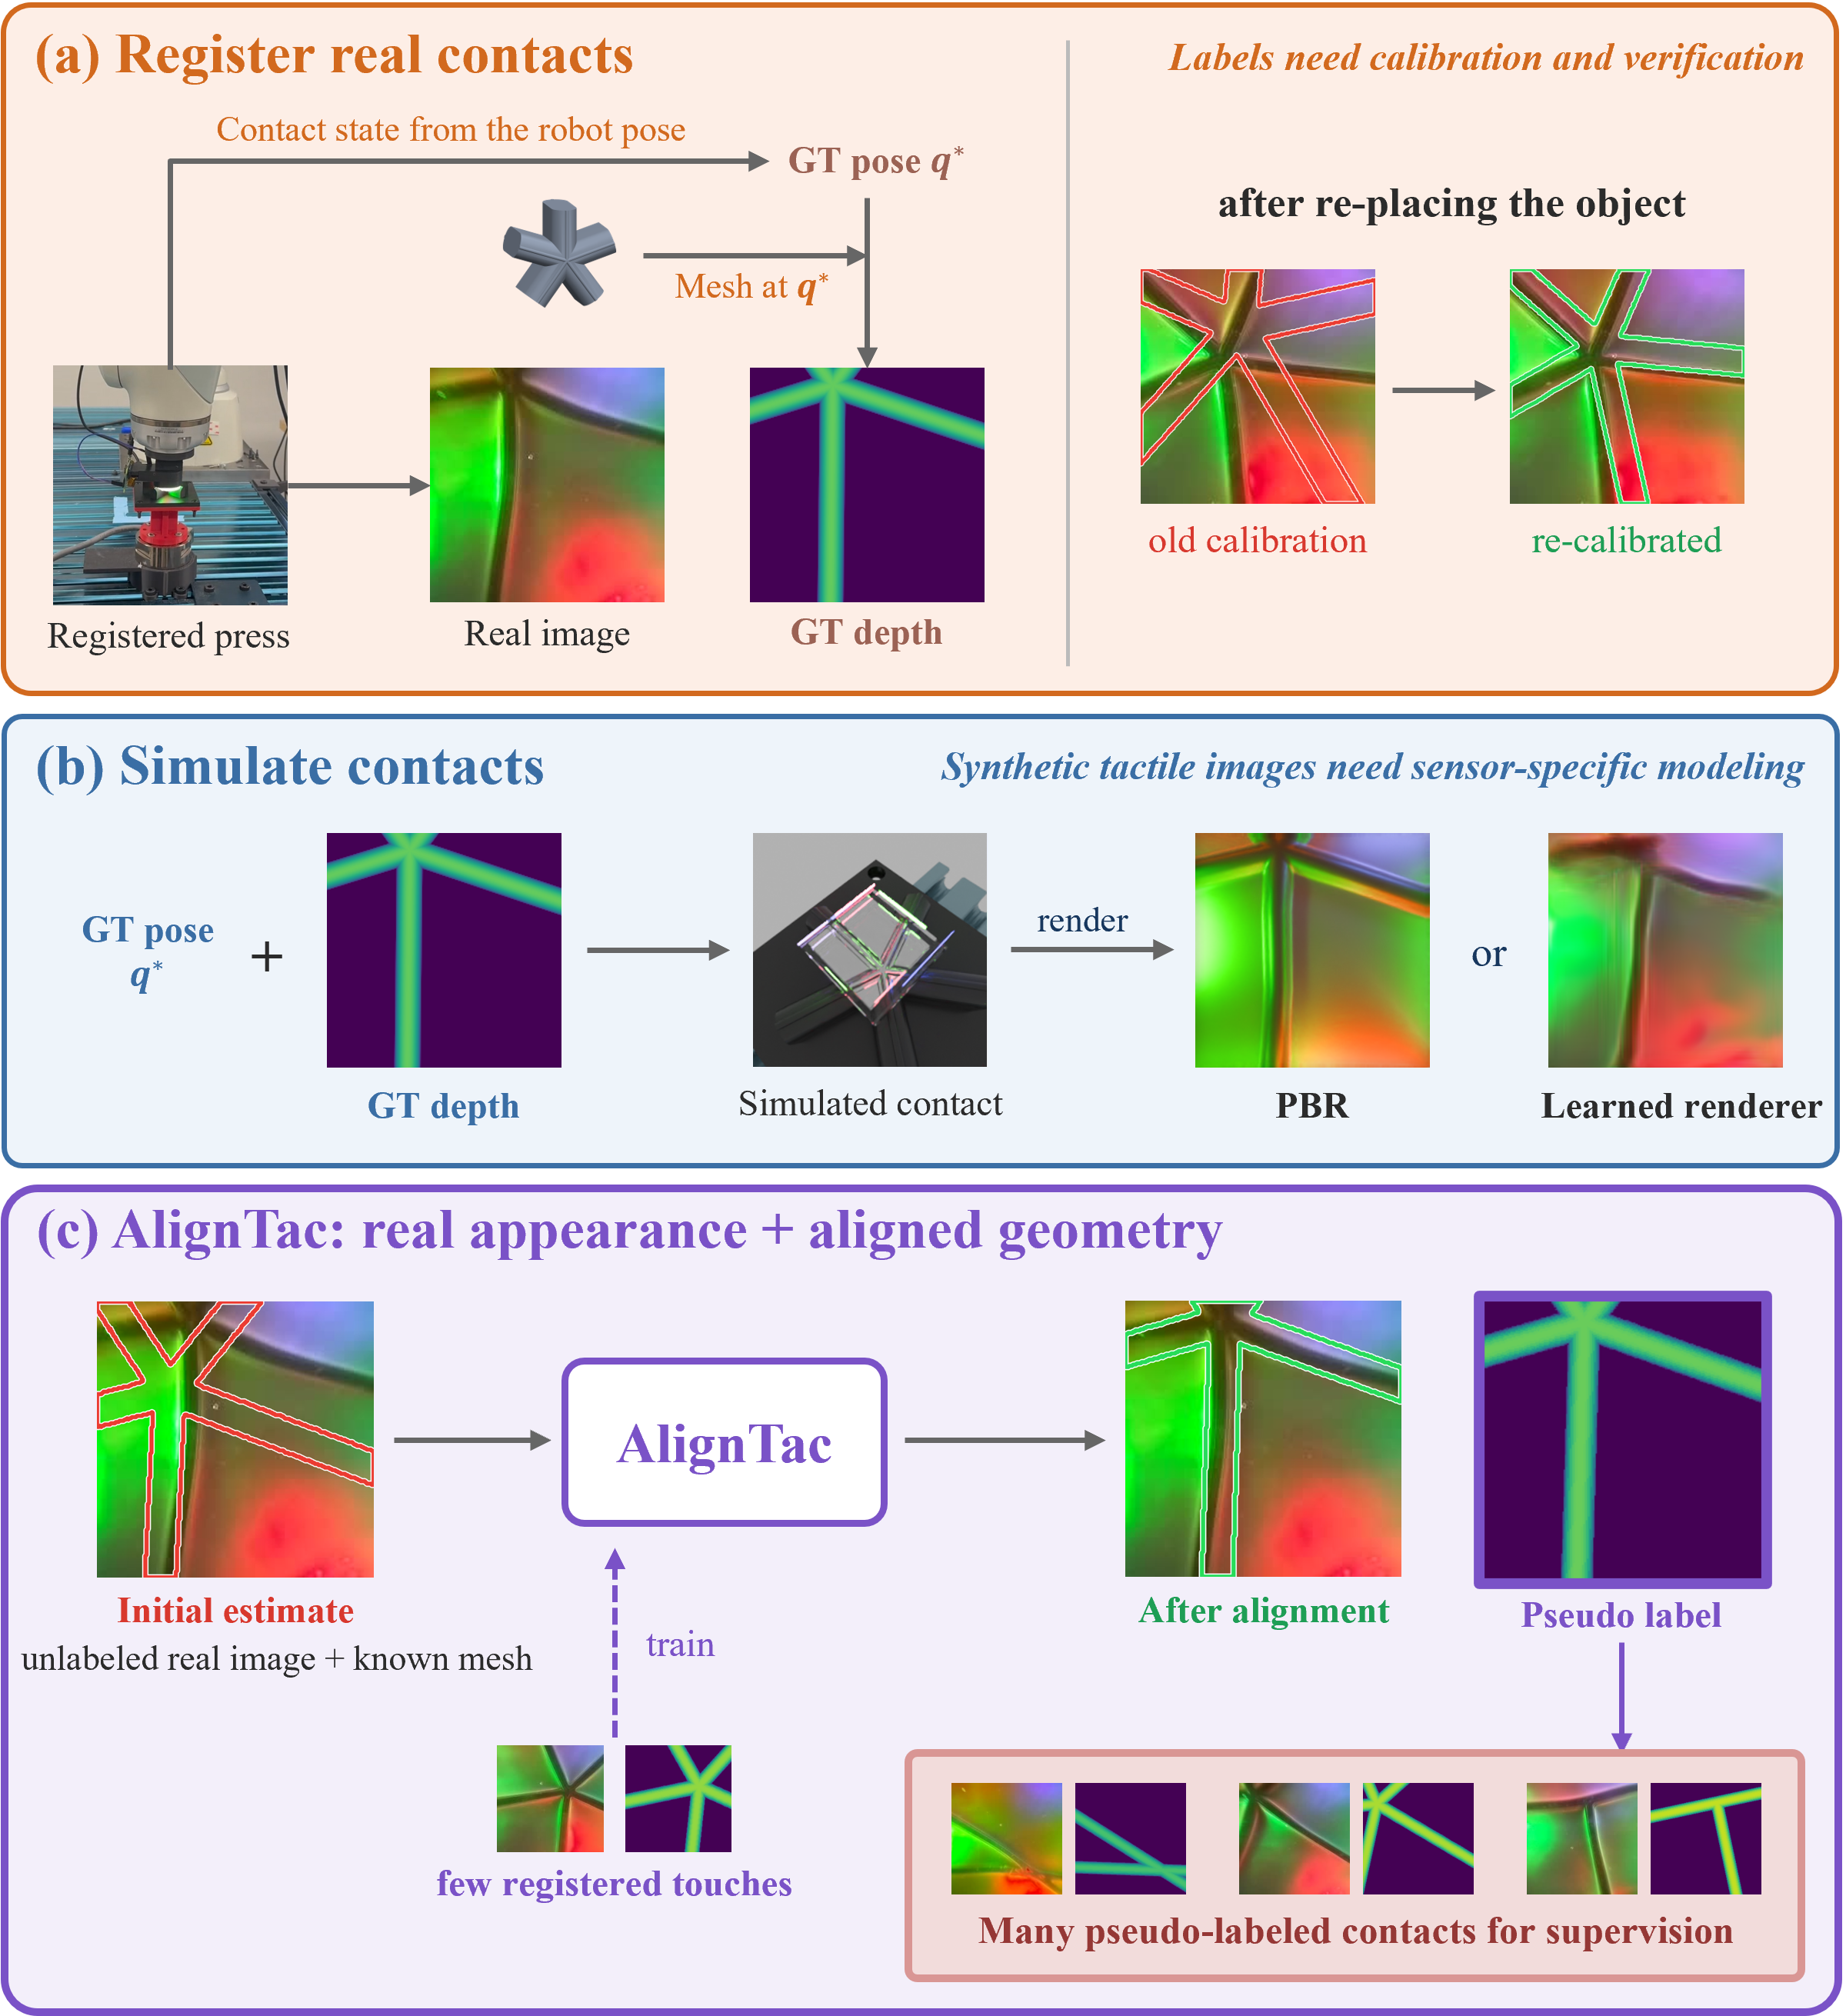
\includegraphics[width=\columnwidth]{figures/intro_figure/AlignTac_Fig1.png}
    \caption{\textbf{From registered labels to aligned geometric supervision.}
    (a) A real contact is labeled by projecting the object mesh at the contact state $q^\ast$ obtained from the robot pose; this needs calibration and verification, repeated after the object is re-placed (right; outlines mark the mesh contact region).
    (b) In simulation the state and depth are given, but tactile images need sensor-specific modeling: a physically based renderer (PBR) or a learned renderer fitted on registered real pairs.
    (c) AlignTac learns from a few registered contacts to align the known mesh with an unlabeled real image, turning the initial estimate into a pseudo-label; the bottom row shows pseudo-labeled contacts of other objects.}
    \label{fig:aligntac_teaser}
\end{figure}

Tactile perception provides robots with contact feedback for dexterous manipulation and physical interaction. Vision-based tactile sensors such as GelSight, GelSlim and DIGIT~\cite{yuan2017gelsight,donlon2018gelslim,lambeta2020digit} use a soft elastomer membrane to convert fine contact-induced deformations into high-resolution visual signals. Learning to recover contact geometry and pose supports perception through touch, but requires scalable, accurately labeled data. A known object mesh can supply these labels only after its contact state is registered to the image.

As shown in Fig.~\ref{fig:aligntac_teaser}a, real data collection requires each labeled contact to be registered. Submillimeter image--geometry accuracy depends on calibration across the robot, sensor and object frames. Systematic kinematic errors can bias the estimated contact state, including on Franka manipulators~\cite{franzese2025mukca}, while sensor mounting and object placement introduce additional uncertainty. A recorded robot pose thus becomes a label only after calibration and verification, repeated whenever the sensor configuration or object placement changes: tactile images are easier to collect than registered labels.

\begin{figure*}[t]
    \centering
    \resizebox{\textwidth}{!}{\input{figures/pipeline.tex}}
    \caption{\textbf{AlignTac training and inference.} (a) Registered contacts train teacher $\Teacher$ and aligner $\Aligner$. The upper branch trains $\Aligner$ from the real image and mesh depth at $q^\ast+\delta$, using correction target $-\delta$. The lower branch refines teacher-initialized states of unlabeled contacts. The aligned state $q_T$ and mesh $\Mesh$ yield depth, normal and planar-pose targets through $\Targets(\Mesh,q_T)$. Student $\Student$ learns from registered and pseudo-labeled real images. (b) Standard prediction uses the image and object identity; mesh-assisted pose refinement is \FinalLine{optional. Thumbnails show a real contact; pose and perturbation glyphs are schematic.}}
    \label{fig:mapl}
\end{figure*}

Simulation and self-training offer two ways to use a small labeled set. Simulation provides geometric targets from known meshes~\cite{wang2022tacto,si2022taxim,chen2023tacchi} (see Fig.~\ref{fig:aligntac_teaser}b), while a renderer must reproduce tactile appearance: illumination, surface reflectance and contact-induced deformation jointly determine the image~\cite{si2022taxim,agarwal2021simulation}. Sensor-specific calibration or fitting on real image--geometry pairs adapts the renderer's appearance; the labeled pairs used for fitting also consume the registration budget. Self-training instead uses a predictor's outputs to label remaining real images and can propagate its errors~\cite{arazo2020pseudo}.

As illustrated in Fig.~\ref{fig:aligntac_teaser}c, our AlignTac combines real tactile appearance with known simulated geometry through contact-state alignment. For a known object, its mesh specifies the geometry, but dense labels depend on a low-dimensional contact state: in-plane rotation, translation and indentation. Obtaining this state for an unlabeled image is difficult: thin contact features make dense labels sensitive to small state errors, mesh depth cannot be compared with tactile RGB directly, and only the few registered contacts are available to learn the correspondence. AlignTac therefore learns the contact-state correction that aligns mesh projections with real tactile observations.

AlignTac learns this alignment from a small registered set (Fig.~\ref{fig:mapl}). We perturb each contact's mesh state while keeping its real image fixed, and train a residual aligner to recover the registered state. For additional real contacts, teacher $\Teacher$ provides the initial state, the aligner corrects it using the observed image, and the aligned geometry supplies depth, normal and planar-pose pseudo-labels. A student $\Student$ learns from these labels and predicts directly from \FinalLine{the tactile image and object identity.}

We evaluate AlignTac against self-training and synthetic augmentation on two GelSlim~4.0 variants: marker-free (sensor A) and dot-marker (sensor B). Experiments use limited real-label budgets. Our contributions are:
\begin{itemize}
    \item A real-image--geometry alignment framework that learns state corrections from perturbations of a small registered set and generates dense geometry and pose \FinalLine{supervision using real tactile images.}
    \item An alignment ablation showing gains in pseudo-label quality and student accuracy, with label efficiency on both sensor variants.
    \item A second-session study in which images captured after object re-placement are labeled by the same aligner, without re-registration.
    \item A matched-budget renderer study identifying complementary benefits of tactile RGB simulation for held-out-object pose coverage and session changes, while accounting for the real labels used to fit the renderer.
\end{itemize}

\section{Related Work}

\noindent\textbf{Tactile simulation and transfer.}
TACTO~\cite{wang2022tacto}, Taxim~\cite{si2022taxim}, Tacchi~\cite{chen2023tacchi} and physics-based rendering~\cite{agarwal2021simulation} model tactile images through optical response and contact geometry or deformation. Differentiable~\cite{xu2022efficient} and GPU-based~\cite{akinola2025tacsl} simulation support learning and control. Transfer methods translate tactile appearance~\cite{chen2022cyclegan}, map real images to simulated depth~\cite{church2022tactile}, or generate tactile images from visual RGB-D~\cite{zhong2025tactgen}. Our study concerns depth-to-RGB renderers fitted on real contact pairs and counts those pairs in the training-label budget.

\noindent\textbf{Tactile geometry reconstruction.}
Prior work learns local contact shape or elastomer deformation directly from tactile images~\cite{bauza2019tactile,zhu2022volumetric}; MeshTac instead reduces the real geometric labels needed to train such predictors.

\noindent\textbf{Tactile representations.}
Pretrained encoders such as SITR, T3 and Sparsh~\cite{gupta2025sitr,zhao2024transferable,higuera2024sparsh} reduce feature learning from scratch; all our predictors share a frozen SITR backbone, and MeshTac addresses supervision rather than the encoder.

\noindent\textbf{Pseudo-labeling and pose refinement.}
Self-training uses model predictions as labels~\cite{lee2013pseudo,xie2020noisy} and can reinforce teacher errors~\cite{arazo2020pseudo}. Known geometry offers an additional constraint. DeepIM~\cite{li2018deepim} learns iterative pose corrections from observed and rendered images; Self6D~\cite{wang2020self6d} uses differentiable rendering to supervise pose on unlabeled RGB-D images. Tac2Pose~\cite{bauza2023tac2pose} estimates pose from a single touch by matching the observed contact shape to simulated contacts of a known mesh. Unlike refinement methods that improve the state estimate at inference, MeshTac learns state corrections from a few registered contacts to generate dense geometry and pose supervision for additional real images; mesh-assisted inference is optional.

\section{Mesh-Aligned Pseudo-Labeling}
\label{sec:mapl}

\begin{figure}[t]
    \centering
    \begin{tikzpicture}[font=\scriptsize, node distance=2.5mm and 3mm,
        box/.style={draw, rounded corners=1pt, align=center, inner sep=2pt, minimum height=5mm, fill=white},
        data/.style={box, fill=black!5}, model/.style={box, fill=blue!8}, rend/.style={box, fill=orange!12},
        arr/.style={-{Latex[length=1.5mm]}, thick}]
        \node[data, text width=31mm] (lab) {$\Kreal$ labeled frames per object (depth, pose)};
        \node[data, text width=26mm, right=of lab] (mesh) {object meshes};
        \node[model, text width=31mm, below=of lab] (f0) {teacher $f_0$ ($\Kreal$-shot model)};
        \node[rend, text width=26mm, below=of mesh] (al) {aligner $A$: (frame, mesh depth at pose) $\to$ pose correction};
        \node[data, text width=31mm, below=4.5mm of f0] (unl) {unlabeled frames $U$};
        \node[box, text width=26mm, right=of unl] (rc) {\textbf{align}: iterate $A$ from the teacher pose};
        \node[model, text width=31mm, below=of unl] (f1) {student $f_1$: $\Kreal$ labeled + aligned $U$};
        \node[box, text width=26mm, below=of rc] (lbl) {\textbf{label}: mesh depth, normals and pose at the aligned pose};
        \draw[arr] (lab) -- (f0); \draw[arr] (lab) -- (al); \draw[arr] (mesh) -- (al);
        \draw[arr] (f0) -- node[left, xshift=-1pt] {pose} (unl); \draw[arr] (unl) -- (rc); \draw[arr] (al) -- (rc);
        \draw[arr] (rc) -- (lbl); \draw[arr] (lbl) -- (f1);
    \end{tikzpicture}
    \caption{\textbf{Mesh-aligned pseudo-labeling.} The $\Kreal$-shot teacher proposes a pose for every unlabeled frame. An aligner trained on the same $\Kreal$ labeled frames iteratively corrects that pose until the object mesh matches the frame; the mesh at the aligned pose, not the teacher's prediction, labels the frame for the student.}
    \label{fig:mapl}
\end{figure}

\begin{figure}[t]
    \centering
    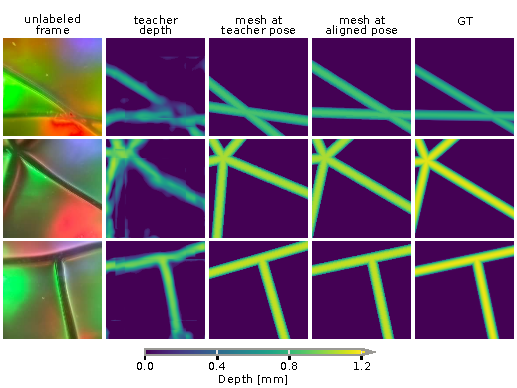
\includegraphics[width=\columnwidth]{figures/fig_align.pdf}
    \caption{\textbf{Labels of unlabeled frames} ($\Kreal=25$; each object's median-quality frame). The teacher's depth is blurred and its pose is off by several degrees; after alignment the mesh label is close to the withheld reference.}
    \label{fig:align}
\end{figure}

\noindent\textbf{Idea.} Let $d(M,q)$ be the depth map of mesh $M$ at contact state $q=(\theta,x,y,z)$ (planar pose and indentation). The reference label of a real frame $I$ of object $M$ is $d(M,q^\ast)$ for the pose $q^\ast$ at which it was captured, so labeling an unlabeled frame is a pose-estimation problem with only four unknowns, and its solution yields depth, normals and pose at once. A $\Kreal$-shot model estimates $q$ only to a few degrees and its dense output is blurred (Fig.~\ref{fig:align}); with the true pose, in contrast, the mesh label is essentially exact (contact IoU $0.95$ against the reference). MAPL closes this gap with a learned refinement.

\noindent\textbf{Residual aligner.} The aligner $A$ is a ResNet-18 (ImageNet-initialized) that takes the real frame and, as a fourth channel, the mesh depth at a candidate pose, and regresses the correction that brings the candidate onto the frame:
\begin{equation}
    A\big(I,\; d(M,q)\big) \;\approx\; q^\ast - q .
\end{equation}
It needs no label beyond the $\Kreal$ frames, because each labeled frame provides unlimited training pairs: we perturb its true pose by up to $\pm8^\circ$, $\pm1.5\,$mm in the plane and $\pm0.15\,$mm of indentation (half of the samples at $0.3\times$ that range, for fine corrections), render the mesh depth at the perturbed pose, and regress the perturbation with a smooth-L1 loss (8k steps, batch 64, AdamW, $3\times10^{-4}$). This is render-and-compare pose refinement~\cite{li2018deepim} with the mesh depth as the ``render'': no photorealistic renderer is involved.

\noindent\textbf{Labeling.} For every unlabeled training frame the teacher $f_0$ (the model trained on the $\Kreal$ labeled frames and GAN-$\Kreal$ data) predicts a pose; the indentation is initialized with the maximum of its predicted depth. The aligner is applied six times, $q\leftarrow q+A(I,d(M,q))$, and the frame receives $d(M,q)$, its normals and $q$ as labels. Every frame is used; no confidence filtering is needed (Sec.~\ref{sec:ablation}). The object of each frame is assumed known, as it is when a user collects frames object by object.

\noindent\textbf{Student.} The student $f_1$ is trained like any other model in this paper on the $\Kreal$ labeled frames, the aligned frames and synthetic frames, with full depth, normal and pose supervision. Following the $\Kreal$-shot rule, the synthetic frames come from the learned renderer retrained on the $\Kreal$ true plus the aligned (depth, image) pairs, which also makes it the most faithful leakage-free renderer of our study (contact-region image error $-13$ to $-19\%$ at every $\Kreal$); the student's accuracy, however, does not depend on this choice (Table~\ref{tab:abl}).

\noindent\textbf{Test-time alignment.} Planar pose is defined with respect to a known object, so the same aligner can also refine the pose a model predicts on a \emph{test} frame (Sec.~\ref{sec:tta}).

\noindent\textbf{Cost and scope.} MAPL adds no labels and leaves the downstream architecture unchanged; it uses the unlabeled frames and the meshes that simulation already requires. Validation and test frames are never pseudo-labeled and never seen by the aligner.

\section{Experimental Setup}
\label{sec:setup}

\noindent\textbf{Sensors and data.} Sensor A is a GelSlim-type fingertip with a $17.5\,$mm gel view and six colored LED emitters. A robot presses it against 12 ridge-pattern objects with known geometry. Ground-truth (GT) depth and normals are mesh projections at the recorded pose, rather than measurements of membrane deformation. After filtering, $4{,}669$ frames remain; every tenth frame is assigned to the validation split ($472$ frames). A second session, recorded on another day after the objects were re-placed, contains $854$ reviewed test frames from 11 objects. Their poses are re-estimated from contact masks. Sensor B, \sensorB{}~\cite{sipos2024gelslim4}, has a marker array, different illumination and a $12\,$mm view. We use its public dataset of the same 12 objects ($1{,}620$ test frames). We re-register its clipped, smoothed depth labels to the meshes by pose fitting ($0.018\,$mm mean residual) and use the resulting targets for every sensor-B method.

\noindent\textbf{Label budget.} Each object contributes $\Kreal\in\{10,25,50,100\}$ evenly spaced labeled training frames. The teacher, renderer and aligner share these frames, which represent $3\%$, $7\%$, $14\%$ and $29\%$ of the sensor-A training set. All other training images are available without labels. Our primary setting is $K\le25$; the larger budgets show how performance changes as more labels become available. Validation and test images are excluded from component training. Validation labels are used for checkpoint selection and are not included in the stated training-label budget.

\noindent\textbf{Models and training.} All methods use a frozen SITR-B/18 encoder~\cite{gupta2025sitr}, a DPT decoder~\cite{ranftl2021dpt} for depth and normals, and a planar-pose MLP ($12$M trainable parameters). We train the main sensor-A models for 150 epochs and use 50 epochs for ablations, three-seed checks and sensor B. Aligner perturbations span $\pm8^\circ$, $\pm1.5\,$mm in-plane and $\pm0.15\,$mm in indentation; half use ranges scaled by $0.3$. Training uses smooth L1 for 8,000 steps (batch 64, AdamW, learning rate $3\times10^{-4}$). Main sensor-A batches mix 24 real and 40 synthetic examples; renderer-free and sensor-B aligners use real examples only. The main sensor-A teacher uses the $K$ real frames and learned-renderer data, whereas the other two use a real-only teacher. The sensor-A student additionally uses synthetic images from a renderer retrained on labeled and aligned pairs.

\noindent\textbf{Renderers and cost.} The physical renderer uses Blender/Cycles with illumination fitted to a no-contact image and manually tuned contact parameters. The learned renderer maps depth to RGB with a pix2pix network~\cite{isola2017pix2pix}. Both use the same $5{,}345$ simulated contacts. An additional \emph{leaky renderer} reference uses all $4{,}197$ real training pairs: it exceeds $K$ but does not include validation frames. In the held-out-object study, it also includes real data from the evaluation objects. On one RTX 6000 Ada GPU, aligner training takes about $20$ minutes, pseudo-labeling $0.5\,$s per frame, and student training $1.3$ hours for 50 epochs or $2.2$ hours for 150.

\noindent\textbf{Metrics.} We report all-pixel depth MSE (mm$^2$), contact MAE within the GT contact region (depth $>0$; mm), contact IoU (predicted depth $>0.05\,$mm versus GT depth $>0$), and mean rotation error (deg). Because roughly $90\%$ of the pixels are background, contact MAE and IoU expose errors that all-pixel MSE can obscure. Dense metrics use the checkpoint with the lowest validation depth MSE; sensor-A pose metrics use the checkpoint with the lowest validation rotation error.

\section{Experiments}
\label{sec:exp}

\begin{figure*}[t]
    \centering
    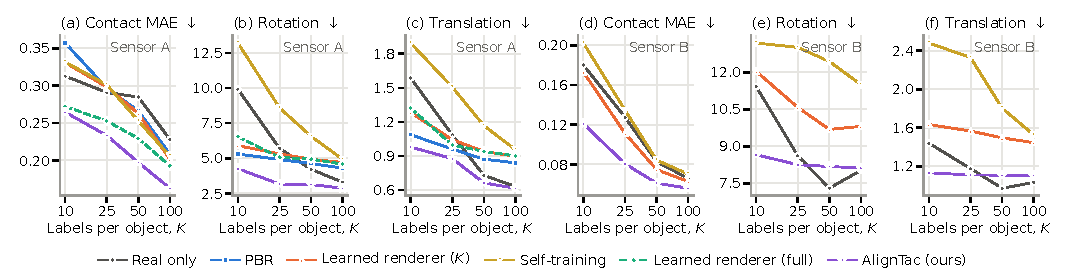
\includegraphics[width=0.9\textwidth]{figures/fig_kshot.pdf}
    \caption{\textbf{Label efficiency on two tactile sensors.} $K$: labeled training contacts per object. (a--c) Sensor-A validation, 150 epochs; the all-pairs (leaky) reference uses extra real labels and 50 epochs at $K=10$. (d--f) Sensor-B test, 50 epochs, renderer-free MeshTac. Matched methods share the registered contacts.}
    \label{fig:kshot}
\end{figure*}

\begin{table}[!htb]
\centering
\tableformat
\setlength{\tabcolsep}{3.0pt}
\begin{tabularx}{\columnwidth}{@{}rXrrrr@{}}
\toprule
$\Kreal$ & Method & \metrichead{Depth}{MSE} & \metrichead{Contact}{MAE} & \shortstack[c]{\strut IoU\\\strut $\uparrow$} & \metrichead{Rot.}{(deg)} \\
\midrule
\tabkshotshort
\bottomrule
\end{tabularx}
\caption{\textbf{Label-budget comparison on sensor A.} Validation: $472$ frames; $K$ labels per object. Self-training and MeshTac also use unlabeled images. Italic all-pairs rows exceed the budget ($K=10$: 50 epochs; others: 150). Matched rows use 150 epochs; bold marks the best at each $K$.}
\label{tab:kshot}
\end{table}

\subsection{Label Efficiency}
\label{sec:kshot}
We compare real-only training, learned-renderer augmentation, teacher-depth self-training and MeshTac using the same registered contacts at each $K$ (Table~\ref{tab:kshot}, Fig.~\ref{fig:kshot}). Self-training and MeshTac receive the same unlabeled training images; self-training applies pose supervision only to the registered subset.

At $K=25$, MeshTac lowers depth MSE by $19\%$ and contact MAE by $20\%$ relative to real-only training. Synthetic augmentation slightly improves all-pixel MSE but worsens contact MAE and IoU: lower MSE need not mean better contact reconstruction when background pixels dominate. Three-seed comparisons at 50 epochs confirm the MeshTac gain. MeshTac at $K=50$ also outperforms real-only training at $K=100$ in depth MSE ($0.0307$ versus $0.0369$), showing the value of aligned contacts beyond the registered set.

Removing the renderer preserves the depth improvement at every budget, supporting alignment as the main source of the within-session gain. Synthetic augmentation becomes useful for contact reconstruction at $K\ge50$ and under session changes (Sec.~\ref{sec:general}). Rotation improves for $K\le50$ but not at $K=100$; the reconstruction gain does not extend uniformly to pose.

\begin{table}[!htb]
\centering
\tableformat
\setlength{\tabcolsep}{1.8pt}
\resizebox{\columnwidth}{!}{%
\begin{tabular}{@{}lrrrrrrr@{}}
\toprule
& \multicolumn{3}{c}{Pseudo-labels vs.\ GT} & \multicolumn{4}{c}{Student validation} \\
\cmidrule(lr){2-4}\cmidrule(lr){5-8}
Pseudo-label & \shortstack[c]{\strut IoU\\\strut $\uparrow$} & \metrichead{Cont.}{MAE} & \metrichead{Rot.}{(deg)} & \metrichead{Depth}{MSE} & \metrichead{Cont.}{MAE} & \shortstack[c]{\strut IoU\\\strut $\uparrow$} & \metrichead{Rot.}{(deg)} \\
\midrule
\tabrcablmain
\bottomrule
\end{tabular}}
\caption{\textbf{Pseudo-label quality and student performance.} Sensor A, $K=25$, 50 epochs. Student results are three-seed means except \emph{Teacher depth + pose}. Withheld training GT scores labels only. $^{1/2}$ uses mesh depth for each object's half with lowest render error, teacher depth otherwise, and L1-search pose throughout. $\ddagger$ removes the renderer throughout the pipeline.}
\label{tab:abl}
\end{table}

\begin{figure}[t]
    \centering
    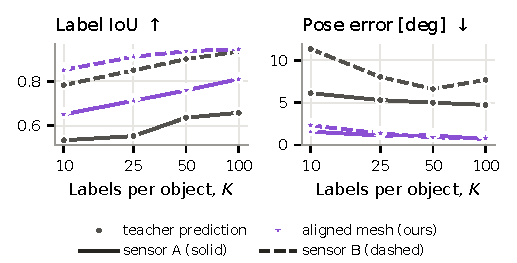
\includegraphics[width=\columnwidth]{figures/fig_labels.pdf}
    \caption{\textbf{Teacher and aligned-mesh label quality.} IoU, contact MAE and rotation error on unlabeled training images from both sensors, across label budgets $K$. Withheld GT is used only to evaluate the labels.}
    \label{fig:labels}
\end{figure}

\subsection{Ablation Study on Alignment Quality}
\label{sec:ablation}
We label the same unlabeled images with teacher predictions, L1 render-and-compare search or learned alignment, then evaluate both label quality and the student trained on those targets (Table~\ref{tab:abl}). Adding teacher pose isolates pose supervision; the renderer-free row additionally removes synthetic data.

Adding teacher pose mainly improves student rotation. Learned alignment improves label quality on both sensors (Fig.~\ref{fig:labels}) and raises student IoU from $0.624$ to $0.729$ relative to teacher-depth self-training. Correcting mesh placement therefore improves the supervision supplied to the student.

L1 search gives smaller gains. At $K=25$, the renderer assigns lower image error to the search-selected pose than to the GT pose on $93\%$ of frames. Thus, image similarity can favor a geometrically incorrect state; this statistic measures candidate ranking, not the search's pose-failure rate.

Gains persist with varied aligner settings and two random label selections; a second labeling round adds little. At $K=25$, $1.6\%$ of aligned sensor-A training poses exceed $5^\circ$ error, mostly on one nearly symmetric object. Translation errors follow repeated ridges, where different states can yield similar contact geometry.

\begin{figure*}[t]
    \centering
    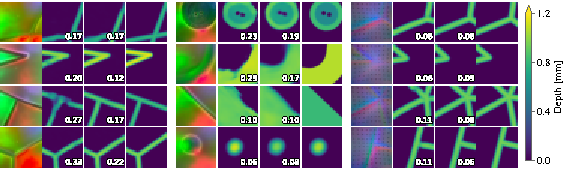
\includegraphics[width=0.8\textwidth]{figures/fig_qual.pdf}
    \caption{\textbf{Contact-depth reconstruction at $K=25$.} Each sensor shows three objects; each frame has its object's median contact-MAE improvement over real-only training. Numbers are contact MAE (mm), and depth maps share a color scale. Both displayed MeshTac models use synthetic data; the sensor-B curves in Fig.~\ref{fig:kshot}d--f use the renderer-free variant.}
    \label{fig:qual}
\end{figure*}

\begin{table}[!htb]
\centering
\tableformat
\setlength{\tabcolsep}{3pt}
\begin{tabularx}{\columnwidth}{@{}rXrr@{}}
\toprule
\multicolumn{4}{l}{\textbf{Sensor A: second-session evaluation}} \\
$\Kreal$ & Method & \metrichead{Contact}{MAE} & \shortstack[c]{\strut IoU\\\strut $\uparrow$} \\
\midrule
\tabcrossshortb
\midrule\midrule
\multicolumn{4}{l}{\textbf{Sensor B: sensor-specific training}} \\
$\Kreal$ & Method & \metrichead{Contact}{MAE} & \shortstack[c]{\strut IoU\\\strut $\uparrow$} \\
\midrule
\tabsbshortb
\bottomrule
\end{tabularx}
\caption{\textbf{Second-session and second-sensor results.} Top: sensor-A models tested on session 2 without retraining ($854$ frames). $\dagger$ uses all training labels from nine objects, with different object coverage from the $K$-shot rows. Bottom: models trained on sensor B and evaluated on its test set ($1{,}620$ frames); MeshTac is renderer-free. Sensor-B values are three-seed mean $\pm$ standard deviation. Contact MAE is in mm.}
\label{tab:general}
\end{table}

\subsection{Generalization Across Sessions and Sensors}
\label{sec:general}
\noindent\textbf{Second session.} We test sensor-A models on another day's contacts after object re-placement, without retraining (Table~\ref{tab:general}, top). MeshTac lowers contact MAE by $16\%$ at $K=25$ and $28\%$ at $K=100$ relative to real-only training. At $K=100$, synthetic augmentation improves on renderer-free MeshTac, which still outperforms self-training. At $K=25$, removing it gives slightly lower MAE ($0.306$ versus $0.310$). The benefit of simulation under this session change thus depends on the label budget.

\noindent\textbf{Second sensor.} We train each method separately on sensor B, keeping the aligner settings unchanged (Table~\ref{tab:general}, bottom). Renderer-free MeshTac lowers contact MAE by $36\%$ at $K=25$ and matches real-only training with twice as many labels. Three-seed checks at every budget support the gain, and evaluation with the original public labels gives the same qualitative result. At the other budgets, MeshTac lowers contact MAE by $15$--$33\%$, compared with at most $10\%$ from learned-renderer augmentation and no gain from self-training (Fig.~\ref{fig:kshot}e).

Figure~\ref{fig:qual} illustrates differences in ridge continuity and junction placement; quantitative comparisons use all evaluation frames.

\begin{table}[!htb]
\centering
\tableformat
\setlength{\tabcolsep}{3.5pt}
\begin{tabular}{@{}rrrrrrrrr@{}}
\toprule
& \multicolumn{4}{c}{Validation (session 1)} & \multicolumn{4}{c}{Session 2} \\
\cmidrule(lr){2-5}\cmidrule(lr){6-9}
& \multicolumn{2}{c}{Real only} & \multicolumn{2}{c}{MeshTac} & \multicolumn{2}{c}{Real only} & \multicolumn{2}{c}{MeshTac} \\
$\Kreal$ & pred. & +align & pred. & +align & pred. & +align & pred. & +align \\
\midrule
\tabposeref
\bottomrule
\end{tabular}
\caption{\textbf{Rotation error before and after mesh-assisted refinement.} Sensor A, mean error (deg) on session-1 validation and session-2 test images. \emph{pred.}: predictor output; \emph{+align}: six fixed-aligner iterations, without retraining.}
\label{tab:poseref}
\end{table}

\subsection{Mesh-Assisted Test-Time Pose Refinement}
\label{sec:tta}
We apply six fixed-aligner updates to real-only and MeshTac predictions using the test image and known mesh (Table~\ref{tab:poseref}). At $K\ge25$, both initializations reach $0.4$--$1.2^\circ$ mean rotation error within session 1: the aligner remains useful after student training and with a different predictor. At these budgets, session-2 means near $5^\circ$ exceed medians of $1.5$--$1.8^\circ$, motivating a confidence estimate to detect large residual errors.

\begin{table}[!htb]
\centering
\tableformat
\begin{tabularx}{\columnwidth}{Xrrrr}
\toprule
Method & \metrichead{Depth}{MSE} & \metrichead{Contact}{MAE} & \shortstack[c]{\strut IoU\\\strut $\uparrow$} & \metrichead{Rot.}{(deg)} \\
\midrule
\tabloomain
\bottomrule
\end{tabularx}
\caption{\textbf{Renderer baselines on held-out objects.} Sensor A, $1{,}244$ frames from three objects. Matched methods exclude their real contacts from training; simulation can use their meshes, except in the \emph{w/o held-out meshes} control. The italic leaky reference also uses real training pairs from these objects. Bold marks the best matched result.}
\label{tab:loo}
\end{table}

\subsection{Renderer Baselines: Unseen Objects and Label Leakage}
\label{sec:study}
We remove three objects from real training while allowing simulation to use their meshes (Table~\ref{tab:loo}). A control excludes those meshes as well. Simulated contacts lower rotation error from $64.7^\circ$ to $5$--$7^\circ$; removing the held-out meshes largely removes this gain. Dense MSE improves by at most $13\%$ among matched methods. In this setting, simulation provides more effective supervision for unseen-object pose than for dense reconstruction.

We then compare renderers trained on the same $K$ registered contacts with the all-pairs reference. The latter lowers MSE by $24$--$26\%$ in the few-label regime, but has access to additional real training labels. It represents a larger supervision budget; validation images remain excluded. Across 14 matched settings, contact-region image L1 correlates with downstream MSE ($\rho=0.95$). This supports its use for screening renderers, although the pooled correlation across budgets and variants does not establish causality or replace downstream evaluation.

\section{Discussion and Conclusion}

\noindent\textbf{Main findings.} MeshTac turns unlabeled real contacts into geometric supervision by aligning a known object mesh to each image. The ablations connect the improvement to the quality of this alignment: refining the contact state improves the projected labels, and the student trained on those labels reconstructs contact more accurately. Because the gain remains when synthetic images are removed, the evidence points to contact-state error---rather than appearance synthesis alone---as the main obstacle to using unlabeled contacts within a capture session.

\noindent\textbf{Lessons for label-efficient tactile learning.} Geometry coverage and sensor appearance play different roles. Real unlabeled images already provide the target appearance, so mesh alignment is a strong first step when registered contacts are scarce. Synthetic data becomes more useful when coverage changes, as seen in the second session and the unseen-object pose study. This suggests a practical order of operations: first establish a renderer-free alignment baseline, then add simulation when pose coverage or session robustness is limiting. Comparisons should disclose the real data used by the renderer, teacher and aligner, together with validation labels used for checkpoint selection; otherwise renderer supervision can be mistaken for a gain from simulation. Image fidelity can screen renderers, but downstream contact metrics remain necessary because lower all-pixel error need not mean better contact localization.

\noindent\textbf{Limitations and future work.} MeshTac assumes known objects: the predictor uses object identity, while pseudo-labeling and optional refinement require a mesh. The targets are mesh projections, so the experiments measure registered object geometry rather than physical elastomer deformation. The 12 ridge-pattern objects, labeled validation set and quasi-static presses leave curved and textured contacts, unknown objects, shear and slip untested. Repeated ridges also create translation ambiguity, and a small set of cross-session alignments retain large errors. Future work should develop uncertainty-aware or symmetry-aware alignment, extend the labels to dynamic contact, and test whether the geometric gains improve closed-loop manipulation. Relaxing the known-mesh assumption through joint shape and contact-state estimation is a further direction.


% The shorter sentence-case captions allow all table floats before the
% bibliography page; flushend can balance the final text columns normally.
\bibliographystyle{IEEEtran}
\bibliography{refs}

\end{document}
 for an author copy.
\ifdefined\AlignTacAuthorVersion
\author{I-Hsuan Huang$^{*}$, Xiaohao Xu$^{*}$, Xiangdong Wang, Xiaonan Huang, and Nima Fazeli%
\thanks{$^{*}$Equal contribution. All authors are with the University of Michigan, Ann Arbor, MI, USA.
Correspondence: \texttt{\{ihsuan, xiaohaox\}@umich.edu}.}%
}
\else
\author{Anonymous submission}
\fi
\hypersetup{pdfauthor={},pdftitle={AlignTac: Aligning Real Tactile Images with Simulated Geometry for Label-Efficient Learning},pdfsubject={},pdfkeywords={}}

% Final-line typography. No font-size or margin changes.
% Keep selected final phrases together so a paragraph does not end in a short fragment.
\DeclareRobustCommand{\FinalLine}[1]{\mbox{#1}}
\usepackage{etoolbox}
% Bibliography line-break formatting for the included reference entries.
% BibTeX still generates main.bbl normally. Each unchanged entry receives a
% nonbreaking final phrase (last two words tied with ~, 2026-10-25); reference wording and publication data are retained.
% Edited entries fall back to standard text and request a new layout check.
\ExplSyntaxOn
\prop_new:N \g_aligntac_bib_original_prop
\prop_new:N \g_aligntac_bib_formatted_prop
\cs_new_protected:Npn \BibLayoutRecord #1#2#3
  {
    \prop_gput:Nnn \g_aligntac_bib_original_prop {#1}{#2}
    \prop_gput:Nnn \g_aligntac_bib_formatted_prop {#1}{#3}
  }
\cs_new_protected:Npn \AlignTacFormatBib #1#2
  {
    \tl_set:Nn \l_tmpa_tl {#2}
    \tl_trim_spaces:N \l_tmpa_tl
    \prop_get:NnNTF \g_aligntac_bib_original_prop {#1} \l_tmpb_tl
      {
        \tl_if_eq:NNTF \l_tmpa_tl \l_tmpb_tl
          {
            \prop_get:NnN \g_aligntac_bib_formatted_prop {#1} \l_tmpb_tl
            \tl_use:N \l_tmpb_tl
          }
          {
            \PackageWarning{AlignTac}{Reference~#1~changed;~recheck~its~final~line}
            \tl_use:N \l_tmpa_tl
          }
      }
      {
        \PackageWarning{AlignTac}{New~reference~#1;~recheck~its~final~line}
        \tl_use:N \l_tmpa_tl
      }
  }
\ExplSyntaxOff
\makeatletter
\newcommand{\AlignTacBibSetup}{%
  \let\AlignTacOriginalBibitem\bibitem
  \long\def\bibitem##1##2\par{%
    \AlignTacOriginalBibitem{##1}%
    \begingroup\raggedright
      \AlignTacFormatBib{##1}{##2}\par
    \endgroup\ignorespaces}%
}
\apptocmd{\thebibliography}{\AlignTacBibSetup}{}%
 {\PackageError{AlignTac}{Unable to install bibliography layout}{Use the supplied ieeeconf class.}}
\makeatother
\BibLayoutRecord{yuan2017gelsight}{W.~Yuan, S.~Dong, and E.~H. Adelson, ``{GelSight}: High-resolution robot tactile sensors for estimating geometry and force,'' \emph{Sensors}, vol.~17, no.~12, 2017.}{W.~Yuan, S.~Dong, and E.~H. Adelson, ``{GelSight}: High-resolution robot tactile sensors for estimating geometry and force,'' \emph{Sensors}, vol.~17, no.~12,~2017.}
\BibLayoutRecord{donlon2018gelslim}{E.~Donlon, S.~Dong, M.~Liu, J.~Li, E.~Adelson, and A.~Rodriguez, ``{GelSlim}: A high-resolution, compact, robust, and calibrated tactile-sensing finger,'' in \emph{Proc. IEEE/RSJ Int. Conf. Intelligent Robots and Systems (IROS)}, 2018.}{E.~Donlon, S.~Dong, M.~Liu, J.~Li, E.~Adelson, and A.~Rodriguez, ``{GelSlim}: A high-resolution, compact, robust, and calibrated tactile-sensing finger,'' in \emph{Proc. IEEE/RSJ Int. Conf. Intelligent Robots and Systems (IROS)},~2018.}
\BibLayoutRecord{lambeta2020digit}{M.~Lambeta, P.-W. Chou, S.~Tian, B.~Yang, B.~Maloon, V.~R. Most, D.~Stroud, R.~Santos, A.~Byagowi, G.~Kammerer, D.~Jayaraman, and R.~Calandra, ``{DIGIT}: A novel design for a low-cost compact high-resolution tactile sensor with application to in-hand manipulation,'' \emph{IEEE Robotics and Automation Letters}, vol.~5, no.~3, pp. 3838--3845, 2020.}{M.~Lambeta, P.-W. Chou, S.~Tian, B.~Yang, B.~Maloon, V.~R. Most, D.~Stroud, R.~Santos, A.~Byagowi, G.~Kammerer, D.~Jayaraman, and R.~Calandra, ``{DIGIT}: A novel design for a low-cost compact high-resolution tactile sensor with application to in-hand manipulation,'' \emph{IEEE Robotics and Automation Letters}, vol.~5, no.~3, pp. 3838--3845,~2020.}
\BibLayoutRecord{franzese2025mukca}{G.~Franzese, M.~Spahn, J.~Kober, and C.~Della~Santina, ``{MUKCa}: Accurate and affordable cobot calibration without external measurement devices,'' \emph{arXiv preprint arXiv:2503.12584}, 2025.}{G.~Franzese, M.~Spahn, J.~Kober, and C.~Della~Santina, ``{MUKCa}: Accurate and affordable cobot calibration without external measurement devices,'' \emph{arXiv preprint arXiv:2503.12584},~2025.}
\BibLayoutRecord{wang2022tacto}{S.~Wang, M.~Lambeta, P.-W. Chou, and R.~Calandra, ``{TACTO}: A fast, flexible, and open-source simulator for high-resolution vision-based tactile sensors,'' \emph{IEEE Robotics and Automation Letters}, vol.~7, no.~2, pp. 3930--3937, 2022.}{S.~Wang, M.~Lambeta, P.-W. Chou, and R.~Calandra, ``{TACTO}: A fast, flexible, and open-source simulator for high-resolution vision-based tactile sensors,'' \emph{IEEE Robotics and Automation Letters}, vol.~7, no.~2, pp. 3930--3937,~2022.}
\BibLayoutRecord{si2022taxim}{Z.~Si and W.~Yuan, ``{Taxim}: An example-based simulation model for {GelSight} tactile sensors,'' \emph{IEEE Robotics and Automation Letters}, vol.~7, no.~2, pp. 2361--2368, 2022.}{Z.~Si and W.~Yuan, ``{Taxim}: An example-based simulation model for {GelSight} tactile sensors,'' \emph{IEEE Robotics and Automation Letters}, vol.~7, no.~2, pp. 2361--2368,~2022.}
\BibLayoutRecord{chen2023tacchi}{Z.~Chen, S.~Zhang, S.~Luo, F.~Sun, and B.~Fang, ``{Tacchi}: A pluggable and low computational cost elastomer deformation simulator for optical tactile sensors,'' \emph{IEEE Robotics and Automation Letters}, vol.~8, no.~3, pp. 1239--1246, 2023.}{Z.~Chen, S.~Zhang, S.~Luo, F.~Sun, and B.~Fang, ``{Tacchi}: A pluggable and low computational cost elastomer deformation simulator for optical tactile sensors,'' \emph{IEEE Robotics and Automation Letters}, vol.~8, no.~3, pp. 1239--1246,~2023.}
\BibLayoutRecord{agarwal2021simulation}{A.~Agarwal, T.~Man, and W.~Yuan, ``Simulation of vision-based tactile sensors using physics based rendering,'' in \emph{Proc. IEEE Int. Conf. Robotics and Automation (ICRA)}, 2021, pp. 1--7.}{A.~Agarwal, T.~Man, and W.~Yuan, ``Simulation of vision-based tactile sensors using physics based rendering,'' in \emph{Proc. IEEE Int. Conf. Robotics and Automation (ICRA)}, 2021, pp.~1--7.}
\BibLayoutRecord{arazo2020pseudo}{E.~Arazo, D.~Ortego, P.~Albert, N.~E. O'Connor, and K.~McGuinness, ``Pseudo-labeling and confirmation bias in deep semi-supervised learning,'' in \emph{Proc. Int. Joint Conf. Neural Networks (IJCNN)}, 2020.}{E.~Arazo, D.~Ortego, P.~Albert, N.~E. O'Connor, and K.~McGuinness, ``Pseudo-labeling and confirmation bias in deep semi-supervised learning,'' in \emph{Proc. Int. Joint Conf. Neural Networks (IJCNN)},~2020.}
\BibLayoutRecord{xu2022efficient}{J.~Xu, S.~Kim, T.~Chen, A.~R. Garcia, P.~Agrawal, W.~Matusik, and S.~Sueda, ``Efficient tactile simulation with differentiability for robotic manipulation,'' in \emph{Proc. Conf. Robot Learning (CoRL)}, 2022, pp. 1488--1498.}{J.~Xu, S.~Kim, T.~Chen, A.~R. Garcia, P.~Agrawal, W.~Matusik, and S.~Sueda, ``Efficient tactile simulation with differentiability for robotic manipulation,'' in \emph{Proc. Conf. Robot Learning (CoRL)}, 2022, pp.~1488--1498.}
\BibLayoutRecord{akinola2025tacsl}{I.~Akinola, J.~Xu, J.~Carius, D.~Fox, and Y.~Narang, ``{TacSL}: A library for visuotactile sensor simulation and learning,'' \emph{IEEE Transactions on Robotics}, 2025.}{I.~Akinola, J.~Xu, J.~Carius, D.~Fox, and Y.~Narang, ``{TacSL}: A library for visuotactile sensor simulation and learning,'' \emph{IEEE Transactions on Robotics},~2025.}
\BibLayoutRecord{chen2022cyclegan}{W.~Chen, Y.~Xu, Z.~Chen, P.~Zeng, R.~Dang, R.~Chen, and J.~Xu, ``Bidirectional sim-to-real transfer for {GelSight} tactile sensors with {CycleGAN},'' \emph{IEEE Robotics and Automation Letters}, vol.~7, no.~3, pp. 6187--6194, 2022.}{W.~Chen, Y.~Xu, Z.~Chen, P.~Zeng, R.~Dang, R.~Chen, and J.~Xu, ``Bidirectional sim-to-real transfer for {GelSight} tactile sensors with {CycleGAN},'' \emph{IEEE Robotics and Automation Letters}, vol.~7, no.~3, pp. 6187--6194,~2022.}
\BibLayoutRecord{church2022tactile}{A.~Church, J.~Lloyd, R.~Hadsell, and N.~F. Lepora, ``Tactile sim-to-real policy transfer via real-to-sim image translation,'' in \emph{Proc. Conf. Robot Learning (CoRL)}, 2022, pp. 1645--1654.}{A.~Church, J.~Lloyd, R.~Hadsell, and N.~F. Lepora, ``Tactile sim-to-real policy transfer via real-to-sim image translation,'' in \emph{Proc. Conf. Robot Learning (CoRL)}, 2022, pp.~1645--1654.}
\BibLayoutRecord{zhong2025tactgen}{S.~Zhong, A.~Albini, P.~Maiolino, and I.~Posner, ``{TactGen}: Tactile sensory data generation via zero-shot sim-to-real transfer,'' \emph{IEEE Transactions on Robotics}, vol.~41, pp. 1316--1328, 2025.}{S.~Zhong, A.~Albini, P.~Maiolino, and I.~Posner, ``{TactGen}: Tactile sensory data generation via zero-shot sim-to-real transfer,'' \emph{IEEE Transactions on Robotics}, vol.~41, pp. 1316--1328,~2025.}
\BibLayoutRecord{bauza2019tactile}{M.~Bauza, O.~Canal, and A.~Rodriguez, ``Tactile mapping and localization from high-resolution tactile imprints,'' in \emph{Proc. IEEE Int. Conf. Robotics and Automation (ICRA)}, 2019.}{M.~Bauza, O.~Canal, and A.~Rodriguez, ``Tactile mapping and localization from high-resolution tactile imprints,'' in \emph{Proc. IEEE Int. Conf. Robotics and Automation (ICRA)},~2019.}
\BibLayoutRecord{zhu2022volumetric}{X.~Zhu, S.~Jain, M.~Tomizuka, and J.~van Baar, ``Learning to synthesize volumetric meshes from vision-based tactile imprints,'' in \emph{Proc. IEEE Int. Conf. Robotics and Automation (ICRA)}, 2022.}{X.~Zhu, S.~Jain, M.~Tomizuka, and J.~van Baar, ``Learning to synthesize volumetric meshes from vision-based tactile imprints,'' in \emph{Proc. IEEE Int. Conf. Robotics and Automation (ICRA)},~2022.}
\BibLayoutRecord{gupta2025sitr}{H.~Gupta, Y.~Mo, S.~Jin, and W.~Yuan, ``Sensor-invariant tactile representation,'' in \emph{Proc. Int. Conf. Learning Representations (ICLR)}, 2025.}{H.~Gupta, Y.~Mo, S.~Jin, and W.~Yuan, ``Sensor-invariant tactile representation,'' in \emph{Proc. Int. Conf. Learning Representations (ICLR)},~2025.}
\BibLayoutRecord{zhao2024transferable}{J.~Zhao, Y.~Ma, L.~Wang, and E.~Adelson, ``Transferable tactile transformers for representation learning across diverse sensors and tasks,'' in \emph{Proc. Conf. Robot Learning (CoRL)}, 2024.}{J.~Zhao, Y.~Ma, L.~Wang, and E.~Adelson, ``Transferable tactile transformers for representation learning across diverse sensors and tasks,'' in \emph{Proc. Conf. Robot Learning (CoRL)},~2024.}
\BibLayoutRecord{higuera2024sparsh}{C.~Higuera, A.~Sharma, C.~K. Bodduluri, T.~Fan, P.~Lancaster, M.~Kalakrishnan, M.~Kaess, B.~Boots, M.~Lambeta, T.~Wu, and M.~Mukadam, ``{Sparsh}: Self-supervised touch representations for vision-based tactile sensing,'' in \emph{Proc. Conf. Robot Learning (CoRL)}, 2024.}{C.~Higuera, A.~Sharma, C.~K. Bodduluri, T.~Fan, P.~Lancaster, M.~Kalakrishnan, M.~Kaess, B.~Boots, M.~Lambeta, T.~Wu, and M.~Mukadam, ``{Sparsh}: Self-supervised touch representations for vision-based tactile sensing,'' in \emph{Proc. Conf. Robot Learning (CoRL)},~2024.}
\BibLayoutRecord{lee2013pseudo}{D.-H. Lee, ``Pseudo-label: The simple and efficient semi-supervised learning method for deep neural networks,'' in \emph{Proc. ICML Workshop on Challenges in Representation Learning}, 2013.}{D.-H. Lee, ``Pseudo-label: The simple and efficient semi-supervised learning method for deep neural networks,'' in \emph{Proc. ICML Workshop on Challenges in Representation Learning},~2013.}
\BibLayoutRecord{xie2020noisy}{Q.~Xie, M.-T. Luong, E.~Hovy, and Q.~V. Le, ``Self-training with noisy student improves {ImageNet} classification,'' in \emph{Proc. IEEE/CVF Conf. Computer Vision and Pattern Recognition (CVPR)}, 2020.}{Q.~Xie, M.-T. Luong, E.~Hovy, and Q.~V. Le, ``Self-training with noisy student improves {ImageNet} classification,'' in \emph{Proc. IEEE/CVF Conf. Computer Vision and Pattern Recognition (CVPR)},~2020.}
\BibLayoutRecord{li2018deepim}{Y.~Li, G.~Wang, X.~Ji, Y.~Xiang, and D.~Fox, ``{DeepIM}: Deep iterative matching for {6D} pose estimation,'' in \emph{Proc. European Conf. Computer Vision (ECCV)}, 2018.}{Y.~Li, G.~Wang, X.~Ji, Y.~Xiang, and D.~Fox, ``{DeepIM}: Deep iterative matching for {6D} pose estimation,'' in \emph{Proc. European Conf. Computer Vision (ECCV)},~2018.}
\BibLayoutRecord{wang2020self6d}{G.~Wang, F.~Manhardt, J.~Shao, X.~Ji, N.~Navab, and F.~Tombari, ``{Self6D}: Self-supervised monocular {6D} object pose estimation,'' in \emph{Proc. European Conf. Computer Vision (ECCV)}, 2020.}{G.~Wang, F.~Manhardt, J.~Shao, X.~Ji, N.~Navab, and F.~Tombari, ``{Self6D}: Self-supervised monocular {6D} object pose estimation,'' in \emph{Proc. European Conf. Computer Vision (ECCV)},~2020.}
\BibLayoutRecord{bauza2023tac2pose}{M.~Bauza, A.~Bronars, and A.~Rodriguez, ``{Tac2Pose}: Tactile object pose estimation from the first touch,'' \emph{International Journal of Robotics Research}, vol.~42, no.~13, pp. 1185--1209, 2023.}{M.~Bauza, A.~Bronars, and A.~Rodriguez, ``{Tac2Pose}: Tactile object pose estimation from the first touch,'' \emph{International Journal of Robotics Research}, vol.~42, no.~13, pp. 1185--1209,~2023.}
\BibLayoutRecord{kendall2018multi}{A.~Kendall, Y.~Gal, and R.~Cipolla, ``Multi-task learning using uncertainty to weigh losses for scene geometry and semantics,'' in \emph{Proc. IEEE/CVF Conf. Computer Vision and Pattern Recognition (CVPR)}, 2018, pp. 7482--7491.}{A.~Kendall, Y.~Gal, and R.~Cipolla, ``Multi-task learning using uncertainty to weigh losses for scene geometry and semantics,'' in \emph{Proc. IEEE/CVF Conf. Computer Vision and Pattern Recognition (CVPR)}, 2018, pp.~7482--7491.}
\BibLayoutRecord{wang2026gelslim}{X.~Wang, I.-H. Huang, X.~Xu, X.~Yi, N.~Fazeli, X.~Huang \emph{et~al.}, ``{GelSlim} 5.0: Unifying vision and touch with a single fingertip camera,'' \emph{arXiv preprint arXiv:2610.31334}, 2026.}{X.~Wang, I.-H. Huang, X.~Xu, X.~Yi, N.~Fazeli, X.~Huang \emph{et~al.}, ``{GelSlim} 5.0: Unifying vision and touch with a single fingertip camera,'' \emph{arXiv preprint arXiv:2610.31334},~2026.}
\BibLayoutRecord{sipos2024gelslim4}{A.~Sipos, W.~{van den Bogert}, and N.~Fazeli, ``{GelSlim} 4.0: Focusing on touch and reproducibility,'' \emph{arXiv preprint arXiv:2409.19770}, 2024.}{A.~Sipos, W.~{van den Bogert}, and N.~Fazeli, ``{GelSlim} 4.0: Focusing on touch and reproducibility,'' \emph{arXiv preprint arXiv:2409.19770},~2024.}
\BibLayoutRecord{ranftl2021dpt}{R.~Ranftl, A.~Bochkovskiy, and V.~Koltun, ``Vision transformers for dense prediction,'' in \emph{Proc. IEEE/CVF Int. Conf. Computer Vision (ICCV)}, 2021, pp. 12\,179--12\,188.}{R.~Ranftl, A.~Bochkovskiy, and V.~Koltun, ``Vision transformers for dense prediction,'' in \emph{Proc. IEEE/CVF Int. Conf. Computer Vision (ICCV)}, 2021, pp.~12\,179--12\,188.}
\BibLayoutRecord{isola2017pix2pix}{P.~Isola, J.-Y. Zhu, T.~Zhou, and A.~A. Efros, ``Image-to-image translation with conditional adversarial networks,'' in \emph{Proc. IEEE Conf. Computer Vision and Pattern Recognition (CVPR)}, 2017, pp. 1125--1134.}{P.~Isola, J.-Y. Zhu, T.~Zhou, and A.~A. Efros, ``Image-to-image translation with conditional adversarial networks,'' in \emph{Proc. IEEE Conf. Computer Vision and Pattern Recognition (CVPR)}, 2017, pp.~1125--1134.}
\BibLayoutRecord{shrivastava2017simgan}{A.~Shrivastava, T.~Pfister, O.~Tuzel, J.~Susskind, W.~Wang, and R.~Webb, ``Learning from simulated and unsupervised images through adversarial training,'' in \emph{Proc. IEEE Conf. Computer Vision and Pattern Recognition (CVPR)}, 2017.}{A.~Shrivastava, T.~Pfister, O.~Tuzel, J.~Susskind, W.~Wang, and R.~Webb, ``Learning from simulated and unsupervised images through adversarial training,'' in \emph{Proc. IEEE Conf. Computer Vision and Pattern Recognition (CVPR)},~2017.}
\BibLayoutRecord{park2020cut}{T.~Park, A.~A. Efros, R.~Zhang, and J.-Y. Zhu, ``Contrastive learning for unpaired image-to-image translation,'' in \emph{Proc. European Conf. Computer Vision (ECCV)}, 2020.}{T.~Park, A.~A. Efros, R.~Zhang, and J.-Y. Zhu, ``Contrastive learning for unpaired image-to-image translation,'' in \emph{Proc. European Conf. Computer Vision (ECCV)},~2020.}


\begin{document}
\maketitle
\thispagestyle{empty}
\pagestyle{empty}\raggedbottom

\begin{abstract}
Vision-based tactile learning supports dexterous manipulation and physical interaction, but collecting accurately labeled training data remains a bottleneck. We introduce AlignTac, which aligns real tactile images with simulated contact geometry to learn from few labeled contacts. Our key insight is that real images already capture the sensor's appearance, while a known object mesh supplies dense geometry once its low-dimensional contact state is aligned. A teacher initializes this state, and a residual aligner corrects it using the real image and mesh-projected depth. We train the aligner using mesh-state perturbations paired with the same labeled real images. The aligned geometry supplies depth, normal and planar-pose pseudo-labels for a student that predicts directly from the image and object identity; the same aligner optionally refines pose at inference. With 25 labeled contacts per object, AlignTac reduces contact-region depth MAE by $20\%$ and $36\%$ on the marker-free and dot-marker variants of GelSlim~4.0, respectively, relative to real-only training, matching real-only contact accuracy with twice as many training labels. Under the same teacher initialization, alignment raises pseudo-label IoU from $0.47$ to $0.72$, demonstrating the importance of accurate contact-state estimation. In a second session after object re-placement, unlabeled images pseudo-labeled by the same aligner lower contact MAE by a further $5$--$8\%$. Synthetic augmentation is complementary at the larger label budget, with renderer comparisons accounting for the real image--label pairs used for fitting. Our code \FinalLine{will be released to foster future research.}
\end{abstract}

\section{Introduction}

\begin{figure}[!t]
    \centering
    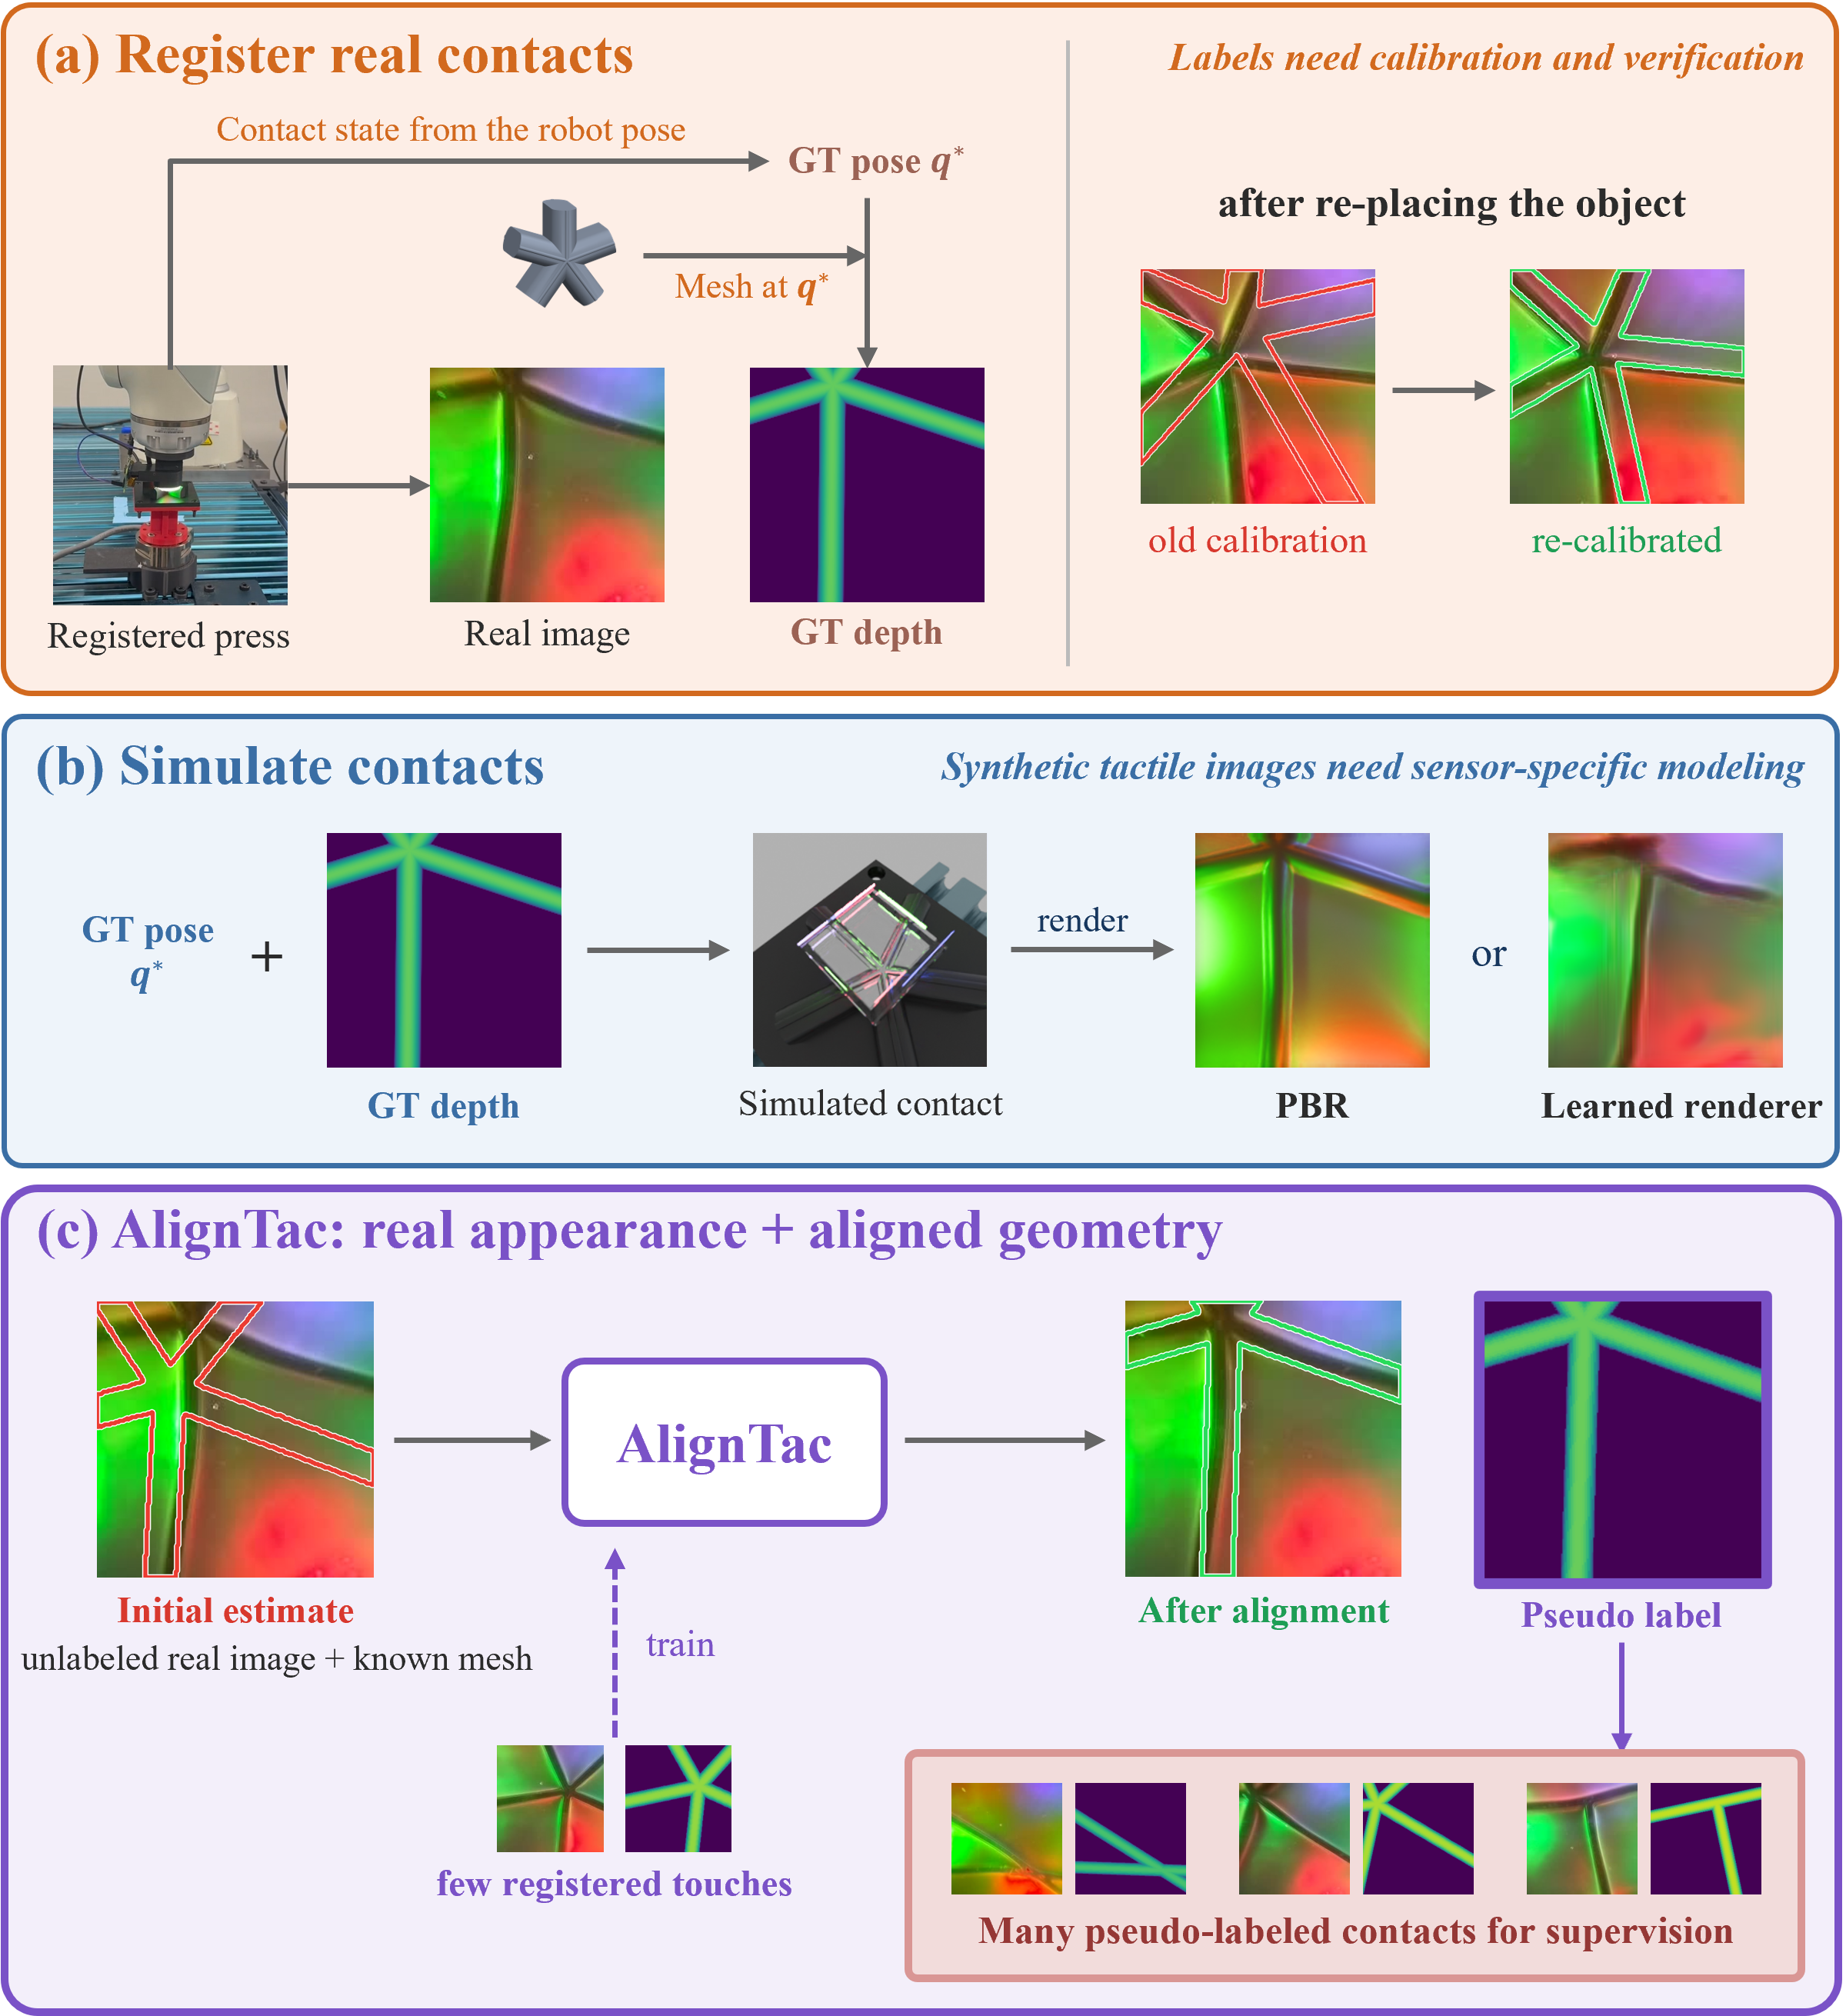
\includegraphics[width=\columnwidth]{figures/intro_figure/AlignTac_Fig1.png}
    \caption{\textbf{From registered labels to aligned geometric supervision.}
    (a) A real contact is labeled by projecting the object mesh at the contact state $q^\ast$ obtained from the robot pose; this needs calibration and verification, repeated after the object is re-placed (right; outlines mark the mesh contact region).
    (b) In simulation the state and depth are given, but tactile images need sensor-specific modeling: a physically based renderer (PBR) or a learned renderer fitted on registered real pairs.
    (c) AlignTac learns from a few registered contacts to align the known mesh with an unlabeled real image, turning the initial estimate into a pseudo-label; the bottom row shows pseudo-labeled contacts of other objects.}
    \label{fig:aligntac_teaser}
\end{figure}

Tactile perception provides robots with contact feedback for dexterous manipulation and physical interaction. Vision-based tactile sensors such as GelSight, GelSlim and DIGIT~\cite{yuan2017gelsight,donlon2018gelslim,lambeta2020digit} use a soft elastomer membrane to convert fine contact-induced deformations into high-resolution visual signals. Learning to recover contact geometry and pose supports perception through touch, but requires scalable, accurately labeled data. A known object mesh can supply these labels only after its contact state is registered to the image.

As shown in Fig.~\ref{fig:aligntac_teaser}a, real data collection requires each labeled contact to be registered. Submillimeter image--geometry accuracy depends on calibration across the robot, sensor and object frames. Systematic kinematic errors can bias the estimated contact state, including on Franka manipulators~\cite{franzese2025mukca}, while sensor mounting and object placement introduce additional uncertainty. A recorded robot pose thus becomes a label only after calibration and verification, repeated whenever the sensor configuration or object placement changes: tactile images are easier to collect than registered labels.

\begin{figure*}[t]
    \centering
    \resizebox{\textwidth}{!}{% Generated from pipeline_layout.pptx; edit this TikZ source or the exporter label definitions.
% Uses the exact notation definitions and math font of the main manuscript.
\definecolor{pc0}{HTML}{FFEFE4}%
\definecolor{pc1}{HTML}{E58844}%
\definecolor{pc2}{HTML}{20252B}%
\definecolor{pc3}{HTML}{F5F1FB}%
\definecolor{pc4}{HTML}{7550AA}%
\definecolor{pc5}{HTML}{FFFFFF}%
\definecolor{pc6}{HTML}{D3D8DE}%
\definecolor{pc7}{HTML}{626B75}%
\definecolor{pc8}{HTML}{606872}%
\definecolor{pc9}{HTML}{CEBBE4}%
\definecolor{pc10}{HTML}{FFF7F1}%
\definecolor{pc11}{HTML}{F0BE96}%
\definecolor{pc12}{HTML}{626B78}%
\definecolor{pc13}{HTML}{DF5C12}%
\definecolor{pc14}{HTML}{FAFAFC}%
\definecolor{pc15}{HTML}{CFD4DE}%
\definecolor{pc16}{HTML}{ADB3BD}%
\definecolor{pc17}{HTML}{CABBDF}%
\definecolor{pc18}{HTML}{23272F}%
\definecolor{pc19}{HTML}{F4C4A4}%
\begin{tikzpicture}[x=1bp,y=-1bp]
\path[use as bounding box] (0,0) rectangle (1152.0000,635.0400);
\begin{scope}
% Aligned pseudo-labels / full-height generation panel
\path[fill=pc0,draw=pc1,line width=0.8500bp,rounded corners=8.770bp] (874.8000,59.0400) rectangle (1125.3600,362.8800);
% Panel a heading
\node[anchor=west,inner sep=0pt,text=pc2,font=\fontsize{26.00bp}{29.12bp}\selectfont] at (25.2000,28.0800) {\textbf{(a) Training}};
% Image–geometry alignment panel
\path[fill=pc3,draw=none,rounded corners=9.115bp] (308.8800,59.0400) rectangle (827.2800,362.8800);
% Alignment panel title
\node[anchor=west,inner sep=0pt,text=pc4,font=\fontsize{24.00bp}{26.88bp}\selectfont] at (329.0400,80.6400) {\textbf{Image--geometry alignment}};
% Unlabeled collection label
\node[anchor=center,inner sep=0pt,text=pc2,font=\fontsize{21.00bp}{23.52bp}\selectfont] at (87.4800,234.3600) {\textbf{Unlabeled}};
% Unlabeled real tactile image collection: rear card 2
\path[fill=pc5,draw=pc6,line width=0.6500bp] (36.0000,247.6800) rectangle (102.9600,314.6400);
% Unlabeled real tactile image collection: rear card 1
\path[fill=pc5,draw=pc6,line width=0.6500bp] (41.0400,252.0000) rectangle (108.0000,318.9600);
% Unlabeled real tactile image collection
\node[anchor=north west,inner sep=0pt] at (46.0800,256.3200) {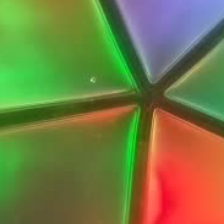
\includegraphics[width=66.9600bp,height=66.9600bp]{figures/pipeline_assets/asset_01.png}};
% Known input identity
\node[anchor=center,inner sep=0pt,text=pc7,font=\fontsize{20.00bp}{22.40bp}\selectfont] at (79.5600,337.3200) {$\Tactile,\,o$};
% Teacher module
\path[fill=pc5,draw=pc6,line width=0.8500bp,rounded corners=2.560bp] (151.2000,258.4800) rectangle (267.8400,315.3600);
% Unlabeled image to teacher
\draw[draw=pc8,line width=0.8500bp,line cap=round,-{Triangle[length=3.4bp,width=3bp]}] (118.0800,287.2800) -- (150.4799,287.2800);
% Teacher state to mesh projection
\draw[draw=pc8,line width=0.8500bp,line cap=round,-{Triangle[length=3.4bp,width=3bp]}] (268.5600,287.2800) -- (331.2000,287.2800);
% Initial state symbol
\node[anchor=center,inner sep=0pt,text=pc7,font=\fontsize{21.00bp}{23.52bp}\selectfont] at (298.8000,266.7600) {$q_0$};
% Object mesh
\node[anchor=north west,inner sep=0pt] at (337.6800,222.4800) {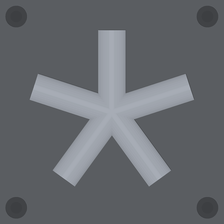
\includegraphics[width=27.3600bp,height=27.3600bp]{figures/pipeline_assets/asset_02.png}};
% Object mesh caption
\node[anchor=west,inner sep=0pt,text=pc7,font=\fontsize{19.00bp}{21.28bp}\selectfont] at (370.8000,235.4400) {Object mesh};
% Mesh input to projection
\draw[draw=pc8,line width=0.8000bp,line cap=round,-{Triangle[length=3.4bp,width=3bp]}] (351.3600,251.2799) -- (351.3600,257.7600);
% Real tactile image input to aligner
\node[anchor=north west,inner sep=0pt] at (596.1599,222.4800) {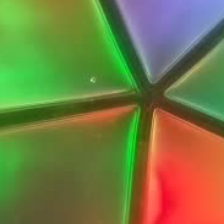
\includegraphics[width=27.3600bp,height=27.3600bp]{figures/pipeline_assets/asset_01.png}};
% Real tactile image caption
\node[anchor=west,inner sep=0pt,text=pc7,font=\fontsize{20.00bp}{22.40bp}\selectfont] at (631.4400,235.4400) {$\Tactile$};
% Real image input to aligner
\draw[draw=pc8,line width=0.8000bp,line cap=round,-{Triangle[length=3.4bp,width=3bp]}] (609.8400,251.2800) -- (609.8400,257.7600);
% Mesh projection module
\path[fill=pc5,draw=pc9,line width=0.8500bp,rounded corners=1.706bp] (331.9200,258.4800) rectangle (457.2000,315.3600);
% Projection label
\node[anchor=center,inner sep=0pt,text=pc2,font=\fontsize{21.00bp}{23.52bp}\selectfont] at (394.5600,275.0400) {\textbf{Projection}};
% Projection map
\node[anchor=center,inner sep=0pt,text=pc7,font=\fontsize{20.00bp}{22.40bp}\selectfont] at (394.5600,301.3200) {$d(\Mesh,q_t)$};
% Residual aligner module
\path[fill=pc5,draw=pc4,line width=1.2000bp,rounded corners=1.706bp] (505.4400,258.4800) rectangle (636.4800,315.3600);
% Residual aligner label
\node[anchor=center,inner sep=0pt,text=pc4,font=\fontsize{22.00bp}{24.64bp}\selectfont] at (570.9600,286.2000) {\textbf{Aligner}~$\Aligner$};
% State update module
\path[fill=pc5,draw=pc9,line width=0.8500bp,rounded corners=1.706bp] (692.6400,258.4800) rectangle (806.4000,315.3600);
% State update label
\node[anchor=center,inner sep=0pt,text=pc2,font=\fontsize{21.00bp}{23.52bp}\selectfont] at (749.5200,275.0400) {\textbf{Update}};
% Generic state update
\node[anchor=center,inner sep=0pt,text=pc7,font=\fontsize{17.50bp}{19.60bp}\selectfont] at (749.5200,300.9600) {$q_{t+1}=q_t+\Delta q$};
% Candidate projected depth to aligner
\draw[draw=pc8,line width=0.8500bp,line cap=round,-{Triangle[length=3.4bp,width=3bp]}] (457.2000,287.2800) -- (504.7200,287.2800);
% Residual correction to update
\draw[draw=pc8,line width=0.8500bp,line cap=round,-{Triangle[length=3.4bp,width=3bp]}] (637.2000,287.2800) -- (691.9200,287.2800);
% Residual symbol
\node[anchor=center,inner sep=0pt,text=pc7,font=\fontsize{20.00bp}{22.40bp}\selectfont] at (663.8400,267.8400) {$\Delta q$};
% Iterative alignment feedback / 1
\draw[draw=pc4,line width=0.8000bp,line cap=round] (749.5200,316.8000) -- (749.5200,341.2800);
% Iterative alignment feedback / 2
\draw[draw=pc4,line width=0.8000bp,line cap=round] (749.5200,341.2800) -- (394.5600,341.2800);
% Iterative alignment feedback / 3
\draw[draw=pc4,line width=0.8000bp,line cap=round,-{Triangle[length=3.4bp,width=3bp]}] (394.5600,341.2800) -- (394.5600,316.8000);
% Feedback label backing
\path[fill=pc3,draw=none] (477.3600,329.0400) rectangle (668.1600,352.0800);
% Generic iteration label
\node[anchor=center,inner sep=0pt,text=pc4,font=\fontsize{19.00bp}{21.28bp}\selectfont] at (572.7600,339.4800) {Iterative refinement};
% All real tactile images collection: rear card 2
\path[fill=pc5,draw=pc6,line width=0.6500bp] (47.5200,386.6400) rectangle (92.1600,431.2800);
% All real tactile images collection: rear card 1
\path[fill=pc5,draw=pc6,line width=0.6500bp] (52.5600,390.9600) rectangle (97.2000,435.6000);
% All real tactile images collection
\node[anchor=north west,inner sep=0pt] at (57.6000,395.2800) {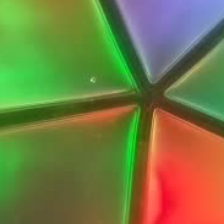
\includegraphics[width=44.6400bp,height=44.6400bp]{figures/pipeline_assets/asset_01.png}};
% All real images collection caption
\node[anchor=center,inner sep=0pt,text=pc2,font=\fontsize{20.00bp}{22.40bp}\selectfont] at (88.2000,458.6400) {All real images};
% Real training images to student
\draw[draw=pc8,line width=0.8500bp,line cap=round,-{Triangle[length=3.4bp,width=3bp]}] (108.0000,419.0400) -- (194.4000,419.0400);
% Student training module
\path[fill=pc5,draw=pc6,line width=0.8500bp,rounded corners=1.814bp] (195.8400,389.5200) rectangle (357.8400,450.0000);
% Geometric training targets panel
\path[fill=pc0,draw=pc1,line width=1.0000bp,rounded corners=2.354bp] (599.7600,386.6400) rectangle (1125.3600,465.1200);
% Registered label depth example
\node[anchor=north west,inner sep=0pt] at (646.5600,396.7200) {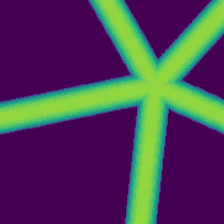
\includegraphics[width=36.0000bp,height=36.0000bp]{figures/pipeline_assets/asset_03.png}};
% Registered label normal example
\node[anchor=north west,inner sep=0pt] at (691.9200,396.7200) {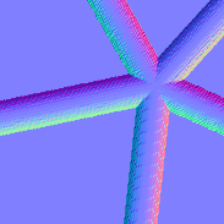
\includegraphics[width=36.0000bp,height=36.0000bp]{figures/pipeline_assets/asset_04.png}};
% Registered planar-pose target schematic / background
\path[fill=pc10,draw=pc11,line width=0.8000bp,rounded corners=0.900bp] (737.2800,396.7200) rectangle (773.2800,432.7200);
% Registered planar-pose target schematic / x axis
\draw[draw=pc12,line width=1.0000bp,line cap=round,-{Triangle[length=3.4bp,width=3bp]}] (745.9200,424.4400) -- (767.1600,424.4400);
% Registered planar-pose target schematic / y axis
\draw[draw=pc12,line width=1.0000bp,line cap=round,-{Triangle[length=3.4bp,width=3bp]}] (745.9200,424.4400) -- (745.9200,402.4800);
% Registered planar-pose target schematic / pose frame 0
\draw[draw=pc13,line width=1.0000bp,line cap=round] (748.4174,414.4587) -- (762.6121,405.9297);
% Registered planar-pose target schematic / pose frame 1
\draw[draw=pc13,line width=1.0000bp,line cap=round] (762.6121,405.9297) -- (765.0225,409.9412);
% Registered planar-pose target schematic / pose frame 2
\draw[draw=pc13,line width=1.0000bp,line cap=round] (765.0225,409.9412) -- (750.8278,418.4702);
% Registered planar-pose target schematic / pose frame 3
\draw[draw=pc13,line width=1.0000bp,line cap=round] (750.8278,418.4702) -- (748.4174,414.4587);
% Registered planar-pose target schematic / origin
\path[fill=pc13,draw=pc13,line width=1.0000bp] (745.9199,424.4399) ellipse [x radius=0.9720bp,y radius=0.9720bp];
% Registered targets caption
\node[anchor=center,inner sep=0pt,text=pc13,font=\fontsize{20.00bp}{22.40bp}\selectfont] at (709.9200,451.4400) {GT labels};
% Targets plus
\node[anchor=center,inner sep=0pt,text=pc13,font=\fontsize{24.00bp}{26.88bp}\selectfont] at (846.0000,416.1600) {+};
% Aligned label depth example
\node[anchor=north west,inner sep=0pt] at (924.4800,396.7200) {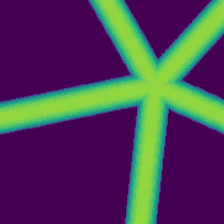
\includegraphics[width=36.0000bp,height=36.0000bp]{figures/pipeline_assets/asset_03.png}};
% Aligned label normal example
\node[anchor=north west,inner sep=0pt] at (969.8400,396.7200) {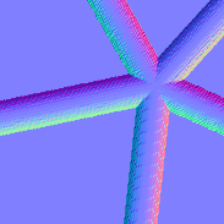
\includegraphics[width=36.0000bp,height=36.0000bp]{figures/pipeline_assets/asset_04.png}};
% Aligned planar-pose target schematic / background
\path[fill=pc10,draw=pc11,line width=0.8000bp,rounded corners=0.900bp] (1015.2000,396.7200) rectangle (1051.2000,432.7200);
% Aligned planar-pose target schematic / x axis
\draw[draw=pc12,line width=1.0000bp,line cap=round,-{Triangle[length=3.4bp,width=3bp]}] (1023.8399,424.4400) -- (1045.0799,424.4400);
% Aligned planar-pose target schematic / y axis
\draw[draw=pc12,line width=1.0000bp,line cap=round,-{Triangle[length=3.4bp,width=3bp]}] (1023.8399,424.4400) -- (1023.8399,402.4800);
% Aligned planar-pose target schematic / pose frame 0
\draw[draw=pc13,line width=1.0000bp,line cap=round] (1026.3374,414.4587) -- (1040.5321,405.9297);
% Aligned planar-pose target schematic / pose frame 1
\draw[draw=pc13,line width=1.0000bp,line cap=round] (1040.5321,405.9297) -- (1042.9425,409.9412);
% Aligned planar-pose target schematic / pose frame 2
\draw[draw=pc13,line width=1.0000bp,line cap=round] (1042.9425,409.9412) -- (1028.7478,418.4702);
% Aligned planar-pose target schematic / pose frame 3
\draw[draw=pc13,line width=1.0000bp,line cap=round] (1028.7478,418.4702) -- (1026.3374,414.4587);
% Aligned planar-pose target schematic / origin
\path[fill=pc13,draw=pc13,line width=1.0000bp] (1023.8399,424.4399) ellipse [x radius=0.9720bp,y radius=0.9720bp];
% Aligned targets caption
\node[anchor=center,inner sep=0pt,text=pc13,font=\fontsize{20.00bp}{22.40bp}\selectfont] at (987.8400,451.4400) {Pseudo-labels};
% Geometry targets supervise student
\draw[draw=pc1,line width=1.0000bp,line cap=round,dash pattern=on 3bp off 2.5bp,-{Triangle[length=3.4bp,width=3bp]}] (599.0400,419.0400) -- (359.2800,419.0400);
% Supervision arrow caption
\node[anchor=center,inner sep=0pt,text=pc13,font=\fontsize{20.00bp}{22.40bp}\selectfont] at (479.5200,402.8399) {Geometric supervision};
% Panel divider
\draw[draw=pc6,line width=0.7500bp,line cap=round] (25.2000,483.8400) -- (1125.3600,483.8400);
% Panel b heading
\node[anchor=west,inner sep=0pt,text=pc2,font=\fontsize{26.00bp}{29.12bp}\selectfont] at (25.2000,508.3200) {\textbf{(b) Inference}};
% Inference real tactile image
\node[anchor=north west,inner sep=0pt] at (41.7600,547.9200) {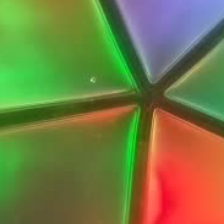
\includegraphics[width=52.5600bp,height=52.5600bp]{figures/pipeline_assets/asset_01.png}};
% Inference inputs
\node[anchor=center,inner sep=0pt,text=pc7,font=\fontsize{21.00bp}{23.52bp}\selectfont] at (122.4000,574.5600) {$\Tactile,\,o$};
% Inference input to student
\draw[draw=pc8,line width=0.8500bp,line cap=round,-{Triangle[length=3.4bp,width=3bp]}] (142.5600,574.5600) -- (174.9600,574.5600);
% Student inference module
\path[fill=pc5,draw=pc6,line width=0.8500bp,rounded corners=1.728bp] (175.6800,545.0400) rectangle (324.0000,602.6400);
% Student to predicted geometry
\draw[draw=pc8,line width=0.8500bp,line cap=round,-{Triangle[length=3.4bp,width=3bp]}] (324.7200,574.5600) -- (362.8800,574.5600);
% Predicted depth illustration
\node[anchor=north west,inner sep=0pt] at (368.6400,546.4800) {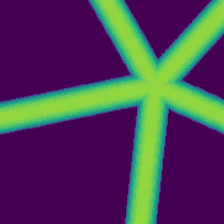
\includegraphics[width=48.9600bp,height=48.9600bp]{figures/pipeline_assets/asset_03.png}};
% Predicted normals illustration
\node[anchor=north west,inner sep=0pt] at (443.5200,546.4800) {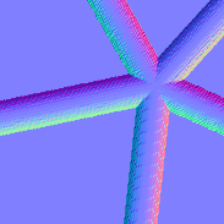
\includegraphics[width=48.9600bp,height=48.9600bp]{figures/pipeline_assets/asset_04.png}};
% Predicted planar pose schematic / x axis
\draw[draw=pc12,line width=0.7500bp,line cap=round,-{Triangle[length=3.4bp,width=3bp]}] (529.4304,584.1791) -- (558.3168,584.1791);
% Predicted planar pose schematic / y axis
\draw[draw=pc12,line width=0.7500bp,line cap=round,-{Triangle[length=3.4bp,width=3bp]}] (529.4304,584.1791) -- (529.4304,554.3135);
% Predicted planar pose schematic / pose frame 0
\draw[draw=pc13,line width=1.1000bp,line cap=round] (532.8269,570.6046) -- (552.1317,559.0052);
% Predicted planar pose schematic / pose frame 1
\draw[draw=pc13,line width=1.1000bp,line cap=round] (552.1317,559.0052) -- (555.4098,564.4609);
% Predicted planar pose schematic / pose frame 2
\draw[draw=pc13,line width=1.1000bp,line cap=round] (555.4098,564.4609) -- (536.1050,576.0603);
% Predicted planar pose schematic / pose frame 3
\draw[draw=pc13,line width=1.1000bp,line cap=round] (536.1050,576.0603) -- (532.8269,570.6046);
% Predicted planar pose schematic / origin
\path[fill=pc13,draw=pc13,line width=1.0000bp] (529.4303,584.1791) ellipse [x radius=1.3219bp,y radius=1.3219bp];
% Inference depth caption
\node[anchor=center,inner sep=0pt,text=pc2,font=\fontsize{20.00bp}{22.40bp}\selectfont] at (393.1200,608.0400) {Depth};
% Inference normals caption
\node[anchor=center,inner sep=0pt,text=pc2,font=\fontsize{20.00bp}{22.40bp}\selectfont] at (468.7200,608.0400) {Normals};
% Inference pose caption
\node[anchor=center,inner sep=0pt,text=pc2,font=\fontsize{20.00bp}{22.40bp}\selectfont] at (542.1600,608.0400) {Pose};
% Optional pose refinement boundary
\path[fill=pc14,draw=pc15,line width=0.7500bp,dash pattern=on 3bp off 2.5bp,rounded corners=2.163bp] (628.5600,501.1200) rectangle (1125.3600,621.3600);
% Optional branch heading
\node[anchor=center,inner sep=0pt,text=pc12,font=\fontsize{20.00bp}{22.40bp}\selectfont] at (876.2400,516.9600) {Pose refinement (optional)};
% Optional branch initial state
\node[anchor=center,inner sep=0pt,text=pc7,font=\fontsize{20.00bp}{22.40bp}\selectfont] at (665.2800,556.5600) {$q_0$};
% Optional refinement real image
\node[anchor=north west,inner sep=0pt] at (797.7600,534.2400) {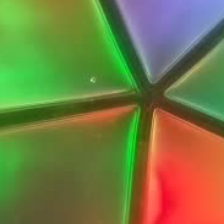
\includegraphics[width=18.0000bp,height=18.0000bp]{figures/pipeline_assets/asset_01.png}};
% Optional refinement object mesh
\node[anchor=north west,inner sep=0pt] at (825.1200,534.2400) {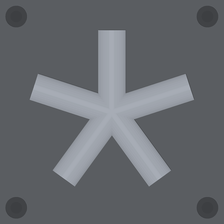
\includegraphics[width=18.0000bp,height=18.0000bp]{figures/pipeline_assets/asset_02.png}};
% Reused residual aligner module
\path[fill=pc5,draw=pc9,line width=0.8500bp,rounded corners=1.498bp] (764.6400,555.8400) rectangle (891.3600,593.2800);
% Optional aligner name
\node[anchor=center,inner sep=0pt,text=pc4,font=\fontsize{22.00bp}{24.64bp}\selectfont] at (828.0000,573.8400) {\textbf{Aligner}~$\Aligner$};
% Refined planar pose schematic / x axis
\draw[draw=pc12,line width=1.0000bp,line cap=round,-{Triangle[length=3.4bp,width=3bp]}] (960.7104,584.1791) -- (989.5968,584.1791);
% Refined planar pose schematic / y axis
\draw[draw=pc12,line width=1.0000bp,line cap=round,-{Triangle[length=3.4bp,width=3bp]}] (960.7104,584.1791) -- (960.7104,554.3135);
% Refined planar pose schematic / pose frame 0
\draw[draw=pc13,line width=1.0000bp,line cap=round] (964.1069,570.6046) -- (983.4117,559.0052);
% Refined planar pose schematic / pose frame 1
\draw[draw=pc13,line width=1.0000bp,line cap=round] (983.4117,559.0052) -- (986.6898,564.4609);
% Refined planar pose schematic / pose frame 2
\draw[draw=pc13,line width=1.0000bp,line cap=round] (986.6898,564.4609) -- (967.3850,576.0603);
% Refined planar pose schematic / pose frame 3
\draw[draw=pc13,line width=1.0000bp,line cap=round] (967.3850,576.0603) -- (964.1069,570.6046);
% Refined planar pose schematic / origin
\path[fill=pc13,draw=pc13,line width=1.0000bp] (960.7103,584.1791) ellipse [x radius=1.3219bp,y radius=1.3219bp];
% Refined output caption
\node[anchor=center,inner sep=0pt,text=pc2,font=\fontsize{20.00bp}{22.40bp}\selectfont] at (1064.1600,574.5600) {Refined pose};
% Registered contacts heading
\node[anchor=west,inner sep=0pt,text=pc2,font=\fontsize{23.00bp}{25.76bp}\selectfont] at (25.2000,84.2400) {\textbf{Labeled contacts}};
% Registered tactile observation I
\node[anchor=north west,inner sep=0pt] at (40.3200,108.7200) {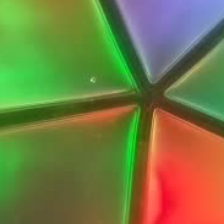
\includegraphics[width=40.3200bp,height=40.3200bp]{figures/pipeline_assets/asset_01.png}};
% Registered object mesh M
\node[anchor=north west,inner sep=0pt] at (102.9600,108.7200) {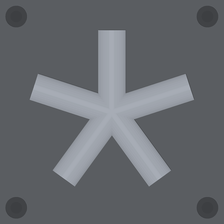
\includegraphics[width=40.3200bp,height=40.3200bp]{figures/pipeline_assets/asset_02.png}};
% Registered input I
\node[anchor=center,inner sep=0pt,text=pc7,font=\fontsize{20.00bp}{22.40bp}\selectfont] at (60.4800,163.8000) {$\Tactile$};
% Registered input M
\node[anchor=center,inner sep=0pt,text=pc7,font=\fontsize{20.00bp}{22.40bp}\selectfont] at (123.1200,163.8000) {$\Mesh$};
% Registered state x axis
\draw[draw=pc7,line width=0.6500bp,line cap=round,-{Triangle[length=3.4bp,width=3bp]}] (171.3600,145.4400) -- (230.4000,145.4400);
% Registered state y axis
\draw[draw=pc7,line width=0.6500bp,line cap=round,-{Triangle[length=3.4bp,width=3bp]}] (171.3600,145.4400) -- (171.3600,105.8400);
% Registered state schematic edge 1
\draw[draw=pc7,line width=1.1000bp,line cap=round] (181.1593,131.6587) -- (218.9428,110.7149);
% Registered state schematic edge 2
\draw[draw=pc7,line width=1.1000bp,line cap=round] (218.9428,110.7149) -- (223.4806,118.9013);
% Registered state schematic edge 3
\draw[draw=pc7,line width=1.1000bp,line cap=round] (223.4806,118.9013) -- (185.6971,139.8450);
% Registered state schematic edge 4
\draw[draw=pc7,line width=1.1000bp,line cap=round] (185.6971,139.8450) -- (181.1593,131.6587);
% Registered state q star
\node[anchor=center,inner sep=0pt,text=pc7,font=\fontsize{20.00bp}{22.40bp}\selectfont] at (200.1600,163.8000) {$q^\ast$};
% Registered state and mesh to perturbation
\draw[draw=pc7,line width=0.9500bp,line cap=round,-{Triangle[length=3.4bp,width=3bp]}] (247.6800,134.6400) -- (328.3199,134.6400);
% Registered supervision trains teacher
\draw[draw=pc7,line width=0.9500bp,line cap=round,dash pattern=on 3bp off 2.5bp,-{Triangle[length=3.4bp,width=3bp]}] (209.5200,181.4400) -- (209.5200,257.0400);
% Teacher training connection
\node[anchor=west,inner sep=0pt,text=pc7,font=\fontsize{18.00bp}{20.16bp}\selectfont] at (217.4400,217.4400) {train};
% Perturb and project stage
\node[anchor=center,inner sep=0pt,text=pc4,font=\fontsize{19.00bp}{21.28bp}\selectfont] at (395.2799,108.3600) {\textbf{Perturb + project}};
% Original registered state ghost edge 1
\draw[draw=pc16,line width=1.0000bp,line cap=round,dash pattern=on 3bp off 2.5bp] (347.0066,145.2656) -- (401.0430,124.5788);
% Original registered state ghost edge 2
\draw[draw=pc16,line width=1.0000bp,line cap=round,dash pattern=on 3bp off 2.5bp] (401.0430,124.5788) -- (406.1133,131.4446);
% Original registered state ghost edge 3
\draw[draw=pc16,line width=1.0000bp,line cap=round,dash pattern=on 3bp off 2.5bp] (406.1133,131.4446) -- (352.0769,152.1314);
% Original registered state ghost edge 4
\draw[draw=pc16,line width=1.0000bp,line cap=round,dash pattern=on 3bp off 2.5bp] (352.0769,152.1313) -- (347.0066,145.2656);
% Perturbed candidate state edge 1
\draw[draw=pc4,line width=1.4500bp,line cap=round] (363.5062,130.8320) -- (424.1106,124.6994);
% Perturbed candidate state edge 2
\draw[draw=pc4,line width=1.4500bp,line cap=round] (424.1106,124.6994) -- (425.6137,132.3998);
% Perturbed candidate state edge 3
\draw[draw=pc4,line width=1.4500bp,line cap=round] (425.6137,132.3998) -- (365.0093,138.5324);
% Perturbed candidate state edge 4
\draw[draw=pc4,line width=1.4500bp,line cap=round] (365.0093,138.5324) -- (363.5062,130.8320);
% Geometric displacement delta
\draw[draw=pc4,line width=1.0000bp,line cap=round,-{Triangle[length=3.4bp,width=3bp]}] (364.3200,146.6495) -- (391.6800,140.9471);
% State perturbation delta
\node[anchor=west,inner sep=0pt,text=pc4,font=\fontsize{19.00bp}{21.28bp}\selectfont] at (403.2000,148.7231) {$\delta$};
% Projected perturbed depth
\node[anchor=center,inner sep=0pt,text=pc7,font=\fontsize{19.00bp}{21.28bp}\selectfont] at (395.2800,173.8800) {$d(\Mesh,q^\ast+\delta)$};
% Aligner training module
\path[fill=pc5,draw=pc4,line width=1.2000bp,rounded corners=1.764bp] (505.4400,149.0399) rectangle (636.4800,199.4399);
% Aligner training module label
\node[anchor=center,inner sep=0pt,text=pc4,font=\fontsize{22.00bp}{24.64bp}\selectfont] at (570.9600,173.8799) {\textbf{Aligner}~$\Aligner$};
% Real tactile observation for aligner training
\node[anchor=north west,inner sep=0pt] at (551.5200,102.9600) {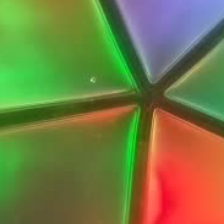
\includegraphics[width=28.0800bp,height=28.0800bp]{figures/pipeline_assets/asset_01.png}};
% Real tactile training input symbol
\node[anchor=west,inner sep=0pt,text=pc7,font=\fontsize{20.00bp}{22.40bp}\selectfont] at (586.0800,115.9200) {$\Tactile$};
% Known corrective target label
\node[anchor=center,inner sep=0pt,text=pc4,font=\fontsize{18.00bp}{20.16bp}\selectfont] at (748.0800,116.6400) {Correction target};
% Correction learning target
\path[fill=pc5,draw=pc17,line width=0.9000bp,rounded corners=1.764bp] (692.6400,149.0399) rectangle (806.4000,199.4399);
% Corrective supervision delta
\node[anchor=center,inner sep=0pt,text=pc4,font=\fontsize{22.00bp}{24.64bp}\selectfont] at (749.5200,173.8799) {$\Delta q\approx-\delta$};
% Weight reuse label
\node[anchor=west,inner sep=0pt,text=pc4,font=\fontsize{17.50bp}{19.60bp}\selectfont] at (534.2400,219.2400) {\textit{reuse}~$\Aligner$};
% Perturbed state projected to depth
\draw[draw=pc4,line width=0.9000bp,line cap=round,-{Triangle[length=3.4bp,width=3bp]}] (393.1200,151.2000) -- (393.1200,159.1200);
% Perturbed depth enters training aligner
\draw[draw=pc4,line width=1.0000bp,line cap=round,-{Triangle[length=3.4bp,width=3bp]}] (465.8400,174.2400) -- (504.0000,174.2400);
% Aligner predicts residual for known corrective target
\draw[draw=pc4,line width=1.0000bp,line cap=round,-{Triangle[length=3.4bp,width=3bp]}] (637.9199,174.2400) -- (691.2000,174.2400);
% Real image enters training aligner
\draw[draw=pc12,line width=0.9000bp,line cap=round,-{Triangle[length=3.4bp,width=3bp]}] (565.5600,133.2000) -- (565.5600,147.5999);
% Reuse learned aligner weights
\draw[draw=pc4,line width=0.9500bp,line cap=round,dash pattern=on 3bp off 2.5bp,-{Triangle[length=3.4bp,width=3bp]}] (525.6000,200.8800) -- (525.6000,257.0400);
% Image and mesh to optional aligner
\draw[draw=pc12,line width=0.9000bp,line cap=round,-{Triangle[length=3.4bp,width=3bp]}] (820.8000,552.6000) -- (820.8000,555.1200);
% Horizontal initialization arrow
\draw[draw=pc12,line width=1.1000bp,line cap=round,-{Triangle[length=3.4bp,width=3bp]}] (580.3200,574.5600) -- (763.2000,574.5600);
% Optional aligner to refined pose
\draw[draw=pc12,line width=1.0000bp,line cap=round,-{Triangle[length=3.4bp,width=3bp]}] (892.8000,574.5600) -- (943.2000,574.5600);
% Teacher / role label (Teacher module)
% Teacher / mathematical model (Teacher module)
\node[anchor=center,inner sep=0pt,text=pc18,font=\fontsize{20.00bp}{22.40bp}\selectfont] at (209.5200,286.9200) {\textbf{Teacher}~$\Teacher$};
% Student / role label (Student training module)
% Student / mathematical model (Student training module)
\node[anchor=center,inner sep=0pt,text=pc18,font=\fontsize{20.00bp}{22.40bp}\selectfont] at (276.8400,419.7600) {\textbf{Student}~$\Student$};
% Student / role label (Student inference module)
% Student / mathematical model (Student inference module)
\node[anchor=center,inner sep=0pt,text=pc18,font=\fontsize{20.00bp}{22.40bp}\selectfont] at (249.8400,573.8400) {\textbf{Student}~$\Student$};
% Aligned pseudo-labels / heading
\node[anchor=center,inner sep=0pt,text=pc13,font=\fontsize{23.00bp}{25.76bp}\selectfont] at (1000.0800,82.0800) {\textbf{Aligned pseudo-labels}};
% Known mesh for geometric targets
\node[anchor=north west,inner sep=0pt] at (936.0000,111.6000) {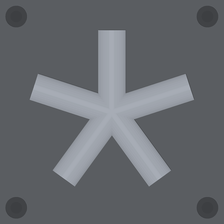
\includegraphics[width=34.5600bp,height=34.5600bp]{figures/pipeline_assets/asset_02.png}};
% Known mesh for targets / label
\node[anchor=west,inner sep=0pt,text=pc7,font=\fontsize{20.00bp}{22.40bp}\selectfont] at (978.4800,126.3600) {Mesh~$\Mesh$};
% Known mesh enters target generator
\draw[draw=pc13,line width=0.9000bp,line cap=round,-{Triangle[length=3.4bp,width=3bp]}] (1000.0800,149.7600) -- (1000.0800,162.7199);
% Geometric target generator
\path[fill=pc5,draw=pc19,line width=0.8000bp,rounded corners=1.814bp] (903.6000,165.6000) rectangle (1098.0000,226.0800);
% Geometric target generator / name
\node[anchor=center,inner sep=0pt,text=pc2,font=\fontsize{21.00bp}{23.52bp}\selectfont] at (1000.8000,182.8800) {\textbf{Geometric targets}};
% Geometric target generator / map
\node[anchor=center,inner sep=0pt,text=pc13,font=\fontsize{20.00bp}{22.40bp}\selectfont] at (1000.8000,209.8800) {$\Targets(\Mesh,q_T)$};
% Aligned state into target generator / outlet
\draw[draw=pc7,line width=0.9000bp,line cap=round] (806.4000,287.2800) -- (850.3200,287.2800);
% Aligned state into target generator / rise
\draw[draw=pc7,line width=0.9000bp,line cap=round] (850.3200,287.2800) -- (850.3200,195.8400);
% Aligned state into target generator / input
\draw[draw=pc7,line width=0.9000bp,line cap=round,-{Triangle[length=3.4bp,width=3bp]}] (850.3200,195.8400) -- (902.1600,195.8400);
% Aligned state q_T
\node[anchor=center,inner sep=0pt,text=pc7,font=\fontsize{21.00bp}{23.52bp}\selectfont] at (837.7200,268.5600) {$q_T$};
% Geometric target generator to outputs
\draw[draw=pc13,line width=0.9000bp,line cap=round,-{Triangle[length=3.4bp,width=3bp]}] (1000.0800,227.5200) -- (1000.0800,249.1200);
% Depth pseudo-label: original projected geometry
\node[anchor=north west,inner sep=0pt] at (891.3600,258.4800) {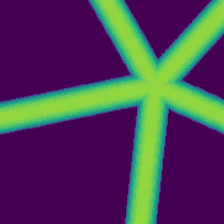
\includegraphics[width=58.3200bp,height=58.3200bp]{figures/pipeline_assets/asset_03.png}};
% Normal pseudo-label: original projected geometry
\node[anchor=north west,inner sep=0pt] at (969.8400,258.4800) {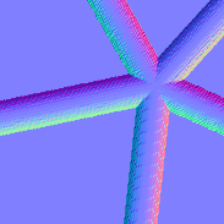
\includegraphics[width=58.3200bp,height=58.3200bp]{figures/pipeline_assets/asset_04.png}};
% Planar-pose pseudo-label schematic / background
\path[fill=pc10,draw=pc11,line width=0.8000bp,rounded corners=1.458bp] (1049.0400,258.4800) rectangle (1107.3600,316.8000);
% Planar-pose pseudo-label schematic / x axis
\draw[draw=pc12,line width=1.0000bp,line cap=round,-{Triangle[length=3.4bp,width=3bp]}] (1063.0368,303.3863) -- (1097.4455,303.3863);
% Planar-pose pseudo-label schematic / y axis
\draw[draw=pc12,line width=1.0000bp,line cap=round,-{Triangle[length=3.4bp,width=3bp]}] (1063.0368,303.3863) -- (1063.0368,267.8111);
% Planar-pose pseudo-label schematic / pose frame 0
\draw[draw=pc13,line width=1.0000bp,line cap=round] (1067.0826,287.2167) -- (1090.0780,273.3997);
% Planar-pose pseudo-label schematic / pose frame 1
\draw[draw=pc13,line width=1.0000bp,line cap=round] (1090.0780,273.3997) -- (1093.9828,279.8983);
% Planar-pose pseudo-label schematic / pose frame 2
\draw[draw=pc13,line width=1.0000bp,line cap=round] (1093.9828,279.8983) -- (1070.9874,293.7154);
% Planar-pose pseudo-label schematic / pose frame 3
\draw[draw=pc13,line width=1.0000bp,line cap=round] (1070.9874,293.7154) -- (1067.0826,287.2167);
% Planar-pose pseudo-label schematic / origin
\path[fill=pc13,draw=pc13,line width=1.0000bp] (1063.0368,303.3864) ellipse [x radius=1.5746bp,y radius=1.5746bp];
% Geometric output / Depth
\node[anchor=center,inner sep=0pt,text=pc2,font=\fontsize{21.00bp}{23.52bp}\selectfont] at (921.6000,335.1600) {Depth};
% Geometric output / Normals
\node[anchor=center,inner sep=0pt,text=pc2,font=\fontsize{21.00bp}{23.52bp}\selectfont] at (1000.0800,335.1600) {Normals};
% Geometric output / Pose
\node[anchor=center,inner sep=0pt,text=pc2,font=\fontsize{21.00bp}{23.52bp}\selectfont] at (1080.0000,335.1600) {Pose};
% Pseudo-labels enter student supervision
\draw[draw=pc13,line width=0.9000bp,line cap=round,dash pattern=on 3bp off 2.5bp,-{Triangle[length=3.4bp,width=3bp]}] (1000.0800,364.3200) -- (1000.0800,385.2000);
\end{scope}
\end{tikzpicture}%
}
    \caption{\textbf{AlignTac training and inference.} (a) Registered contacts train teacher $\Teacher$ and aligner $\Aligner$. The upper branch trains $\Aligner$ from the real image and mesh depth at $q^\ast+\delta$, using correction target $-\delta$. The lower branch refines teacher-initialized states of unlabeled contacts. The aligned state $q_T$ and mesh $\Mesh$ yield depth, normal and planar-pose targets through $\Targets(\Mesh,q_T)$. Student $\Student$ learns from registered and pseudo-labeled real images. (b) Standard prediction uses the image and object identity; mesh-assisted pose refinement is \FinalLine{optional. Thumbnails show a real contact; pose and perturbation glyphs are schematic.}}
    \label{fig:mapl}
\end{figure*}

Simulation and self-training offer two ways to use a small labeled set. Simulation provides geometric targets from known meshes~\cite{wang2022tacto,si2022taxim,chen2023tacchi} (see Fig.~\ref{fig:aligntac_teaser}b), while a renderer must reproduce tactile appearance: illumination, surface reflectance and contact-induced deformation jointly determine the image~\cite{si2022taxim,agarwal2021simulation}. Sensor-specific calibration or fitting on real image--geometry pairs adapts the renderer's appearance; the labeled pairs used for fitting also consume the registration budget. Self-training instead uses a predictor's outputs to label remaining real images and can propagate its errors~\cite{arazo2020pseudo}.

As illustrated in Fig.~\ref{fig:aligntac_teaser}c, our AlignTac combines real tactile appearance with known simulated geometry through contact-state alignment. For a known object, its mesh specifies the geometry, but dense labels depend on a low-dimensional contact state: in-plane rotation, translation and indentation. Obtaining this state for an unlabeled image is difficult: thin contact features make dense labels sensitive to small state errors, mesh depth cannot be compared with tactile RGB directly, and only the few registered contacts are available to learn the correspondence. AlignTac therefore learns the contact-state correction that aligns mesh projections with real tactile observations.

AlignTac learns this alignment from a small registered set (Fig.~\ref{fig:mapl}). We perturb each contact's mesh state while keeping its real image fixed, and train a residual aligner to recover the registered state. For additional real contacts, teacher $\Teacher$ provides the initial state, the aligner corrects it using the observed image, and the aligned geometry supplies depth, normal and planar-pose pseudo-labels. A student $\Student$ learns from these labels and predicts directly from \FinalLine{the tactile image and object identity.}

We evaluate AlignTac against self-training and synthetic augmentation on two GelSlim~4.0 variants: marker-free (sensor A) and dot-marker (sensor B). Experiments use limited real-label budgets. Our contributions are:
\begin{itemize}
    \item A real-image--geometry alignment framework that learns state corrections from perturbations of a small registered set and generates dense geometry and pose \FinalLine{supervision using real tactile images.}
    \item An alignment ablation showing gains in pseudo-label quality and student accuracy, with label efficiency on both sensor variants.
    \item A second-session study in which images captured after object re-placement are labeled by the same aligner, without re-registration.
    \item A matched-budget renderer study identifying complementary benefits of tactile RGB simulation for held-out-object pose coverage and session changes, while accounting for the real labels used to fit the renderer.
\end{itemize}

\section{Related Work}

\noindent\textbf{Tactile simulation and transfer.}
TACTO~\cite{wang2022tacto}, Taxim~\cite{si2022taxim}, Tacchi~\cite{chen2023tacchi} and physics-based rendering~\cite{agarwal2021simulation} model tactile images through optical response and contact geometry or deformation. Differentiable~\cite{xu2022efficient} and GPU-based~\cite{akinola2025tacsl} simulation support learning and control. Transfer methods translate tactile appearance~\cite{chen2022cyclegan}, map real images to simulated depth~\cite{church2022tactile}, or generate tactile images from visual RGB-D~\cite{zhong2025tactgen}. Our study concerns depth-to-RGB renderers fitted on real contact pairs and counts those pairs in the training-label budget.

\noindent\textbf{Tactile geometry reconstruction.}
Prior work learns local contact shape or elastomer deformation directly from tactile images~\cite{bauza2019tactile,zhu2022volumetric}; MeshTac instead reduces the real geometric labels needed to train such predictors.

\noindent\textbf{Tactile representations.}
Pretrained encoders such as SITR, T3 and Sparsh~\cite{gupta2025sitr,zhao2024transferable,higuera2024sparsh} reduce feature learning from scratch; all our predictors share a frozen SITR backbone, and MeshTac addresses supervision rather than the encoder.

\noindent\textbf{Pseudo-labeling and pose refinement.}
Self-training uses model predictions as labels~\cite{lee2013pseudo,xie2020noisy} and can reinforce teacher errors~\cite{arazo2020pseudo}. Known geometry offers an additional constraint. DeepIM~\cite{li2018deepim} learns iterative pose corrections from observed and rendered images; Self6D~\cite{wang2020self6d} uses differentiable rendering to supervise pose on unlabeled RGB-D images. Tac2Pose~\cite{bauza2023tac2pose} estimates pose from a single touch by matching the observed contact shape to simulated contacts of a known mesh. Unlike refinement methods that improve the state estimate at inference, MeshTac learns state corrections from a few registered contacts to generate dense geometry and pose supervision for additional real images; mesh-assisted inference is optional.

\section{Mesh-Aligned Pseudo-Labeling}
\label{sec:mapl}

\begin{figure}[t]
    \centering
    \begin{tikzpicture}[font=\scriptsize, node distance=2.5mm and 3mm,
        box/.style={draw, rounded corners=1pt, align=center, inner sep=2pt, minimum height=5mm, fill=white},
        data/.style={box, fill=black!5}, model/.style={box, fill=blue!8}, rend/.style={box, fill=orange!12},
        arr/.style={-{Latex[length=1.5mm]}, thick}]
        \node[data, text width=31mm] (lab) {$\Kreal$ labeled frames per object (depth, pose)};
        \node[data, text width=26mm, right=of lab] (mesh) {object meshes};
        \node[model, text width=31mm, below=of lab] (f0) {teacher $f_0$ ($\Kreal$-shot model)};
        \node[rend, text width=26mm, below=of mesh] (al) {aligner $A$: (frame, mesh depth at pose) $\to$ pose correction};
        \node[data, text width=31mm, below=4.5mm of f0] (unl) {unlabeled frames $U$};
        \node[box, text width=26mm, right=of unl] (rc) {\textbf{align}: iterate $A$ from the teacher pose};
        \node[model, text width=31mm, below=of unl] (f1) {student $f_1$: $\Kreal$ labeled + aligned $U$};
        \node[box, text width=26mm, below=of rc] (lbl) {\textbf{label}: mesh depth, normals and pose at the aligned pose};
        \draw[arr] (lab) -- (f0); \draw[arr] (lab) -- (al); \draw[arr] (mesh) -- (al);
        \draw[arr] (f0) -- node[left, xshift=-1pt] {pose} (unl); \draw[arr] (unl) -- (rc); \draw[arr] (al) -- (rc);
        \draw[arr] (rc) -- (lbl); \draw[arr] (lbl) -- (f1);
    \end{tikzpicture}
    \caption{\textbf{Mesh-aligned pseudo-labeling.} The $\Kreal$-shot teacher proposes a pose for every unlabeled frame. An aligner trained on the same $\Kreal$ labeled frames iteratively corrects that pose until the object mesh matches the frame; the mesh at the aligned pose, not the teacher's prediction, labels the frame for the student.}
    \label{fig:mapl}
\end{figure}

\begin{figure}[t]
    \centering
    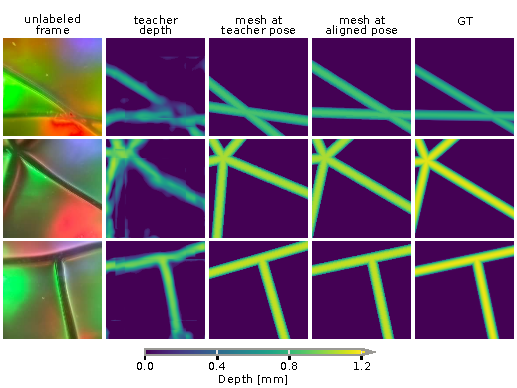
\includegraphics[width=\columnwidth]{figures/fig_align.pdf}
    \caption{\textbf{Labels of unlabeled frames} ($\Kreal=25$; each object's median-quality frame). The teacher's depth is blurred and its pose is off by several degrees; after alignment the mesh label is close to the withheld reference.}
    \label{fig:align}
\end{figure}

\noindent\textbf{Idea.} Let $d(M,q)$ be the depth map of mesh $M$ at contact state $q=(\theta,x,y,z)$ (planar pose and indentation). The reference label of a real frame $I$ of object $M$ is $d(M,q^\ast)$ for the pose $q^\ast$ at which it was captured, so labeling an unlabeled frame is a pose-estimation problem with only four unknowns, and its solution yields depth, normals and pose at once. A $\Kreal$-shot model estimates $q$ only to a few degrees and its dense output is blurred (Fig.~\ref{fig:align}); with the true pose, in contrast, the mesh label is essentially exact (contact IoU $0.95$ against the reference). MAPL closes this gap with a learned refinement.

\noindent\textbf{Residual aligner.} The aligner $A$ is a ResNet-18 (ImageNet-initialized) that takes the real frame and, as a fourth channel, the mesh depth at a candidate pose, and regresses the correction that brings the candidate onto the frame:
\begin{equation}
    A\big(I,\; d(M,q)\big) \;\approx\; q^\ast - q .
\end{equation}
It needs no label beyond the $\Kreal$ frames, because each labeled frame provides unlimited training pairs: we perturb its true pose by up to $\pm8^\circ$, $\pm1.5\,$mm in the plane and $\pm0.15\,$mm of indentation (half of the samples at $0.3\times$ that range, for fine corrections), render the mesh depth at the perturbed pose, and regress the perturbation with a smooth-L1 loss (8k steps, batch 64, AdamW, $3\times10^{-4}$). This is render-and-compare pose refinement~\cite{li2018deepim} with the mesh depth as the ``render'': no photorealistic renderer is involved.

\noindent\textbf{Labeling.} For every unlabeled training frame the teacher $f_0$ (the model trained on the $\Kreal$ labeled frames and GAN-$\Kreal$ data) predicts a pose; the indentation is initialized with the maximum of its predicted depth. The aligner is applied six times, $q\leftarrow q+A(I,d(M,q))$, and the frame receives $d(M,q)$, its normals and $q$ as labels. Every frame is used; no confidence filtering is needed (Sec.~\ref{sec:ablation}). The object of each frame is assumed known, as it is when a user collects frames object by object.

\noindent\textbf{Student.} The student $f_1$ is trained like any other model in this paper on the $\Kreal$ labeled frames, the aligned frames and synthetic frames, with full depth, normal and pose supervision. Following the $\Kreal$-shot rule, the synthetic frames come from the learned renderer retrained on the $\Kreal$ true plus the aligned (depth, image) pairs, which also makes it the most faithful leakage-free renderer of our study (contact-region image error $-13$ to $-19\%$ at every $\Kreal$); the student's accuracy, however, does not depend on this choice (Table~\ref{tab:abl}).

\noindent\textbf{Test-time alignment.} Planar pose is defined with respect to a known object, so the same aligner can also refine the pose a model predicts on a \emph{test} frame (Sec.~\ref{sec:tta}).

\noindent\textbf{Cost and scope.} MAPL adds no labels and leaves the downstream architecture unchanged; it uses the unlabeled frames and the meshes that simulation already requires. Validation and test frames are never pseudo-labeled and never seen by the aligner.

\section{Experimental Setup}
\label{sec:setup}

\noindent\textbf{Sensors and data.} Sensor A is a GelSlim-type fingertip with a $17.5\,$mm gel view and six colored LED emitters. A robot presses it against 12 ridge-pattern objects with known geometry. Ground-truth (GT) depth and normals are mesh projections at the recorded pose, rather than measurements of membrane deformation. After filtering, $4{,}669$ frames remain; every tenth frame is assigned to the validation split ($472$ frames). A second session, recorded on another day after the objects were re-placed, contains $854$ reviewed test frames from 11 objects. Their poses are re-estimated from contact masks. Sensor B, \sensorB{}~\cite{sipos2024gelslim4}, has a marker array, different illumination and a $12\,$mm view. We use its public dataset of the same 12 objects ($1{,}620$ test frames). We re-register its clipped, smoothed depth labels to the meshes by pose fitting ($0.018\,$mm mean residual) and use the resulting targets for every sensor-B method.

\noindent\textbf{Label budget.} Each object contributes $\Kreal\in\{10,25,50,100\}$ evenly spaced labeled training frames. The teacher, renderer and aligner share these frames, which represent $3\%$, $7\%$, $14\%$ and $29\%$ of the sensor-A training set. All other training images are available without labels. Our primary setting is $K\le25$; the larger budgets show how performance changes as more labels become available. Validation and test images are excluded from component training. Validation labels are used for checkpoint selection and are not included in the stated training-label budget.

\noindent\textbf{Models and training.} All methods use a frozen SITR-B/18 encoder~\cite{gupta2025sitr}, a DPT decoder~\cite{ranftl2021dpt} for depth and normals, and a planar-pose MLP ($12$M trainable parameters). We train the main sensor-A models for 150 epochs and use 50 epochs for ablations, three-seed checks and sensor B. Aligner perturbations span $\pm8^\circ$, $\pm1.5\,$mm in-plane and $\pm0.15\,$mm in indentation; half use ranges scaled by $0.3$. Training uses smooth L1 for 8,000 steps (batch 64, AdamW, learning rate $3\times10^{-4}$). Main sensor-A batches mix 24 real and 40 synthetic examples; renderer-free and sensor-B aligners use real examples only. The main sensor-A teacher uses the $K$ real frames and learned-renderer data, whereas the other two use a real-only teacher. The sensor-A student additionally uses synthetic images from a renderer retrained on labeled and aligned pairs.

\noindent\textbf{Renderers and cost.} The physical renderer uses Blender/Cycles with illumination fitted to a no-contact image and manually tuned contact parameters. The learned renderer maps depth to RGB with a pix2pix network~\cite{isola2017pix2pix}. Both use the same $5{,}345$ simulated contacts. An additional \emph{leaky renderer} reference uses all $4{,}197$ real training pairs: it exceeds $K$ but does not include validation frames. In the held-out-object study, it also includes real data from the evaluation objects. On one RTX 6000 Ada GPU, aligner training takes about $20$ minutes, pseudo-labeling $0.5\,$s per frame, and student training $1.3$ hours for 50 epochs or $2.2$ hours for 150.

\noindent\textbf{Metrics.} We report all-pixel depth MSE (mm$^2$), contact MAE within the GT contact region (depth $>0$; mm), contact IoU (predicted depth $>0.05\,$mm versus GT depth $>0$), and mean rotation error (deg). Because roughly $90\%$ of the pixels are background, contact MAE and IoU expose errors that all-pixel MSE can obscure. Dense metrics use the checkpoint with the lowest validation depth MSE; sensor-A pose metrics use the checkpoint with the lowest validation rotation error.

\section{Experiments}
\label{sec:exp}

\begin{figure*}[t]
    \centering
    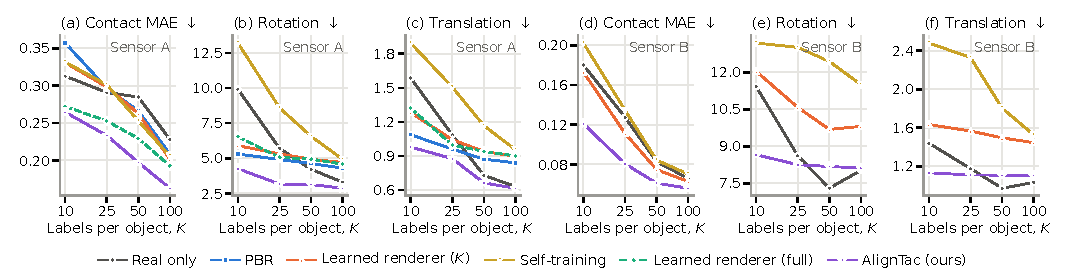
\includegraphics[width=0.9\textwidth]{figures/fig_kshot.pdf}
    \caption{\textbf{Label efficiency on two tactile sensors.} $K$: labeled training contacts per object. (a--c) Sensor-A validation, 150 epochs; the all-pairs (leaky) reference uses extra real labels and 50 epochs at $K=10$. (d--f) Sensor-B test, 50 epochs, renderer-free MeshTac. Matched methods share the registered contacts.}
    \label{fig:kshot}
\end{figure*}

\begin{table}[!htb]
\centering
\tableformat
\setlength{\tabcolsep}{3.0pt}
\begin{tabularx}{\columnwidth}{@{}rXrrrr@{}}
\toprule
$\Kreal$ & Method & \metrichead{Depth}{MSE} & \metrichead{Contact}{MAE} & \shortstack[c]{\strut IoU\\\strut $\uparrow$} & \metrichead{Rot.}{(deg)} \\
\midrule
\tabkshotshort
\bottomrule
\end{tabularx}
\caption{\textbf{Label-budget comparison on sensor A.} Validation: $472$ frames; $K$ labels per object. Self-training and MeshTac also use unlabeled images. Italic all-pairs rows exceed the budget ($K=10$: 50 epochs; others: 150). Matched rows use 150 epochs; bold marks the best at each $K$.}
\label{tab:kshot}
\end{table}

\subsection{Label Efficiency}
\label{sec:kshot}
We compare real-only training, learned-renderer augmentation, teacher-depth self-training and MeshTac using the same registered contacts at each $K$ (Table~\ref{tab:kshot}, Fig.~\ref{fig:kshot}). Self-training and MeshTac receive the same unlabeled training images; self-training applies pose supervision only to the registered subset.

At $K=25$, MeshTac lowers depth MSE by $19\%$ and contact MAE by $20\%$ relative to real-only training. Synthetic augmentation slightly improves all-pixel MSE but worsens contact MAE and IoU: lower MSE need not mean better contact reconstruction when background pixels dominate. Three-seed comparisons at 50 epochs confirm the MeshTac gain. MeshTac at $K=50$ also outperforms real-only training at $K=100$ in depth MSE ($0.0307$ versus $0.0369$), showing the value of aligned contacts beyond the registered set.

Removing the renderer preserves the depth improvement at every budget, supporting alignment as the main source of the within-session gain. Synthetic augmentation becomes useful for contact reconstruction at $K\ge50$ and under session changes (Sec.~\ref{sec:general}). Rotation improves for $K\le50$ but not at $K=100$; the reconstruction gain does not extend uniformly to pose.

\begin{table}[!htb]
\centering
\tableformat
\setlength{\tabcolsep}{1.8pt}
\resizebox{\columnwidth}{!}{%
\begin{tabular}{@{}lrrrrrrr@{}}
\toprule
& \multicolumn{3}{c}{Pseudo-labels vs.\ GT} & \multicolumn{4}{c}{Student validation} \\
\cmidrule(lr){2-4}\cmidrule(lr){5-8}
Pseudo-label & \shortstack[c]{\strut IoU\\\strut $\uparrow$} & \metrichead{Cont.}{MAE} & \metrichead{Rot.}{(deg)} & \metrichead{Depth}{MSE} & \metrichead{Cont.}{MAE} & \shortstack[c]{\strut IoU\\\strut $\uparrow$} & \metrichead{Rot.}{(deg)} \\
\midrule
\tabrcablmain
\bottomrule
\end{tabular}}
\caption{\textbf{Pseudo-label quality and student performance.} Sensor A, $K=25$, 50 epochs. Student results are three-seed means except \emph{Teacher depth + pose}. Withheld training GT scores labels only. $^{1/2}$ uses mesh depth for each object's half with lowest render error, teacher depth otherwise, and L1-search pose throughout. $\ddagger$ removes the renderer throughout the pipeline.}
\label{tab:abl}
\end{table}

\begin{figure}[t]
    \centering
    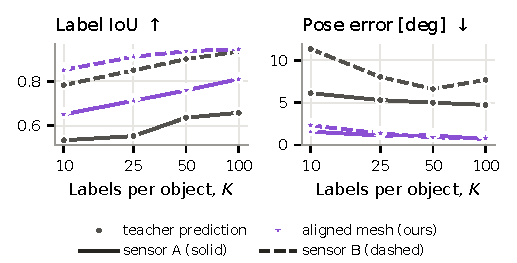
\includegraphics[width=\columnwidth]{figures/fig_labels.pdf}
    \caption{\textbf{Teacher and aligned-mesh label quality.} IoU, contact MAE and rotation error on unlabeled training images from both sensors, across label budgets $K$. Withheld GT is used only to evaluate the labels.}
    \label{fig:labels}
\end{figure}

\subsection{Ablation Study on Alignment Quality}
\label{sec:ablation}
We label the same unlabeled images with teacher predictions, L1 render-and-compare search or learned alignment, then evaluate both label quality and the student trained on those targets (Table~\ref{tab:abl}). Adding teacher pose isolates pose supervision; the renderer-free row additionally removes synthetic data.

Adding teacher pose mainly improves student rotation. Learned alignment improves label quality on both sensors (Fig.~\ref{fig:labels}) and raises student IoU from $0.624$ to $0.729$ relative to teacher-depth self-training. Correcting mesh placement therefore improves the supervision supplied to the student.

L1 search gives smaller gains. At $K=25$, the renderer assigns lower image error to the search-selected pose than to the GT pose on $93\%$ of frames. Thus, image similarity can favor a geometrically incorrect state; this statistic measures candidate ranking, not the search's pose-failure rate.

Gains persist with varied aligner settings and two random label selections; a second labeling round adds little. At $K=25$, $1.6\%$ of aligned sensor-A training poses exceed $5^\circ$ error, mostly on one nearly symmetric object. Translation errors follow repeated ridges, where different states can yield similar contact geometry.

\begin{figure*}[t]
    \centering
    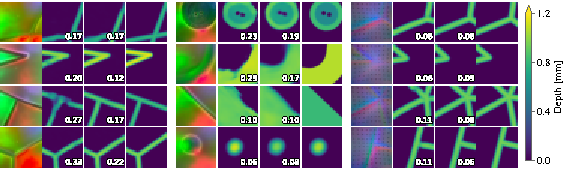
\includegraphics[width=0.8\textwidth]{figures/fig_qual.pdf}
    \caption{\textbf{Contact-depth reconstruction at $K=25$.} Each sensor shows three objects; each frame has its object's median contact-MAE improvement over real-only training. Numbers are contact MAE (mm), and depth maps share a color scale. Both displayed MeshTac models use synthetic data; the sensor-B curves in Fig.~\ref{fig:kshot}d--f use the renderer-free variant.}
    \label{fig:qual}
\end{figure*}

\begin{table}[!htb]
\centering
\tableformat
\setlength{\tabcolsep}{3pt}
\begin{tabularx}{\columnwidth}{@{}rXrr@{}}
\toprule
\multicolumn{4}{l}{\textbf{Sensor A: second-session evaluation}} \\
$\Kreal$ & Method & \metrichead{Contact}{MAE} & \shortstack[c]{\strut IoU\\\strut $\uparrow$} \\
\midrule
\tabcrossshortb
\midrule\midrule
\multicolumn{4}{l}{\textbf{Sensor B: sensor-specific training}} \\
$\Kreal$ & Method & \metrichead{Contact}{MAE} & \shortstack[c]{\strut IoU\\\strut $\uparrow$} \\
\midrule
\tabsbshortb
\bottomrule
\end{tabularx}
\caption{\textbf{Second-session and second-sensor results.} Top: sensor-A models tested on session 2 without retraining ($854$ frames). $\dagger$ uses all training labels from nine objects, with different object coverage from the $K$-shot rows. Bottom: models trained on sensor B and evaluated on its test set ($1{,}620$ frames); MeshTac is renderer-free. Sensor-B values are three-seed mean $\pm$ standard deviation. Contact MAE is in mm.}
\label{tab:general}
\end{table}

\subsection{Generalization Across Sessions and Sensors}
\label{sec:general}
\noindent\textbf{Second session.} We test sensor-A models on another day's contacts after object re-placement, without retraining (Table~\ref{tab:general}, top). MeshTac lowers contact MAE by $16\%$ at $K=25$ and $28\%$ at $K=100$ relative to real-only training. At $K=100$, synthetic augmentation improves on renderer-free MeshTac, which still outperforms self-training. At $K=25$, removing it gives slightly lower MAE ($0.306$ versus $0.310$). The benefit of simulation under this session change thus depends on the label budget.

\noindent\textbf{Second sensor.} We train each method separately on sensor B, keeping the aligner settings unchanged (Table~\ref{tab:general}, bottom). Renderer-free MeshTac lowers contact MAE by $36\%$ at $K=25$ and matches real-only training with twice as many labels. Three-seed checks at every budget support the gain, and evaluation with the original public labels gives the same qualitative result. At the other budgets, MeshTac lowers contact MAE by $15$--$33\%$, compared with at most $10\%$ from learned-renderer augmentation and no gain from self-training (Fig.~\ref{fig:kshot}e).

Figure~\ref{fig:qual} illustrates differences in ridge continuity and junction placement; quantitative comparisons use all evaluation frames.

\begin{table}[!htb]
\centering
\tableformat
\setlength{\tabcolsep}{3.5pt}
\begin{tabular}{@{}rrrrrrrrr@{}}
\toprule
& \multicolumn{4}{c}{Validation (session 1)} & \multicolumn{4}{c}{Session 2} \\
\cmidrule(lr){2-5}\cmidrule(lr){6-9}
& \multicolumn{2}{c}{Real only} & \multicolumn{2}{c}{MeshTac} & \multicolumn{2}{c}{Real only} & \multicolumn{2}{c}{MeshTac} \\
$\Kreal$ & pred. & +align & pred. & +align & pred. & +align & pred. & +align \\
\midrule
\tabposeref
\bottomrule
\end{tabular}
\caption{\textbf{Rotation error before and after mesh-assisted refinement.} Sensor A, mean error (deg) on session-1 validation and session-2 test images. \emph{pred.}: predictor output; \emph{+align}: six fixed-aligner iterations, without retraining.}
\label{tab:poseref}
\end{table}

\subsection{Mesh-Assisted Test-Time Pose Refinement}
\label{sec:tta}
We apply six fixed-aligner updates to real-only and MeshTac predictions using the test image and known mesh (Table~\ref{tab:poseref}). At $K\ge25$, both initializations reach $0.4$--$1.2^\circ$ mean rotation error within session 1: the aligner remains useful after student training and with a different predictor. At these budgets, session-2 means near $5^\circ$ exceed medians of $1.5$--$1.8^\circ$, motivating a confidence estimate to detect large residual errors.

\begin{table}[!htb]
\centering
\tableformat
\begin{tabularx}{\columnwidth}{Xrrrr}
\toprule
Method & \metrichead{Depth}{MSE} & \metrichead{Contact}{MAE} & \shortstack[c]{\strut IoU\\\strut $\uparrow$} & \metrichead{Rot.}{(deg)} \\
\midrule
\tabloomain
\bottomrule
\end{tabularx}
\caption{\textbf{Renderer baselines on held-out objects.} Sensor A, $1{,}244$ frames from three objects. Matched methods exclude their real contacts from training; simulation can use their meshes, except in the \emph{w/o held-out meshes} control. The italic leaky reference also uses real training pairs from these objects. Bold marks the best matched result.}
\label{tab:loo}
\end{table}

\subsection{Renderer Baselines: Unseen Objects and Label Leakage}
\label{sec:study}
We remove three objects from real training while allowing simulation to use their meshes (Table~\ref{tab:loo}). A control excludes those meshes as well. Simulated contacts lower rotation error from $64.7^\circ$ to $5$--$7^\circ$; removing the held-out meshes largely removes this gain. Dense MSE improves by at most $13\%$ among matched methods. In this setting, simulation provides more effective supervision for unseen-object pose than for dense reconstruction.

We then compare renderers trained on the same $K$ registered contacts with the all-pairs reference. The latter lowers MSE by $24$--$26\%$ in the few-label regime, but has access to additional real training labels. It represents a larger supervision budget; validation images remain excluded. Across 14 matched settings, contact-region image L1 correlates with downstream MSE ($\rho=0.95$). This supports its use for screening renderers, although the pooled correlation across budgets and variants does not establish causality or replace downstream evaluation.

\section{Discussion and Conclusion}

\noindent\textbf{Main findings.} MeshTac turns unlabeled real contacts into geometric supervision by aligning a known object mesh to each image. The ablations connect the improvement to the quality of this alignment: refining the contact state improves the projected labels, and the student trained on those labels reconstructs contact more accurately. Because the gain remains when synthetic images are removed, the evidence points to contact-state error---rather than appearance synthesis alone---as the main obstacle to using unlabeled contacts within a capture session.

\noindent\textbf{Lessons for label-efficient tactile learning.} Geometry coverage and sensor appearance play different roles. Real unlabeled images already provide the target appearance, so mesh alignment is a strong first step when registered contacts are scarce. Synthetic data becomes more useful when coverage changes, as seen in the second session and the unseen-object pose study. This suggests a practical order of operations: first establish a renderer-free alignment baseline, then add simulation when pose coverage or session robustness is limiting. Comparisons should disclose the real data used by the renderer, teacher and aligner, together with validation labels used for checkpoint selection; otherwise renderer supervision can be mistaken for a gain from simulation. Image fidelity can screen renderers, but downstream contact metrics remain necessary because lower all-pixel error need not mean better contact localization.

\noindent\textbf{Limitations and future work.} MeshTac assumes known objects: the predictor uses object identity, while pseudo-labeling and optional refinement require a mesh. The targets are mesh projections, so the experiments measure registered object geometry rather than physical elastomer deformation. The 12 ridge-pattern objects, labeled validation set and quasi-static presses leave curved and textured contacts, unknown objects, shear and slip untested. Repeated ridges also create translation ambiguity, and a small set of cross-session alignments retain large errors. Future work should develop uncertainty-aware or symmetry-aware alignment, extend the labels to dynamic contact, and test whether the geometric gains improve closed-loop manipulation. Relaxing the known-mesh assumption through joint shape and contact-state estimation is a further direction.


% The shorter sentence-case captions allow all table floats before the
% bibliography page; flushend can balance the final text columns normally.
\bibliographystyle{IEEEtran}
\bibliography{refs}

\end{document}
 for an author copy.
\ifdefined\MeshTacAuthorVersion
\author{I-Hsuan Huang$^{*}$, Xiaohao Xu$^{*}$, Xiangdong Wang, Xiaonan Huang, and Nima Fazeli%
\thanks{$^{*}$Equal contribution. All authors are with the University of Michigan, Ann Arbor, MI, USA.
Correspondence: \texttt{\{ihsuan, xiaohaox\}@umich.edu}.}%
}
\else
\author{Anonymous submission}
\fi
\hypersetup{pdfauthor={},pdftitle={MeshTac: Mesh-Aligned Pseudo-Labeling for Label-Efficient Tactile Geometry and Pose Estimation},pdfsubject={},pdfkeywords={}}

\begin{document}
\maketitle
\thispagestyle{empty}
\pagestyle{empty}\raggedbottom

\begin{abstract}
Dense geometric labels for vision-based tactile sensors come from pressing objects of known geometry at registered poses, so even with a mesh in hand, few real contacts are labeled. Simulation renders more image--label pairs from the mesh but must be calibrated or translated to the target sensor with real data, and self-training labels real images with a model's own predictions and inherits its errors. We observe that unlabeled tactile images already show the target appearance; what they lack is the contact pose that places the known mesh in them. MeshTac learns this registration from the few labeled contacts: a teacher proposes the pose, a residual aligner trained on perturbed labeled poses corrects it, and the aligned mesh provides depth, normal and pose labels for a student that predicts without the mesh. All trainable components share the same real labels. With 25 labels per object, MeshTac lowers contact depth error by $20\%$ and $36\%$ on two GelSlim-type sensors, matches real-only training with twice the labels, and keeps its gain without any renderer. Simulation looks far more useful when its renderer sees more real contacts than the predictor: a renderer trained on all real pairs reduces depth MSE by $24$--$26\%$, one restricted to the same 25 labels by $0$--$3\%$. The aligner also refines predicted poses at test time.
\end{abstract}

\section{Introduction}

Recovering contact geometry from touch gives a robot information about where an object meets its fingertip and how the object is oriented. Vision-based tactile sensors obtain this information by imaging the deformation of a soft elastomer. GelSight, GelSlim and DIGIT~\cite{yuan2017gelsight,donlon2018gelslim,lambeta2020digit} follow this principle, but their images differ with illumination, elastomer properties and camera response. Learning a geometric predictor requires examples of the target sensor's appearance together with accurate labels. We consider known-object perception: object identity and a mesh are available, but registering every captured contact to that mesh is costly.

\begin{figure*}[t]
    \centering
    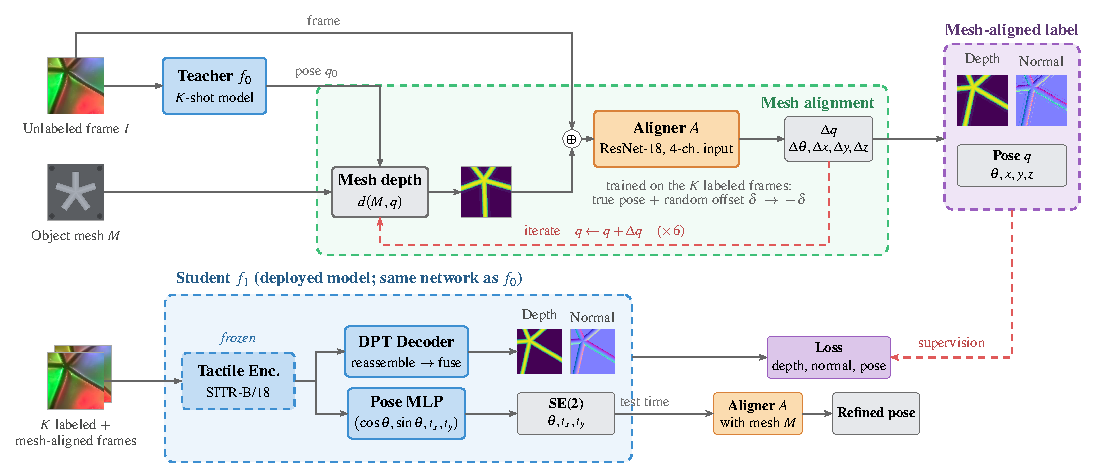
\includegraphics[width=0.97\textwidth]{figures/fig_arch.pdf}
    \caption{\textbf{Overview of MeshTac.} Teacher $f_0$ initializes the contact state. Aligner $A$ compares the frame with mesh depth and predicts a correction, applied six times. The aligned mesh supplies depth, normal and planar-pose targets for student $f_1$, which shares the teacher's architecture. All components use the same $K$ real training labels; the main sensor-A pipeline also uses synthetic examples, omitted here. The student requires no mesh at inference; optional pose refinement uses the image, mesh and fixed aligner. Blue: perception networks; orange: aligner; grey: geometry and pose; purple: labels and loss. Thumbnails show a $K=25$ example, including the student's actual prediction.}
    \label{fig:mapl}
\end{figure*}

Simulation can reduce the need for registered real contacts by generating tactile images and geometric labels from known meshes~\cite{wang2022tacto,si2022taxim,chen2023tacchi}. Its usefulness depends on whether the rendered appearance supports learning on the real sensor. Learned renderers can improve this correspondence, but training them also consumes real labels. A fair assessment of label efficiency must therefore count the supervision used by both the renderer and the downstream model.

Our renderer study exposes the importance of this accounting. A model augmented with images from a renderer trained on all real training pairs appears substantially more accurate than a model trained on a small labeled subset. Much of this advantage disappears when both components are restricted to the same subset: in the few-label regime on sensor A, learned rendering slightly lowers all-pixel depth error while worsening contact error and overlap. This finding motivates a more direct use of the mesh to supervise real images.

An unlabeled tactile image already contains the target sensor's appearance. If the object mesh is known, the missing information for a geometric label is its contact state: in-plane rotation, translation and indentation. A model trained on a small labeled set can initialize this state. Its estimate is often too imprecise to use directly, however, because pose errors shift the projected contact and corrupt the resulting dense labels. The central challenge is to align the mesh accurately enough for the additional images to become useful training data.

MeshTac addresses this challenge with a learned residual aligner (Fig.~\ref{fig:mapl}). Given a real image and mesh depth at a candidate state, the aligner predicts a correction. Perturbing the registered contacts supplies training examples without additional real labels. Unlike refinement used only at inference, MeshTac converts each corrected state into depth, normal and pose targets for training on real images. The student retains real contact appearance during training and predicts without a mesh at standard inference.

We evaluate MeshTac against real-only training, synthetic-data augmentation and teacher-based self-training under matched training-label budgets. Experiments with models trained separately for each sensor show that alignment improves both pseudo-label quality and the student's contact reconstruction. Renderer-free and second-session experiments distinguish the contribution of geometric supervision from that of synthetic appearance. Our contributions are:
\begin{itemize}
    \item \textbf{Mesh-aligned pseudo-labeling for known-object tactile perception.} MeshTac learns contact-state refinement from a small registered set and converts the refined meshes into consistent depth, normal and pose targets for unlabeled real images; the trained student remains mesh-free at standard inference.
    \item \textbf{Label accounting for tactile simulation.} A controlled study gives the renderer and downstream model the same real training-label budget, separating gains from synthetic data from gains obtained with additional paired real contacts.
    \item \textbf{Systematic empirical characterization.} Experiments with separately trained models on two sensors, a second capture session and held-out objects isolate the roles of alignment and synthetic data; they also evaluate reuse of the same aligner for optional test-time pose refinement without retraining.
\end{itemize}

\section{Related Work}

\noindent\textbf{Vision-based tactile sensing.}
GelSight-type sensors convert elastomer deformation into images under structured illumination~\cite{johnson2009retrographic,yuan2017gelsight}; GelSlim~\cite{donlon2018gelslim,sipos2024gelslim4} and DIGIT~\cite{lambeta2020digit} adapt the principle to fingertips. Because the measurement depends jointly on gel mechanics, LED layout and camera response, models transfer poorly between sensors; sensor-invariant representations~\cite{gupta2025sitr,zhao2024transferable,higuera2024sparsh,higuera2025sparshx} and deformation-space translation~\cite{zai2025across,yang2025flow} attack this on the representation side. We use a frozen sensor-invariant encoder~\cite{gupta2025sitr} as backbone so that our comparison isolates the data.

\noindent\textbf{Tactile simulation.}
Physically based tactile renderers synthesize GelSight images from mesh contacts~\cite{agarwal2021simulation,wang2022tacto,luu2023simulation}, with example-based~\cite{si2022taxim}, particle-based~\cite{chen2023tacchi}, differentiable~\cite{xu2022efficient} and GPU-scale~\cite{nguyen2024tacex,akinola2025tacsl} variants. Learned renderers instead map simulated depth or contact state to sensor images with an image-to-image network~\cite{isola2017pix2pix,church2022tactile,zhong2025tactgen}. Our two renderers follow the two lines and share meshes, contact sampler and labels, so they differ only in the appearance model.

\noindent\textbf{Unpaired refinement.}
When labeled real pairs are unavailable, synthetic images can be refined toward the real distribution with an adversarial loss on unlabeled real images: SimGAN~\cite{shrivastava2017simgan} adds a self-regularization term to keep the annotation valid, CycleGAN~\cite{zhu2017cyclegan} a cycle constraint, CUT~\cite{park2020cut} a patchwise contrastive constraint, and RCAN~\cite{james2019rcan} translates randomized renders to a canonical one. In tactile sensing, CycleGAN-based translation~\cite{chen2022cyclegan,jing2023uada}, SightGAN's background- and contact-reconstruction terms~\cite{azulay2024sightgan} and depth-conditioned diffusion~\cite{higuera2023braille} have been applied to GelSight-type sensors, evaluated on classification or contact position. These works do not state which real frames the translator saw relative to the test set, nor charge the translator's real data against the downstream budget. Self-training with pseudo labels~\cite{lee2013pseudo,xie2020noisy} is the standard way to use unlabeled data in vision; our mesh-aligned pseudo-labeling (Sec.~\ref{sec:mapl}) applies it to both sides of a real-to-sim-to-real pipeline, the renderer and the model, and replaces each pseudo label by the object mesh at a pose found with a learned residual aligner, as in iterative render-and-compare pose refinement~\cite{li2018deepim,wang2020self6d} but trained from the $\Kreal$ labeled tactile frames alone; our refiner (Sec.~\ref{sec:refiner}) adapts the unpaired family to the finding of this paper---geometry transfers, contact shading does not---by fixing the contact geometry through a mask composite and translating only the shading. Both are evaluated under the same leakage-controlled budget as the paired renderers.

\noindent\textbf{Sim-to-real transfer and its evaluation.}
Domain randomization~\cite{tobin2017domain,peng2018sim} and structured randomization around a calibrated center~\cite{chen2024general} trade fidelity for robustness; sensor-background conditioning~\cite{zhong2025tactgen} and low-fidelity pretraining~\cite{gano2025lowfidelity} report gains from synthetic tactile data. These works measure the benefit of simulation but rarely report how much real data the simulator consumed, or whether the simulator saw the test distribution. Cross-sensor transfer is usually attacked on the representation side~\cite{gupta2025sitr,zhao2024transferable}; we instead ask how much of a new sensor's or session's real data a renderer needs. No prior tactile study, to our knowledge, compares a physically calibrated and a learned renderer on the same meshes, contact sampler and downstream model, with the renderer's real data held disjoint from the test frames. Our contribution is this protocol---renderer and downstream model trained on the same disjoint real subset, tested on held-out objects, a second session and a second sensor---the resulting data-efficiency curves for depth, normals, pose and classification with both renderer families, and mesh-aligned pseudo-labeling, a self-training method with mesh-aligned pseudo labels that the curves motivate and that exceeds the leaky gain at $\Kreal=100$ from unlabeled frames.

\noindent\textbf{Pseudo-labeling and render-and-compare.}
Self-training on a model's own predictions~\cite{lee2013pseudo,xie2020noisy} is the standard way to use unlabeled data, but its labels inherit the model's errors. Object pose estimation refines a pose hypothesis by comparing a render of the model with the image, iteratively and with a learned update~\cite{li2018deepim}, and can self-supervise on unlabeled real images~\cite{wang2020self6d}. SnapTac brings the two together for tactile sensing: the pseudo label of a frame is not a network output but the object mesh at a pose found by a learned residual aligner, and the aligner is trained from the few labeled tactile frames alone, without a differentiable or photorealistic renderer.

\section{Method: Mesh-Aligned Pseudo-Labeling}
\label{sec:mapl}\label{sec:method}

\subsection{Problem Formulation}
We study how to learn tactile depth, normals and pose when object meshes are known but registered real contacts are scarce. The comparison includes synthetic-data augmentation and mesh-aligned pseudo-labeling, with real training labels shared across components.

A tactile renderer maps a mesh $\mathcal{M}$ and contact state $q$ (planar pose and indentation) to an image and dense labels, $(\hat{\mathcal{I}}, D, N) = \mathcal{R}_\theta(\mathcal{M},q)$. The geometry stage $(M,q)\mapsto(D,N)$ is shared by every renderer we study; renderers differ only in the appearance operator $\mathcal{P}_\theta:(D,N)\mapsto\hat{\mathcal{I}}$ and in the real data $\mathcal{D}^{r}_{\mathrm{cal}}$ used to fit $\theta$. A downstream model $f_\phi$ predicts depth, normals and planar pose from a real image. We measure a renderer by the real test error of $f_\phi$ trained on its synthetic data plus a real subset $\mathcal{D}^{r}_{\mathrm{task}}$, and we control the total real budget $\mathcal{D}^{r}_{\mathrm{cal}}\cup\mathcal{D}^{r}_{\mathrm{task}}$.

\subsection{Mesh-Aligned Pseudo-Labels}

\begin{figure}[t]
    \centering
    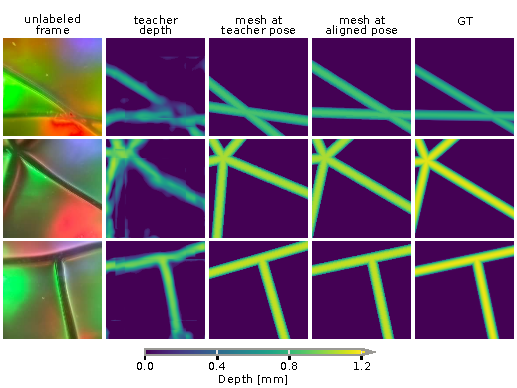
\includegraphics[width=\columnwidth]{figures/fig_align.pdf}
    \caption{\textbf{Pseudo-label construction.} Sensor A, $K=25$. Columns compare teacher depth and mesh projections before and after alignment with GT. Each row is a median-IoU example from a subsampled candidate set for one object. All depth maps use the same scale (mm).}
    \label{fig:align}
\end{figure}

AlignTac converts a small set of registered contacts and a larger pool of unlabeled real images into training data for a tactile predictor. The method first estimates each unlabeled contact state, then projects the known mesh to obtain mutually consistent depth, normal and pose targets.

\noindent\textbf{Geometric labels.} Let $d(\mathcal{M},q)$ denote the depth of object mesh $\mathcal{M}$ at contact state $q=(\theta,x,y,z)$, where $z$ is indentation. For a known object, these variables determine the mesh-derived depth map, its normals and the planar pose. Refinement therefore takes place in contact-state space, with the object geometry held fixed.

\noindent\textbf{Learning the aligner.} A ResNet-18, initialized from ImageNet, takes tactile RGB and candidate mesh depth as four input channels. It predicts a residual $A$ in contact-state units:
\begin{equation}
    \mathcal{A}\big(\mathcal{I},d(\mathcal{M},q^\ast+\delta)\big)\approx-\delta,
\end{equation}
where $q^\ast$ is the labeled state and $\delta$ is a sampled perturbation. The training set is produced by perturbing each registered contact, so learning the correction requires no labels beyond the original $K$ contacts. We normalize the residual dimensions and optimize a smooth-L1 loss; Sec.~\ref{sec:setup} gives the perturbation ranges and training details.

\noindent\textbf{Labeling real images.} For each unlabeled training image, teacher $f_0$ initializes planar pose and sets indentation to its maximum predicted depth. Given the known mesh, we perform six updates,
\begin{equation}
    q_{t+1}=q_t+\mathcal{A}\big(\mathcal{I},d(\mathcal{M},q_t)\big),
\end{equation}
clipping indentation to $[0.3,1.6]\,$mm. The final mesh depth, normals and planar pose label the image. We retain every pseudo-labeled training frame in the evaluated configuration (Sec.~\ref{sec:ablation}).

\noindent\textbf{Training the student.} Student $f_1$ has the teacher's architecture and learns from the $K$ labeled frames and the mesh-aligned frames. Synthetic frames from a renderer may be added as a separate variant; AlignTac itself uses none. Pseudo-labels are generated exclusively from the training split.

\noindent\textbf{Optional test-time refinement.} The student predicts from an image without mesh rendering. When the object identity and mesh are available, the same fixed aligner can refine its predicted pose using the test image. We evaluate this additional inference step separately in Sec.~\ref{sec:tta}.

\section{Experimental Setup}
\label{sec:setup}

\begin{figure}[t]
    \centering
    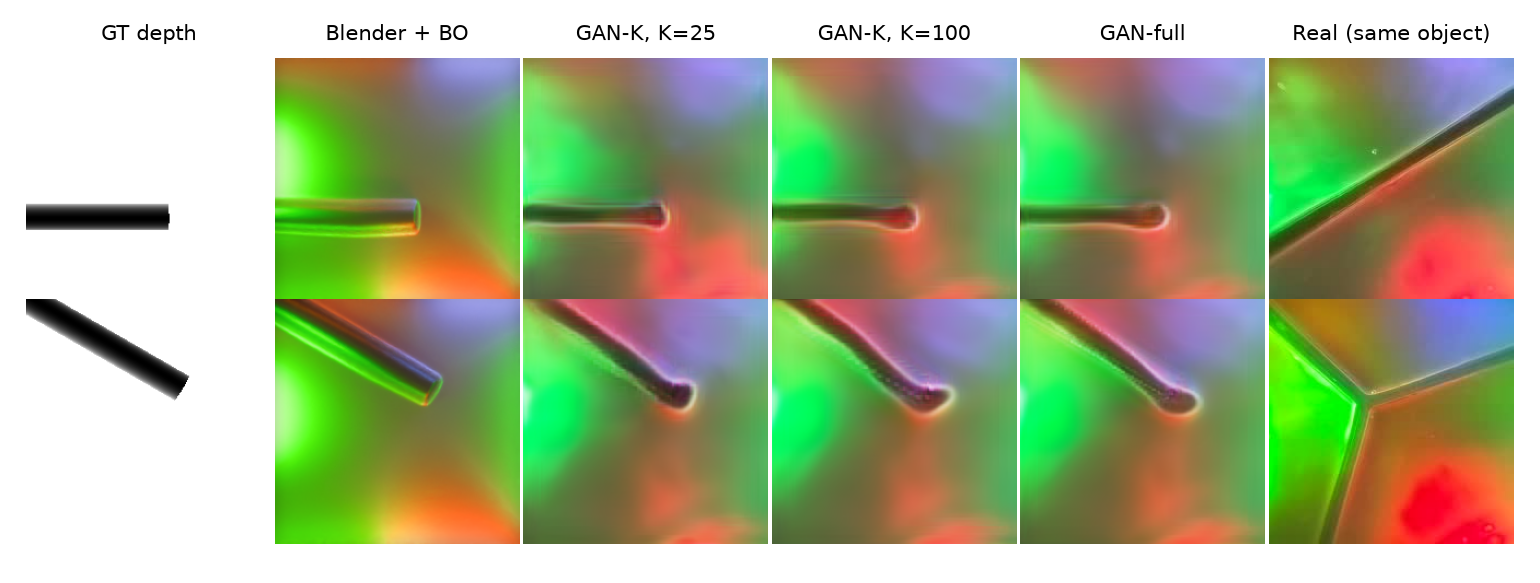
\includegraphics[width=\columnwidth]{figures/long/fig_renders.png}
    \caption{\textbf{Two renderers, one contact.} Each row is one simulated contact (GT depth, left) rendered by the physically calibrated Blender renderer, by the learned renderer trained on $\Kreal=25$ or $\Kreal=100$ real pairs per object, and by the learned renderer trained on all real pairs (GAN-full). Right: a real frame of the same object. PBR reproduces the illumination field but not the dark contact shading of the real gel; the learned renderers reproduce the shading and inherit the illumination of their training frames.}
    \label{fig:renders}
\end{figure}

\subsection{Sensors and Data}
\noindent\textbf{Sensor A.} Sensor A is GelSlim~5.0~\cite{wang2026gelslim}, a marker-free design with a $17.5\,$mm square gel view imaged under six colored LED emitters. Images are center-cropped to $0.816$ of the view and resized to $224\times224$.

\noindent\textbf{Real data (session 1).} A KUKA LBR Med arm presses the sensor onto 12 objects of known geometry, recording the image and end-effector pose at every contact; ground-truth (GT) depth and normals are the mesh projected at the recorded pose (geometric targets, not membrane measurements). After removing frames whose image contact region disagrees with the GT, $4{,}669$ frames remain ($222$--$568$ per object), one session per object, every tenth frame held out as validation ($472$ frames).

\noindent\textbf{Real data (session 2).} The same objects were re-placed and re-captured on another day (48 runs). GT poses were re-estimated per frame by maximizing the IoU between the image ridge mask and the projected mesh contact and manually reviewed; the curated test set has $854$ frames of $11$ objects (Sec.~\ref{sec:cross}). The session-1 calibration no longer held after re-placement (per-run corrections averaged $11^\circ$ and $1.6\,$mm). Apart from the label-free adaptation study of Sec.~\ref{sec:cross}, which trains on images from half of the session-2 presses without their poses and tests on the other half, nothing from this session is used for training or model selection.

\noindent\textbf{Sensor B.} Sensor B is GelSlim~4.0~\cite{sipos2024gelslim4}, with a marker array, a different illumination layout and a $12\,$mm field of view. Its public depth dataset~\cite{sipos2024gelslim4} has the same 12 objects pressed by a parallel gripper at $1\,$mm indentation with mesh-derived depth and in-hand pose labels ($135$ test frames per object). We use the left finger, the central $12\times12\,$mm, and report rotation after removing a per-object constant offset because its pose origin differs from ours.

The public depth labels are clipped at the nominal indentation and smoothed, so they are not exact mesh projections. For the AlignTac comparisons in Sec.~\ref{sec:sensorb}, a global search fits the planar mesh pose to each public label ($0.018\,$mm mean residual). We canonicalize the fitted pose using the object's rotational symmetry and use its projected mesh depth for training and testing (\emph{mesh-fitted} labels). A separate set of renderer experiments in Sec.~\ref{sec:sensorb} retains the original public labels; those results are identified explicitly.

\noindent\textbf{Contact sampler.} For each object we sample contact cells over the mesh at 12 base rotations ($30^\circ$ apart), an indentation of $0.8$--$1.2\,$mm and in-plane jitter, and export $D$ from the object z-buffer and $N$ by finite differences. Simulated poses are restricted to each object's real rotation and translation ranges. The same $5{,}345$ simulated contacts feed every renderer.

\subsection{Physically Calibrated Renderer}
\label{sec:blender}
The physically based renderer (PBR) is implemented in Blender/Cycles: a gel surface mesh is shrink-wrapped onto the object and smoothed (35 corrective iterations), shaded with a glossy/transparent material and a height-driven contact-darkening term, lit by six area emitters, and post-processed (saturation, brightness, contrast, haze, a low-frequency random gel warp). Emitter and post-processing parameters (16 scalars) are fitted by tree-based Bayesian optimization of an $L_2$ plus histogram distance between the real and rendered no-contact image (500 evaluations); gel and contact parameters were hand-tuned by visual comparison with a single separately captured calibration contact of one object, which is not among the held-out objects. Thus, the renderer sees one no-contact image and one contact image, without depth or pose labels; neither is counted in the label budget.

\noindent\textbf{Domain-randomization baseline.} To test whether careful calibration is necessary, we also render with randomized sensor parameters: random HSV colors and strengths for each LED emitter, random gel optics, per session, with the geometry stage (scale, field of view, smoothness) fixed. This variant uses no image to fit its randomized appearance parameters; it retains the shared geometry configuration.

\subsection{Learned Renderer}
\label{sec:gan}
The learned renderer is a conditional GAN~\cite{isola2017pix2pix}: a five-level U-Net that takes the depth map and two coordinate channels and outputs an RGB image, a $70\times70$ spectral-normalized PatchGAN discriminator, and an adversarial $+\,100\,(\mathrm{L1} + \mathrm{gradient\;L1} + \mathrm{low\text{-}frequency\;L1})$ loss. Simulated depth is jittered by $\pm15\%$ at generation time.

\noindent\textbf{Real budget.} GAN-$\Kreal$ is trained on $\Kreal$ real (depth, image) pairs per object, an evenly spaced subset of each object's training frames that is \emph{the same} $\Kreal$ frames the downstream model receives; GAN-LOO on all training frames of the 9 non-held-out objects; GAN-full on all $4{,}197$ pairs in the legacy protocol, or on the $3{,}667$ pairs that exclude the held-out test frames in the clean protocol. Small budgets train for at least $30$k generator updates.

\noindent\textbf{Variants.} \emph{Background-conditioned}: the session's no-contact image is appended as three input channels, providing session illumination from one background frame. \emph{Physics-conditioned}: PBR's image of the same contact is appended, optionally predicting only a residual on top of it, optionally with the background. \emph{Difference image}: the target is the image minus the session background. \emph{Blender-pretrained}: pretraining on $30$k (depth, Blender image) pairs, then fine-tuning on the real pairs.

\emph{Multi-sensor}: the background-conditioned GAN is trained on 100 simulated sensor designs (random LED layouts and gel materials) plus optionally the target sensor's real pairs; this tests whether sensor diversity can replace sensor-specific real data. \emph{Rotation coverage} changes the geometry stage instead: we vary how many of an object's real rotations appear in simulation (1, 2 or all 12) and, for the learned renderer, rotate the depth map before rendering so that every rotation is covered.

\subsection{Zero-Label Alternative: Contact-Preserving Unpaired Refiner}
\label{sec:refiner}
We also test whether unlabeled real images can improve synthetic appearance without paired renderer supervision. Following unpaired image translation~\cite{shrivastava2017simgan,park2020cut,chen2022cyclegan}, we train a refiner to change the shading of a physical render while preserving its contact region. The refiner $\mathcal{F}$ takes the physical render $\hat{\mathcal{I}}_{\mathrm{phys}}$, the session background $B$ and the contact mask $m$ (simulated depth $>0$, dilated by 4\,px and feathered) and outputs
\begin{equation}
    \hat{\mathcal{I}} = m \odot \mathcal{F}(\hat{\mathcal{I}}_{\mathrm{phys}}, B, m) + (1-m) \odot B ,
\end{equation}
The background is therefore taken from the real sensor, while the refiner changes only the contact region. Depth, normal and pose targets remain those of the physical render.

 $\mathcal{F}$ is the same U-Net as the learned renderer with a 7-channel input. It is trained against a $70\times70$ PatchGAN on \emph{unlabeled} real frames (image only; no depth, no pose) with an adversarial loss and a patchwise contrastive loss (PatchNCE~\cite{park2020cut}) between the encoder features of input and output, sampled preferentially inside $m$, to encourage preservation of the rendered ridge structure. We train for 10k generator updates with batch size 8 and Adam ($2\times10^{-4}$, $\beta_1=0.5$).

Its real budget is the set of unlabeled frames plus one background frame per session, and the same leakage rule applies: in leave-object-out the held-out objects' frames are excluded, in $\Kreal$-shot the same $\Kreal$ frames as the downstream model are used without their labels. With domain-randomized inputs, the refiner requires no appearance calibration or paired training labels; it retains the shared geometry configuration.

\subsection{Downstream Tactile Model}
The downstream model is identical for every renderer: a frozen sensor-invariant encoder (SITR-B/18~\cite{gupta2025sitr}) provides patch tokens at four depths; a DPT decoder~\cite{ranftl2021dpt} predicts depth and normals at $224\times224$; a pose head regresses $(\cos\theta,\sin\theta,t_x,t_y)$ from the class token and mean patch token. For the classification study, we add a 12-class head (LayerNorm on concatenated class and mean patch tokens, two-layer MLP with GELU) and train with cross-entropy alongside the other losses. The decoder, pose head and object embedding are trained ($12$M parameters). Losses are MSE on depth and normals, $1-\cos(\theta-\hat\theta)$ on rotation and L1 on translation, balanced by grouped uncertainty weighting~\cite{kendall2018multi}.

When synthetic data is used, training mixes simulated and real frames. Simulated frames receive photometric augmentation and $\pm15^\circ$ gel-spin rotation with matched labels; real frames are not augmented. We use AdamW with learning rate $2\times10^{-4}$, batch size 32 and a cosine schedule. Main sensor-A runs use 150 epochs, while sensor B and seed/ablation studies use 50. Depth and normal metrics use the checkpoint with the lowest validation depth MSE (at $K\le25$ within the first ten epochs). Pose metrics use the checkpoint with the lowest validation rotation error in every table and figure, including the session-2, sensor-B and test-time refinement evaluations; the pose head does not overfit (final-epoch and selected-epoch rotation agree within $0.3^\circ$), whereas rotation at the early dense checkpoint mainly reflects its short training. Translation error is the mean absolute error over the two coordinates. In every case, checkpoint selection uses validation labels in addition to the $K$ training labels.

\subsection{AlignTac Implementation}
Aligner perturbations span $\pm8^\circ$, $\pm1.5\,$mm in-plane and $\pm0.15\,$mm in indentation; half use ranges scaled by $0.3$. Training uses smooth L1 for 8,000 steps (batch 64, AdamW, learning rate $3\times10^{-4}$). Aligners train on real examples only, the teacher uses the $K$ real frames, and the student receives no synthetic frame. The \emph{+ learned synth.} variant (sensor A) mixes 24 real and 40 synthetic examples generated by the $K$-pair renderer in each aligner batch, trains the teacher with learned-renderer data, and gives the student synthetic images from a renderer retrained on labeled and aligned real pairs.

On one RTX 6000 Ada GPU, aligner training takes about $20$ minutes, labeling $0.5\,$s per frame ($30$ minutes for the $3{,}897$ sensor-A frames), and student training $1.3$ hours for 50 epochs or $2.2$ hours for 150. The renderer, when used, adds about one hour.

\subsection{Data-Access Protocol}
\label{sec:protocol}
Paired renderers and the aligner exclude validation and test images from training. The $K$-shot protocol additionally limits paired training labels to the same $K$ frames per object. Validation labels remain available for model selection; the reported budget counts training labels. Physical-renderer manual tuning is described separately above.

\noindent\textbf{Two evaluation protocols.} The headline sensor-A results (Table~\ref{tab:kshotT}, Table~\ref{tab:rcablT}, the test-time alignment table and Figs.~\ref{fig:kshot}, \ref{fig:conv} and \ref{fig:qual}) follow a clean protocol: $530$ session-1 frames (every tenth and every eighth-of-ten frame that is not among the $K$ labeled contacts) are held out from all training, including renderer fitting and pseudo-labeling, and every number is reported on them; the $472$ validation frames are used only for checkpoint selection. The extended variant tables (Tables~\ref{tab:kshot}--\ref{tab:rcabl}, \ref{tab:cross}, \ref{tab:selection} and \ref{tab:variants}) predate this split and report the legacy protocol, in which models were selected and evaluated on the same validation frames; they are kept for the additional variants they cover and are marked as such. Under both protocols the conclusions are identical.

\noindent\textbf{Leave-object-out (LOO).} Three objects (a two-line, a rod and a cross pattern; $1{,}244$ frames) are removed from all real training, excluded from paired-renderer and aligner training, and evaluated in full. Simulated contacts of the three meshes are available to every renderer (``new object with a CAD model but no real touches''). A \emph{geometry control} additionally removes the three meshes from simulation.

\noindent\textbf{$\Kreal$-shot.} Every object contributes $\Kreal\in\{0,10,25,50,100\}$ evenly spaced real training frames. For $K>0$, the learned renderer is trained on exactly those frames; the downstream model co-trains on them plus simulated data, or on them alone with the same number of updates. Evaluation is on the real validation split. The aligner of AlignTac receives the same $\Kreal$ frames, and the remaining training frames may be used \emph{without} their labels.

\noindent\textbf{Cross-session and cross-sensor.} Session-2 and sensor-B test frames are never used to train or select anything in the sensor-A study. In the sensor-B study the $\Kreal$-shot protocol is repeated with sensor-B real pairs and the sensor-B test split.

\noindent\textbf{Learned renderer (full).} GAN-full is trained on all sensor-A training pairs ($4{,}197$ in the legacy protocol; $3{,}667$ in the clean protocol, which excludes the held-out test frames). In LOO, these include real pairs from held-out objects; in $K$-shot, they include training labels withheld from budget-matched methods, but no validation frames. We label this non-comparable reference ``learned renderer (full)''; it is shown in italics and excluded from best-result highlighting.

\noindent\textbf{Metrics.} We report depth MSE over all pixels ($\mathrm{mm}^2$), following prior work on this sensor. Because $\approx90\%$ of pixels are background, we also report mean absolute error inside the GT contact region (contact MAE, mm) and contact IoU (predicted depth $>0.05\,$mm vs.\ GT $>0$), which also penalizes false contact. Normals are evaluated by mean angular error inside the contact region (deg), and pose by mean rotation error (deg) and translation error (mm; mean absolute error over the two coordinates).

\section{Experiments}
\label{sec:exp}\label{sec:experiments}

All numbers are errors on real frames of the downstream model after 150 epochs (50 where noted); depth MSE in $\mathrm{mm}^2$, contact MAE in mm, normals and rotation in degrees. Sections~\ref{sec:kshot}--\ref{sec:qual} evaluate MAPL; Sections~\ref{sec:loo}--\ref{sec:fidelity} report the leakage-controlled renderer study that provides its baselines.


\begin{figure*}[t]
    \centering
    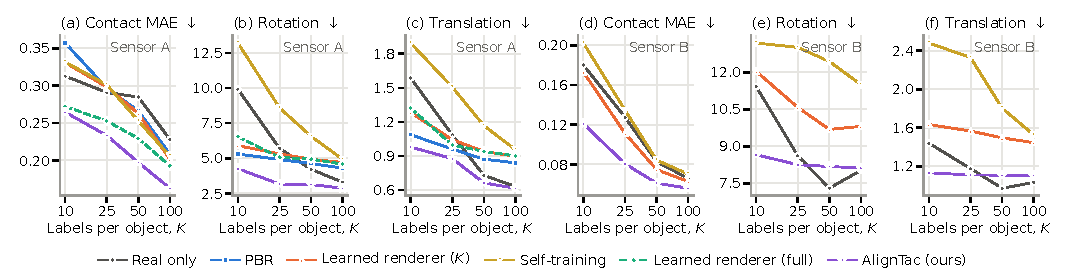
\includegraphics[width=0.95\textwidth]{figures/fig_kshot.pdf}
    \caption{\textbf{Label efficiency} (real validation error vs.\ labeled frames per object). The leakage-free learned renderer separates from real-only training only at $\Kreal=50$ and the physical renderer never improves dense error, while the leaky renderer (dashed) appears to help everywhere. MAPL improves dense error at every budget and passes the leaky renderer at $\Kreal=100$.}
    \label{fig:kshot}
\end{figure*}

\begin{table}[!tbp]
\centering
\tableformat
\caption{\textbf{$\Kreal$-shot with a shared real budget.} Every object contributes $\Kreal$ real frames; GAN-$\Kreal$ is trained on the same frames. MAPL and self-trained rows additionally use the unlabeled training frames (Sec.~\ref{sec:unlabeled}); refiner rows use no label at all. Real validation split ($472$ frames). Leaky rows use the renderer trained on all real pairs (the $\Kreal=10$ leaky row is a 50-epoch run).}
\label{tab:kshot}
\begin{tabularx}{\columnwidth}{lXrrrrr}
\toprule
$\Kreal$ & Training data & \metrichead{Depth}{MSE} & \metrichead{Contact}{MAE} & \shortstack[c]{\strut IoU\\\strut $\uparrow$} & \metrichead{Normal}{(deg)} & \metrichead{Rot.}{(deg)} \\
\midrule
\tabkshot
\bottomrule
\end{tabularx}
\end{table}

\subsection{Label Efficiency}
\label{sec:kshot}
Table~\ref{tab:kshot} and Fig.~\ref{fig:kshot} compare, at equal label budget, real-only training, co-training with either renderer, self-training on the teacher's own predictions (Sec.~\ref{sec:ablation}) and MAPL. Each MAPL run uses the $2{,}997$--$4{,}077$ training frames outside the $\Kreal$ budget without their labels.

\noindent\textbf{Simulation alone.} Neither leakage-free renderer improves dense error for $\Kreal\le25$; the learned renderer helps from $\Kreal=50$ (depth MSE $-10\%$, $-16\%$ at $\Kreal=100$), the physical renderer by at most $5\%$. Both lower rotation error at $\Kreal=10$ ($9.6^\circ\!\to\!5$--$6^\circ$) and raise it at $\Kreal=100$.

\noindent\textbf{MAPL} improves on real-only training at every budget: depth MSE by $13\%$, $19\%$, $36\%$ and $37\%$ and contact MAE by $13\%$, $20\%$, $27\%$ and $28\%$ at $\Kreal=10$, $25$, $50$ and $100$, with IoU $+0.06$ to $+0.08$ and normal error $-2.6^\circ$ to $-5.1^\circ$. Over three seeds (50 epochs) the depth MSE is $0.0558\pm0.0003$, $0.0447\pm0.0009$, $0.0313\pm0.0007$ and $0.0229\pm0.0003$ against $0.0635\pm0.0007$, $0.0551\pm0.0010$, $0.0480\pm0.0006$ and $0.0366\pm0.0008$ for real-only training. Three comparisons put the gain in perspective. MAPL with $50$ labels per object ($0.0307$) is ahead of real-only training with $100$ ($0.0369$) and on par with the learned renderer at $100$ ($0.0311$). At $\Kreal=100$ it is \emph{better} than the leaky renderer (depth MSE $0.0232$ vs.\ $0.0274$, contact MAE $0.168$ vs.\ $0.205$), and at $\Kreal=25$ it matches the leaky contact MAE and IoU at $8\%$ higher depth MSE. Its rotation error is the lowest leakage-free value for $\Kreal\le50$ ($4.0^\circ$, $3.7^\circ$, $3.7^\circ$); at $\Kreal=100$ real-only training is ahead ($3.2^\circ$ vs.\ $3.7^\circ$) until the aligner is also used at test time (Sec.~\ref{sec:tta}). MAPL does not need the renderer for these numbers: with a real-only teacher, an aligner trained on the $\Kreal$ frames alone and no synthetic frame at all (``no renderer''), depth MSE is $0.0521$, $0.0433$, $0.0291$ and $0.0227$ and rotation error $2.5$--$4.7^\circ$, equal to or better than with the renderer; the renderer earns its place across sessions (Sec.~\ref{sec:cross}).

\begin{table}[!tbp]
\centering
\tableformat
\caption{\textbf{Seeds.} Mean $\pm$ standard deviation over three seeds (50 epochs) on the real validation split. ``+ MAPL'': real-only teacher, no synthetic frame; ``with renderer'': the configuration of Table~\ref{tab:kshot}.}
\label{tab:seeds}
\setlength{\tabcolsep}{2.0pt}
\footnotesize
\begin{tabularx}{\columnwidth}{@{}rXcccc@{}}
\toprule
$\Kreal$ & Training data & Depth MSE & Cont.\ MAE & IoU & Rot. \\
\midrule
\tabseeds
\bottomrule
\end{tabularx}
\end{table}

\noindent\textbf{Seeds.} Table~\ref{tab:seeds} repeats the main comparison with three seeds: the standard deviations are an order of magnitude below the differences between methods.

\begin{table}[!tbp]
\centering
\tableformat
\caption{\textbf{Alignment ablation} ($\Kreal=25$, 50 epochs; first, fifth and last row are three-seed means). Left: quality of the pseudo labels of the unlabeled frames against their withheld true labels (evaluation only). Right: real validation error of the model trained on them. Depth label: teacher prediction or mesh depth at the fitted pose ($^{1/2}$: mesh on the half of each object's frames with the lowest render error, teacher on the rest). Pose label: none (pose loss on the $\Kreal$ labeled frames only), teacher pose, pose found by L1 render-and-compare search with GAN-$\Kreal$ ($^{1/2}$: on the confident half only), or the learned aligner. $\ddagger$: synthetic data from the teacher-pair renderer; $\dagger$: MAPL (renderer retrained on the aligned pairs).}
\label{tab:rcabl}
\setlength{\tabcolsep}{3pt}
\resizebox{\columnwidth}{!}{%
\begin{tabular}{@{}llrrrrrrr@{}}
\toprule
\multicolumn{2}{c}{Labels of $U$} & \multicolumn{3}{c}{Pseudo-label quality} & \multicolumn{4}{c}{Downstream} \\
\cmidrule(lr){1-2}\cmidrule(lr){3-5}\cmidrule(lr){6-9}
Depth & Pose & \shortstack[c]{\strut IoU\\\strut $\uparrow$} & \metrichead{Cont.}{MAE} & \metrichead{Rot.}{(deg)} & \metrichead{Depth}{MSE} & \metrichead{Cont.}{MAE} & \shortstack[c]{\strut IoU\\\strut $\uparrow$} & \metrichead{Rot.}{(deg)} \\
\midrule
\tabrcabl
\bottomrule
\end{tabular}}
\end{table}

\begin{figure}[!tbp]
    \centering
    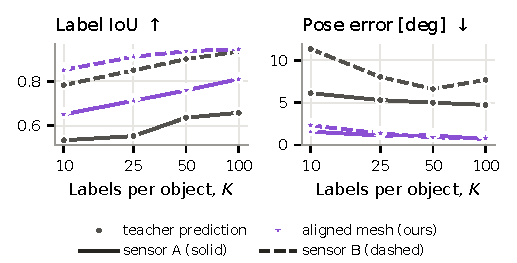
\includegraphics[width=\columnwidth]{figures/fig_labels.pdf}
    \caption{\textbf{Label quality on the unlabeled frames} against their withheld reference labels (evaluation only): the $\Kreal$-shot teacher's own prediction versus the mesh at the aligned pose. The aligner improves on the teacher at every budget on both sensors.}
    \label{fig:labels}
\end{figure}

\subsection{Why Alignment: Ablation}
\label{sec:ablation}\label{sec:unlabeled}
Table~\ref{tab:rcabl} varies only how the unlabeled frames are labeled.

\noindent\textbf{Self-training.} With the teacher's own depth as label (stitched from five windows to cover the full frame, pose loss on the labeled frames only), depth MSE improves by $8\%$ but contact MAE and IoU do not: the pseudo labels inherit the teacher's localization error (label IoU $0.56$), so the student learns sharper depth values, not where the contact is. Adding the teacher's pose as a label restores rotation accuracy and nothing else, and a second round of self-training changes depth MSE by at most $4\%$ in either direction.

\noindent\textbf{L1 render-and-compare.} Replacing the aligner by a search---fit the mesh to the teacher depth on a pose grid, then pick, among $567$ neighbouring poses, the one whose GAN-$\Kreal$ render is closest to the frame in image L1---helps less (label IoU $0.64$, pose error $2.5^\circ$) and requires gating: on the half of the frames with the larger render error the mesh label is no better than the teacher's. The few-shot renderer is a poor comparator; at $\Kreal=25$ its render at the true pose is farther from the frame than its render at the selected pose on $93\%$ of the frames.

\noindent\textbf{Learned aligner.} The aligner lowers the teacher's pose error from $5.3^\circ$ to $1.1^\circ$ on the $3{,}897$ unlabeled frames and yields labels with IoU $0.71$ and contact MAE $0.24\,$mm (teacher: $0.55$, $0.32$). Label quality grows with the budget (IoU $0.65$, $0.71$, $0.76$, $0.81$ and pose error $1.6^\circ$, $1.1^\circ$, $1.1^\circ$, $0.7^\circ$ for $\Kreal=10$--$100$). The student trained on these labels is the first to lower contact error ($0.310\!\to\!0.246$) and to raise IoU ($0.624\!\to\!0.729$). Further findings: (i) the aligner is learned from the $\Kreal$ real frames---adding frames rendered by GAN-$\Kreal$ at random poses does not change label quality (IoU $0.72$), and training on such renders alone fails ($0.56$); (ii) no gate is needed, since on the frames a render-error gate would reject its labels still beat the teacher's (IoU $0.66$ vs.\ $0.55$); (iii) it is insensitive to its settings (half or double the perturbation range: $0.72$, $0.73$; 2k or 20k steps: $0.73$, $0.72$; ResNet-34 or -50 backbone: $0.73$, $0.71$), while dropping the ImageNet initialization costs accuracy ($0.67$); (iv) the student is unchanged whether its synthetic frames come from the renderer retrained on aligned pairs or on teacher-labeled pairs (depth MSE $0.0447$ in both cases), and within the session it does not need them at all (last row: $0.0433\pm0.0004$ over three seeds with a real-only teacher and no synthetic frame, against $0.0447\pm0.0009$ with the renderer); (v) a quarter of the unlabeled frames already gives most of the gain (depth MSE $0.0453$, $0.0452$ and $0.0447$ with $25\%$, $50\%$ and $100\%$ of $U$), while IoU keeps growing with their number ($0.710$, $0.725$, $0.729$); (vi) a second round, with the student as the new teacher, does not improve further: although the student proposes poses $1.5^\circ$ closer than the original teacher, the aligned labels (IoU $0.65$, $0.71$ at $\Kreal=10$, $25$) and the retrained student (depth MSE $0.0570$, $0.0445$; IoU $0.674$, $0.717$) are within seed variation of the first round. An unpaired sim-to-real refiner of the physical render, which uses the unlabeled frames without any pose, does not improve on its input (contact MAE $0.349$ vs.\ $0.346$ on unseen objects).

\noindent\textbf{Self-trained renderer.} Following self-training~\cite{lee2013pseudo,xie2020noisy}, the $\Kreal$-shot downstream model pseudo-labels $U$ (depth predicted on five windows and stitched back to the full frame; frames kept when the predicted contact overlaps the image's black-hat ridge mask, IoU $\ge0.2$: $3{,}260$ frames at $\Kreal=25$, $2{,}677$ at $\Kreal=100$), and GAN-$\Kreal$ is retrained on the $\Kreal$ true plus the pseudo pairs. The pseudo labels are as accurate as the labeler ($0.32$ and $0.24\,$mm contact MAE against the withheld true labels), and the renderer's fidelity improves by $5\%$ at both budgets ($0.108\!\to\!0.102$, $0.077\!\to\!0.073$), which the proxy translates into a $1\%$ downstream gain: depth MSE $0.0544\!\to\!0.0538$ at $\Kreal=25$ and $0.0311\!\to\!0.0308$ at $\Kreal=100$ (contact MAE $0.207$, the best leakage-free value at $\Kreal=100$). With teacher labels the renderer thus gains little from more real images. With the aligned pairs of step~2 it gains more: contact-region error falls by $13$--$19\%$ at every budget ($0.121\!\to\!0.105$ at $\Kreal=10$, $0.108\!\to\!0.090$ at 25, $0.095\!\to\!0.077$ at 50, $0.077\!\to\!0.065$ at 100; leaky $0.057$), the best strict renderers of the study, although swapping this renderer for the teacher-pair one leaves the downstream error of the aligned model unchanged (Table~\ref{tab:rcabl}): once the real frames carry good labels, the synthetic frames matter little.

\noindent\textbf{Window stitching.} Without alignment the label is the teacher depth, and labeling $U$ on the center window alone leaves the pseudo depth empty outside the $0.816$ crop (pseudo-label contact MAE $0.41\,$mm over the full frame instead of $0.32$). The self-trained model then has the same depth MSE ($0.0518$ vs.\ $0.0517$, model only, $\Kreal=25$; Table~\ref{tab:kshot}) but a worse contact MAE ($0.328$ vs.\ $0.300$) and a $30\%$ larger peak-depth error, and the gap persists across sessions (contact MAE $0.358$ vs.\ $0.318$): the rotation augmentation brings the frame border into the training crop, where unstitched labels are wrong.

\noindent\textbf{Rounds.} Without alignment, relabeling $U$ with $f_1$ and repeating the renderer and model steps improves the pseudo labels at $\Kreal=25$ (label IoU $0.56\!\to\!0.60$, contact MAE $0.32\!\to\!0.31\,$mm, $3{,}516$ frames kept instead of $3{,}260$) but not at $\Kreal=100$ ($0.66\!\to\!0.65$), and the downstream change is small in both directions: depth MSE $0.0508\!\to\!0.0500$ and IoU $0.628\!\to\!0.642$ at $\Kreal=25$, $0.0285\!\to\!0.0295$ and $0.750\!\to\!0.736$ at $\Kreal=100$, rotation unchanged ($6.2^\circ$, $4.9^\circ$). The labeler's localization error is not something its own student can correct; the alignment step is. With alignment a second round changes nothing either (item (vi) above): one round of MAPL saturates.

\begin{table}[!tbp]
\centering
\tableformat
\caption{\textbf{Cross-session.} Sensor-A models evaluated on the curated session-2 set ($854$ frames, 11 objects; poses re-estimated per frame and manually reviewed). Rot.: raw; Rot.$^{\ast}$: after removing a per-object constant offset (the re-placement of the object). All models use the full session-1 real set unless a $\Kreal$ is given.}
\label{tab:cross}
\begin{tabularx}{\columnwidth}{Xrrrrr}
\toprule
Training data & \metrichead{Contact}{MAE} & \shortstack[c]{\strut IoU\\\strut $\uparrow$} & \metrichead{Normal}{(deg)} & \metrichead{Rot.}{(deg)} & \metrichead{Rot.$^{\ast}$}{(deg)} \\
\midrule
\tabcross
\bottomrule
\end{tabularx}
\end{table}

\subsection{A Second Session}
\label{sec:cross}
On the second session (Table~\ref{tab:cross}) dense error is $1.5$--$3\times$ the same-session value, partly because the reference poses are re-estimated. The ordering of the methods is preserved. MAPL has the lowest contact MAE and the highest IoU of its budget ($0.310$, $0.660$ at $\Kreal=25$; $0.252$, $0.743$ at $\Kreal=100$), i.e.\ $16\%$ and $28\%$ less contact error than real-only training, as within the session; at $\Kreal=100$ it is ahead of the model trained on \emph{all} session-1 labels ($0.315$, $0.675$) and level with that model's leaky variant. Simulation also helps across sessions (contact MAE $0.315\!\to\!0.27$--$0.29$ and rotation $16.4^\circ\!\to\!10.5$--$11.5^\circ$ for the full-data model). Here the synthetic frames matter: without the renderer MAPL loses its advantage over self-training at $\Kreal=100$ (contact MAE $0.288$, IoU $0.707$), although it is as accurate within the session---the renderer's contribution is robustness to the appearance of a new session, consistent with Sec.~\ref{sec:study}. Raw rotation error remains above $10^\circ$ for every method because the objects were re-placed; two thirds of it is a per-object constant.

\noindent\textbf{Renderer baselines across sessions.} Table~\ref{tab:cross} evaluates the sensor-A models on the second capture. Dense error is $1.5$--$3\times$ the same-session value (e.g.\ contact MAE $0.315\,$mm against $0.117$ for the model trained on all session-1 real data), partly because the reference poses are re-estimated; the informative quantity is the ordering. Simulation helps every task across sessions. With the full session-1 real set, contact MAE falls from $0.315\,$mm (real only) to $0.29$ with the physical and $0.27$ with the learned renderer, IoU rises from $0.675$ to $0.69$--$0.70$ and $0.72$--$0.73$, normal error falls from $25.4^\circ$ to $24.0$--$24.9^\circ$ with the calibrated and learned renderers, and raw rotation error drops from $16.4^\circ$ to $9.7$--$11.5^\circ$; the geometry control ($28.7^\circ$) shows that the pose gain again comes from mesh coverage. The domain-randomized renderer matches the calibrated one on dense error ($0.294$, IoU $0.691$) and is slightly behind on pose ($12.3^\circ$), as on unseen objects: randomized appearance degrades the contact-silhouette signal. About $2/3$ of the remaining rotation error is a per-object constant (Rot.$^{\ast}$ $4.7$--$6.5^\circ$ for every model), i.e.\ the re-placement offset rather than a perception error. In the $\Kreal$-shot regime the dense gain grows with $\Kreal$: at $\Kreal=25$ only the learned renderer lowers contact MAE ($0.368\!\to\!0.342$), at $\Kreal=100$ both renderers do ($0.351\!\to\!0.295$--$0.299$) and the learned one also raises IoU ($0.657\!\to\!0.713$) and lowers rotation error ($17.5^\circ\!\to\!13.7^\circ$), whereas simulation-only training does not transfer dense geometry across sessions (IoU $0.56$, normal $51^\circ$): the session-invariant part of the synthetic data is its geometry, not its appearance.

\begin{table}[!tbp]
\centering
\tableformat
\caption{\textbf{Test-time alignment.} Rotation error (deg) of the predicted pose and after six aligner iterations against the object mesh. No retraining.}
\label{tab:poseref}
\setlength{\tabcolsep}{3.5pt}
\begin{tabular}{@{}rrrrrrrrr@{}}
\toprule
& \multicolumn{4}{c}{Validation (session 1)} & \multicolumn{4}{c}{Session 2} \\
\cmidrule(lr){2-5}\cmidrule(lr){6-9}
& \multicolumn{2}{c}{Real only} & \multicolumn{2}{c}{MAPL} & \multicolumn{2}{c}{Real only} & \multicolumn{2}{c}{MAPL} \\
$\Kreal$ & pred. & +align & pred. & +align & pred. & +align & pred. & +align \\
\midrule
\tabposeref
\bottomrule
\end{tabular}
\end{table}

\subsection{Test-Time Alignment}
\label{sec:tta}
Since pose is defined with respect to a known object, the $\Kreal$-shot aligner can refine the pose predicted on a test frame (Table~\ref{tab:poseref}). On the validation split rotation error falls from $3.2$--$9.6^\circ$ to $0.4$--$2.8^\circ$ for real-only models and from $3.7$--$4.0^\circ$ to $0.8$--$1.5^\circ$ for MAPL models; from $\Kreal=25$ on the refined error is about $1^\circ$ whichever model proposes the pose, and translation error falls by $25$--$50\%$. On the second session rotation error falls from $13$--$20^\circ$ to $5$--$11^\circ$ (real only) and from $9$--$11^\circ$ to about $5^\circ$ (MAPL) with a median of $1.5$--$2.2^\circ$: the mean is dominated by a minority of frames on which the alignment fails. The mesh at the aligned pose is also a depth estimate: on the validation split it is as accurate as the MAPL student's output (IoU $0.81$ vs.\ $0.79$, contact MAE $0.158$ vs.\ $0.168\,$mm at $\Kreal=100$) and lifts a real-only model to the MAPL level (IoU $0.656\!\to\!0.710$ at $\Kreal=25$), so the student distills into a mesh-free network what alignment achieves with the mesh. The aligner also generalizes across objects: trained on the nine seen objects of the leave-object-out protocol and applied to the three held-out ones, whose only available data is their mesh, it lowers the rotation error of the simulation-trained models of Table~\ref{tab:loo} from $4.8$--$6.8^\circ$ to $0.6$--$1.0^\circ$.

\begin{table}[!tbp]
\centering
\tableformat
\caption{\textbf{Second sensor (\sensorB{}) with mesh-registered labels}; $1{,}620$ test frames, 50 epochs. ``no renderer'': real-only teacher and no synthetic frame. Self-training uses the teacher's own depth as label.}
\label{tab:sbmapl}
\setlength{\tabcolsep}{2.4pt}
\begin{tabularx}{\columnwidth}{@{}rXrrrrr@{}}
\toprule
$\Kreal$ & Training data & \metrichead{Depth}{MSE} & \metrichead{Contact}{MAE} & \shortstack[c]{\strut IoU\\\strut $\uparrow$} & \metrichead{Normal}{(deg)} & \metrichead{Rot.}{(deg)} \\
\midrule
\tabsbmapl
\bottomrule
\end{tabularx}
\end{table}

\subsection{A Second Sensor}
\label{sec:sensorb}
\noindent\textbf{MAPL.} On \sensorB{} ($1{,}620$ test frames) MAPL transfers without any change of settings (Table~\ref{tab:sbmapl}, Fig.~\ref{fig:kshot}d). The public depth labels of this dataset are not mesh projections, so we re-registered them: the mesh pose that best explains each label was fitted ($0.018\,$mm mean residual) and canonicalized against the object's rotational symmetry, and every method was retrained and tested on these mesh-registered labels. The few-shot teacher is already accurate on this sensor (label IoU $0.78$, $0.85$, $0.90$, $0.93$ on the unlabeled frames at $\Kreal=10$, $25$, $50$, $100$; $0.55$ at $\Kreal=25$ on sensor A), yet the aligner improves on it at every budget (IoU $0.85$, $0.91$, $0.94$, $0.95$; pose error $2.3^\circ$, $1.4^\circ$, $0.9^\circ$, $0.8^\circ$ against $6.6$--$11.4^\circ$). At $\Kreal=25$ the student lowers depth MSE from $0.0179\pm0.0004$ to $0.0075\pm0.0001$ and contact MAE from $0.127\pm0.001$ to $0.078\pm0.0003\,$mm over real-only training (three seeds) and raises IoU from $0.849$ to $0.903$. The baselines gain far less: the learned renderer trained on the $25$ pairs reaches $0.111\,$mm (IoU $0.877$) and self-training on the teacher's depth does not improve on real data ($0.135\,$mm, $0.846$). Without any synthetic frame, MAPL lowers contact MAE from $0.180$, $0.127$, $0.083$, $0.066$ to $0.121$, $0.081$, $0.061$, $0.056\,$mm at $\Kreal=10$--$100$ ($-15$ to $-36\%$) and depth MSE by $33$--$58\%$, so that, as on sensor A, it needs about half the labels of real-only training for a given contact error. Rotation error improves at $10$ and $25$ labels ($14.0^\circ\!\to\!9.5^\circ$, $13.4^\circ\!\to\!9.2^\circ$) but not beyond ($9^\circ$ either way). Scored against the original public labels, MAPL keeps its advantage (contact MAE $0.137\!\to\!0.098\,$mm at $\Kreal=25$).

\begin{table}[!tbp]
\centering
\tableformat
\caption{\textbf{Sensor B (\sensorB{}).} $1{,}620$ test frames of the same 12 objects. Top: sensor-A models applied zero-shot. Below: models trained on $\Kreal$ sensor-B real frames per object, alone, with the sensor-A physical renderer, with a learned renderer trained on the same $\Kreal$ sensor-B pairs, or with self-training on teacher labels (MAPL without its alignment step, Sec.~\ref{sec:mapl}; labeler: the GAN-25 model; 50 epochs). Rotation after removing a per-object offset.}
\label{tab:sensorb}
\begin{tabularx}{\columnwidth}{lXrrrrr}
\toprule
$\Kreal$ & Training data & \metrichead{Depth}{MSE} & \metrichead{Contact}{MAE} & \shortstack[c]{\strut IoU\\\strut $\uparrow$} & \metrichead{Normal}{(deg)} & \metrichead{Rot.}{(deg)} \\
\midrule
\tabsensorb
\bottomrule
\end{tabularx}
\end{table}

\noindent\textbf{Renderer baselines (original labels).} Sensor B has a marker array, a different LED layout and a smaller field of view (Table~\ref{tab:sensorb}). \emph{Zero-shot}, sensor-A models recover contact only partially (IoU $0.28$ for the all-real model, $0.37$ for the simulation-only model: the model trained on the most sensor-A real data transfers worst) and rotation not at all (residual $\approx11.5^\circ$ for every model, the value a constant predictor attains on the $\pm22.5^\circ$ label range). \emph{With sensor-B real pairs}, the $\Kreal$-shot picture of Sec.~\ref{sec:kshot} reappears: a learned renderer trained on the sensor's own $\Kreal=25$ pairs lowers contact MAE from $0.139$ to $0.100\,$mm ($-29\%$), normal error from $17.2^\circ$ to $14.6^\circ$ and raises IoU from $0.82$ to $0.85$; at $\Kreal=10$ the gain is $6\%$, at $\Kreal=100$ real data alone is already at $0.058\,$mm and simulation neither helps nor hurts dense error. The sensor-A physical renderer, calibrated to a different sensor, still helps at $\Kreal=25$ ($0.125$) but less; the domain-randomized renderer matches it ($0.126$) without using any real data from either sensor. At $\Kreal=100$ real data alone is already at $0.058\,$mm and simulation neither helps nor hurts dense error; the domain-randomized renderer ($0.062$) is close. Rotation is not improved by either renderer and is degraded at $\Kreal=100$ ($7.5^\circ\!\to\!9$--$10^\circ$), as on sensor A. The transition is earlier on sensor B ($\Kreal\approx25$ vs.\ $50$), plausibly because its uniform $1\,$mm indentation and larger contact regions make the depth-to-image mapping easier to learn from few pairs.

\noindent\textbf{Self-training (original labels).} With the original labels and the GAN-25 model as labeler, teacher-label self-training lowers depth MSE from $0.0152$ (real only) to $0.0098$ and contact MAE from $0.140$ to $0.100\,$mm at $\Kreal=25$ without synthetic data, i.e.\ it reaches its labeler ($0.0107$, $0.100$) but does not pass it in contact error; with the mesh-registered labels and a real-only teacher it does not improve on real data at all (Table~\ref{tab:sbmapl}). In both protocols the student inherits the localization of its labeler, which is what alignment corrects.

\begin{figure*}[t]
    \centering
    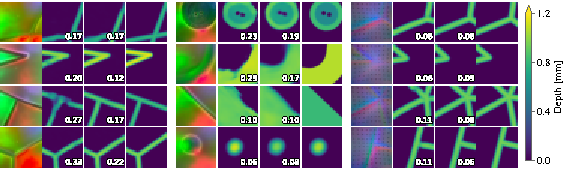
\includegraphics[width=0.97\textwidth]{figures/fig_qual.pdf}
    \caption{\textbf{Predictions on held-out frames} ($\Kreal=25$): real-only training versus MAPL on both sensors, with the per-frame contact MAE. For each object the frame shown is the one whose improvement is the object's median improvement.}
    \label{fig:qual}
\end{figure*}

\subsection{Qualitative Results}
\label{sec:qual}
Fig.~\ref{fig:qual} shows predictions at $\Kreal=25$ on held-out frames of both sensors; for every object the displayed frame is the one with the object's median improvement in contact MAE, so the examples are representative rather than selected. Real-only models blur or break thin ridges and misplace junctions; the MAPL student recovers their extent and position. On sensor B the real-only model is already close and the gain shows at junctions and at the ends of ridges.

\begin{table}[!tbp]
\centering
\tableformat
\caption{\textbf{Leave-object-out.} Errors on $1{,}244$ real frames of three objects with no real training data. Rows add simulated contacts of all 12 meshes to the real frames of the nine other objects, unless noted. The multi-sensor row is a 50-epoch run. Normal error is inside the contact region. Bold: best leakage-free.}
\label{tab:loo}
\begin{tabularx}{\columnwidth}{Xrrrrrr}
\toprule
Training data & \metrichead{Depth}{MSE} & \metrichead{Contact}{MAE} & \shortstack[c]{\strut Contact\\\strut IoU\,$\uparrow$} & \metrichead{Normal}{(deg)} & \metrichead{Rot.}{(deg)} & \metrichead{Trans.}{$L_1$} \\
\midrule
\tabloo
\bottomrule
\end{tabularx}
\end{table}

\subsection{Baseline Study: Unseen Objects}
\label{sec:loo}
Three objects are removed from all real training while their meshes remain available to simulation (Table~\ref{tab:loo}).

\noindent\textbf{Pose.} Without any data of the three objects the pose head is at chance ($64.7^\circ$). Simulated contacts of the three meshes bring it to $6.8^\circ$ with the physical renderer---calibrated from one no-contact frame and never shown a real contact---and to $5.7^\circ$ with the strict learned renderer; the leaky renderer ($4.6^\circ$) buys little, and the geometry control (same renderer, meshes removed) stays at $50.6^\circ$. Pose transfer is geometric coverage; any renderer that preserves the contact silhouette suffices. Replacing the calibrated renderer with domain-randomized sensor parameters (random LED colors and strengths, gel optics randomized per session, geometry pinned) gives $8.9^\circ$, between the calibrated ($6.8^\circ$) and single-rotation ($10.3^\circ$) rows; calibration helps by providing a consistent appearance from which the encoder extracts geometry.

\noindent\textbf{Rotation coverage.} How much of the pose space must simulation cover? Restricting simulation to one real rotation per object leaves $10.3^\circ$, two rotations $7.5^\circ$, all twelve $6.8^\circ$ (Blender rows of Table~\ref{tab:loo}); rendering the learned renderer's inputs after rotating the depth map (rotate-then-render) gives the best leakage-free pose, $4.4^\circ$. Coverage of the rotation range, not the number of synthetic frames, is the operative variable.

\noindent\textbf{Depth and normals.} Contact MAE on the unseen objects is $0.36\,$mm for real-only training, three times the seen-object value; the plain renderers reduce it by at most $4\%$ and the geometry control by almost as much ($0.340$), so this is regularization by extra frames, not object coverage. The domain-randomized Blender renderer improves contact MAE to $0.342$ and IoU to $0.601$, matching the calibrated renderer ($0.346$, $0.592$), suggesting that appearance diversity from randomized sensor parameters acts as regularization even without calibration data. A multi-sensor GAN trained on 100 simulated sensor designs does not improve over single-sensor baselines ($0.358$, $0.579$); mixing simulated sensors cannot replace real pairs. The one leakage-free renderer that helps significantly is the background-conditioned GAN-LOO: depth MSE $-13\%$, contact MAE $0.323$, IoU $0.633$, for one background frame per session; it remains far from the leaky reference ($-30\%$), which has seen real contacts of the objects. Normal error follows contact MAE. Peak-depth error is $0.05$--$0.08\,$mm for every row: the models estimate \emph{how deep} correctly and err in \emph{where} the contact lies.

\noindent\textbf{Object classification.} We add a 12-class classification head (LayerNorm + MLP on the class and mean patch tokens) and train with cross-entropy. With real data of the nine objects, the model classifies them at $94\%$ validation accuracy, but the three held-out objects score $0\%$---even when simulation provides their contact patterns through either the calibrated or learned renderer. Pose estimation transfers to unseen objects through geometry, but classification requires the appearance of the real contact, which no leakage-free renderer reproduces.

\subsection{Baseline Study: Real-Data Budget of a Renderer}
\label{sec:budget}
Table~\ref{tab:kshot} and Fig.~\ref{fig:kshot} vary the real budget of the renderers. Three regimes appear.

\noindent\textbf{Zero-shot.} Simulation alone transfers poorly for dense geometry (contact MAE $0.41\,$mm vs.\ $0.11$ with the full real set); the leaky renderer halves this but has seen $4{,}197$ real pairs.

\noindent\textbf{Few-shot ($\Kreal\le25$).} Neither leakage-free renderer improves dense error. At $\Kreal=25$ GAN-25 lowers depth MSE by $3\%$ ($0.0536\pm0.0013$ vs.\ $0.0551\pm0.0010$ over seeds) but not contact MAE or IoU; the physical renderer does the same. With $\Kreal\le25$ the real training loss reaches $10^{-4}$ within ten epochs while validation error is flat from epoch five: the model memorizes the few real frames, and synthetic frames with a different contact appearance do not regularize that memorization. Simulation does help pose at $\Kreal=10$ ($9.6^\circ\!\to\!5.2$--$5.9^\circ$), as in Sec.~\ref{sec:loo}.

\noindent\textbf{Moderate budget ($\Kreal\ge50$).} The learned renderer now helps: at $\Kreal=50$ depth MSE $0.0482\!\to\!0.0434$ ($-10\%$), contact MAE $0.283\!\to\!0.260$, IoU $0.69\!\to\!0.72$; at $\Kreal=100$ depth MSE $0.0369\!\to\!0.0311$ ($-16\%$; $0.0366\!\to\!0.0299$ over seeds, $-18\%$), contact MAE $0.235\!\to\!0.210$, IoU $0.74\!\to\!0.77$, and normal error improves in step. The physical renderer gives $-1$ to $-5\%$ MSE. The learned renderer thus needs $\approx\!50$ labeled contacts per object before its data is worth more than the frames it was trained on, and at every $\Kreal\ge50$ simulation \emph{worsens} rotation by $0.2$--$1.3^\circ$.

\subsection{Leakage, a Fidelity Proxy, and Negative Results}
\label{sec:fidelity}\label{sec:study}
\noindent\textbf{Cost of leakage.} Across Tables~\ref{tab:loo} and \ref{tab:kshot} the leaky renderer reports depth MSE reductions of $24$--$31\%$ at every budget and on unseen objects; the strict numbers are $0$--$3\%$ for $\Kreal\le25$, $10$--$16\%$ at $\Kreal\ge50$ and $5$--$13\%$ on unseen objects. The bias is largest where the pipeline is most attractive---few or no real contacts of the target---because the leaky renderer has memorized the test contacts (it reproduces validation frames with a contact-region L1 of $0.057$, half that of any strict renderer).

\begin{figure}[!tbp]
    \centering
    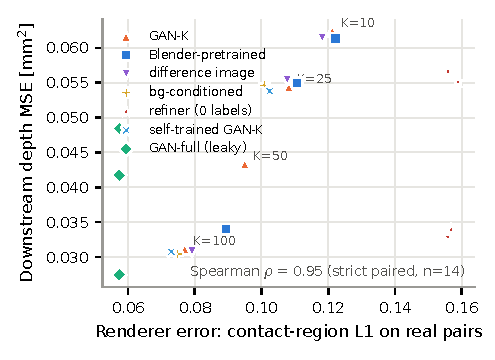
\includegraphics[width=0.85\columnwidth]{figures/fig_fidelity.pdf}
    \caption{\textbf{Renderer fidelity predicts downstream error.} Contact-region L1 between rendered and real images on held-out real (depth, image) pairs versus depth MSE of the downstream model trained with that renderer's data, for every learned-renderer variant and budget.}
    \label{fig:fidelity}
\end{figure}

\noindent\textbf{A fidelity proxy.} Rendering the depth maps of the real validation pairs and comparing with the real images gives an image error per renderer. Fig.~\ref{fig:fidelity} plots the contact-region L1 against the downstream depth MSE for every learned-renderer variant: the ordering is preserved across variants and budgets. Over the strict paired renderers, pixel metrics predict downstream error best (Spearman $|\rho|$: contact L1 $0.95$ over the 14 renderers of Fig.~\ref{fig:fidelity}, $0.97$ over the nine original ones; PSNR $0.98$, full-image L1 $0.95$), perceptual metrics worse (SSIM $0.87$, LPIPS $0.87$, contact-cropped $0.90$); adding the three leaky renderers, whose fidelity is identical while their downstream error varies with $\Kreal$, lowers every correlation to $0.75$--$0.82$, i.e.\ fidelity predicts the renderer's contribution, not the real budget. The unpaired refiner is the one exception: it is scored against the gel-warped physics render rather than its own input, so its contact L1 ($0.16$) is not comparable (Sec.~\ref{sec:unlabeled}). The proxy costs seconds and screened the variants below before downstream training.

\begin{table}[!tbp]
\centering
\tableformat
\caption{\textbf{Appearance-side and training-side variants} at $\Kreal=25$ (real validation split) and leave-object-out (unseen objects). Fidelity is the contact-region L1 of Fig.~\ref{fig:fidelity}; physics-guided variants were stopped at the fidelity stage. Only the background-conditioned renderer improves unseen-object depth.}
\label{tab:variants}
\begin{tabularx}{\columnwidth}{Xrrrrr}
\toprule
& \multicolumn{2}{c}{$\Kreal=25$} & \multicolumn{3}{c}{Unseen objects} \\
\cmidrule(lr){2-3}\cmidrule(lr){4-6}
Variant & \shortstack[c]{\strut Fidelity\\\strut $\downarrow$} & \metrichead{Contact}{MAE} & \shortstack[c]{\strut Fidelity\\\strut $\downarrow$} & \metrichead{Contact}{MAE} & \metrichead{Rot.}{(deg)} \\
\midrule
\tabvariants
\bottomrule
\end{tabularx}
\end{table}

\noindent\textbf{Which factor limits few-shot fidelity?}

Table~\ref{tab:variants} tests the hypotheses.
\emph{(i) Missing physical prior.} Pretraining the GAN on $30$k Blender pairs, conditioning it on the Blender image of the same contact, predicting a residual on top of that image, or conditioning on Blender image and background all leave contact-region fidelity unchanged or worse at $\Kreal\in\{10,25\}$ (the physical renderer's random gel-warp of $\pm3$ pixels means the conditioning image is not pixel-aligned with the target, which may limit this family).
\emph{(ii) Session illumination drift.} Session backgrounds differ by $0.05$--$0.10$ L1, more than the best renderer's total error ($0.03$); normalizing frames to a canonical background or predicting difference images improves full-image L1 by $13$--$21\%$ but leaves contact-region L1 and contact MAE unchanged (the frozen encoder is robust to the illumination field). Conditioning the renderer on the background does help on unseen objects (Sec.~\ref{sec:loo}) because it lets a renderer that never saw the object reproduce its session's illumination.
\emph{(iii) Training-side changes.} A contact-mask head with a gradient-matching loss, Blender pretraining followed by real fine-tuning, and fine-tuning with an L2-SP anchor change $\Kreal=25$ contact MAE by at most $\pm0.02\,$mm.
\emph{(iv) Domain randomization.} Randomizing the sensor's LED colors, strengths and gel optics per session while keeping the geometry stage fixed (Table~\ref{tab:variants}, ``domain rand.'') matches the calibrated renderer's contact MAE at $\Kreal=25$ ($0.320$ vs.\ $0.329$) and on unseen objects ($0.342$ vs.\ $0.346$). On sensor B at $\Kreal=25$ the match is even closer ($0.126$ vs.\ $0.125$). The calibrated renderer's advantage on pose ($6.8^\circ$ vs.\ $8.9^\circ$ on unseen objects) is consistent with a less noisy silhouette. Domain randomization is thus a viable zero-cost baseline when calibration data is not available, but it cannot close the gap to the learned renderer.
\emph{(v) Contact shading.} What remains is the appearance \emph{inside} the contact (Fig.~\ref{fig:renders}), and every result is consistent with it being the limit: strict renderers separate from real-only training only after enough contacts, leakage helps exactly because it exposes the test contacts, classification never transfers (the identity features lie entirely in the contact shading), and the residual errors are localization rather than depth-magnitude errors.

\noindent\textbf{Unpaired refiner (0 labels).} The contact-preserving refiner of Sec.~\ref{sec:refiner} translates the physical render using only unlabeled frames. On unseen objects (Table~\ref{tab:loo}) it does not improve on the calibrated render (contact MAE $0.349$ vs.\ $0.346$; on the domain-randomized render $0.353$), and its self-regularized variant is slightly worse ($0.360$): without a single labeled pair the adversarial objective is satisfied by any plausible contact shading, including a fainter one, and the ridge structure that geometry transfer needs is not what the discriminator judges. In the $\Kreal$-shot protocol, refining with the same $\Kreal=25$ frames used as unlabeled images gives the best leakage-free dense numbers at that budget (contact MAE $0.297$, IoU $0.672$, normal $27.1^\circ$; Table~\ref{tab:kshot}), a $5\%$ contact-MAE gain where no paired renderer helps, while using all of $U$ ($0.309$) or $\Kreal=100$ ($0.224$ vs.\ real-only $0.235$, GAN-100 $0.210$) adds little. The refiner's contact-region L1 ($0.156$--$0.159$, against the $\pm3\,$px-warped physics render whose identity score is $0.179$) is not comparable to the paired renderers' and is excluded from Fig.~\ref{fig:fidelity}.

\noindent\textbf{Mixing the two renderers.} Alternating physical and learned frames (Blender$\,\oplus\,$GAN) yields the average of the two on dense error and the better of the two on pose ($5.6^\circ$ on unseen objects, equal to GAN-LOO; $9.8^\circ$ across sessions, the lowest of all renderers except background normalization), so a practitioner who has both should mix them for pose and rely on the learned one for depth.

\section{Discussion, Limitations and Conclusion}

\noindent\textbf{Practical recipe.}
For a new tactile sensor and known object meshes, first select a small set of registered contacts spanning the intended contact states. Reserve a separate labeled validation set and report its size alongside the training budget. Train a teacher and a residual aligner on the available training labels; use the aligner to assign mesh-derived depth, normal and pose targets to additional real images. Train a student on the labeled and aligned frames. On our objects, one alignment round without confidence filtering is sufficient; repeated rounds give little further improvement.

The renderer-free pipeline is a useful starting point: it retains the within-session depth gains and avoids appearance-model training. When the deployment session differs from the training session, our results support adding synthetic data from a renderer retrained on the labeled and aligned real pairs. At $K=100$ on sensor A, this lowers second-session contact MAE from $0.288$ to $0.252\,$mm. If real contacts of a new object are unavailable but its mesh is known, synthetic pose coverage is also useful: the held-out-object study reduces rotation error from $64.7^\circ$ to $5$--$7^\circ$. Optional test-time alignment can further refine pose when object identity and mesh are available, but its larger residuals across sessions should be considered for the intended application. These recommendations concern the evaluated ridge-pattern contacts; they do not establish a universal label threshold for other sensors or geometries.

\noindent\textbf{Reporting.}
Report the real data used by every component, including the renderer, teacher, aligner and checkpoint-selection procedure. Distinguish labeled training pairs, unlabeled images, validation labels and images inspected during manual calibration. A renderer fitted to all available training pairs can exceed a downstream $K$-shot budget without seeing a validation image. In leave-object-out evaluation, access to real images of the held-out objects is a separate protocol violation. Both should be distinguished from access to the held-out meshes, which is permitted in our geometry-transfer study.

Under this accounting, the all-pairs renderer's $24$--$26\%$ depth-MSE reduction over $K$-shot real-only training is a result at a larger label budget, not a gain from simulation at a cost of $K$ labels. Report metrics that distinguish depth magnitude from contact localization, since all-pixel MSE can improve while contact MAE or IoU worsens. Also identify training duration, seed aggregation, checkpoint selection and test-time mesh use. Contact-region rendering error can help screen appearance models, but its observed correlation with downstream error pools multiple budgets and renderer variants; it should complement downstream evaluation rather than replace it.

\noindent\textbf{Limitations.} MeshTac requires the identity and mesh of each object during pseudo-labeling and optional test-time refinement. Our evaluation covers 12 ridge-pattern objects and does not establish performance on curved or textured contacts, unknown objects, or a manipulation task. GT is mesh-derived on both sensors; sensor-B targets are re-registered public labels. Validation labels are also needed for checkpoint selection. Alignment can fail, particularly across sessions, and repeated ridge patterns leave some translations ambiguous. Sensor-A object identity and session appearance are confounded because each object has one training capture session. The physical renderer uses a geometric approximation to gel deformation; its manual contact-parameter tuning also needs to be included in the data-access account.

\noindent\textbf{Conclusion.} The results indicate that mesh-pose accuracy is a key bottleneck in turning unlabeled real contacts into supervision: refining the pose improves both label quality and student prediction, and the depth gains persist without synthetic images. With $10$--$25$ training labels per object, MeshTac reduces contact MAE by $13$--$20\%$ and $33$--$36\%$ on the two sensors. At the reported operating points, it matches or improves on real-only training with twice as many labels. Accounting for renderer supervision is essential to interpreting these gains. Synthetic data adds robustness across sessions, while the same aligner provides optional test-time pose refinement. Future work will test less constrained contact geometry and downstream manipulation.


\bibliographystyle{IEEEtran}
\bibliography{refs}

\end{document}
